\documentclass[a4paper,11pt,twoside]{include/ThesisStyle}
%\documentclass[10pt,twoside]{include/ThesisStyle}

% =============================================================================


\newcommand{\thesistitle}{Towards Self-aware Virtual Machines}
\newcommand{\thesisauthor}{Camillo Bruni}
\newcommand{\thesisurl}{http://rmod.inria.fr/}
\newcommand{\thesissubtitle}{Reflection Meets the Metal}
\newcommand{\thesisdate}{16. April 2014}

% =============================================================================

\usepackage[utf8]{inputenc}
\usepackage[T1]{fontenc}

% modify the default page geometry
\usepackage[left=1.7in,right=1.5in,top=2cm,bottom=2cm,includefoot,includehead,headheight=13.6pt]{geometry}

% =============================================================================
\usepackage{algorithm}
\usepackage{alltt} % math support in verbatim text
\usepackage{amsfonts}
\usepackage{amsmath}
\usepackage{amssymb}
\usepackage{bold-extra} % bold support for small caps 
\usepackage[hypcap]{caption} % with hyperref point to the head of the pic
\usepackage{chngpage} % allows for temporary adjustment of side margins
\usepackage{cite}
\usepackage{color} % custom colors for text
\usepackage{enumerate} % enable enumerated lists
\usepackage{enumitem} % enables [noitemsep,nolistsep] for more compact lists
\usepackage{booktabs} % used for \midrule
\usepackage{fancyhdr} % Fancy Header and Footer
\usepackage{float}      % for the strong here [H] of figures
\usepackage{graphicx} % extended arguments for \in­clude­graph­ics
\usepackage[htt]{hyphenat} % enable hyphenation of \textt + custom hypenation rules for words
% \usepackage{hyperref} see at the end of the header.tex
\usepackage{ifthen} % support boolean "branches" => enables conditional macros
\usepackage{tgtermes} % tex gyre thermes font
\usepackage{multirow} % fancy stuff for tables: multirow, bigdelim, bigstrut
\usepackage{rotating} % Sideways of figures & tables
\usepackage{stmaryrd} % St Mary Road symbols for theoretical computer science
\usepackage{subfigure}
\usepackage{url}    % add url/link support    
\usepackage{xspace}
\usepackage[normalem]{ulem} % for \sout
\usepackage{xcolor}
\usepackage{tablefootnote}
\usepackage{pifont} %  Access to PostScript standard Symbol and Dingbats fonts

% Font choices (I need real smallcaps!)
%\usepackage{libertine}
%\usepackage[osf]{mathpazo} % palatino with real small caps and oldstyle numbers
\usepackage{tgpagella} % Use TeX Gyre Pagella with real small caps (normal + bold)


% =============================================================================
 % environment hooks and patching:
\usepackage{etoolbox}

\makeatletter
% uncomment the following if you don't want \clubpenalty\@M ...
% \let\nearly@afterheading\@afterheading
% \patchcmd\nearly@afterheading
%   {\@M}% original temporary setting for \clubpenalty replaced by ...
%   {\@clubpenalty}% ... or whichever value you deem right
%   {}{}
% ... and use \nearly@afterheading instead of \@afterheading here:
\newcommand*\NoIndentAfterEnv[1]{%
  \AfterEndEnvironment{#1}{\par\@afterindentfalse\@afterheading}}
\makeatother

% Disable indentation after a certain environment: \NoIndentAfterEnv{itemize}
% note that this might break the space for the following paragraph
%\NoIndentAfterEnv{itemize}
%\NoIndentAfterEnv{enumerate}
%\NoIndentAfterEnv{description}
%\NoIndentAfterEnv{table}
%\NoIndentAfterEnv{figure}

%\renewcommand*\arraystretch{1.2} % modify the line spacing in tables

% globally reduce the space between list items
\newlength{\wideitemsep}
\setlength{\wideitemsep}{.5\itemsep}
\addtolength{\wideitemsep}{-3pt}
\let\olditem\item
\renewcommand{\item}{\setlength{\itemsep}{\wideitemsep}\olditem}


% =============================================================================

% Table of contents for each chapter
\usepackage[nottoc, notlof, notlot]{tocbibind}
\usepackage[tight]{minitoc} % tight=single line spacing
\setcounter{minitocdepth}{1}
% change the minitoc fonts
\renewcommand{\mtcfont}{\small\normalfont} 
\renewcommand{\mtcSfont}{\mtcfont} 
\renewcommand{\mtifont}{\Large\bf} % use the same font as for the section font for the title of the contents
\nomtcrule % no minito rule
\mtcindent=2pt % indent just enough to make it visually look aligned

\setcounter{secnumdepth}{3}
\setcounter{tocdepth}{2}
  
% =============================================================================
% Fancy Header Style Options

\pagestyle{fancy}                       % Sets fancy header and footer
\fancyfoot{}                            % Delete current footer settings

%\renewcommand{\chaptermark}[1]{         % Lower Case Chapter marker style
%  \markboth{\chaptername\ \thechapter.\ #1}}{}} %

%\renewcommand{\sectionmark}[1]{         % Lower case Section marker style
%  \markright{\thesection.\ #1}}         %

\fancyhead[LE,RO]{\thepage}    % Page number (boldface) on left on even
% pages and right on odd pages
\fancyhead[RE]{\nouppercase{\leftmark}}      % Chapter on the right on even pages
\fancyhead[LO]{\nouppercase{\rightmark}}     % Section on the left on odd pages

\let\headruleORIG\headrule
\renewcommand{\headrule}{\color{black} \headruleORIG}
\renewcommand{\headrulewidth}{0.5pt}
\usepackage{colortbl}
\arrayrulecolor{black}

\fancypagestyle{plain}{
  \fancyhead{}
  \fancyfoot{}
  \renewcommand{\headrulewidth}{0pt}
}


% =============================================================================
% Clear Header Style on the Last Empty Odd pages
\makeatletter

\def\cleardoublepage{\clearpage\if@twoside \ifodd\c@page\else%
  \hbox{}%
  \thispagestyle{empty}%              % Empty header styles
  \newpage%
  \if@twocolumn\hbox{}\newpage\fi\fi\fi}

\makeatother

% centered page environment
\newenvironment{vcenterpage}
	{\newpage\vspace*{\fill}\thispagestyle{empty}\renewcommand{\headrulewidth}{0pt}}
	{\vspace*{\fill}}
	

%=============================================================================

\usepackage{needspace}
\newcommand{\needlines}[1]{\Needspace{#1\baselineskip}}

\usepackage{xcolor}
\definecolor{source}{gray}{0.95}
% source code formatting
\usepackage{listings}
    % global settings for source code listing package
\lstset{
    basicstyle=\ttfamily\small,
    showspaces=false,
    showstringspaces=false,
    captionpos=b, 
    columns=fullflexible}

\lstdefinelanguage{ST}{
    keywordsprefix=\#,
    morekeywords=[0]{true,false,nil},
    morekeywords=[1]{self,super,thisContext},
    morekeywords=[2]{ifTrue:,ifFalse:,whileTrue:,whileFalse:,and:,or:,xor:,not:,by:,timesRepeat:},
    sensitive=true,
    morecomment=[s]{"}{"},
    morestring=[d]',
    escapechar={!},
    alsoletter={., :, -, =, +, <},
    moredelim=**[is][\itshape]{/+}{+/},
    literate=
        {^}{{$\uparrow$}}1
        {:=}{{$\leftarrow$}}1
        {~}{{$\sim$}}1
        {-}{{\sf -\hspace{-0.13em}-}}1  % the goal is to make - the same width as +
        {+}{\raisebox{0.08ex}{+}}1		% and to raise + off the baseline to match V
        , % Don't forget the comma at the end!
    style=STStyle
}
\lstdefinestyle{STStyle}{
    tabsize=4,
    %frame=leftline,
    % frame=bl,
    %framerule=2pt,
    %rulecolor=\color{gray},
    % backgroundcolor=\color{white},
    %backgroundcolor=\usebeamercolor[bg]{listing},
    basicstyle=\ttfamily\small,
    keywordstyle=\bf\ttfamily,
    % stringstyle=\color{orange},
    stringstyle=\mdseries\slshape,
    commentstyle=\it\rmfamily\color{darkgray}, 
    commentstyle=\mdseries\slshape\color{gray},
    %commentstyle=\mdseries\slshape,
    emphstyle=\bf\ttfamily,
    escapeinside={!}{!},
	%backgroundcolor=\color{source},
    %emphstyle={[2]\color{red}},
    %emphstyle={[3]\color{blue}\bf},
    %emphstyle={[4]\color{blue}},
    keepspaces=true
} 

%\lstnewenvironment{javacode}  [1][]{\lstset{language=java,#1}\needlines{#2}}{} 
%\lstnewenvironment{pythoncode}[2][]{\lstset{language=python,#1}\needlines{#2}}{}
\lstnewenvironment{stcode}    [2][]{\lstset{language=ST,#1}\needlines{#2}}{}
\lstnewenvironment{ccode}     [2][]
    {\lstset{language=C,numbers=left,escapechar=\$,numberstyle=\tiny,#1}\needlines{#2}}{}

% ON: I tried to pass the line number options in as arg #1 but it does not work for me
% I also could net get the line numbers to consistently increase
\lstnewenvironment{numstcode} [2][]
    {\lstset{language=ST,numbers=left,numberstyle=\tiny,numbersep=2pt,#1}\needlines{#2}}{}
\lstnewenvironment{numstcodecont} [2][]
    {\lstset{language=ST,numbers=left,numberstyle=\tiny,numbersep=2pt,firstnumber=last#1}\needlines{#2}}{}

\newcommand{\lst}[1]{{\tt #1}}

% In-line code (literal)

% In-line code (latex enabled)
% Use this only in special situations where \ct does not work
% (within Section headings ...):
\newcommand{\lct}[1]{{\textsf{\textup{#1}}}}
% Code environments
\lstnewenvironment{code}{%
	\lstset{%
		% frame=lines,
		frame=single,
		framerule=0pt,
		mathescape=false
	}
}{}

\renewcommand{\lstlistingname}{Code Example}

% =============================================================================
\newboolean{showcomments}
\setboolean{showcomments}{true}

% define review shortcuts, once...
\ifthenelse{\boolean{showcomments}} {
	%... enabled (showcomments == true) ...
	\newcommand{\ugh}[1] {\textcolor{red}{\uwave{#1}}}	% please rephrase
	\newcommand{\ins}[1] {\textcolor{blue}{\uline{#1}}}	% please insert
	\newcommand{\del}[1] {\textcolor{red}{\sout{#1}}}	% please delete
	\newcommand{\chg}[2] {								% please change
		\textcolor{red}{\sout{#1}}{\ra}
		\textcolor{blue}{\uline{#2}}}
	\newcommand{\nbc}[3]{								% comment
		{\colorbox{#3}{\bfseries\sffamily\scriptsize\textcolor{white}{#1}}}
		{\textcolor{#3}{\sf\small$\blacktriangleright$\textit{#2}$\blacktriangleleft$}}}

}{
	%... and once disbled (showcomments == false)
	\newcommand{\ugh}[1]{#1}							% please rephrase
	\newcommand{\ins}[1]{#1}							% please insert
	\newcommand{\del}[1]{}								% please delete
	\newcommand{\chg}[2]{#2}							% please change
	\newcommand{\nbc}[3]{}								% comment
}

% =============================================================================
\usepackage[pagebackref,hyperindex=true]{hyperref}

% Links in pdf
\definecolor{linkcol}{rgb}{0.0, 0.0, 0.0} 
\definecolor{citecol}{rgb}{0.0, 0.0, 0.0} 

% Change this to change the informations included in the pdf file
% See hyperref documentation for information on those parameters
\hypersetup {
	bookmarksopen=true,
	pdftitle=\thesistitle,
	pdfauthor=\thesisauthor, 
	pdfsubject="", %subject of the document
	pdfhighlight=/O, %effect of clicking on a link
	colorlinks=false,
	pdfpagemode=UseNone,
	pdfpagelayout=SinglePage,
	pdffitwindow=true,
	linkcolor=linkcol,
	citecolor=citecol,
	urlcolor=linkcol
}

% =============================================================================
\newcommand{\figlabel}[1] {\label{fig:#1}}
\newcommand{\chaplabel}[1]{\label{chap:#1}}
\newcommand{\seclabel}[1] {\label{sec:#1}}
\newcommand{\tablabel}[1] {\label{tab:#1}}
\newcommand{\lstlabel}[1] {\label{lst:#1}}

\newcommand{\figref}[1] {\hyperref[fig:#1]{Figure}~\ref{fig:#1}}
\newcommand{\chapref}[1]{\hyperref[chap:#1]{Chapter}~\ref{chap:#1}}
\newcommand{\secref}[1] {\hyperref[sec:#1]{Section}~\ref{sec:#1}}
\newcommand{\tabref}[1] {\hyperref[tab:#1]{Table}~\ref{tab:#1}}
\newcommand{\lstref}[1] {\hyperref[lst:#1]{Listing}~\ref{lst:#1}}

\newcommand{\urlfootnote}[2] {\href{#2}{#1}\footnote{\url{#2}}}

\newcommand{\commented}[1]{}

% custom Introduction section, slightly pushed left to visually align with the following paragraph
\newcommand{\introduction}{\section*{\hspace{-1pt}Introduction}} 

\newcommand{\bs}    {\symbol{'134}} % backslash
\newcommand{\us}    {\symbol{'137}} % underscore
\newcommand{\ttt}[1]{\texttt{#1}}
\newcommand{\ie}    {\emph{i.e.},\xspace}
\newcommand{\eg}    {\emph{e.g.},\xspace}
\newcommand{\etal}  {\emph{et al.}\xspace}
\newcommand{\ns}    {\!\!\!\!} %big negative space
\newcommand{\cnull} {\textbackslash0\xspace}
\renewcommand{\epsilon}{\varepsilon}


\newcommand{\nb}[2]{\nbc{#1}{#2}{orange}}
\newcommand\fix[1] {\nb{FIX}{#1}}
\newcommand\todo[1]{\nb{TO DO}{#1}}
\newcommand\cb[1]  {\nbc{CB}{#1}{purple}}
\newcommand\sd[1]  {\nbc{SD}{#1}{orange}}
\newcommand\is[1]  {\nbc{IS}{#1}{gray}}
\newcommand\gc[1]  {\nbc{GC}{#1}{olive}}
\newcommand\ct[1]  {\nbc{CT}{#1}{teal}}
\newcommand\md[1]  {\nbc{MD}{#1}{blue}}
\newcommand\dc[1]  {\nbc{DC}{#1}{green}}

% italic quotes
\let\oldquote\quote
\let\oldendquote\endquote
\renewenvironment{quote}
	{\oldquote\itshape}
	{\oldendquote}
	
% =============================================================================
\hyphenation{tool-chain}

% =============================================================================
\newcommand{\AST}	{\textsc{ast}\xspace}
\newcommand{\AsmJIT}{\textsc{AsmJit}\xspace}
\newcommand{\Alien}	{\textsc{Alien}\xspace}
\newcommand{\B}		{\textsc{Benzo}\xspace}
\newcommand{\FFIs}	{\textsc{ffi}s\xspace}
\newcommand{\FFI}	{\textsc{ffi}\xspace}
\newcommand{\GC}	{\textsc{gc}\xspace}
\newcommand{\GCC}	{\textsc{gcc}\xspace}
\newcommand{\INRIA}	{\textsc{inria}\xspace}
\newcommand{\IR}	{\textsc{ir}\xspace}
\newcommand{\JIT}	{\textsc{jit}\xspace}
\newcommand{\Java}	{\textsc{Java}\xspace}
\newcommand{\Jikes}	{\textsc{Jikes}\xspace}
\newcommand{\Klein}	{\textsc{Klein}\xspace}
\newcommand{\LuaJIT}{\Luajit}
\newcommand{\Luajit}{\textsc{Luajit}\xspace}
\newcommand{\Lua}	{\textsc{Lua}\xspace}
\newcommand{\MOP}	{\textsc{mop}\xspace}
\newcommand{\NBFFI}	{\textsc{Native\-Boost-ffi}\xspace}
\newcommand{\NBJ}	{\textsc{Nabujito}\xspace}
\newcommand{\NB}	{\textsc{Native\-Boost}\xspace}
\newcommand{\Nabujito}	{\NBJ\xspace}
\newcommand{\PH}	{\textsc{Pharo}\xspace}
\newcommand{\Pinocchio}		{\textsc{Pinocchio}\xspace}
\renewcommand{\P}	{\Pinocchio}
\newcommand{\PyPy}	{\textsc{PyPy}\xspace}
\newcommand{\Python}{\textsc{Python}\xspace}
\newcommand{\RMoD}	{\textsc{rmod}\xspace}
\newcommand{\SCG}	{\textsc{scg}\xspace}
\newcommand{\SSA}	{\textsc{ssa}\xspace}
\newcommand{\ST}	{\textsc{Small\-talk}\xspace}
\newcommand{\Self}	{\textsc{Self}\xspace}
\newcommand{\Slang} {\textsc{Slang}\xspace}
\newcommand{\TAC}	{\textsc{tac}\xspace}
\newcommand{\UBA}	{\textsc{uba}\xspace}
\newcommand{\VirtualCPU}	{\textsc{VirtualCpu}\xspace}
\newcommand{\VMs}	{\textsc{vm}s\xspace}
\newcommand{\VM}	{\textsc{vm}\xspace}
\newcommand{\WF}	{\textsc{Waterfall}\xspace}

\graphicspath{{.}{figure/}}

% Uncomment to disable the comments
%\setboolean{showcomments}{false}

\begin{document}

% =============================================================================
\pagenumbering{alph}
%%%%%%%%%%%%%%%%%%%%%%%%%%%%%%%%%%%%%%%%%%%%%%%%%%%%%%%%%%%%%%%%
%% ccBeamer 0.1, 2007-07-02                                   %%
%% Written by Sebastian Pipping <webmaster@hartwork.org>      %%
%% ---------------------------------------------------------- %%
%% Licensed under Creative Commons Attribution-ShareAlike 3.0 %%
%% http://creativecommons.org/licenses/by-sa/3.0/             %%
%%%%%%%%%%%%%%%%%%%%%%%%%%%%%%%%%%%%%%%%%%%%%%%%%%%%%%%%%%%%%%%%
%% Modifications:
%% 
%%  * Changed the #1 argument of the macros to support more flexible sizing
%%  * Adapted paths and minor tweaks in text's hyphens
%% 
%% -- Guy K. Kloss <g.kloss@massey.ac.nz>, 2009-05-27

%% Images
\newcommand{\CcImageBy}[1]{%
	
\includegraphics[#1]{LicenseDisclaimer/cc_by_30}%
}
\newcommand{\CcImageCc}[1]{%
	
\includegraphics[#1]{LicenseDisclaimer/cc_cc_30}%
}
\newcommand{\CcImageDevNations}[1]{%
	
\includegraphics[#1]{LicenseDisclaimer/cc_dev_nations_30}%
}
\newcommand{\CcImageNc}[1]{%
	
\includegraphics[#1]{LicenseDisclaimer/cc_nc_30}%
}
\newcommand{\CcImageNd}[1]{%
	
\includegraphics[#1]{LicenseDisclaimer/cc_nd_30}%
}
\newcommand{\CcImagePd}[1]{%
	
\includegraphics[#1]{LicenseDisclaimer/cc_pd_30}%
}
\newcommand{\CcImageSa}[1]{%
	
\includegraphics[#1]{LicenseDisclaimer/cc_sa_30}%
}
\newcommand{\CcImageSampling}[1]{%
	
\includegraphics[#1]{LicenseDisclaimer/cc_sampling_30}%
}
\newcommand{\CcImageSamplingPlus}[1]{%
	
\includegraphics[#1]{LicenseDisclaimer/cc_sampling_plus_30}%
}


%% Groups
\newcommand{\CcGroupBy}[2]{% zoom
	\CcImageCc{#1}\hspace*{#2}\CcImageBy{#1}%
}
\newcommand{\CcGroupByNc}[2]{% zoom, gap
	\CcImageCc{#1}\hspace*{#2}\CcImageCc{#1}\hspace*{#2}\CcImageBy{#1}\hspace*{#2}\CcImageNc{#1}%
}
\newcommand{\CcGroupByNcNd}[2]{% zoom, gap
	\CcImageCc{#1}\hspace*{#2}\CcImageBy{#1}\hspace*{#2}\CcImageNc{#1}\hspace*{#2}\CcImageNd{#1}%
}
\newcommand{\CcGroupByNcSa}[2]{% zoom, gap
	\CcImageCc{#1}\hspace*{#2}\CcImageBy{#1}\hspace*{#2}\CcImageNc{#1}\hspace*{#2}\CcImageSa{#1}%
}
\newcommand{\CcGroupByNd}[2]{% zoom, gap
	\CcImageCc{#1}\hspace*{#2}\CcImageBy{#1}\hspace*{#2}\CcImageNd{#1}%
}
\newcommand{\CcGroupBySa}[2]{% zoom, gap
	\CcImageCc{#1}\hspace*{#2}\CcImageBy{#1}\hspace*{#2}\CcImageSa{#1}%
}
\newcommand{\CcGroupDevNations}[2]{% zoom
	\CcImageCc{#1}\hspace*{#2}\CcImageDevNations{#1}%
}
\newcommand{\CcGroupNcSampling}[2]{% zoom, gap
	\CcImageNc{#1}\hspace*{#2}\CcImageSampling{#1}%
}
\newcommand{\CcGroupPd}[2]{% zoom, gap
	\CcImageCc{#1}\hspace*{#2}\CcImagePd{#1}%
}
\newcommand{\CcGroupSampling}[2]{% zoom, gap
	\CcImageCc{#1}\hspace*{#2}\CcImageSampling{#1}%
}
\newcommand{\CcGroupSamplingPlus}[1]{% zoom, gap
	\CcImageSamplingPlus{#1}%
}


%% Text
\newcommand{\CcLongnameBy}{Attribution}
\newcommand{\CcLongnameByNc}{Attribution--NonCommercial}
\newcommand{\CcLongnameByNcNd}{Attribution--NoDerivs}
\newcommand{\CcLongnameByNcSa}{Attribution--NonCommercial--ShareAlike}
\newcommand{\CcLongnameByNd}{Attribution--NoDerivs}
\newcommand{\CcLongnameBySa}{Attribution--ShareAlike}

\newcommand{\CcNote}[1]{% longname
	This work is licensed under the \textit{Creative Commons #1 3.0 License}.%
}

\documentclass[a4paper,12pt,twoside]{../includes/ThesisStyle}
\usepackage[utf8]{inputenc}
\usepackage[T1]{fontenc}

\usepackage[left=1.5in,right=1.3in,top=1.1in,bottom=1.1in,includefoot,includehead,headheight=13.6pt]{geometry}\renewcommand{\baselinestretch}{1.05}


% =============================================================================
%\usepackage[sectionbib]{chapterbib}	% Cross-reference package (Natural BiB)
%\usepackage{bibunits}
%\usepackage{natbib}					% Put References at the end of each chapter
\usepackage{algorithm}
\usepackage{alltt}
\usepackage{amsfonts}
\usepackage{amsmath}
\usepackage{amssymb}
\usepackage{cite}
\usepackage{color}
\usepackage{enumerate}
\usepackage{booktabs} % used for \midrule
\usepackage{fancyhdr}					% Fancy Header and Footer
\usepackage{graphicx}
\usepackage{ifthen}
\usepackage{latexsym}
\usepackage{multirow}
\usepackage{rotating}					% Sideways of figures & tables
\usepackage{stmaryrd}
\usepackage{subfigure}
\usepackage{url}         
\usepackage{xspace}
\usepackage[normalem]{ulem} % for \sout
\usepackage{xcolor}
\usepackage{tablefootnote}
\usepackage{pifont}

% =============================================================================

% Table of contents for each chapter
\usepackage[nottoc, notlof, notlot]{tocbibind}
\usepackage{minitoc}
\setcounter{minitocdepth}{1}
\mtcindent=15pt

\setcounter{secnumdepth}{3}
\setcounter{tocdepth}{2}
  
% =============================================================================
% Fancy Header Style Options

\pagestyle{fancy}                       % Sets fancy header and footer
\fancyfoot{}                            % Delete current footer settings

%\renewcommand{\chaptermark}[1]{         % Lower Case Chapter marker style
%  \markboth{\chaptername\ \thechapter.\ #1}}{}} %

%\renewcommand{\sectionmark}[1]{         % Lower case Section marker style
%  \markright{\thesection.\ #1}}         %

\fancyhead[LE,RO]{\bfseries\thepage}    % Page number (boldface) in left on even
% pages and right on odd pages
\fancyhead[RE]{\bfseries\nouppercase{\leftmark}}      % Chapter in the right on even pages
\fancyhead[LO]{\bfseries\nouppercase{\rightmark}}     % Section in the left on odd pages

\let\headruleORIG\headrule
\renewcommand{\headrule}{\color{black} \headruleORIG}
\renewcommand{\headrulewidth}{1.0pt}
\usepackage{colortbl}
\arrayrulecolor{black}

\fancypagestyle{plain}{
  \fancyhead{}
  \fancyfoot{}
  \renewcommand{\headrulewidth}{0pt}
}


% =============================================================================
% Clear Header Style on the Last Empty Odd pages
\makeatletter

\def\cleardoublepage{\clearpage\if@twoside \ifodd\c@page\else%
  \hbox{}%
  \thispagestyle{empty}%              % Empty header styles
  \newpage%
  \if@twocolumn\hbox{}\newpage\fi\fi\fi}

\makeatother

\newenvironment{maxime}[1]
{
\vspace*{0cm}
\hfill
\begin{minipage}{0.5\textwidth}%
%\rule[0.5ex]{\textwidth}{0.1mm}\\%
\hrulefill $\:$ {\bf #1}\\
%\vspace*{-0.25cm}
\it 
}%
{%

\hrulefill
\vspace*{0.5cm}%
\end{minipage}
}

\let\minitocORIG\minitoc
\renewcommand{\minitoc}{\minitocORIG \vspace{1.5em}}


\renewcommand{\epsilon}{\varepsilon}

% centered page environment
\newenvironment{vcenterpage}
	{\newpage\vspace*{\fill}\thispagestyle{empty}\renewcommand{\headrulewidth}{0pt}}
	{\vspace*{\fill}}
	

%=============================================================================

\usepackage{needspace}
\newcommand{\needlines}[1]{\Needspace{#1\baselineskip}}

\usepackage{xcolor}
\definecolor{source}{gray}{0.95}
% source code formatting
\usepackage{listings}
    % global settings for source code listing package
\lstset{
    basicstyle=\ttfamily\small,
    showspaces=false,
    showstringspaces=false,
    captionpos=b, 
    columns=fullflexible}

\lstdefinelanguage{ST}{
    keywordsprefix=\#,
    morekeywords=[0]{true,false,nil},
    morekeywords=[1]{self,super,thisContext},
    morekeywords=[2]{ifTrue:,ifFalse:,whileTrue:,whileFalse:,and:,or:,xor:,not:,by:,timesRepeat:},
    sensitive=true,
    morecomment=[s]{"}{"},
    morestring=[d]',
    escapechar={!},
    alsoletter={., :, -, =, +, <},
    moredelim=**[is][\itshape]{/+}{+/},
    literate=
        {^}{{$\uparrow$}}1
        {:=}{{$\leftarrow$}}1
        {~}{{$\sim$}}1
        {-}{{\sf -\hspace{-0.13em}-}}1  % the goal is to make - the same width as +
        {+}{\raisebox{0.08ex}{+}}1		% and to raise + off the baseline to match V
        , % Don't forget the comma at the end!
    style=STStyle
}
\lstdefinestyle{STStyle}{
    tabsize=4,
    %frame=leftline,
    % frame=bl,
    %framerule=2pt,
    %rulecolor=\color{gray},
    % backgroundcolor=\color{white},
    %backgroundcolor=\usebeamercolor[bg]{listing},
    basicstyle=\ttfamily\small,
    keywordstyle=\bf\ttfamily,
    % stringstyle=\color{orange},
    stringstyle=\mdseries\slshape,
    commentstyle=\it\rmfamily\color{darkgray}, 
    commentstyle=\mdseries\slshape\color{gray},
    %commentstyle=\mdseries\slshape,
    emphstyle=\bf\ttfamily,
    escapeinside={!}{!},
	%backgroundcolor=\color{source},
    %emphstyle={[2]\color{red}},
    %emphstyle={[3]\color{blue}\bf},
    %emphstyle={[4]\color{blue}},
    keepspaces=true
} 

%\lstnewenvironment{javacode}  [1][]{\lstset{language=java,#1}\needlines{#2}}{} 
%\lstnewenvironment{pythoncode}[2][]{\lstset{language=python,#1}\needlines{#2}}{}
\lstnewenvironment{stcode}    [2][]{\lstset{language=ST,#1}\needlines{#2}}{}
\lstnewenvironment{ccode}     [2][]
    {\lstset{language=C,numbers=left,escapechar=\$,numberstyle=\tiny,#1}\needlines{#2}}{}

% ON: I tried to pass the line number options in as arg #1 but it does not work for me
% I also could net get the line numbers to consistently increase
\lstnewenvironment{numstcode} [2][]
    {\lstset{language=ST,numbers=left,numberstyle=\tiny,numbersep=2pt,#1}\needlines{#2}}{}
\lstnewenvironment{numstcodecont} [2][]
    {\lstset{language=ST,numbers=left,numberstyle=\tiny,numbersep=2pt,firstnumber=last#1}\needlines{#2}}{}

\newcommand{\lst}[1]{{\tt #1}}

% In-line code (literal)

% In-line code (latex enabled)
% Use this only in special situations where \ct does not work
% (within Section headings ...):
\newcommand{\lct}[1]{{\textsf{\textup{#1}}}}
% Code environments
\lstnewenvironment{code}{%
	\lstset{%
		% frame=lines,
		frame=single,
		framerule=0pt,
		mathescape=false
	}
}{}

%\renewcommand{\lstlistingname}{Code Example}

% =============================================================================
\newboolean{showcomments}
\setboolean{showcomments}{true}

\ifthenelse{\boolean{showcomments}} {
	\newcommand{\ugh}[1] {\textcolor{red}{\uwave{#1}}}	% please rephrase
	\newcommand{\ins}[1] {\textcolor{blue}{\uline{#1}}}	% please insert
	\newcommand{\del}[1] {\textcolor{red}{\sout{#1}}}	% please delete
	\newcommand{\chg}[2] {								% please change
		\textcolor{red}{\sout{#1}}{\ra}
		\textcolor{blue}{\uline{#2}}}
	\newcommand{\nbc}[3]{								% comment
		{\colorbox{#3}{\bfseries\sffamily\scriptsize\textcolor{white}{#1}}}
		{\textcolor{#3}{\sf\small$\blacktriangleright$\textit{#2}$\blacktriangleleft$}}}

}{
	\newcommand{\ugh}[1]{#1}							% please rephrase
	\newcommand{\ins}[1]{#1}							% please insert
	\newcommand{\del}[1]{}								% please delete
	\newcommand{\chg}[2]{#2}							% please change
	\newcommand{\nbc}[3]{}								% comment
}

% =============================================================================
\usepackage[pagebackref,hyperindex=true]{hyperref}


% Links in pdf
\usepackage{color}
\definecolor{linkcol}{rgb}{0.0, 0.0, 0.0} 
\definecolor{citecol}{rgb}{0.0, 0.0, 0.0} 

% Change this to change the informations included in the pdf file
% See hyperref documentation for information on those parameters
\hypersetup {
	bookmarksopen=true,
	pdftitle="Design and Use of Anatomical Atlases for Radiotherapy",
	pdfauthor="Olivier COMMOWICK", 
	pdfsubject="Creation of atlases and atlas based segmentation", %subject of the document
	%pdftoolbar=false, % toolbar hidden
	pdfmenubar=true, %menubar shown
	pdfhighlight=/O, %effect of clicking on a link
	colorlinks=true,
	pdfpagemode=UseNone,
	pdfpagelayout=SinglePage,
	pdffitwindow=true,
	linkcolor=linkcol,
	citecolor=citecol,
	urlcolor=linkcol
}

% =============================================================================
\newcommand{\figlabel}[1] {\label{fig:#1}}
\newcommand{\chaplabel}[1]{\label{chap:#1}}
\newcommand{\seclabel}[1] {\label{sec:#1}}
\newcommand{\tablabel}[1] {\label{tab:#1}}
\newcommand{\lstlabel}[1] {\label{lst:#1}}

\newcommand{\figref}[1] {Figure~\ref{fig:#1}}
\newcommand{\chapref}[1]{Chapter~\ref{sec:#1}}
\newcommand{\secref}[1] {Section~\ref{sec:#1}}
\newcommand{\tabref}[1] {Table~\ref{tab:#1}}
\newcommand{\lstref}[1] {Listing~\ref{tab:#1}}

\newcommand{\commented}[1]{}

\newcommand{\bs}    {\symbol{'134}} % backslash
\newcommand{\us}    {\symbol{'137}} % underscore
\newcommand{\ttt}[1]{\texttt{#1}}
\newcommand{\ie}    {\emph{i.e.},\xspace}
\newcommand{\eg}    {\emph{e.g.},\xspace}
\newcommand{\etal}  {\emph{et al.}\xspace}
\newcommand{\ns}    {\!\!\!\!} %big negative space
\newcommand{\cnull} {\textbackslash0\xspace}


\newcommand\fix[1]{\nb{FIX}{#1}}
\newcommand\todo[1]{\nb{TO DO}{#1}}
\newcommand\cb[1]{\nbc{CB}{#1}{purple}}
\newcommand\sd[1]{\nbc{SD}{#1}{orange}}
\newcommand\is[1]{\nbc{IS}{#1}{gray}}
\newcommand\gc[1]{\nbc{GC}{#1}{olive}}
\newcommand\ct[1]{\nbc{CT}{#1}{teal}}
\newcommand\md[1]{\nbc{MD}{#1}{blue}}
\newcommand\dc[1]{\nbc{DC}{#1}{green}}

% =============================================================================
\newcommand{\NBFFI}  {Native\-Boost-FFI\xspace}
\newcommand{\NB}  {Native\-Boost\xspace}
\newcommand{\B}   {Benzo\xspace}
\newcommand{\ST}  {Small\-talk\xspace}
\newcommand{\PH}  {Pharo\xspace}
\graphicspath{{.}{../figures/}}

\begin{document}

\newcommand \logoInria{../include/logos/Inria}
\newcommand \logoLifl {../include/logos/lifl}
\newcommand \logoUSTL {../include/logos/Lille1}
	
% =============================================================================
\ThesisTitle{Entering the 4th Quadrant}
\ThesisDate{2014-01-12}
\ThesisAuthor{Camillo Bruni} 
\ThesisLilleI
\President{???} 
\Rapporteurs{XXX} 

\Examinateurs{YYY} 

\Directeur{
	Stéphane Ducasse  \quad   \xspace(Directeur de recherche -- INRIA Lille Nord-Europe)
}

\Coencadreur{Marcus Denker}

\MakeThesisTitlePage 

% =============================================================================
\ifx\wholebook\relax\else
    \end{document}
\fi

% =============================================================================
\pagenumbering{roman}
\dominitoc

% =============================================================================
\cleardoublepage
\chapter*{Acknowledgments}

\todo{stef}
\todo{Marcus}
\todo{Igor Stasenko for providing NativeBoost + Benzo}
\todo{Guido Chari for providing Waterfall}
\todo{Stefan Marr for kindly reviewing}
\todo{reviewers / jury}
\todo{rmod team}
\todo{julia}
\todo{ben}
\todo{parents}
\todo{brothers}

% =============================================================================
\chapter*{Abstract}
High-level languages implement reflection which allows a language runtime to inspect and alter its own execution and state.
These high-level languages typically run on top of virtual machines (\VMs) which have been built to create an abstraction layer over hardware.
Due to the isolating nature of the \VM, reflection is generally limited to the language-side.
Several research \VMs overcome this separation and provide a unified model where there is no more a clear distinction between language-side and \VM-side.
In such a language runtime it is possible to reflectively modify \VM components from language-side as they reside on the same abstraction layer.

In this dissertation we follow the same global direction towards a unified language-runtime or self-aware \VM.
However, instead of looking for a holistic solution we focus on a minimal approach.
Instead of using a custom tailored language runtime we use dynamic native code activation from language-side on top of an existing \VM.

We first present \B our framework for dynamic native code activation.
\B provides a generic but low-level interface to the \VM internals.

Based on this framework we then evaluate several applications that typically require direct \VM support.
We show first how \B is used to build an efficient \FFI interface, allowing for a more structured access to \VM internal functions.
To evaluate the limitations of \B we target two more applications: dynamic primitives and a language-side \JIT compiler.
Both of them require a tight interaction with the underlying \VM

\paragraph{Keywords:} Virtual machine, high-level low-level programming, high-level language, dynamic native code generation.

% =============================================================================
\chapter*{Résumé}
Les langages de haut-niveau supportent des operations réflectives qui permettent à l’ environenment d’exécution d’un langage d’inspecter et de changer son propre état et sa propre exécution.
Ces langages de haut-niveau s’exécutent normalement sur une machine virtuelle (\VM) qui ajoute une couche d’abstraction au-dessus du matériel.
À cause de cette séparation, peu d’opération réflectives sont disponibles pour inspecter et modifier la \VM.
Plusieurs \VMs expérimentales offrent de telles opérations réflectives en proposant un modèle unifié qui ne distingue pas la couche \VM de la couche langage. 

Dans cette thèse, nous suivons une approche similaire qui propose un environnement d’exécution unifié et auto-décrit.
Nous nous intéressons à une solution minimale.
Au lieu de dépendre de modifications d’une \VM, nous générons dynamiquement du code natif depuis la couche langage. 

Nous présentons \B, un framework pour la génération dynamique de code natif.
\B fournit une interface générique et de bas-niveau pour accéder aux fonctionnalités fondamentales de la \VM.

Grâce à \B, nous analysons plusieurs applications qui nécessitent un accès direct à la \VM.
Nous montrons comment \B peut être utilisé pour implémenter une librairie de Foreign Function Interfaces, permettant de faciliter l’accès aux fonctionnalités bas-niveau de la \VM.
Pour évaluer les limitations de \B, nous visons deux autres applications: la génération dynamique de primitive et un compilateur \JIT (Just-In-Time).
Ces deux applications doivent changer le comportement de la \VM.
Pour cela, elles ont besoin d’une interaction poussée avec la \VM.

\paragraph{Mot clés:} Machine virtuelle, langage de haut-niveau, génération dynamique de code natif
 
% =============================================================================
\renewcommand{\baselinestretch}{1}\normalsize
%\tableofcontents
%\listoffigures
%\listoftables

% =============================================================================
\renewcommand{\baselinestretch}{1.2}\normalsize
\mainmatter
\pagenumbering{arabic}
% =============================================================================

\documentclass[a4paper,12pt,twoside]{../includes/ThesisStyle}
\usepackage[utf8]{inputenc}
\usepackage[T1]{fontenc}

\usepackage[left=1.5in,right=1.3in,top=1.1in,bottom=1.1in,includefoot,includehead,headheight=13.6pt]{geometry}\renewcommand{\baselinestretch}{1.05}


% =============================================================================
%\usepackage[sectionbib]{chapterbib}	% Cross-reference package (Natural BiB)
%\usepackage{bibunits}
%\usepackage{natbib}					% Put References at the end of each chapter
\usepackage{algorithm}
\usepackage{alltt}
\usepackage{amsfonts}
\usepackage{amsmath}
\usepackage{amssymb}
\usepackage{cite}
\usepackage{color}
\usepackage{enumerate}
\usepackage{booktabs} % used for \midrule
\usepackage{fancyhdr}					% Fancy Header and Footer
\usepackage{graphicx}
\usepackage{ifthen}
\usepackage{latexsym}
\usepackage{multirow}
\usepackage{rotating}					% Sideways of figures & tables
\usepackage{stmaryrd}
\usepackage{subfigure}
\usepackage{url}         
\usepackage{xspace}
\usepackage[normalem]{ulem} % for \sout
\usepackage{xcolor}
\usepackage{tablefootnote}
\usepackage{pifont}

% =============================================================================

% Table of contents for each chapter
\usepackage[nottoc, notlof, notlot]{tocbibind}
\usepackage{minitoc}
\setcounter{minitocdepth}{1}
\mtcindent=15pt

\setcounter{secnumdepth}{3}
\setcounter{tocdepth}{2}
  
% =============================================================================
% Fancy Header Style Options

\pagestyle{fancy}                       % Sets fancy header and footer
\fancyfoot{}                            % Delete current footer settings

%\renewcommand{\chaptermark}[1]{         % Lower Case Chapter marker style
%  \markboth{\chaptername\ \thechapter.\ #1}}{}} %

%\renewcommand{\sectionmark}[1]{         % Lower case Section marker style
%  \markright{\thesection.\ #1}}         %

\fancyhead[LE,RO]{\bfseries\thepage}    % Page number (boldface) in left on even
% pages and right on odd pages
\fancyhead[RE]{\bfseries\nouppercase{\leftmark}}      % Chapter in the right on even pages
\fancyhead[LO]{\bfseries\nouppercase{\rightmark}}     % Section in the left on odd pages

\let\headruleORIG\headrule
\renewcommand{\headrule}{\color{black} \headruleORIG}
\renewcommand{\headrulewidth}{1.0pt}
\usepackage{colortbl}
\arrayrulecolor{black}

\fancypagestyle{plain}{
  \fancyhead{}
  \fancyfoot{}
  \renewcommand{\headrulewidth}{0pt}
}


% =============================================================================
% Clear Header Style on the Last Empty Odd pages
\makeatletter

\def\cleardoublepage{\clearpage\if@twoside \ifodd\c@page\else%
  \hbox{}%
  \thispagestyle{empty}%              % Empty header styles
  \newpage%
  \if@twocolumn\hbox{}\newpage\fi\fi\fi}

\makeatother

\newenvironment{maxime}[1]
{
\vspace*{0cm}
\hfill
\begin{minipage}{0.5\textwidth}%
%\rule[0.5ex]{\textwidth}{0.1mm}\\%
\hrulefill $\:$ {\bf #1}\\
%\vspace*{-0.25cm}
\it 
}%
{%

\hrulefill
\vspace*{0.5cm}%
\end{minipage}
}

\let\minitocORIG\minitoc
\renewcommand{\minitoc}{\minitocORIG \vspace{1.5em}}


\renewcommand{\epsilon}{\varepsilon}

% centered page environment
\newenvironment{vcenterpage}
	{\newpage\vspace*{\fill}\thispagestyle{empty}\renewcommand{\headrulewidth}{0pt}}
	{\vspace*{\fill}}
	

%=============================================================================

\usepackage{needspace}
\newcommand{\needlines}[1]{\Needspace{#1\baselineskip}}

\usepackage{xcolor}
\definecolor{source}{gray}{0.95}
% source code formatting
\usepackage{listings}
    % global settings for source code listing package
\lstset{
    basicstyle=\ttfamily\small,
    showspaces=false,
    showstringspaces=false,
    captionpos=b, 
    columns=fullflexible}

\lstdefinelanguage{ST}{
    keywordsprefix=\#,
    morekeywords=[0]{true,false,nil},
    morekeywords=[1]{self,super,thisContext},
    morekeywords=[2]{ifTrue:,ifFalse:,whileTrue:,whileFalse:,and:,or:,xor:,not:,by:,timesRepeat:},
    sensitive=true,
    morecomment=[s]{"}{"},
    morestring=[d]',
    escapechar={!},
    alsoletter={., :, -, =, +, <},
    moredelim=**[is][\itshape]{/+}{+/},
    literate=
        {^}{{$\uparrow$}}1
        {:=}{{$\leftarrow$}}1
        {~}{{$\sim$}}1
        {-}{{\sf -\hspace{-0.13em}-}}1  % the goal is to make - the same width as +
        {+}{\raisebox{0.08ex}{+}}1		% and to raise + off the baseline to match V
        , % Don't forget the comma at the end!
    style=STStyle
}
\lstdefinestyle{STStyle}{
    tabsize=4,
    %frame=leftline,
    % frame=bl,
    %framerule=2pt,
    %rulecolor=\color{gray},
    % backgroundcolor=\color{white},
    %backgroundcolor=\usebeamercolor[bg]{listing},
    basicstyle=\ttfamily\small,
    keywordstyle=\bf\ttfamily,
    % stringstyle=\color{orange},
    stringstyle=\mdseries\slshape,
    commentstyle=\it\rmfamily\color{darkgray}, 
    commentstyle=\mdseries\slshape\color{gray},
    %commentstyle=\mdseries\slshape,
    emphstyle=\bf\ttfamily,
    escapeinside={!}{!},
	%backgroundcolor=\color{source},
    %emphstyle={[2]\color{red}},
    %emphstyle={[3]\color{blue}\bf},
    %emphstyle={[4]\color{blue}},
    keepspaces=true
} 

%\lstnewenvironment{javacode}  [1][]{\lstset{language=java,#1}\needlines{#2}}{} 
%\lstnewenvironment{pythoncode}[2][]{\lstset{language=python,#1}\needlines{#2}}{}
\lstnewenvironment{stcode}    [2][]{\lstset{language=ST,#1}\needlines{#2}}{}
\lstnewenvironment{ccode}     [2][]
    {\lstset{language=C,numbers=left,escapechar=\$,numberstyle=\tiny,#1}\needlines{#2}}{}

% ON: I tried to pass the line number options in as arg #1 but it does not work for me
% I also could net get the line numbers to consistently increase
\lstnewenvironment{numstcode} [2][]
    {\lstset{language=ST,numbers=left,numberstyle=\tiny,numbersep=2pt,#1}\needlines{#2}}{}
\lstnewenvironment{numstcodecont} [2][]
    {\lstset{language=ST,numbers=left,numberstyle=\tiny,numbersep=2pt,firstnumber=last#1}\needlines{#2}}{}

\newcommand{\lst}[1]{{\tt #1}}

% In-line code (literal)

% In-line code (latex enabled)
% Use this only in special situations where \ct does not work
% (within Section headings ...):
\newcommand{\lct}[1]{{\textsf{\textup{#1}}}}
% Code environments
\lstnewenvironment{code}{%
	\lstset{%
		% frame=lines,
		frame=single,
		framerule=0pt,
		mathescape=false
	}
}{}

%\renewcommand{\lstlistingname}{Code Example}

% =============================================================================
\newboolean{showcomments}
\setboolean{showcomments}{true}

\ifthenelse{\boolean{showcomments}} {
	\newcommand{\ugh}[1] {\textcolor{red}{\uwave{#1}}}	% please rephrase
	\newcommand{\ins}[1] {\textcolor{blue}{\uline{#1}}}	% please insert
	\newcommand{\del}[1] {\textcolor{red}{\sout{#1}}}	% please delete
	\newcommand{\chg}[2] {								% please change
		\textcolor{red}{\sout{#1}}{\ra}
		\textcolor{blue}{\uline{#2}}}
	\newcommand{\nbc}[3]{								% comment
		{\colorbox{#3}{\bfseries\sffamily\scriptsize\textcolor{white}{#1}}}
		{\textcolor{#3}{\sf\small$\blacktriangleright$\textit{#2}$\blacktriangleleft$}}}

}{
	\newcommand{\ugh}[1]{#1}							% please rephrase
	\newcommand{\ins}[1]{#1}							% please insert
	\newcommand{\del}[1]{}								% please delete
	\newcommand{\chg}[2]{#2}							% please change
	\newcommand{\nbc}[3]{}								% comment
}

% =============================================================================
\usepackage[pagebackref,hyperindex=true]{hyperref}


% Links in pdf
\usepackage{color}
\definecolor{linkcol}{rgb}{0.0, 0.0, 0.0} 
\definecolor{citecol}{rgb}{0.0, 0.0, 0.0} 

% Change this to change the informations included in the pdf file
% See hyperref documentation for information on those parameters
\hypersetup {
	bookmarksopen=true,
	pdftitle="Design and Use of Anatomical Atlases for Radiotherapy",
	pdfauthor="Olivier COMMOWICK", 
	pdfsubject="Creation of atlases and atlas based segmentation", %subject of the document
	%pdftoolbar=false, % toolbar hidden
	pdfmenubar=true, %menubar shown
	pdfhighlight=/O, %effect of clicking on a link
	colorlinks=true,
	pdfpagemode=UseNone,
	pdfpagelayout=SinglePage,
	pdffitwindow=true,
	linkcolor=linkcol,
	citecolor=citecol,
	urlcolor=linkcol
}

% =============================================================================
\newcommand{\figlabel}[1] {\label{fig:#1}}
\newcommand{\chaplabel}[1]{\label{chap:#1}}
\newcommand{\seclabel}[1] {\label{sec:#1}}
\newcommand{\tablabel}[1] {\label{tab:#1}}
\newcommand{\lstlabel}[1] {\label{lst:#1}}

\newcommand{\figref}[1] {Figure~\ref{fig:#1}}
\newcommand{\chapref}[1]{Chapter~\ref{sec:#1}}
\newcommand{\secref}[1] {Section~\ref{sec:#1}}
\newcommand{\tabref}[1] {Table~\ref{tab:#1}}
\newcommand{\lstref}[1] {Listing~\ref{tab:#1}}

\newcommand{\commented}[1]{}

\newcommand{\bs}    {\symbol{'134}} % backslash
\newcommand{\us}    {\symbol{'137}} % underscore
\newcommand{\ttt}[1]{\texttt{#1}}
\newcommand{\ie}    {\emph{i.e.},\xspace}
\newcommand{\eg}    {\emph{e.g.},\xspace}
\newcommand{\etal}  {\emph{et al.}\xspace}
\newcommand{\ns}    {\!\!\!\!} %big negative space
\newcommand{\cnull} {\textbackslash0\xspace}


\newcommand\fix[1]{\nb{FIX}{#1}}
\newcommand\todo[1]{\nb{TO DO}{#1}}
\newcommand\cb[1]{\nbc{CB}{#1}{purple}}
\newcommand\sd[1]{\nbc{SD}{#1}{orange}}
\newcommand\is[1]{\nbc{IS}{#1}{gray}}
\newcommand\gc[1]{\nbc{GC}{#1}{olive}}
\newcommand\ct[1]{\nbc{CT}{#1}{teal}}
\newcommand\md[1]{\nbc{MD}{#1}{blue}}
\newcommand\dc[1]{\nbc{DC}{#1}{green}}

% =============================================================================
\newcommand{\NBFFI}  {Native\-Boost-FFI\xspace}
\newcommand{\NB}  {Native\-Boost\xspace}
\newcommand{\B}   {Benzo\xspace}
\newcommand{\ST}  {Small\-talk\xspace}
\newcommand{\PH}  {Pharo\xspace}
\graphicspath{{.}{../figures/}}

\begin{document}
% =============================================================================
\chapter{Introduction}
\chaplabel{introduction}
\minitoc
% =============================================================================

\todo{Recheck intro}
\noindent Reflection as common feature has been adopted by several dynamic high-level languages such as \urlfootnote{\Ruby}{http://rubylang.org/}, \urlfootnote{\Python}{http://python.org/} or \urlfootnote{\PH}{http://pharo.org/}.
Even some less dynamic languages such as \Java support a broad range of reflective features.
In the context of this dissertation we will mainly refer to the \PH environment which inherited its reflective capability from \ST.
One major reservation of programming languages over reflection is performance.
Reflection requires support from the underlying \VM and introduces another level of late-binding which prevent more aggressive static optimizations.

\todo{probably drop this paragraph}
Typically we distinguish two types of reflection: structural and behavioral \cite{Maes87a}.
Structural reflection is concerned with the static structure of a program, while behavioral reflection focuses on the dynamic part of a running program.
Orthogonally to the previous categorization we distinguish between introspection and intercession. 
For introspection we only access a reified concept, whereas for intercession we alter the reified representation.

Especially behavioral reflection is costly, as it does not access the statically defined structure but requires dynamically reified representations of the execution context of a program.
There several approaches to limit the costs of reflection and the impact on the whole language runtime:
\begin{enumerate}[nolistsep]
	\item Limit the amount of reification performed,
	\item Restrict the reflective capabilities,
	\item Optimize the \VM to lower the reification overhead.
\end{enumerate}
The latter case allows more optimizations and is typically the path chose for more performance oriented programming languages.
For \PH only the first option is feasible as the integrated development environment makes ready use of reflection.
The first approach results in \emph{partial reflection} or \emph{partial behavior reflection} \cite{Tant03a}.
Typically the code locations where reification is necessary do not change often and can thus by dynamically optimized at runtime \cite{Roet07b}.

The research on partial behavioral reflection shows the real world limitations of reflective applications.
For many applications the reification overhead is too big.
The third approach to limit the costs is by providing specific support for a required reification.
An example for that is the debugging capability of many programming languages.
Most programming have special \VM support for this.
In contrast, \PH or \ST systems the debugger is built on top of the default reflection infrastructure.
\todo{are there other similar possiblities}

In general we require \VM-level support for efficient reflection.
Intercession is contained at language-side and there is usually no interface present to reach the \VM.
Hence, custom support is only possible by statically modifying the underlying \VM upfront.
Even in a theoretical setup where the \VM is open for language-side modification we see that hardly any \VM is self-aware.
Most \VMs behave at runtime like any other binary and lack most structural information required for reflection.
A partial exception to this are \VMs written on top of \VM frameworks that use high-level languages to describe the \VM components instead of the prevailing static system programming languages such as C or C++.
Even though, such \VM frameworks allow for compile-time reflection, the reflective capabilities are lost during compilation.

All these \VMs have in common that they strongly isolate the language running on top.
Recently several language-runtimes appeared that no longer make this strong separation \cite{Unga05a, Verw12a}.
One such system is the \P \ST \VM.
Instead of using bytecodes as language-side execution format \P's compiler directly generates native code for execution.
Essentially \P hoist the \VM-level just-in-time compiler (\JIT) to the language-side.
At the same time the underlying \VM is reduced to a bootstrap routine that hands over execution to the \P generated native code.
The direct usage of native code allows us to specify the lookup routine in plain \ST code at language-side.

Another project that follows the same principles as \P is the \Klein \VM.
Both language-runtimes have a reified base-level, the \VM components are represented as language-side structures.
This allows us to modify and inspect the \VM, it is reflective.
Both \Klein and \P are whole-system bottom up approaches that add powerful hooks at language-side.
Is it possible to achieve similar functionality with a simpler interface?
What are the limiting factors for such an approach?

To answer these questions we propose the high-level low-level programming framework \B written for \PH.
In the core \B allows us to dynamically activate native code from language-side.
This adds a primitive yet generic interface to the low-level \VM world.
To validate \B we describe three distinct applications built on top of it.
%
\begin{description}
	\item[\FFI:] The first one is an efficient foreign function interface (\FFI) library that is built at language-side without additional \VM support.
	Our \FFI library outperforms existing solutions on \PH.
	
	\item[Dynamic Primitives:] The second applications uses \B to dynamically generate and modify \PH primitives by reusing the metacircular \VM sources.
	By combining high-level reflection and \B's low-level performance we outperform pure \PH-based primitive instrumentation.
	
	\item[Language-side \JIT:] As a third, prototype application we show how \B is used to build a language-side \JIT.
	Our prototype shows the limits of possible \VM interactions using the \B framework. 
\end{description}


% =============================================================================
\section{Problem Statement}
% =============================================================================
Following the problem description listed in the above introduction we identified the following abstract concerns with existing reflective languages and their \VMs.
%
\todo{two step lowering: 1st theoretical problems, 2nd problems we solve}
\begin{description}
	\item[Problem 1] Reflection and in special behavioral reflection comes at a significant cost due to reification overhead.
		
	\item[Problem 2] Intercession is limited to language-side.
	\VMs are not accessible from language-side and they are usually have no reflective properties at runtime. 
	
	\item[Problem 3] Existing approaches to a unified model between the VM and the language-side are holistic, there is no intermediate solution available.
\end{description}

\noindent Out of these general problems concerning reflection in high-level languages we see that they have a low-level root.
To address the unification of the language-side and \VM-side we have to grant more access to the language-side.
This includes interacting directly with low-level native instructions.
A similar problem has been solved by applying high-level low-level programming in a more static environment \cite{Fram09a}.
The approach outlined by Frampton et al. uses a high-level framework to generate native code at compile-time.
We see that their approach has not yet been applied in a more dynamic environment where native code has to be generated at runtime.
Hence we focus on the following concrete problems we wish to solve in this thesis.

\begin{description}
	\item[Problem 1] High-level low-level programming is not available at runtime.
	
	\item[Problem 2] Intercession is limited to language-side.
	\VMs are not accessible from language-side and they are usually have no reflective properties at runtime.
	
	\item[Problem 3] High-level low-level programming has not yet been applied to implement \VM-level components at language-side.
\end{description}


% =============================================================================
\section{Contributions}
% =============================================================================

We present now our contributions of this dissertation addressing the previously identified problems concerning high-level low-level programming in a dynamic language:

\todo{maybe separate the abstract findings from the real software artifacts}
\begin{description}
	\item[\B] is a high-level low-level programming framework written in \urlfootnote{\PH}{http://pharo.org/}.
	The core functionality of \B is to dynamically execute native-code generated at language-side.
	Our framework requires minimal changes to an existing \VM and three custom primitives to support dynamic code activation, the majority of \B is implemented as accessible language-side code.
	\B allows us to directly communicate with the low-level world and thus hoist typical \VM-level applications to the language-side.
		
	\item[\NB] is a \B-based foreign function interface (\FFI).
	\NB makes generates customized native code at language-side, both being flexible and efficient at the same time.
	\NB outperforms other existing \FFI solutions on the \PH platform, making it an ideal evaluation for the \B framework.
	
	\item[\NBJ] is a prototype \JIT compiler based on \B.
	\NBJ generates the same native code as the \VM-level \JIT by compiling the high-level bytecode intermediate format at language-side.
	Our \B-based \JIT prototype reuses existing \VM-level infrastructure and focuses only on the dynamic code generation.
	However, since there is no well-defined interface with the \VM \NBJ requires an extended \VM with an improved \JIT interface to dynamically install native code.
	
	\item[\AsmJIT] is a assembler framework written in \PH.
	\AsmJIT is the low-level backend for the previously mentioned \B framework.
	We extended the existing assembler framework to support the full 64-bit x86 instruction set.
	
	\item[\Eye] is a high-level inspector framework that has now been adopted in \PH.
	Inspectors are crucial when interacting with the low-level world which typically lacks the structural abstractions present at language-side.
	\Eye allows us to rapidly define customized views for \PH objects.
	Our inspector framework seamlessly integrates into the existing \PH debugger.
		
\end{description}


% =============================================================================
\section{Outline}
% =============================================================================

\begin{description}
\item[\chapref{background}] sheds light on the context of this work.
	We present a quick overview of language-side reflection followed by a development of \VM-level reflection.
	We find that mostly metacircular \VMs provide limited \VM-level reflection and thus we present several high-level language \VMs falling into this category.
	We conclude that there is only two research \VM that has a uniform model for \VM and language-side.
	Among them is \P a research \ST \VM we contributed to previous to working on this dissertation.

\item[\chapref{reification}] focuses on language-side applications that simplify the interaction with the underlying \VM.
	We present a custom inspector framework that is now used by default in \PH.
	As a second part we explain how we introduced first-class layouts and slots to \PH to reify the low-level structural layout of objects.
	Both projects are crucial for metacircular \VM development and are direct results from the research conducted on the \P \VM.

\item[\chapref{benzo}] describes a high-level low-level programming framework named \B.
	The core functionality of \B is to dynamically execute native-code generated at language-side.
	\B allows us to hoist typical \VM plugins to the language-side.
	Furthermore we show how code caching makes \B efficient and users essentially only pay a one-time overhead for generating the native code.
	
\item[\chapref{ffi}] presents \NB, a stable foreign function interface (\FFI) implementation that is entirely written at language-side using \B.
	\NB is a real-world validation of \B as it combines both language-side flexibility with \VM-level performance.
	We show in detail how \NB outperforms other existing \FFI solutions on \PH.

\item[\chapref{validation}] focuses on two further \B applications.
	In the first part we present \WF a framework for dynamically generating primitives at runtime.
	\WF extends the concept of metacircularity to the running language by reusing the same sources for dynamic primitives that were previously used to generate the static \VM artifact.
	In a first validation we show how \WF outperforms other reflective language-side solutions to instrument primitives.
	
	In a second part of \chapref{validation} we present \NBJ a prototype \JIT compiler that is based on \B.
	\NBJ shows the limitations of the \B approach as it required a customized \VM to communicate with the existing \JIT interface for native code.
	Our prototype implementation generates the same native code as the existing \VM-level \JIT, however, it is currently limited to simple expressions.
	\NBJ shows that for certain applications a well-define interface with the low-level components of the \VM is required.

\item[\chapref{future}] summarizes the limitations of \B and its application, furthermore we list undergoing efforts on the \B infrastructure and future work.

\item[\chapref{conclusion}] concludes the dissertation.

\end{description}

% =============================================================================
\ifx\wholebook\relax\else
    \end{document}
\fi
% =============================================================================
\documentclass[a4paper,12pt,twoside]{../includes/ThesisStyle}
\usepackage[utf8]{inputenc}
\usepackage[T1]{fontenc}

\usepackage[left=1.5in,right=1.3in,top=1.1in,bottom=1.1in,includefoot,includehead,headheight=13.6pt]{geometry}\renewcommand{\baselinestretch}{1.05}


% =============================================================================
%\usepackage[sectionbib]{chapterbib}	% Cross-reference package (Natural BiB)
%\usepackage{bibunits}
%\usepackage{natbib}					% Put References at the end of each chapter
\usepackage{algorithm}
\usepackage{alltt}
\usepackage{amsfonts}
\usepackage{amsmath}
\usepackage{amssymb}
\usepackage{cite}
\usepackage{color}
\usepackage{enumerate}
\usepackage{booktabs} % used for \midrule
\usepackage{fancyhdr}					% Fancy Header and Footer
\usepackage{graphicx}
\usepackage{ifthen}
\usepackage{latexsym}
\usepackage{multirow}
\usepackage{rotating}					% Sideways of figures & tables
\usepackage{stmaryrd}
\usepackage{subfigure}
\usepackage{url}         
\usepackage{xspace}
\usepackage[normalem]{ulem} % for \sout
\usepackage{xcolor}
\usepackage{tablefootnote}
\usepackage{pifont}

% =============================================================================

% Table of contents for each chapter
\usepackage[nottoc, notlof, notlot]{tocbibind}
\usepackage{minitoc}
\setcounter{minitocdepth}{1}
\mtcindent=15pt

\setcounter{secnumdepth}{3}
\setcounter{tocdepth}{2}
  
% =============================================================================
% Fancy Header Style Options

\pagestyle{fancy}                       % Sets fancy header and footer
\fancyfoot{}                            % Delete current footer settings

%\renewcommand{\chaptermark}[1]{         % Lower Case Chapter marker style
%  \markboth{\chaptername\ \thechapter.\ #1}}{}} %

%\renewcommand{\sectionmark}[1]{         % Lower case Section marker style
%  \markright{\thesection.\ #1}}         %

\fancyhead[LE,RO]{\bfseries\thepage}    % Page number (boldface) in left on even
% pages and right on odd pages
\fancyhead[RE]{\bfseries\nouppercase{\leftmark}}      % Chapter in the right on even pages
\fancyhead[LO]{\bfseries\nouppercase{\rightmark}}     % Section in the left on odd pages

\let\headruleORIG\headrule
\renewcommand{\headrule}{\color{black} \headruleORIG}
\renewcommand{\headrulewidth}{1.0pt}
\usepackage{colortbl}
\arrayrulecolor{black}

\fancypagestyle{plain}{
  \fancyhead{}
  \fancyfoot{}
  \renewcommand{\headrulewidth}{0pt}
}


% =============================================================================
% Clear Header Style on the Last Empty Odd pages
\makeatletter

\def\cleardoublepage{\clearpage\if@twoside \ifodd\c@page\else%
  \hbox{}%
  \thispagestyle{empty}%              % Empty header styles
  \newpage%
  \if@twocolumn\hbox{}\newpage\fi\fi\fi}

\makeatother

\newenvironment{maxime}[1]
{
\vspace*{0cm}
\hfill
\begin{minipage}{0.5\textwidth}%
%\rule[0.5ex]{\textwidth}{0.1mm}\\%
\hrulefill $\:$ {\bf #1}\\
%\vspace*{-0.25cm}
\it 
}%
{%

\hrulefill
\vspace*{0.5cm}%
\end{minipage}
}

\let\minitocORIG\minitoc
\renewcommand{\minitoc}{\minitocORIG \vspace{1.5em}}


\renewcommand{\epsilon}{\varepsilon}

% centered page environment
\newenvironment{vcenterpage}
	{\newpage\vspace*{\fill}\thispagestyle{empty}\renewcommand{\headrulewidth}{0pt}}
	{\vspace*{\fill}}
	

%=============================================================================

\usepackage{needspace}
\newcommand{\needlines}[1]{\Needspace{#1\baselineskip}}

\usepackage{xcolor}
\definecolor{source}{gray}{0.95}
% source code formatting
\usepackage{listings}
    % global settings for source code listing package
\lstset{
    basicstyle=\ttfamily\small,
    showspaces=false,
    showstringspaces=false,
    captionpos=b, 
    columns=fullflexible}

\lstdefinelanguage{ST}{
    keywordsprefix=\#,
    morekeywords=[0]{true,false,nil},
    morekeywords=[1]{self,super,thisContext},
    morekeywords=[2]{ifTrue:,ifFalse:,whileTrue:,whileFalse:,and:,or:,xor:,not:,by:,timesRepeat:},
    sensitive=true,
    morecomment=[s]{"}{"},
    morestring=[d]',
    escapechar={!},
    alsoletter={., :, -, =, +, <},
    moredelim=**[is][\itshape]{/+}{+/},
    literate=
        {^}{{$\uparrow$}}1
        {:=}{{$\leftarrow$}}1
        {~}{{$\sim$}}1
        {-}{{\sf -\hspace{-0.13em}-}}1  % the goal is to make - the same width as +
        {+}{\raisebox{0.08ex}{+}}1		% and to raise + off the baseline to match V
        , % Don't forget the comma at the end!
    style=STStyle
}
\lstdefinestyle{STStyle}{
    tabsize=4,
    %frame=leftline,
    % frame=bl,
    %framerule=2pt,
    %rulecolor=\color{gray},
    % backgroundcolor=\color{white},
    %backgroundcolor=\usebeamercolor[bg]{listing},
    basicstyle=\ttfamily\small,
    keywordstyle=\bf\ttfamily,
    % stringstyle=\color{orange},
    stringstyle=\mdseries\slshape,
    commentstyle=\it\rmfamily\color{darkgray}, 
    commentstyle=\mdseries\slshape\color{gray},
    %commentstyle=\mdseries\slshape,
    emphstyle=\bf\ttfamily,
    escapeinside={!}{!},
	%backgroundcolor=\color{source},
    %emphstyle={[2]\color{red}},
    %emphstyle={[3]\color{blue}\bf},
    %emphstyle={[4]\color{blue}},
    keepspaces=true
} 

%\lstnewenvironment{javacode}  [1][]{\lstset{language=java,#1}\needlines{#2}}{} 
%\lstnewenvironment{pythoncode}[2][]{\lstset{language=python,#1}\needlines{#2}}{}
\lstnewenvironment{stcode}    [2][]{\lstset{language=ST,#1}\needlines{#2}}{}
\lstnewenvironment{ccode}     [2][]
    {\lstset{language=C,numbers=left,escapechar=\$,numberstyle=\tiny,#1}\needlines{#2}}{}

% ON: I tried to pass the line number options in as arg #1 but it does not work for me
% I also could net get the line numbers to consistently increase
\lstnewenvironment{numstcode} [2][]
    {\lstset{language=ST,numbers=left,numberstyle=\tiny,numbersep=2pt,#1}\needlines{#2}}{}
\lstnewenvironment{numstcodecont} [2][]
    {\lstset{language=ST,numbers=left,numberstyle=\tiny,numbersep=2pt,firstnumber=last#1}\needlines{#2}}{}

\newcommand{\lst}[1]{{\tt #1}}

% In-line code (literal)

% In-line code (latex enabled)
% Use this only in special situations where \ct does not work
% (within Section headings ...):
\newcommand{\lct}[1]{{\textsf{\textup{#1}}}}
% Code environments
\lstnewenvironment{code}{%
	\lstset{%
		% frame=lines,
		frame=single,
		framerule=0pt,
		mathescape=false
	}
}{}

%\renewcommand{\lstlistingname}{Code Example}

% =============================================================================
\newboolean{showcomments}
\setboolean{showcomments}{true}

\ifthenelse{\boolean{showcomments}} {
	\newcommand{\ugh}[1] {\textcolor{red}{\uwave{#1}}}	% please rephrase
	\newcommand{\ins}[1] {\textcolor{blue}{\uline{#1}}}	% please insert
	\newcommand{\del}[1] {\textcolor{red}{\sout{#1}}}	% please delete
	\newcommand{\chg}[2] {								% please change
		\textcolor{red}{\sout{#1}}{\ra}
		\textcolor{blue}{\uline{#2}}}
	\newcommand{\nbc}[3]{								% comment
		{\colorbox{#3}{\bfseries\sffamily\scriptsize\textcolor{white}{#1}}}
		{\textcolor{#3}{\sf\small$\blacktriangleright$\textit{#2}$\blacktriangleleft$}}}

}{
	\newcommand{\ugh}[1]{#1}							% please rephrase
	\newcommand{\ins}[1]{#1}							% please insert
	\newcommand{\del}[1]{}								% please delete
	\newcommand{\chg}[2]{#2}							% please change
	\newcommand{\nbc}[3]{}								% comment
}

% =============================================================================
\usepackage[pagebackref,hyperindex=true]{hyperref}


% Links in pdf
\usepackage{color}
\definecolor{linkcol}{rgb}{0.0, 0.0, 0.0} 
\definecolor{citecol}{rgb}{0.0, 0.0, 0.0} 

% Change this to change the informations included in the pdf file
% See hyperref documentation for information on those parameters
\hypersetup {
	bookmarksopen=true,
	pdftitle="Design and Use of Anatomical Atlases for Radiotherapy",
	pdfauthor="Olivier COMMOWICK", 
	pdfsubject="Creation of atlases and atlas based segmentation", %subject of the document
	%pdftoolbar=false, % toolbar hidden
	pdfmenubar=true, %menubar shown
	pdfhighlight=/O, %effect of clicking on a link
	colorlinks=true,
	pdfpagemode=UseNone,
	pdfpagelayout=SinglePage,
	pdffitwindow=true,
	linkcolor=linkcol,
	citecolor=citecol,
	urlcolor=linkcol
}

% =============================================================================
\newcommand{\figlabel}[1] {\label{fig:#1}}
\newcommand{\chaplabel}[1]{\label{chap:#1}}
\newcommand{\seclabel}[1] {\label{sec:#1}}
\newcommand{\tablabel}[1] {\label{tab:#1}}
\newcommand{\lstlabel}[1] {\label{lst:#1}}

\newcommand{\figref}[1] {Figure~\ref{fig:#1}}
\newcommand{\chapref}[1]{Chapter~\ref{sec:#1}}
\newcommand{\secref}[1] {Section~\ref{sec:#1}}
\newcommand{\tabref}[1] {Table~\ref{tab:#1}}
\newcommand{\lstref}[1] {Listing~\ref{tab:#1}}

\newcommand{\commented}[1]{}

\newcommand{\bs}    {\symbol{'134}} % backslash
\newcommand{\us}    {\symbol{'137}} % underscore
\newcommand{\ttt}[1]{\texttt{#1}}
\newcommand{\ie}    {\emph{i.e.},\xspace}
\newcommand{\eg}    {\emph{e.g.},\xspace}
\newcommand{\etal}  {\emph{et al.}\xspace}
\newcommand{\ns}    {\!\!\!\!} %big negative space
\newcommand{\cnull} {\textbackslash0\xspace}


\newcommand\fix[1]{\nb{FIX}{#1}}
\newcommand\todo[1]{\nb{TO DO}{#1}}
\newcommand\cb[1]{\nbc{CB}{#1}{purple}}
\newcommand\sd[1]{\nbc{SD}{#1}{orange}}
\newcommand\is[1]{\nbc{IS}{#1}{gray}}
\newcommand\gc[1]{\nbc{GC}{#1}{olive}}
\newcommand\ct[1]{\nbc{CT}{#1}{teal}}
\newcommand\md[1]{\nbc{MD}{#1}{blue}}
\newcommand\dc[1]{\nbc{DC}{#1}{green}}

% =============================================================================
\newcommand{\NBFFI}  {Native\-Boost-FFI\xspace}
\newcommand{\NB}  {Native\-Boost\xspace}
\newcommand{\B}   {Benzo\xspace}
\newcommand{\ST}  {Small\-talk\xspace}
\newcommand{\PH}  {Pharo\xspace}
\graphicspath{{.}{../figures/}}

\begin{document}
% ===========================================================================
\chapter{Background}
\chaplabel{background}
\minitoc
% ===========================================================================
\introduction
% ===========================================================================
In this chapter we present the related work to this dissertation.
We first present a quick overview of language-side reflection followed by a description how reflection developed for \VMs.

In the context of this thesis we are mainly interested in behavioral reflection that requires strong support from the underlying \VM.
We identify that this form of reflection is rather costly, namely due to its late binding that does not allow for static optimizations.
Following to this, we present how different techniques of partial behavior reflection are used to limit the cost of reflection.
We see that reflection can be more efficient with more \VM support available.
At this point we outline the evolution of reflection in high-level languages with an ultimate goal being a language that has full control over its own \VM and thus blurring the line between language-side and \VM-side.

The second part of this background chapter focuses on different kinds of \VMs and how they are built.
We find that metacircular \VMs provide a good match to our idea of unified language runtime. 
After presenting several recent metacircular \VM projects we conclude that most of them limit reflection at the \VM-level to compile time.
Only a couple of research \VMs have a uniform model that spans across all abstraction levels.
Among them is \P a research \ST \VM we contributed to previous to working on this dissertation.

This chapter finishes by presenting a detailed description of the problem statement and a final outlook of the upcoming chapters in the light of the found problems.
	
	
% ===========================================================================
\newpage
\section{Reflection}
% ===========================================================================

I this section we give a quick overview of the core features of reflection.
A system is said to be reflective if it is capable to reason about itself.
Typically we distinguish two forms of reflective access: structural and behavioral \cite{Maes87a}.
Structural reflection is concerned with the static structure of a program, while behavioral reflection focuses on the dynamic part of a running program.
Orthogonally to the previous categorization we distinguish between introspection and intercession. 
For introspection we only access a reified concept, whereas for intercession we alter the reified representation.

\begin{description}
\item[Structural Reflection] means to access the static structure of a program.
A typical example is to access the class of an object at runtime.
\begin{stcode}{}
'a string' class.
\end{stcode}
An example of structural intercession is to reflectively modify an instance variable of an object.
\begin{stcode}{}
aCar instVarNamed: #driver put: Person new.
\end{stcode}

\item[Behavioral Reflection] means to directly interact with the running program.
For instance this includes reflectively activating a method.
\begin{stcode}{}
#Dictionary asClass perform: #new
\end{stcode}
%
Another more complex example to dynamically switch the execution context and resend the current method with another receiver.
\begin{stcode}{}
thisContext restartWithNewReceiver: Object new 
\end{stcode}

Accessing the receiver of the current method through the execution context is an example of behavioral introspection.
\begin{stcode}{}
thisContext receiver. 
\end{stcode}
\end{description}

\noindent There is not always a clear separation between the two types of reflection possible.
For instance it is possible to add new methods which requires structural reflection.
At the same we alter the future program execution which also implies that the action was behavior reflection.
Typically we see that behavioral reflection stops at the granularity of a method.
For instance in \PH by default it is not possible to directly alter execution on a sub-method level \cite{Denk06a}.

Additional to separating reflection upon the representation it accesses, we distinguish what actions are performed on the reified representations.
Both of the following properties can apply for structural and behavioral reflection.
%
\begin{description}
\item[Introspection] is the form of reflection that does not alter the reified 	representation.
And example of this is the previous code excerpt where we access the class of an object.
	
\item[Intercession] implies that the underlying representation is altered.
Going back to the previous example that would for instance mean to change the class of an existing object.
\begin{stcode}{}
MyClass adoptInstance: anObject.
\end{stcode}
\end{description}
%

\noindent Unless specified otherwise we refer by \emph{reflection} to dynamic or unanticipated behavioral reflection, where it is possible to perform intercession, hence altering the behavior at runtime.

% ---------------------------------------------------------------------------
\subsection{Scoping Reflection: Partial Reflection}
% ---------------------------------------------------------------------------
Reflection brings great power to a programming language.
However, especially behavioral reflection is linked to a significant overhead.
For instance the previous example of the reified execution context in \ST requires restricts the optimizations at \VM-level.
And more general, most reification comes at great costs \cite{Male96a}.
Hence already from a performance point of view it is natural to limit the scope of reflective behavior.
Even so structural reflection can pose an overhead it does not directly influence the evaluation.
For instance, using wrapped methods to alter execution has a wide-spread effect on the system.
Thus, there is also a motivation to limit the effect on evaluation introduced by reflection.
We will now discuss several axes along which we can limit the use of reflection.
%
\begin{description}
\item[Time:] Of course the most obvious axis is time itself.
	In the context of \ST, behavioral reflection implies that the reflective properties are accessed or modified dynamically.
	By dynamically adding or removing the reflective code we have time-delimited reflection.
	\sm{I would not discuss smalltalk more than any other language here, yes you are using smalltalk, but these ideas transcend a specific system, no?}
	
\item[Type:] Another natural delimiter for reflection is the type of an object.
	Again, this is rather natural in terms of \ST reflection since the natural base to modify behavior are the compiled methods.
	Hence it is possible to use use method wrappers only on one class (and it subclasses) by installed modified methods.
	\sm{Method wrappers? Way to specific for my taste, that's just one possible technique, meta classes would be another one, no?}

\item[Stack:] A second interesting limitation axis is the stack.
	An example of that is the concept of tower of interpreters.
	During the development of \P an intermediate version of the \ST interpreter featured this special execution scheme \cite{Verw10a}.
	It allows the programmer to switch the current interpreter.
	This way an expression is evaluated with altered semantics.
	The solution presented in \P does not globally replace the interpreter but only for the given expression. 
	Hence once the expression returns, the modifications and the implied overhead are gone.
	\sm{Stack? Your terminology doesn't really seem to be informed by literature, I would have expected something like 'dynamic scope' here.
	
	my point being that this section should be independent and only preparing the main parts of your thesis. Here, I would expect you to show of everything you know about related work, including standard terminology}

\item[Reference:] Starting from the concept of a proxy object we find another possibility to limit reflection by reference.
	Arnaud et al. describe a modified \PH runtime where the concept of a reference is fully reified as a so called handles \cite{Arna13a}.
	Handles allow programmers to install new behavior and even state on a single reference, without influencing the rest of the system.
	\todo{proper example: revokable reference... extending proxies}
	\sm{Meta objects, proxies,... Your reference isn't the one of who invented that stuff originally. I would expect primary literature references, not extension, and secondary literature}
	
\end{description}
%

\noindent Tanter et. al. describe \textsc{Reflex} \cite{Tant03a} a partial behavioral reflection system on top of \Java.
We see similar limitation mechanisms for the applications of aspects \cite{Kicz01a}, which in a certain way resembles intercession.
However, typically the systems using aspects have to prepared statically upfront with little means to change them at runtime.
Aspects can be used to globally modify a system and introduced code snippets in defined points, for instance before each method invocation.
Though they share an interesting concepts of limiting the introduced overhead using a pointcuts.
These are conditionals that are dynamically before evaluating aspects.

Both \textsc{Reflex} and aspects require the underlying system to be prepared upfront.
Unanticipated behavioral reflection is not directly possible.
Typically it is only possible to enable or disable the reflective features that have been prepared upfront.
Röthlisberger et al. propose \Gepetto a system \cite{Roet07b} that enables true unanticipated behavioral reflection on top of \ST.
\Gepetto provides a high-level \API to install behavior reflection.

% ---------------------------------------------------------------------------
\subsection{\VM-level Reflection}
\seclabel{background-vm-reflection}
% ---------------------------------------------------------------------------
\sm{Connection to scoping unclear}
The basic reflective features have to be provided by the underlying base-level.
For high-level languages this is the \VM.
For instance, simple cases involve giving access to the class of an object or the possibility to reflectively invoke a method at runtime.
\PH for instance is a more complex case, where the \VM has to provide access to the current execution context for introspection and even modification.
The latter one has a significant influence on the underlying \VM architecture preventing certain low-level optimization which would shadow the access to certain context information.
What we see is that the meta-level enables reflection but usually is not reflective by its own.

Following the \ST principle that everything is an object one might assume that this also includes the \VM as it is already highly involved in supporting reflection.
Typically the \VM is implemented in C or C++ which have no reflection.
However, the \JIT is common exception as it has to interact dynamically with the language-side.
For instance the \JIT has to be aware of classes and the methods within.
And in dynamic system like \PH \sm{Like Pharo? I always dislike that kind of stuff in papers from Lille, come on, there are plenty of systems that have those needs. Singling out on, is bad style in my perspective } it has to be made aware of language-side changes to properly update the generated native code.
What we see is that the \JIT accesses structural information from the language-side.
However, the language-side is not capable to accessing \VM-level information.
The closest \VM interaction point typically is the bytecode generated at language-side and handed over to the \VM for execution.
Yet, this provides only a crude one-way interaction \cite{Kell12a}.
\sm{What about debugging interfaces? Code maintenance interfaces? For me, the statement you make is way to strong?}

For highly reflective and dynamic languages like \PH we see a certain mismatch.
While it is possible to virtually change and modify everything at language-side we are locked out of the \VM.
\sm{Are we? What does locked out even mean? Don't say such things, enumerate the missing features explicitly. This is the bases to evaluate your contribution, no? Or, reference the place where you listed them.}
One argument in favor of that is that the underlying \VM provides security by isolation.
This is true for a more static language which restricts the reflective power.
However, this is clearly not the case in \PH or \ST.
Since arbitrary code changes are possible at language-side the boundary level of the \VM seems arbitrary.
\sm{And unclear what that boundary even is, and it is not a safe boundary either, you can, with enough effort access random stuff in the memory. Not all operations/byte codes are safe, for performance reasons.}
Going one 	step back we can see a certain evolution in reflection which we would like to extend down to the \VM.
%
\begin{figure}[h]
	\centering
	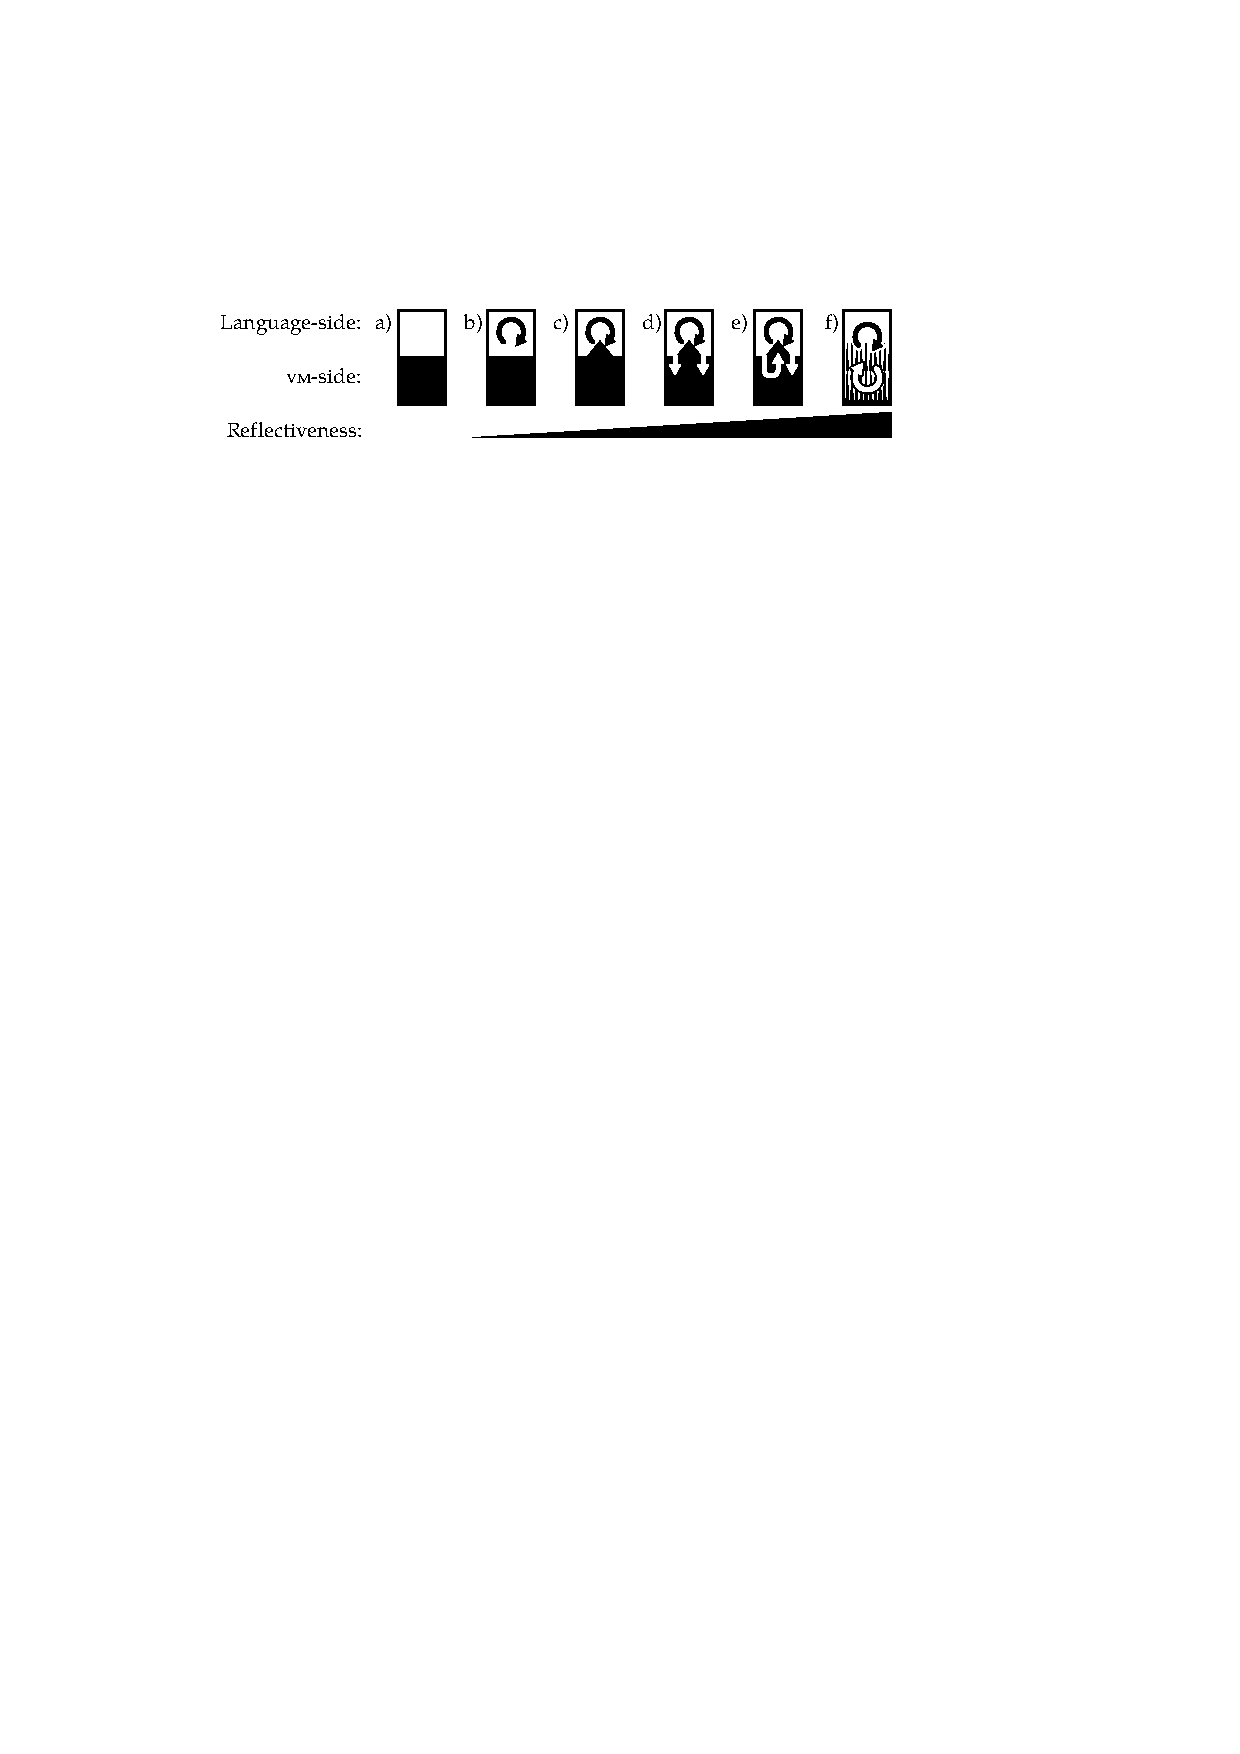
\includegraphics[scale=1.1]{vm-reflection-evolution}
	\figlabel{vm-reflection-evolution}
	\caption[High-level Language Reflection Evolution]{Evolution of reflection in high-level language runtimes.}
\end{figure}
%
\cb{recheck that the properties fit to what I told everybody}
\begin{enumerate}[a)]
\item \textbf{Language-side without reflection:} A language in this category requires a virtual machine to run but has no reflective properties.
	This includes early-stage languages such as the original Pascal-P system.
	Typically languages without reflection also lack the underlying \VM and are compiled directly to native code.
	\cb{thus they are one meta-level short of performing reflection}
	\sm{What's a VM? When does a runtime system become a VM?}
	
\item \textbf{Language-side with limited reflection:}
	The next step is to support only certain static reflection.
	This might include structural reflection whose required information can be prepared upfront during the compilation phase.
	\sm{What do you do with C++ and RTTI and direct access to memory? Isn't that what you want? Or is C++ OO programming not high-level enough? (You criteria are unclear)}
	Such a system has no support for unanticipated reflection as there is no support from the \VM to dynamically reify concepts.
	A \VM with a \JIT in this category can perform strong optimizations and take full advantage of the runtime information.
	\cb{GO fits here? \Java only partially?}
	
\item \textbf{Language-side extended reflection:}
	The third category of high-level language runtimes has extended reflection with strong support from the underlying \VM.
	We put \PH, \ST implementations or \Self in this category of languages.
	The \VM supports complex reification of otherwise non-accessible concepts \ugh{such as the stack}.
	\sm{The stack? What else, what distinguishes those systems? I have the feeling you want to define those distinctions for some purpose later on, which I don't know yet.}
	At this stage the \VM-level optimizations are a balance between restricting the supported language or sacrificing speed.
	
\item \textbf{Language-side access to the \VM:}
	The \VM support for reflection is highly extended compared to the previous category.
	Instead of a hidden property, certain \VM-level concepts are made explicitly accessible to the running language.
	Up to some extent this is similar to language-side structural reflection as the \VM only supports only a restricted interface which is defined at compile-time.
	\sm{What does that mean? Reading out performance counters? Doing VM level tracing, debugging? I can imagine plenty of examples that fit into this category}
	In this category the language can only read (introspect) \VM properties.
	\todo{MIST has a GC mop that fits in this category}
	To our best knowledge there are no existing language-runtimes that fall into this category.

\item \textbf{Language-side modification of the \VM:}
	The previous category allows the language-side to safely read \VM-level properties.
	If we follow the same path as the language-side evolution of reflection the next step is to allow for self-modification.
	Such a language-runtime has a dynamic interface to change certain properties of the \VM.
	However, the \VM is still not fully reflective in the sense that not all \VM concepts are reified.
	This essentially limits the language-side to simple interactions and changes to the \VM itself.
	At this point the \VM can no longer guarantee safety by isolating the language-side from all the low-level details.
	Again no systems are known to fit in this category.
	\sm{Still to vague for my taste, and I still can imagine things I would put into this category}
	
\item \textbf{Self-aware \VM:}
	We classify in the last category dynamic language-runtimes that have no longer a clear separation of \VM and language-side.
	The same reflective properties equally apply to language-side and the \VM.
	The way to achieve this is by flattening out the intermediate \VM and let the language-side directly control everything.
	Currently there are several research \VMs which can be classified as self-aware \VMs: The \P \VM \cite{Verw12a} is partially self-aware but in control of the underlying execution and the \Klein \VM is fully reflective \cite{Unga05a}. 
	\sm{What's with meta circular VMs, how do they fit in here? Some, I would say by accident, have properties that could be considered 'self-aware'.
	
	Further, I don't think those categories are disjunct. So, something that is self-aware is probably also in the previous categories}
\end{enumerate}

\noindent From this overview of reflective evolution of high-level languages we see that there is only little research about self-aware \VMs or reflective \VMs.
In general high-level languages are built with a clear distinction of the language-side and the \VM.
\sm{Where does the VMIL2011 paper fit in? Stephen Kell, I believe?}
However, with further reflective capabilities of the language-side we see that such a separation is no longer a guarantee for security.
In fact many security aspects have to be addressed already at language-side \cite{??}.
\sm{Why do you talk about security at all? Are you doing anything about it? If not, remove those discussions, and put them in future work, and the beginning somewhere needs to state that it is out of scope.}
This we want to focus in this thesis on the reflective aspects of the \VM.
In order to further compare reflection in languages we will now discuss the different \VM building approaches. 


% ===========================================================================
\section{Open \VMs}
\seclabel{background-open-vms}
% ===========================================================================

High-level language \VMs are inherent complex pieces of software.
They have to combine two rather extreme goals: abstraction and performance.
We have seen that the required abstraction for the running high-level language has a strong influence on the \VM design.
At the same time the hard performance requirement requires precise interaction with the underlying hardware.
This goes even so far that specialized hardware is conceived to match the performance requirements \cite{Clic05a}.
\sm{I don't like the way you cite. Ok, the cliff paper, good. Not a really good example thought, what about lisp machines, smalltalk, or java processors, or David Ungar's work in determining the benefit of processor support for high level languages?}

The early \VMs focused on interpreting an abstract instruction set (bytecodes).
The benefits are twofold.
On the one hand the bytecodes guarantee certain platform independence by abstracting away from the \CPU specific instruction set.
On the other hand bytecodes allow to encode complex operations into little space both serving the hard memory constraints of the hardware and simplifying the design of a compiler.
Obviously this abstraction gain comes at a cost and ever since the first \VMs were built research and industry strive to reduce the interpretation overhead.
An efficient way to improve performance is to use a just in time compiler (\JIT) that dynamically generates native code from the bytecode \cite{??}.
In this case the bytecode becomes an intermediate representation (\IR) for a bigger compiler infrastructure.
However, \JIT compilers are notoriously complex as they crosscut many \VM components.
At the same time they crosscut all abstraction layers; they have to access high-level information from the running bytecodes and manage native code at the same time.
Similar, albeit less low-level oriented complexity applies to the automatic memory management present in most high-level language \VMs.
Garbage Collectors (\GC) evolved from simple helpers to complex software artifacts that for instance support concurrent garbage collection \cite{Clic05a}.
\sm{Say what? GC less low-level complexity? Really? Pffff}

The increased complexity of the \VMs lead to more novel approaches on how to build \VMs.
\VMs are still build for a big part in C or C++ for performance reasons.
However, there are more high-level approaches that try to simplify creating \VMs by using building blocks \cite{Geof10a}.
\sm{Really? What is 26, I really need to jump through the PDF here? Not nice to your reader, not nice at all. If you got a point to make, make it explicit, not indirect. It is your text, you want to convey a message, do it precise and clearly, don't make me guess. If the point is not important, don't raise it.}
In the following sections we are shedding light on metacircular \VMs which are programmed in the same language they in the end support.

% ---------------------------------------------------------------------------
\subsection{Metacircular \VMs}
\seclabel{background-metacircular-vms}
% ---------------------------------------------------------------------------
\sm{Ok, a little late? I would have liked to know upfront that you are getting here as well.}
The ever growing complexity of \VMs and the abstraction mismatch between the \VM definition language and the final interpreted language lead to a new movement that tried to reduce complexity.
Among the \VMs using higher-level languages or frameworks to reduce the development effort the metacircular building process stands out.
Unlike the classical \VM which is built in C and compiled to the a binary, a metacircular \VM is written in the same language that it provides in the end.
The following figure highlights the most evident differences between a classical and a metacircular approach.
%
\begin{figure}[h]
	\centering
	\vspace{1mm}
	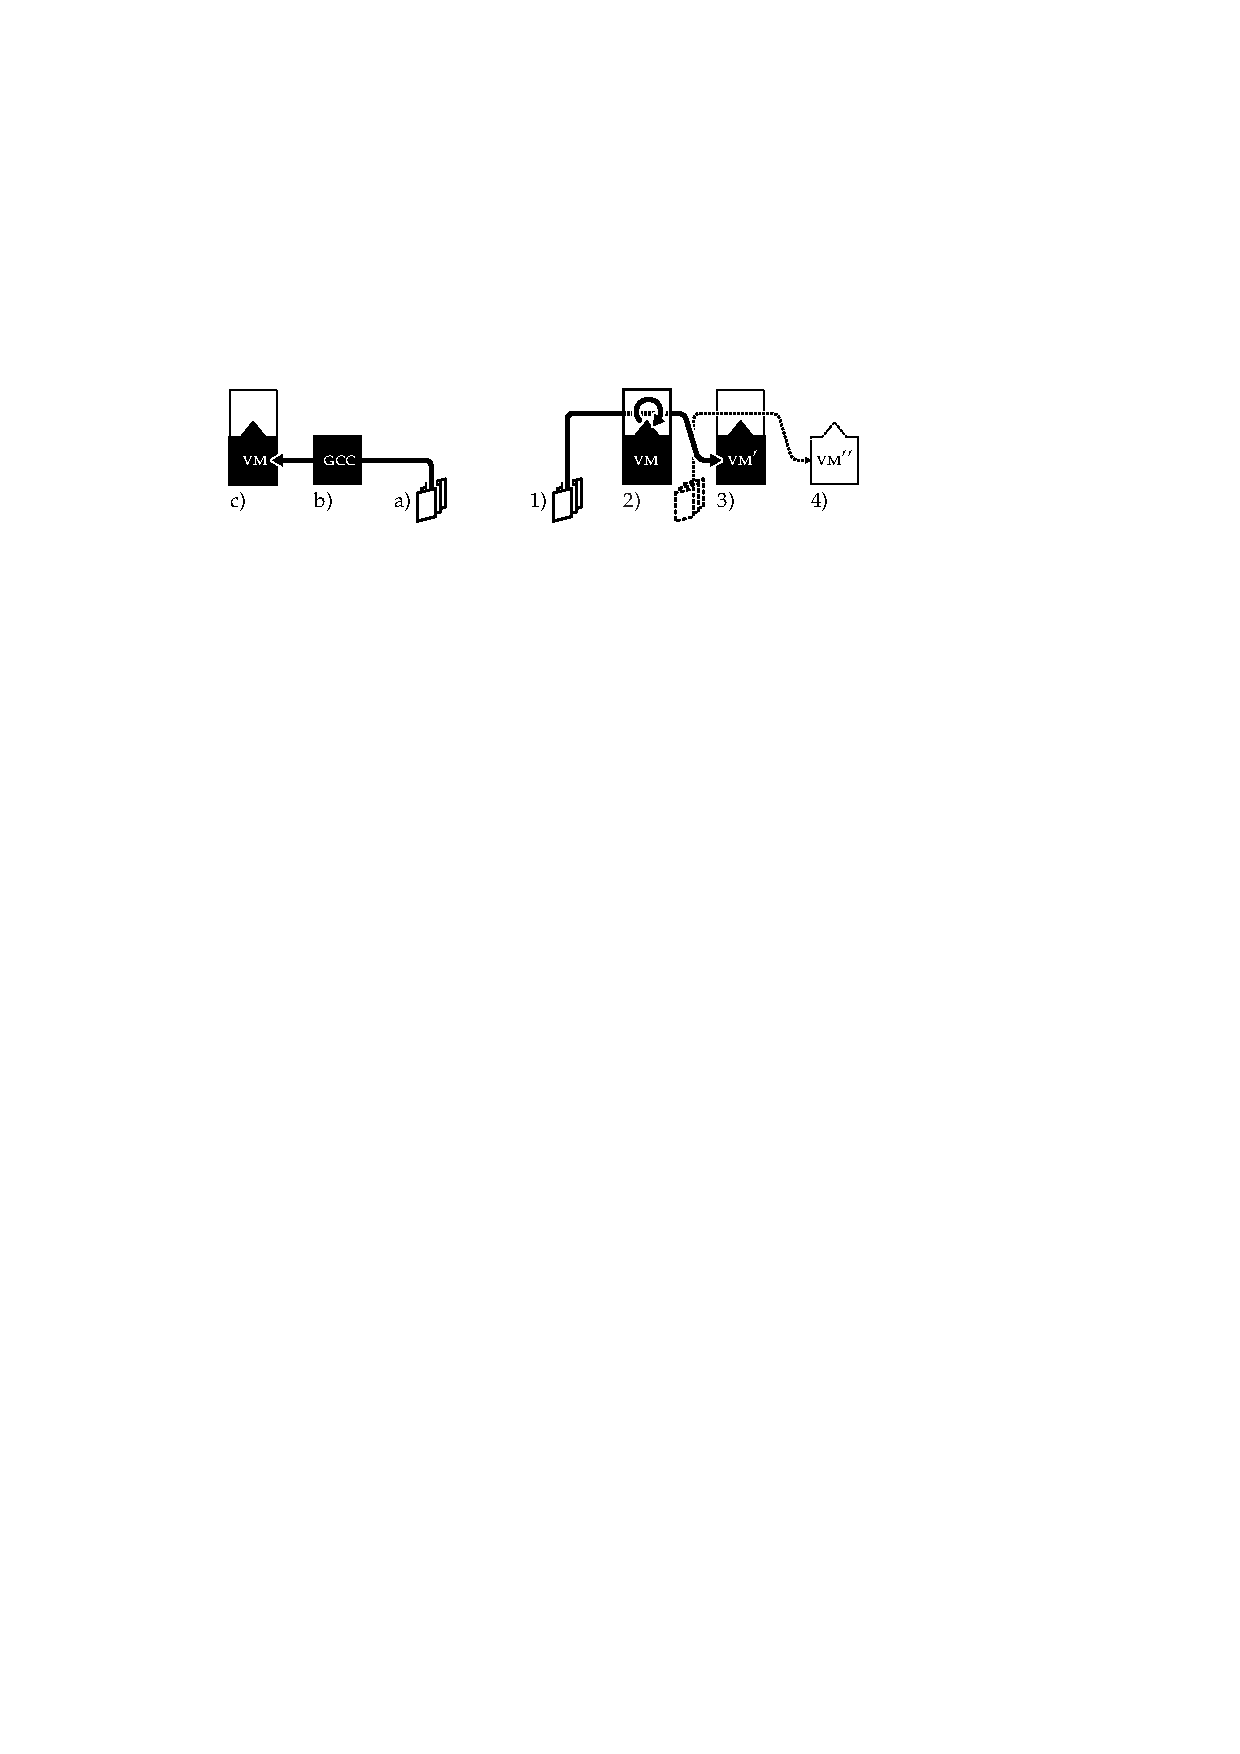
\includegraphics[scale=1.1]{vm-metacircular-building-process}
	\vspace{-5mm}
	\sm{Right to left? Strange order}
%	\figlabel{vm-metacircular-building-process}
\end{figure}
%
\begin{description}
\item[Classical \VM Compilation] \hfill
	\sm{Why is the compilation process the thing you focus on? Isn't that incidental? }
	\begin{enumerate}[a), nolistsep]
		\item \VM sources typically written in C or C++
		\item Compilation of the \VM sources using a C or C++ compiler
		\item Final Binary
	\end{enumerate}

\item[Metacircular \VM Compilation] \hfill
	\begin{enumerate}[nolistsep]
		\item \VM sources written in a high-level language, the same as the final \VM supports
		\item Compilation of the \VM sources happens by evaluating the \VM sources, allowing for compile-time reflection
		\item New \VM' binary built using an existing version of the \VM
		\item The new \VM Binary can be used to compile again a new \VM''
	\end{enumerate}
\end{description}

\noindent Using the same language for developing the \VM has several advantages.
Usually the \VM is in great contrast to language-side libraries on the same platform.
This is due to the low-level nature of the \VM.
Using a high-level language certain implementation details can be hidden.
Furthermore the metacircular approach provides the \VM developer with the same tools as a language-side programmer.
Typically this leads to faster development.


Inside the metacircular \VM community we see different approaches with varying levels of abstractions and reuse.
When compared, we find differences in how metacircular \VMs build \VM components (\GC, \JIT) and how the bootstrap or compilation of the new \VM works.
We see metacircular \VMs that use the high-level language as an advanced macro systems.
In a sense an extended version of C++'s templates.
Other approaches use the full reflective power of the high-level runtime to simplify code.
And even more advanced system automatically provide the \VM developer with \GC or a \JIT compiler.
We will now elaborate in more detail how metacircular \VMs are constructed.


\paragraph{Language Property Synthesis}
In the classical C-based \VM approach all \VM components have to be explicitly build.
Each \VM is a one of a kind with custom interpreter and a specialized memory manager.
Using high-level \VM frameworks it is possible to provide the \VM developer with prefabricated components.
For instance it is possible to simply parametrize a premade \GC to reduce development effort.
Looking at the evolution of metacircular \VMs we see both approaches.
For instance early metacircular solutions like the \Squeak \VM \cite{Inga97a} work more like a high-level C macro system.
\sm{I would not categorize squeak as metacircular, neither PyPy, which I missed so far in your discussion}
The high-level language is used to generate C code which is then further compiled to the final \VM binary.
\VM components are declared in a very explicit style, again not much different from C++.
Memory for \VM-level structures has to be managed in the same way as its C++ counterpart by explicitly allocating and freeing objects.
On the other side we have \VM frameworks like \PyPy for the \Python language that provide automatic \GC and \JIT support.
Here the developer writes a new \VM in almost the same way as a normal \Python program.
In the ideal case only certain hints are necessary to create a \JIT.

\todo{Truffle as extreme to that track: Interpreter implementation on \AST basis, not explicit bytecode interpreter (which would be typical in C)}

\paragraph{Bootstrap Process}
\sm{And bye the way, I forgot where you are going with all this. Why do I care about the bootstrap process?}
A crucial step during the development with the metacircular \VMs is the bootstrap of the new \VM.
We distinguish mainly between two approaches, indirect bootstrap and direct bootstrap.
%
\begin{figure}[h]
	\centering
	\vspace{2mm}
	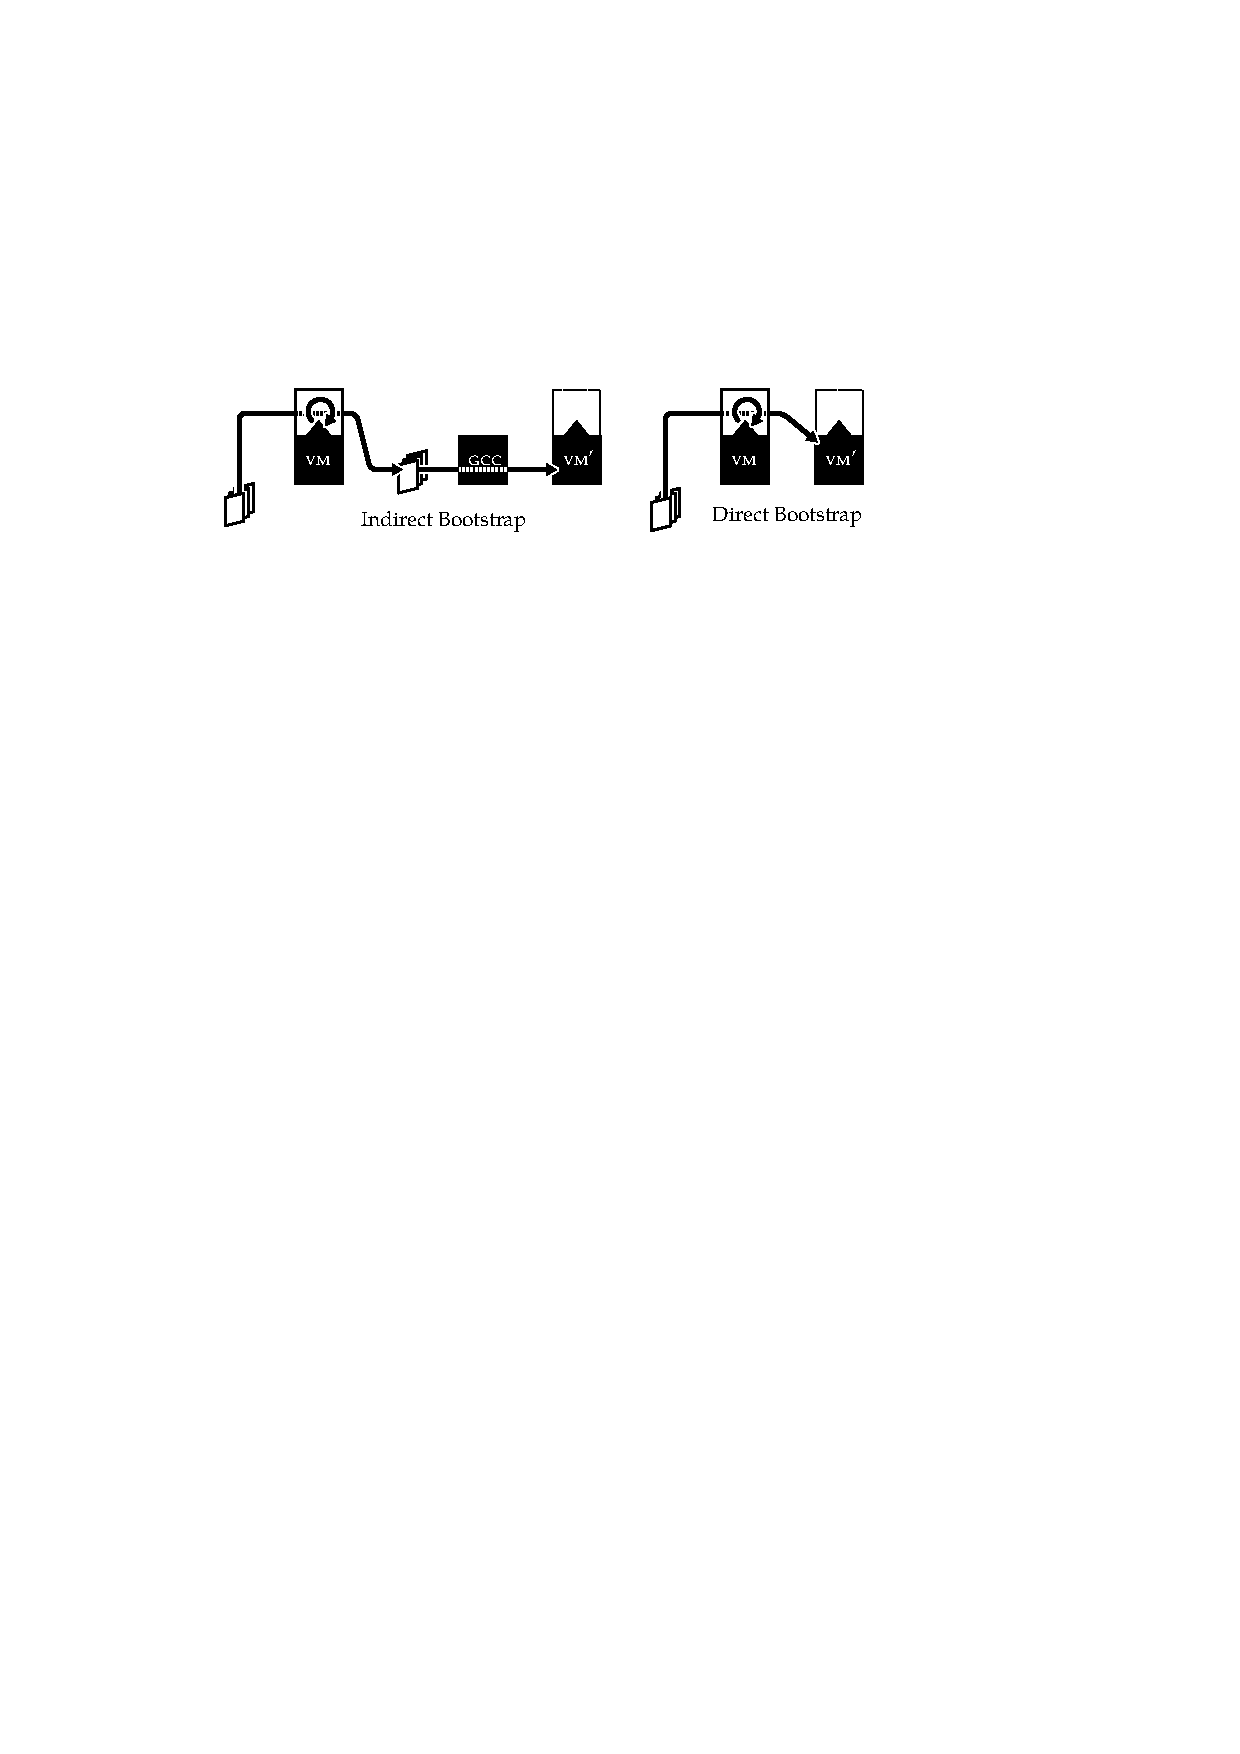
\includegraphics[scale=1.1]{vm-metacircular-bootstrap}
	\caption{Metacircular \VM Bootstrap Types}
	\vspace{-5mm}
	\figlabel{background-metacircular-bootstrap}
\end{figure}
%
\begin{description}
	\item[Indirect Bootstrap:] Metacircular \VMs with an indirect bootstrap use an intermediate language to compile a new \VM binary.
	A typical example of this approach is \Squeak and \PyPy using C.
	Both of these system imply a complete C compilation stack.
	The advantage of this approach is the that C is heavily optimized thus reducing the development effort for the \VM framework.
	However, C already hides a lot of low-level details away.
	Typically the \VM framework has to work around these limitations when working directly with native code for instance in the \JIT.
	We have explicitly seen these limitations while working on the \P \VM.
	
	\item[Direct Bootstrap:] Metacircular \VMs with a direct bootstrap are directly in charge of generating the native code for the final binary.
	We have seen in \P that many C-level optimizations have only limited impact on the final speed.
	A major speedup is achieved by using a native stack and directly generating native code instead of using a bytecode interpreter.
	Hence the \VM will probably require an assembler framework which in return can be used for the direct bootstrap.
	This means that only limited additional efforts are necessary for a direct bootstrap.
	As a result the direct bootstrap allows full control of how the final binary will look like.
	\sm{Neither using the stack directly, nor generating native code is specific to direct bootstrapping, it is entirely orthogonal. Your discussion and examples here are not consistent with the goal I perceive for this section }
\end{description}

% ---------------------------------------------------------------------------
\subsection{Compile-time Reified \VMs}
% ---------------------------------------------------------------------------
\sm{My questions at a beginning of a section are: why do I read it? What am I going to learn? And how does it fit with/supports the thesis goal?}
After presented the technical background of metacircular \VMs we are presenting several concrete implementations in more detail.
In this first part present \VMs that focus on compile-time reflection.
In \secref{background-reified-vms} we will then focus on a list of \VMs that reify their components and allow for a more close interaction with the language-side.


\subsubsection*{\Squeak \ST \VM}
\seclabel{background-squeak}
% ---------------------------------------------------------------------------
\sm{I still don't take squeak as metacircular in the strict sense. For me, that means  implemented in itself. Java with java, lisp with lisp, smalltalk with small talk, squeak is implemented in slang, that's C with smalltalk syntax, which is barely executable as smalltalk, PyPy is implemented with RPython, also restricted subset, and with its type system, I would say, a very different language. You can however make the point that RPython is a strict subset of Python, and thus, without changes directly executable. That's not true for Slang...}
One of the first metacircular \VMs presented is the \Squeak \VM\cite{Inga97a}.
Its core building system is still in active use for the \urlfootnote{\Cog \VM}{http://www.mirandabanda.org/cogblog/} which extends \Squeak with a \JIT.
The \Cog \VM is used as default by the \urlfootnote{\PH}{http://pharo.org/} programming language.
\Squeak is built around a \ST dialect called \Slang that is exported to C to be compiled to the final \VM binary.
Additionally the \Slang sources can be interpreted to provide an interactive simulator of the \VM, including full graphical support.

The \VM itself is mostly written in a dialect of \ST \sm{You just said that} called \Slang that is essentially limited to the functionality that can be expressed with standard C code.
\Slang in this case is mostly a high-level C preprocessor.
Even though \Slang basically has the same syntax as \ST it is semantically constrained to expressions that can be resolved statically at compilation or code generation time and are compatible with C.
Hence \Slang's semantics are closer to C than to \ST.
Unlike later metacircular frameworks \Squeak uses little or no compile-time reflection to simplify the \VM designs.
However, class composition and traits help structuring the sources.
\sm{Traits aren't used, are they?}
Next to the \Slang source which account for the biggest part of the interpreter code some \OS-related code and plugins are written in C.
To facilitate the interaction with the pure C part \Slang supports inline C expressions and type annotations.
\sm{Why is all of this important here? Does not seem to contribute to your discussion }

A great achievement of the \Squeak \VM is a simulator environment that enables programmers to interact dynamically with the running \VM sources.
The simulator is capable or running a complete \Squeak \ST image including graphical user interface.
This means that programmers can change the sources of the running \VM and see the immediate effects in the simulator.
The simulator itself works by setting up a byte array which servers as native memory.
Then the \VM sources written in \Slang are interpreted by the \VM of the development environment.

We see that \Squeak is an early-stage metacircular \VM that uses an indirect bootstrap process.
Yet according to long-time \VM programmers the \Squeak infrastructure is more productive than a comparable C++ or pure C project.
\sm{Early stage? Common, true metacircular implementations are much older, squeak is a step back in terms of pure ness of concepts}


% ---------------------------------------------------------------------------
\subsubsection*{\Jikes: High-level low-level Programming in with \MMTK}
\seclabel{background-jikes}
% ---------------------------------------------------------------------------
\Jikes (former \textsc{Jalapeño})is an early metacircular research \VM for \Java \cite{Alpe00a}.
The \Jikes \VM features several different garbage collectors and does not execute bytecodes but directly compiles to native code.
\sm{Why is that relevant? Think, you are implying something here?}

The \Jikes \VM had performance as a major goal, hence direct unobstructed interaction with the low-level world is necessary using a specialized framework.
High-level low-level programming \cite{Fram09a} is mentioned the first time in the context of the \Jikes \VM project.
The goal of high-level low-level programming \ugh{is to the} abstractions provided by high-level programming languages to simplify low-level programming specifically.
\ugh{In the core this are} the same motivations that drives the metacircular \VM community.

Frampton et al. present a low-level framework packaged as \ttt{org.vmmagic}, which is used as system interface for Jikes, an experimental \Java \VM.
Additionally their framework is successfully used in a separate project, the memory management toolkit (\MMTK) \cite{Blac04a} which is used independently in several other projects.
The \ttt{org.vmmagic} package introduces highly controlled low-level interaction in a statically type context.
In their framework, methods have to be annotated to enable the use of low-level functionality.

In a direct metacircular \VM building process (see \figref{background-metacircular-bootstrap}) it is inevitable to directly manage native-code.
Using a high-level low-level framework provides the necessary abstraction at this level.
\sm{Shouldn't that go with the motivation paragraph? One paragraph up?}

% ---------------------------------------------------------------------------
\subsubsection*{\Maxine \Java \VM}
\seclabel{background-maxine}
% ---------------------------------------------------------------------------
\Maxine is a metacircular \Java \VM \cite{Wimm13a} focused on an efficient developer experience.
Typically \VM frameworks focus on abstraction at the code-level which should yield simpler code and thus help reducing development efforts.
However, in most situations the programmer is still forced to use existing unspecific tools for instance to debug the \VM.
In contrast to that, the \Maxine \VM provides \ugh{first-hand tools} to interact with the \VM in development.
\Maxine uses abstract and high-level representations of \VM-level concepts and consistently exposes them throughout the development process.
Inspectors at multiple abstraction levels are readily available while debugging, giving insights to the complete \VM state.
\Maxine provides and excellent navigation for generated native code by providing links back to language-side objects as well as other native code and symbols.

Even though the \Maxine projects follows an approach where reflection is only used at compile-time, the development tools themselves provide a live interaction with the running \VM artifact.
\sm{And this distinction is important, reflection != the ability to observe and interact with (cf. JVM tooling }
This means that when debugging the \VM it behaves almost like a life \ST image where a complete interaction with the underlying system is possible.
We identify this as crucial, as most of the time is spent debugging, notably on inadequate tools like \ttt{gdb} due to lack of alternatives.
\sm{Connect this to your problem statement (back reference) and, make sure your problem statement does not mix up reflection and observability/interactivity }
Hence having a specific debuggers and inspectors greatly improve the interaction with the \VM artifact.

\subsubsection*{\PyPy Toolchain}
\seclabel{background-pypy}
% ---------------------------------------------------------------------------
\urlfootnote{\PyPy}{http://pypy.org/} is a \Python-based high-level \VM framework \cite{Rigo06a}.
\PyPy's major focus lies on an efficient metacircular \Python interpreter.
However, it has been successfully used to build \VMs for other languages including \ST \cite{Bolz08a}.
Interpreters are written in a type-inferable subset of \Python called \RPython.
The underlying \PyPy infrastructure implicitly provides memory management and \JIT compilation.

\paragraph{Provided \VM Features}
\PyPy follows a different approach from the previously presented \VM generation frameworks.
For instance, in Squeak and \Jikes the final \VM implementation is not much different from C or C++.
\sm{C/c++ has nothing to do with this

It is about direct implementation vs. composition by a tool chain or something similar. At least that's my understanding here}
The programmer specifies all the components of the \VM explicitly, either by implementing them directly or using a provided library.
Compared to the more static C ans C++ these \VM generation frameworks make the compilation phase more tangible.
\ST in \Squeak or \Java in \Jikes or \Maxine fulfill the purpose of the template system in C++ or the restricted macro system in C.
For the explicit implementation part \PyPy is no different.
However, certain features for the final \VM are directly absorbed from the underlying \PyPy infrastructure.
For instance, the \JIT support or the \GC are not explicitly implemented but provided by the \PyPy framework itself.
This is a big difference to the other \VM frameworks as it allows programmers to write the \VM in a more high-level fashion.
For instance in \Squeak memory allocation, even for \VM-level objects, has to be handled in the same way as in C.
Whereas in \PyPy the garbage collection is left to the underlying infrastructure.
\sm{This paragraph needs to be revised, your line of argumentation is confusing/conflating many different aspects, and that does leave a bitter taste to me as a reader}


\paragraph{\RPython Interpretation}
At compile-time the interpretation stack for a newly implemented \VM on top of \PyPy looks as follows.
\sm{Why do I care for those details?}
%
\begin{enumerate}
\item The final language runtime
\item The \VM written in \RPython
\item The \PyPy infrastructure (virtual compile-time \RPython interpreter)
\sm{These terms don't mean anything to me? Which part is which? What's the implemented language? Concrete example?}
\end{enumerate}
%
Unless in debug mode, the bottom-most layer is compiled away by exporting the \RPython sources to C.
However, before the C export step, all the compile-time reflection statements are evaluated and flattened away.
This approach allows \RPython \VMs to behave almost like standard \Python programs while still providing excellent performance in the final \VM binary.

\paragraph{High-level Tracing \JIT}
Much like the automatic memory management, \PyPy provides a tracing \JIT generator \cite{Bolz09a}.
By default the \VM programmer does not write an explicit \JIT in \PyPy.
Instead the \VM code is annotated to guide the underlying tracing \JIT generator.
This means a \VM compilation time a specific tracing \JIT is created for the given meta information.
As a result, the \JIT can track high-level loops in the final interpreted language.
\sm{What's the similarity between GC and tracing JIT? One traces object graphs the other traces operations, two totally different things

Aaaaah, it is provided as a service, implicitly, ...
Ok, make that explicit, say something like that}


% ---------------------------------------------------------------------------
\subsection{Runtime Reified or Self-aware \VMs}
\seclabel{background-reified-vms}
% ---------------------------------------------------------------------------

The \VMs presented so far have little or no self-awareness.
\VM generation frameworks allow a high amount of reflection at \VM compile time.
This meta information is typically compiled away.
This is somewhat similar to what happens with templates in a C++-based \VM.
The \VM frameworks themselves behave like a static language on their own.
As a result, the final \VM artifact has no access to the underlying definition anymore.

As an example we might have several \VM components represented as high-level objects at compile or \VM generation time.
These objects have a class and methods attached, information that is reflectively accessible.
However, once the \VM is compiled down to native code, most of this information is lost.
What is left is native code with low-level instructions that allow little or no reasoning about the original high-level structure.
\sm{This is way to general and unspecific, and  I am not sure why that's discussed here}

We have shown in \secref{background-vm-reflection} how a potential evolution of reflection in a high-level language looks.
We concluded that the evolution of language-side reflection implies a similar evolution at \VM-level.
More behavioral reflection at language-side requires more concepts to be reified in the \VM itself.
This requirement is conflicting with the previously described loss of reification at \VM-level.

We are now going to present \VMs that behave significantly different.
Unlike the previous ones, they no longer make a clear distinction between the static \VM and the dynamic language-side.


% ------------------------------------------------------------------------------
\subsubsection*{\DwarfPython}

\DwarfPython \cite{Kell11a} is a \Python implementation that aims at a barrier-free low-level interaction.
It emerged from an earlier \textsc{Parathon} which used \Dwarf debugging information from external libraries to facilitate foreign function interfaces.
\DwarfPython takes this idea further.
Additionally to describe low-level code, \DwarfPython uses the \Dwarf metamodel to describe \Python code and data.
This is depicted in \figref{background-dwarf-python}.
%
\begin{figure}[h]
	\centering
	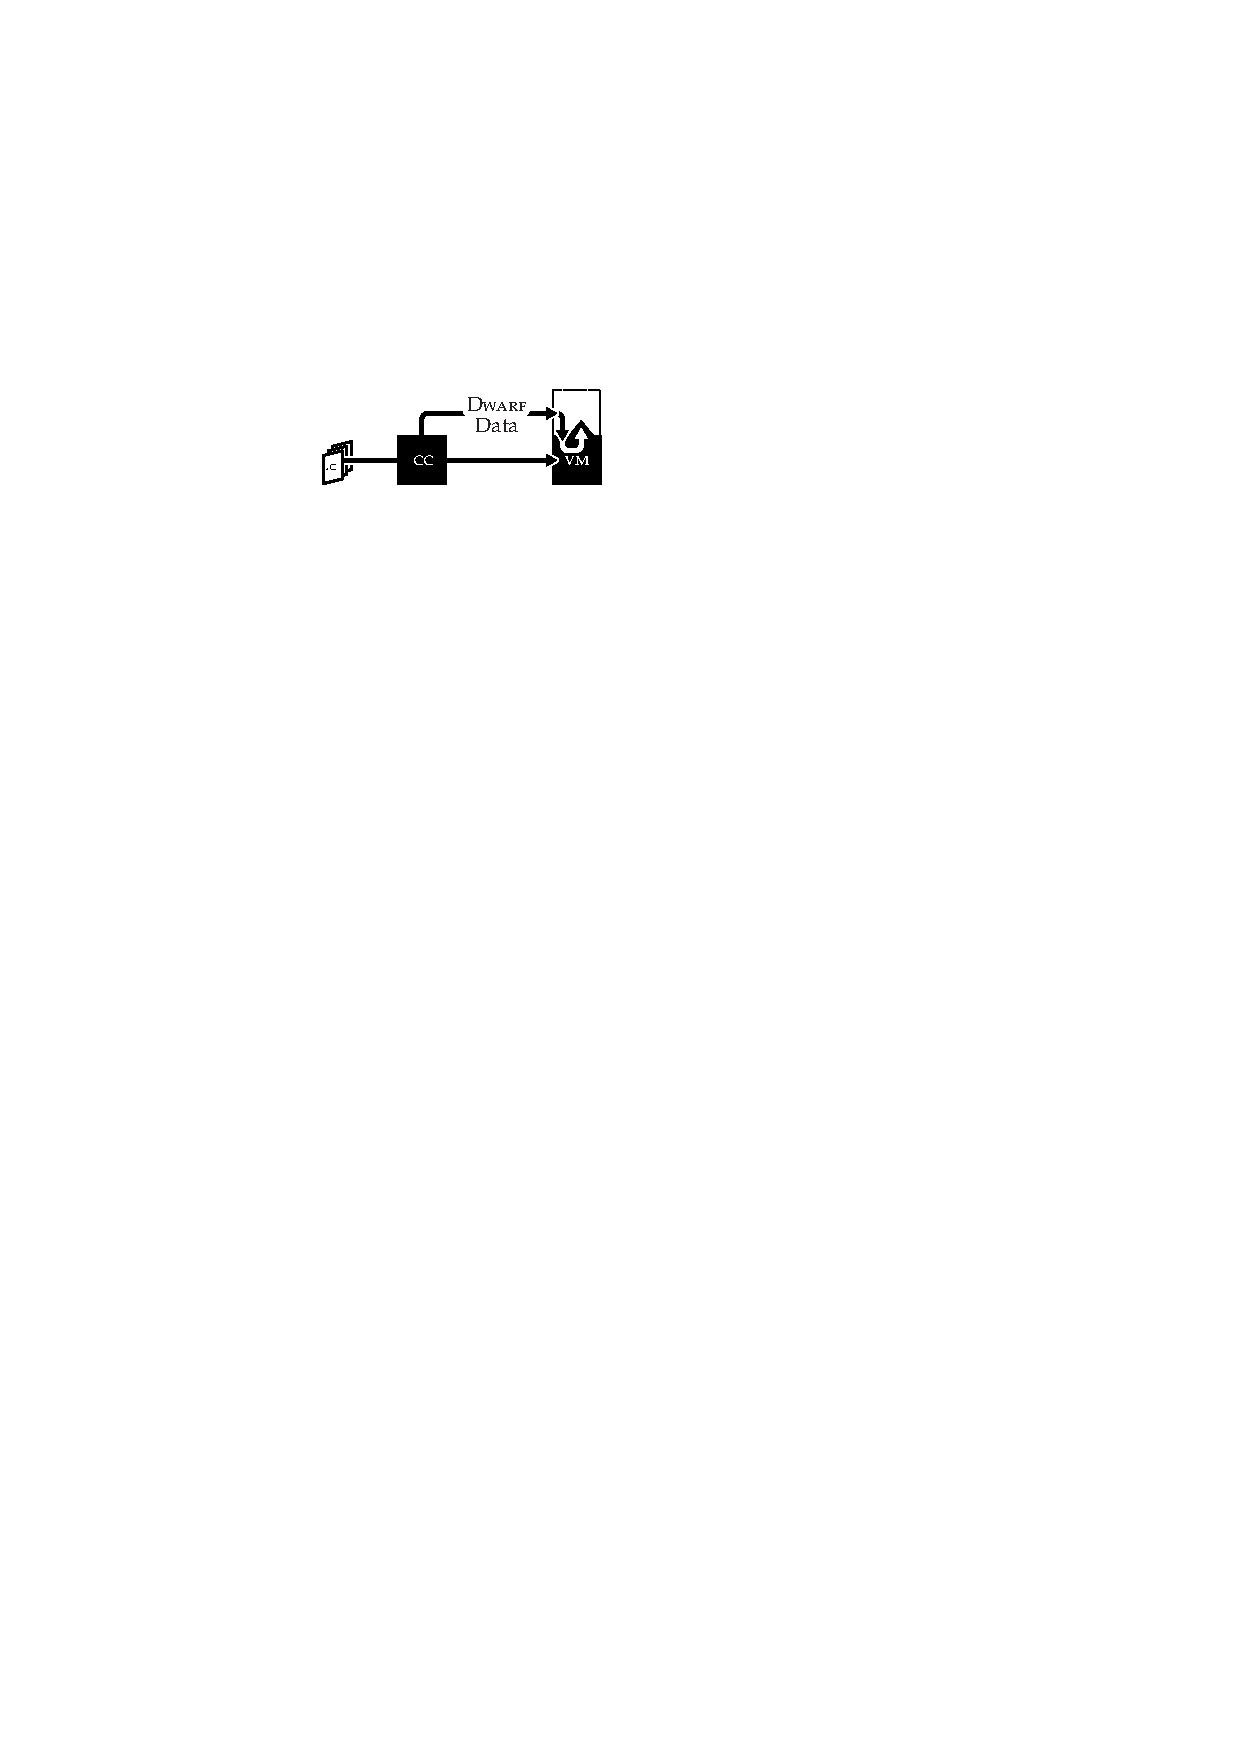
\includegraphics[scale=1.1]{vm-dwarf-python}
	\caption[\DwarfPython Low-level Reification]{\DwarfPython reifies the low-level \VM by using the \Dwarf Debugging information at language-side.}
	\figlabel{background-dwarf-python}
\end{figure}
%
This approach has the advantage that the very same debugging mechanism applies for low-level code, for instance written in C, and for high-level \Python code.
Thus \DwarfPython essentially unifies the previously decoupled \VM with the language-side.

% ------------------------------------------------------------------------------
\subsubsection*{\Pinocchio \VM}
\seclabel{background-pinocchio}

\P \cite{Verw11a} is a research \ST environment that directly uses native code instead of bytecodes.
The only execution base is native code which is directly generated by the language-side compiler.

\P is built from a kernel derived originally from a \PH image.
For the bootstrap classes, objects and methods are exported into binary, native images and linked together with a standard C linker to a final executable.
For simplicity we also rely on a very small part of C code to provide essential primitive, for instance used for file handling.
Additionally we specified part of the bootstrap for the \ST object model in plain C code.
However, besides that, all the other code is written and developed directly in \ST.
%
\begin{figure}[h]
	\centering
	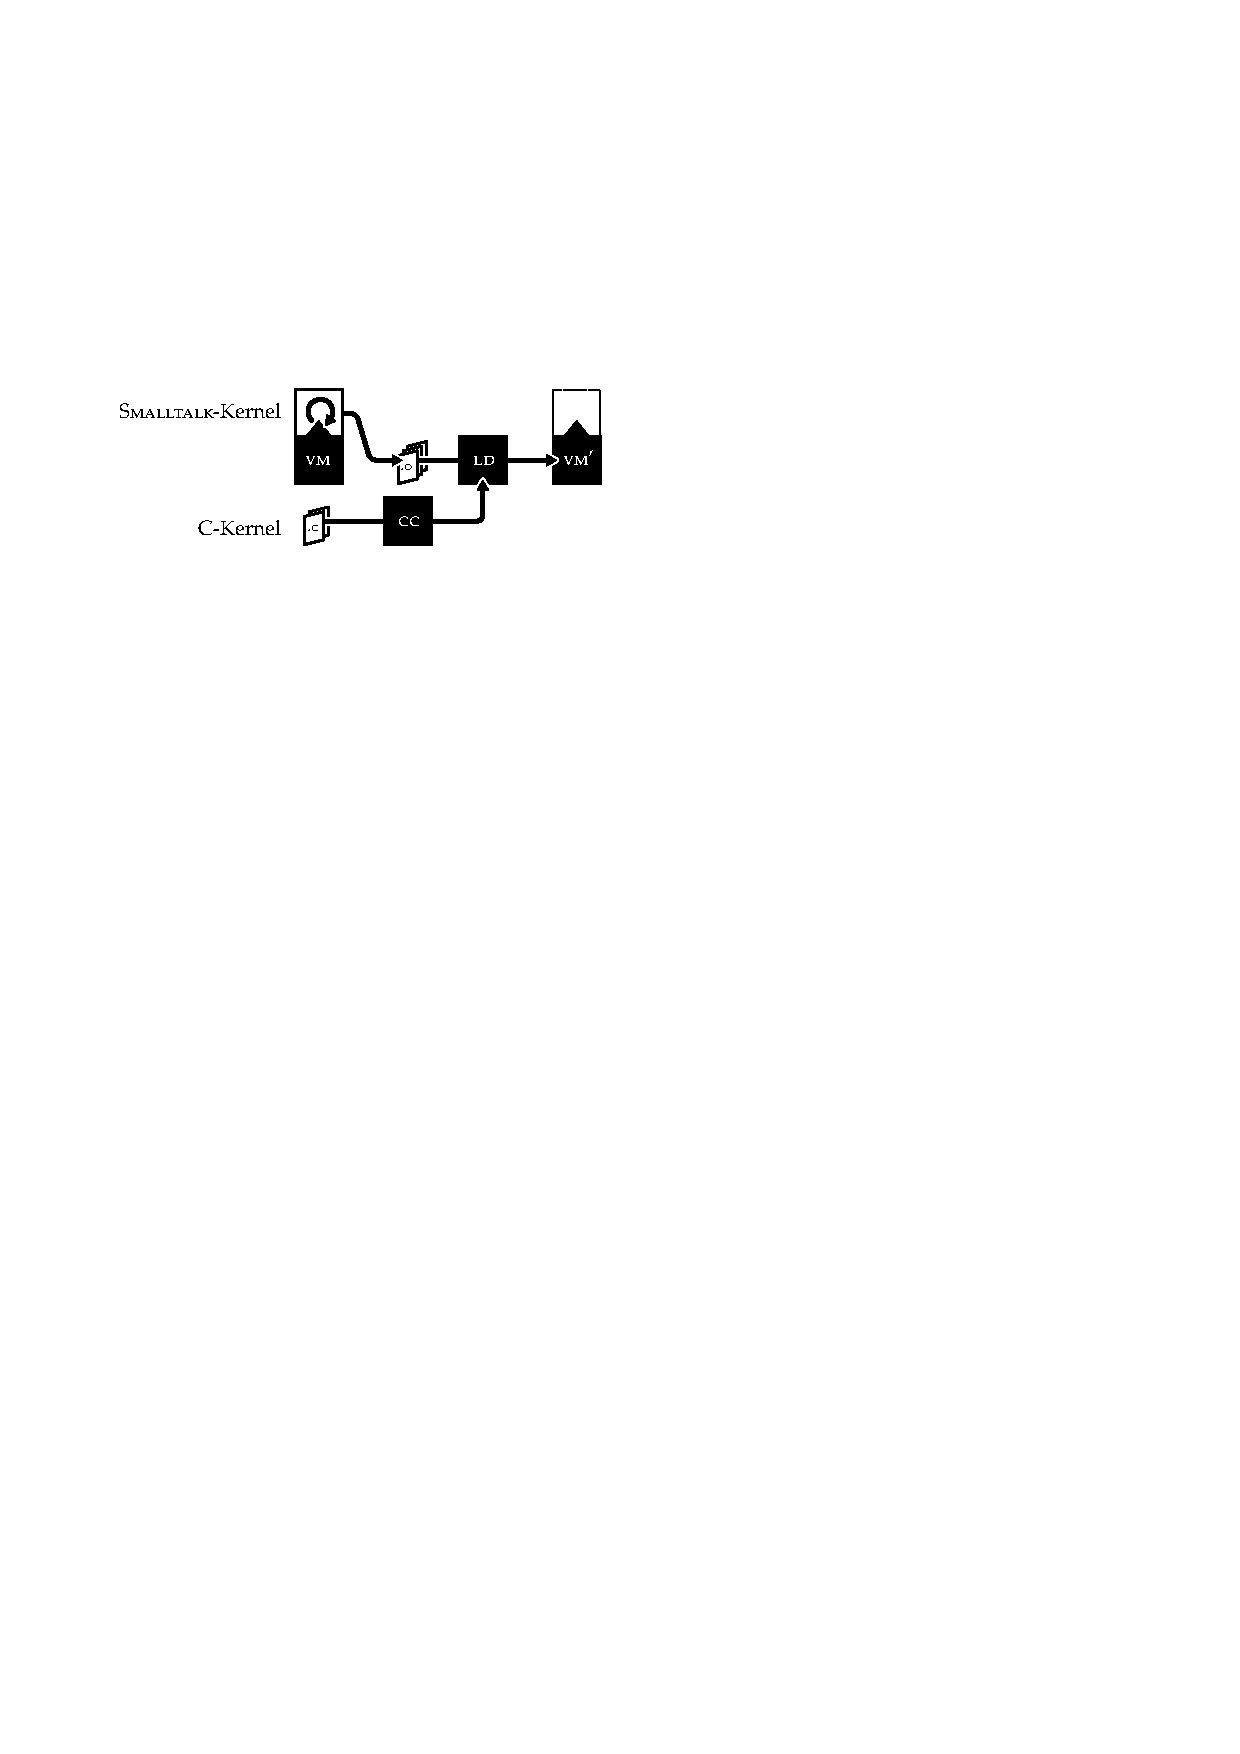
\includegraphics[scale=1.1]{vm-pinocchio-bootstrap}
	\caption{\P's Bootstrap}
	\figlabel{background-pinocchio-bootstrap}
\end{figure}

An important aspect of \P is that the method lookup is expressed in terms of normal \ST code.
Typically this code statically resides in the \VM, thus at a different meta-level.
Hence this implies for most systems that the lookup can not be modified without altering the \VM itself.
However, expressing the lookup in terms for normal language-side code introduces a recursive dependencies during the bootstrap.
In order to run the lookup code expressed in \ST code, we have to perform message sends.
These, in return, require an already working lookup mechanism.
Hence, without a taking special care, a language-side lookup method will lead to infinite recursion during startup.
We resolved this problem in \P by directly interacting with the low-level execution format which among other things relies on inline caches to improve performance.
The important property of inline caches is that they bypass the slow language-side lookup by directly jumping to the last activated method at a send-site.
This is exactly the behavior we need to prevent recursion during the startup.
Hence, when generating the native code for the bootstrap, we prefill all the inline caches of the methods required to perform a full method lookup.
As a result, when running requiring the first real method lookup, the lookup code itself is running perfectly on the prefilled inline caches.
\sm{Ok, cool, how is that relevant in this context?}

From an architectural point of view, \P is performing almost a direct bootstrap.
Besides the small C kernel, the language-side code is directly compiled to native code.
As a result, \P only requires a single compiler for native code, during bootstrap and at runtime.
Hence, a separate \JIT implementation is not required.

The most obvious shortcoming of \P is the lack of its own garbage collector.
Instead of investing time into a separate well-defined \GC \P relies on the conservative \urlfootnote{Boehm \GC}{http://www.hpl.hp.com/personal/Hans_Boehm/gc/} built for C programs.
The Boehm \GC is sufficiently fast to run \P as a prototype, however, due to its generic nature it is not as efficient as a specific \GC.
However, \P lacks the necessary reification at level of the object layout to properly implement a \GC.
\sm{Why does that matter? And why is 'efficiency' relevant  here?}
All the notion about the object layout in memory are hard-coded in the compiler in several places.
Work was undertaken to put first-class object layouts in place and delegate memory allocation and field access to these meta objects.
Yet, at the current state \P has not incorporated this in the compiler core.
\sm{The whole section over and over again, you are first talking about something that's on its own only barely relevant, and then afterwards you make it relevant to me as a reader. Your writing could improve a lot by following classic paragraph structure: title sentence, main argument,mans then details and/or examples + supporting arguments.

To proof your thesis is your only goal, I would prefer if everything is explicit or at least implicitly written to make }

\P is self-aware in the sense that it controls  native code generation and lookup at a single abstraction level.
There is no distinction between \VM-level code and language-side code.
\sm{What does generation and modify ability of inline cache content have to do with self-awareness? his is still unclear to me, generation especially, reflecting on inline caches, I do understand. 

I have the feeling the conceptual model you outline in the beginning needs more elaboration and details.

And the criteria then could benefit this discussion to make it more precise (a few back references)}

% ------------------------------------------------------------------------------
\subsubsection*{\MIST a C-less \ST Implementation}
\urlfootnote{\MIST}{http://mist-project.org/} is another prototype \ST \VM that follows similar goals as the \P \VM.
As well, it no longer uses a bytecode interpreter but only relies on native code.
However, it goes one step further than \P by not relying on any C-based infrastructure.
\MIST implements its own linker to build the final executable.
Hence unlike \P it does not require kernel primitives written in C.
\MIST brings its own implementation to directly perform system calls from within the language.
\sm{Why is it relevant? It is barely a paragraph, feels like it doesn't fit in or is underrepresented here. Also, instead of being indirect about the goals, it would help to restate them}

% ------------------------------------------------------------------------------
\subsubsection*{\Klein \VM}
\seclabel{background-klein}

\urlfootnote{\Klein}{http://kleinvm.sourceforge.net/} is a metacircular \VM for the \Self programming language that has no separation into \VM and language \cite{Unga05a}.
\Klein performs a direct bootstrap (see \figref{background-metacircular-bootstrap}) much like the aforementioned \P or \MIST \VM.
Hence \Klein does not use an intermediate low-level language to bootstrap the system.
\sm{I still don't get the point about the low-level IR/byte code being one of the hints you pick on.

It is an exchange format, a serialization, what ever, I think you want to make the point that it is not being executed? Well, I am not to sure about that for Klein...}

It is important to point out that the \VM-level structures and objects are not compiled away as it is usually the case.
Instead the \VM structures are represented as real \Self objects.
Hence the \Klein \VM supports true \VM-level reflection since there is only a single code base.
\sm{I don't like the 'compiled away'. In hotspot, everything is a C++ object! no? I think, you'll probably have clarified that point in text that comes earlier, so, I would avoid such 'sloppy' language here and use the precise criterion/terminology from earlier}

Additionally to the advances in reflection and metacircularity, \Klein focuses on fast compilation turnarounds to allow for a responsive development process.
Which is unlike for instance the \Squeak \VM where a full \VM bootstrap takes an order of minutes on modern hardware.
\Klein also supports advanced mirror-based debugging tools to inspect and modify a remote \VM.

Development on the \Klein \VM seized in 2009 and left the \Klein \VM in fairly usable state.
Like \P it currently lacks a dedicated \GC.
Yet, it proved that it is possible and build a language-runtime without a proper separation of the language-side and the \VM or base-level.
\sm{Proper is the wrong word here, proper has a positive connotation, also implying it is necessary}
From the literature presented about the \Klein project we see a strong focus on the improvements of the development tools.
The fact that the language-runtime allows \VM-level reflection to change the \VM dynamically is not directly mentioned in the literature.
While we see the practical limitations of changing the \VM at runtime we would like to open the doors to this new form of reflection.


% ===========================================================================
%\newpage
\section{Problem 1: Dynamic High-level Low-level Programming}
% ===========================================================================
We have seen in the presented \VMs that a tight integration with the low-level code is indispensable.
Relying on an intermediate solution such as C with inlined assembler expressions does not scale well.
Typically it is troublesome to circumvent the aggressive optimizations applied by the C compiler in order to get the desired native code.

When working with metacircular \VMs it is natural to implement a framework for maintaining the low-level code.
Such high-level low-level programming \cite{Fram09a} is used at compile time or \VM generation time to create the necessary native code.
However, we have seen that the same frameworks are not directly available in the final language-runtime.
The \JIT might make use of such a framework at runtime, though that part is hidden in the \VM itself.
Hence we see an opportunity to use high-level low-level programming in a dynamic context and at language-side to implement new functionality.
\sm{Is that so, in the java examples, the framework is a java library, no? Who prevents you from using it?

This problem needs to be clarified, it is to vague.
It needs to be crisp enough to directly, and trivially derive a evaluation from }


% ===========================================================================
\section{Problem 2: Extending Reflection by High-level Low-Level Programming}
% ===========================================================================
In the case of the classical separation of the \VM from the language-side, reflection stays isolated at language-side.
However, this is different in a self-aware language-runtime supporting a reflective language.
Due to the lack of clear separation between language-side and \VM-side, the same or almost the same reflective properties should apply to both sides.
Though this is a rather idealistic goal, as we have identified only few research \VMs that have a unified model and thus are self-aware.
\sm{Strict? Be careful with your wording, clear also implies something positive.
I want a clear separation, but not a strict one!!!}

We have identified that for instance the \Klein \VM would be perfectly capable of performing reflection on components that typically belong to the \VM.
\sm{Again, what's your definition, what are your criteria.

Much to vague for my taste...}
However, to our best knowledge we could not identify any publicly available work that leverages this fact.
\sm{Indeeded to retread this a couple of times, only the very first sentence mentions the problem, and then, you say Klein solves it. Well,that's no good...

Also, make the problem and goal discussion distinguishable, otherwise, you got a hard time to derive your evaluation criteria from it.}


% ===========================================================================
\section{Problem 3: Dynamically Changing \VM Components}
% ===========================================================================
Following from the previous problem statement, we can use the reflective capabilities, namely intercession, to alter the \VM itself.

\todo{moar}\\
\todo{How far can we go with this?}\\
\todo{Not even the \Klein VM talks about changing / interacting with \VM components}\\
\todo{What are the possible components to attack?}\\
\todo{The \JIT already naturally lives a hybrid live between VM and language-side reflection (especially in Pharo)}


% ===========================================================================
\section{Summary and Outlook}
% ===========================================================================

In this chapter we gave an overview of the related work of this thesis.
We started by outlining the concepts of reflection and what implications it has on the performance.
We have shown have partial behavioral reflection is used to limit the costs of reification.
Out of this we have seen that for many reflective features specific \VM support is required.
Thus we presented in \secref{background-vm-reflection} a detailed description on how the evolution of reflection affects the \VM.
At the end of the scale we describe a language-runtime that has no longer a clear distinction between language-side code and an isolated \VM.
In such a self-aware \VM or unified language runtime, reflection equally affects the language-side and the \VM.

In the second part of this chapter we discussed existing \VM implementations.
We focus on metacircular \VMs as they are already a good match to a unified language runtime.
They use reflection at compilation time to simplify the process of building a \VM.
However, even though reflection is widely used in these frameworks, it is restricted to the compile time.
The final \VM artifact has no reflective capabilities, it only provides the necessary interface to enable reflection at language-side.
Hence, we present in a second group \VMs that focus on a unified model.


We addressed the identified problems in the following way:
\begin{description}	
%	\item[\chapref{reification}] focuses on language-side applications that simplify the interaction with the low-level code.
%	We present a custom inspector framework that is required to visualize low-level structures.
%	As a second part we explain how we introduced first-class layouts and slots to \PH to reify the low-level structural layout of objects.
%	Both projects are crucial for metacircular \VM development and are direct results from the research conducted on the \P \VM.
	
	\item[\chapref{benzo}] describes a dynamic high-level low-level programming framework named \B.
	The core functionality of \B is to dynamically execute native-code generated at language-side.
		
	\item[\chapref{ffi}] presents \NB, a stable foreign function interface (\FFI) implementation that is entirely written at language-side using \B.
	\NB is a real-world validation of \B as it combines both language-side flexibility with \VM-level performance.
	
	\item[\chapref{validation}] focuses on two further \B applications that extend the reflective capabilities of \PH using high-level low-level programming.
	In the first part we present \WF a framework for dynamically generating primitives at runtime.
	\WF extends the concept of metacircularity to the running language by reusing the same sources for dynamic primitives that were previously used to generate the static \VM artifact.
		
	In a second part of \chapref{validation} we present \NBJ a prototype \JIT compiler that is based on \B.
	\NBJ shows the boundaries of the \B, yet we are able to interact with a \VM internal component.
\end{description}


% =============================================================================
\ifx\wholebook\relax\else
    \end{document}
\fi
%\documentclass[a4paper,12pt,twoside]{../includes/ThesisStyle}
\usepackage[utf8]{inputenc}
\usepackage[T1]{fontenc}

\usepackage[left=1.5in,right=1.3in,top=1.1in,bottom=1.1in,includefoot,includehead,headheight=13.6pt]{geometry}\renewcommand{\baselinestretch}{1.05}


% =============================================================================
%\usepackage[sectionbib]{chapterbib}	% Cross-reference package (Natural BiB)
%\usepackage{bibunits}
%\usepackage{natbib}					% Put References at the end of each chapter
\usepackage{algorithm}
\usepackage{alltt}
\usepackage{amsfonts}
\usepackage{amsmath}
\usepackage{amssymb}
\usepackage{cite}
\usepackage{color}
\usepackage{enumerate}
\usepackage{booktabs} % used for \midrule
\usepackage{fancyhdr}					% Fancy Header and Footer
\usepackage{graphicx}
\usepackage{ifthen}
\usepackage{latexsym}
\usepackage{multirow}
\usepackage{rotating}					% Sideways of figures & tables
\usepackage{stmaryrd}
\usepackage{subfigure}
\usepackage{url}         
\usepackage{xspace}
\usepackage[normalem]{ulem} % for \sout
\usepackage{xcolor}
\usepackage{tablefootnote}
\usepackage{pifont}

% =============================================================================

% Table of contents for each chapter
\usepackage[nottoc, notlof, notlot]{tocbibind}
\usepackage{minitoc}
\setcounter{minitocdepth}{1}
\mtcindent=15pt

\setcounter{secnumdepth}{3}
\setcounter{tocdepth}{2}
  
% =============================================================================
% Fancy Header Style Options

\pagestyle{fancy}                       % Sets fancy header and footer
\fancyfoot{}                            % Delete current footer settings

%\renewcommand{\chaptermark}[1]{         % Lower Case Chapter marker style
%  \markboth{\chaptername\ \thechapter.\ #1}}{}} %

%\renewcommand{\sectionmark}[1]{         % Lower case Section marker style
%  \markright{\thesection.\ #1}}         %

\fancyhead[LE,RO]{\bfseries\thepage}    % Page number (boldface) in left on even
% pages and right on odd pages
\fancyhead[RE]{\bfseries\nouppercase{\leftmark}}      % Chapter in the right on even pages
\fancyhead[LO]{\bfseries\nouppercase{\rightmark}}     % Section in the left on odd pages

\let\headruleORIG\headrule
\renewcommand{\headrule}{\color{black} \headruleORIG}
\renewcommand{\headrulewidth}{1.0pt}
\usepackage{colortbl}
\arrayrulecolor{black}

\fancypagestyle{plain}{
  \fancyhead{}
  \fancyfoot{}
  \renewcommand{\headrulewidth}{0pt}
}


% =============================================================================
% Clear Header Style on the Last Empty Odd pages
\makeatletter

\def\cleardoublepage{\clearpage\if@twoside \ifodd\c@page\else%
  \hbox{}%
  \thispagestyle{empty}%              % Empty header styles
  \newpage%
  \if@twocolumn\hbox{}\newpage\fi\fi\fi}

\makeatother

\newenvironment{maxime}[1]
{
\vspace*{0cm}
\hfill
\begin{minipage}{0.5\textwidth}%
%\rule[0.5ex]{\textwidth}{0.1mm}\\%
\hrulefill $\:$ {\bf #1}\\
%\vspace*{-0.25cm}
\it 
}%
{%

\hrulefill
\vspace*{0.5cm}%
\end{minipage}
}

\let\minitocORIG\minitoc
\renewcommand{\minitoc}{\minitocORIG \vspace{1.5em}}


\renewcommand{\epsilon}{\varepsilon}

% centered page environment
\newenvironment{vcenterpage}
	{\newpage\vspace*{\fill}\thispagestyle{empty}\renewcommand{\headrulewidth}{0pt}}
	{\vspace*{\fill}}
	

%=============================================================================

\usepackage{needspace}
\newcommand{\needlines}[1]{\Needspace{#1\baselineskip}}

\usepackage{xcolor}
\definecolor{source}{gray}{0.95}
% source code formatting
\usepackage{listings}
    % global settings for source code listing package
\lstset{
    basicstyle=\ttfamily\small,
    showspaces=false,
    showstringspaces=false,
    captionpos=b, 
    columns=fullflexible}

\lstdefinelanguage{ST}{
    keywordsprefix=\#,
    morekeywords=[0]{true,false,nil},
    morekeywords=[1]{self,super,thisContext},
    morekeywords=[2]{ifTrue:,ifFalse:,whileTrue:,whileFalse:,and:,or:,xor:,not:,by:,timesRepeat:},
    sensitive=true,
    morecomment=[s]{"}{"},
    morestring=[d]',
    escapechar={!},
    alsoletter={., :, -, =, +, <},
    moredelim=**[is][\itshape]{/+}{+/},
    literate=
        {^}{{$\uparrow$}}1
        {:=}{{$\leftarrow$}}1
        {~}{{$\sim$}}1
        {-}{{\sf -\hspace{-0.13em}-}}1  % the goal is to make - the same width as +
        {+}{\raisebox{0.08ex}{+}}1		% and to raise + off the baseline to match V
        , % Don't forget the comma at the end!
    style=STStyle
}
\lstdefinestyle{STStyle}{
    tabsize=4,
    %frame=leftline,
    % frame=bl,
    %framerule=2pt,
    %rulecolor=\color{gray},
    % backgroundcolor=\color{white},
    %backgroundcolor=\usebeamercolor[bg]{listing},
    basicstyle=\ttfamily\small,
    keywordstyle=\bf\ttfamily,
    % stringstyle=\color{orange},
    stringstyle=\mdseries\slshape,
    commentstyle=\it\rmfamily\color{darkgray}, 
    commentstyle=\mdseries\slshape\color{gray},
    %commentstyle=\mdseries\slshape,
    emphstyle=\bf\ttfamily,
    escapeinside={!}{!},
	%backgroundcolor=\color{source},
    %emphstyle={[2]\color{red}},
    %emphstyle={[3]\color{blue}\bf},
    %emphstyle={[4]\color{blue}},
    keepspaces=true
} 

%\lstnewenvironment{javacode}  [1][]{\lstset{language=java,#1}\needlines{#2}}{} 
%\lstnewenvironment{pythoncode}[2][]{\lstset{language=python,#1}\needlines{#2}}{}
\lstnewenvironment{stcode}    [2][]{\lstset{language=ST,#1}\needlines{#2}}{}
\lstnewenvironment{ccode}     [2][]
    {\lstset{language=C,numbers=left,escapechar=\$,numberstyle=\tiny,#1}\needlines{#2}}{}

% ON: I tried to pass the line number options in as arg #1 but it does not work for me
% I also could net get the line numbers to consistently increase
\lstnewenvironment{numstcode} [2][]
    {\lstset{language=ST,numbers=left,numberstyle=\tiny,numbersep=2pt,#1}\needlines{#2}}{}
\lstnewenvironment{numstcodecont} [2][]
    {\lstset{language=ST,numbers=left,numberstyle=\tiny,numbersep=2pt,firstnumber=last#1}\needlines{#2}}{}

\newcommand{\lst}[1]{{\tt #1}}

% In-line code (literal)

% In-line code (latex enabled)
% Use this only in special situations where \ct does not work
% (within Section headings ...):
\newcommand{\lct}[1]{{\textsf{\textup{#1}}}}
% Code environments
\lstnewenvironment{code}{%
	\lstset{%
		% frame=lines,
		frame=single,
		framerule=0pt,
		mathescape=false
	}
}{}

%\renewcommand{\lstlistingname}{Code Example}

% =============================================================================
\newboolean{showcomments}
\setboolean{showcomments}{true}

\ifthenelse{\boolean{showcomments}} {
	\newcommand{\ugh}[1] {\textcolor{red}{\uwave{#1}}}	% please rephrase
	\newcommand{\ins}[1] {\textcolor{blue}{\uline{#1}}}	% please insert
	\newcommand{\del}[1] {\textcolor{red}{\sout{#1}}}	% please delete
	\newcommand{\chg}[2] {								% please change
		\textcolor{red}{\sout{#1}}{\ra}
		\textcolor{blue}{\uline{#2}}}
	\newcommand{\nbc}[3]{								% comment
		{\colorbox{#3}{\bfseries\sffamily\scriptsize\textcolor{white}{#1}}}
		{\textcolor{#3}{\sf\small$\blacktriangleright$\textit{#2}$\blacktriangleleft$}}}

}{
	\newcommand{\ugh}[1]{#1}							% please rephrase
	\newcommand{\ins}[1]{#1}							% please insert
	\newcommand{\del}[1]{}								% please delete
	\newcommand{\chg}[2]{#2}							% please change
	\newcommand{\nbc}[3]{}								% comment
}

% =============================================================================
\usepackage[pagebackref,hyperindex=true]{hyperref}


% Links in pdf
\usepackage{color}
\definecolor{linkcol}{rgb}{0.0, 0.0, 0.0} 
\definecolor{citecol}{rgb}{0.0, 0.0, 0.0} 

% Change this to change the informations included in the pdf file
% See hyperref documentation for information on those parameters
\hypersetup {
	bookmarksopen=true,
	pdftitle="Design and Use of Anatomical Atlases for Radiotherapy",
	pdfauthor="Olivier COMMOWICK", 
	pdfsubject="Creation of atlases and atlas based segmentation", %subject of the document
	%pdftoolbar=false, % toolbar hidden
	pdfmenubar=true, %menubar shown
	pdfhighlight=/O, %effect of clicking on a link
	colorlinks=true,
	pdfpagemode=UseNone,
	pdfpagelayout=SinglePage,
	pdffitwindow=true,
	linkcolor=linkcol,
	citecolor=citecol,
	urlcolor=linkcol
}

% =============================================================================
\newcommand{\figlabel}[1] {\label{fig:#1}}
\newcommand{\chaplabel}[1]{\label{chap:#1}}
\newcommand{\seclabel}[1] {\label{sec:#1}}
\newcommand{\tablabel}[1] {\label{tab:#1}}
\newcommand{\lstlabel}[1] {\label{lst:#1}}

\newcommand{\figref}[1] {Figure~\ref{fig:#1}}
\newcommand{\chapref}[1]{Chapter~\ref{sec:#1}}
\newcommand{\secref}[1] {Section~\ref{sec:#1}}
\newcommand{\tabref}[1] {Table~\ref{tab:#1}}
\newcommand{\lstref}[1] {Listing~\ref{tab:#1}}

\newcommand{\commented}[1]{}

\newcommand{\bs}    {\symbol{'134}} % backslash
\newcommand{\us}    {\symbol{'137}} % underscore
\newcommand{\ttt}[1]{\texttt{#1}}
\newcommand{\ie}    {\emph{i.e.},\xspace}
\newcommand{\eg}    {\emph{e.g.},\xspace}
\newcommand{\etal}  {\emph{et al.}\xspace}
\newcommand{\ns}    {\!\!\!\!} %big negative space
\newcommand{\cnull} {\textbackslash0\xspace}


\newcommand\fix[1]{\nb{FIX}{#1}}
\newcommand\todo[1]{\nb{TO DO}{#1}}
\newcommand\cb[1]{\nbc{CB}{#1}{purple}}
\newcommand\sd[1]{\nbc{SD}{#1}{orange}}
\newcommand\is[1]{\nbc{IS}{#1}{gray}}
\newcommand\gc[1]{\nbc{GC}{#1}{olive}}
\newcommand\ct[1]{\nbc{CT}{#1}{teal}}
\newcommand\md[1]{\nbc{MD}{#1}{blue}}
\newcommand\dc[1]{\nbc{DC}{#1}{green}}

% =============================================================================
\newcommand{\NBFFI}  {Native\-Boost-FFI\xspace}
\newcommand{\NB}  {Native\-Boost\xspace}
\newcommand{\B}   {Benzo\xspace}
\newcommand{\ST}  {Small\-talk\xspace}
\newcommand{\PH}  {Pharo\xspace}
\graphicspath{{.}{../figures/}}

\begin{document}
% ===========================================================================
\chapter{Reification: Transparent Structure Access}
\chaplabel{reification}
\minitoc
% ===========================================================================
\introduction
% ===========================================================================



% ===========================================================================
\newpage
\section{Simple Language-side Reification}
% ===========================================================================
\todo{VM Object} \\
\todo{OS Environment} \\
\todo{OS UML}


% ===========================================================================
\section{Inspectors: Visual Reification}
% ===========================================================================
\todo{Motivation: System View, System Interaction} \\
\todo{Motivation: Comparing to old Inspectors}

% ---------------------------------------------------------------------------
\subsection{The Inspector Model}
% ---------------------------------------------------------------------------
\todo{Kind-of UML for the core inspector models} \\
\todo{Inspector Picture}



\begin{figure}[h]
	\centering
	\begin{subfigure}[t]{\textwidth}
		\centering
		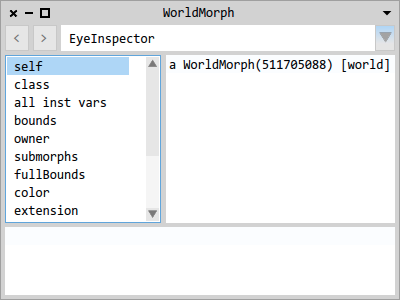
\includegraphics[scale=0.5]{inspector-view-default}
		\caption{}
	\end{subfigure}\\
	\vspace{\baselineskip}
	\begin{subfigure}[t]{\textwidth}
		\centering
		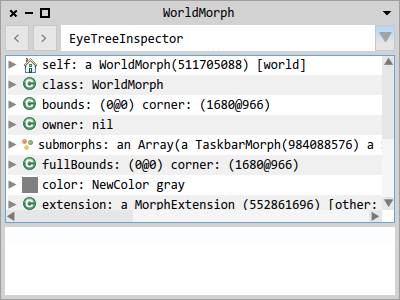
\includegraphics[scale=0.5]{inspector-view-tree}
		\caption{}
	\end{subfigure} 

	\caption[Default Inspectors Views]{}
\end{figure}

\begin{figure}[h]
	\centering
	\begin{subfigure}[b]{\textwidth}
		\centering
		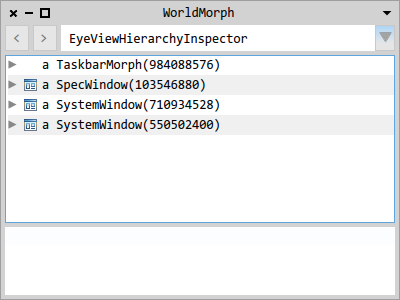
\includegraphics[scale=0.5]{inspector-view-submorphs}
		\caption{.}
	\end{subfigure}\\
	\vspace{\baselineskip}
	\begin{subfigure}[b]{\textwidth}
		\centering
		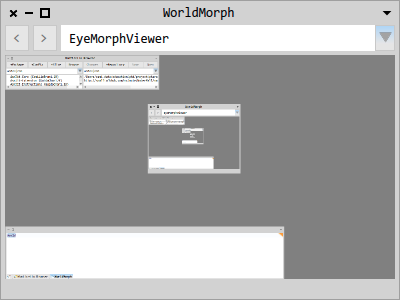
\includegraphics[scale=0.5]{inspector-view-morph}
		\caption{.}
	\end{subfigure}
	
	\caption[Morph Specific Inspector Views]{}
\end{figure}

% ---------------------------------------------------------------------------
\subsection{Inspector Applications}
% ---------------------------------------------------------------------------
\todo{Specific Inspector Picture: Morph} \\
\todo{Specific Inspector Picture: Mate Stack Inspector} \\
\todo{Minor vision on an inspector-based Environment}

% =============================================================================
\section{First-class Object Layouts: Bridging the Gap to the Memory}
% =============================================================================
\todo{Introduction: Smalltalk Objects -> missing reification -> wrapper apps instead (Magritte)}

% ---------------------------------------------------------------------------
\subsection{Objects All the Way}
% ---------------------------------------------------------------------------


% ---------------------------------------------------------------------------
\subsection{Layouts and Slots}
% ---------------------------------------------------------------------------
\todo{Copy most of the pictures from the Slot Paper}

% ---------------------------------------------------------------------------
\subsection{Future Applications}
% ---------------------------------------------------------------------------
\todo{Reified Object Relationships} \\
\todo{Optimizations: Bitfields, HashVars} \\
\todo{DB/Meta Mapping: Magritte on classes} \\
\todo{Spec}

% =============================================================================
\section{Related Work}
% =============================================================================

% -----------------------------------------------------------------------------
\subsection{Meta Object Protocols}
% -----------------------------------------------------------------------------
\todo{Kiczales \cite{Kicz91a}} \\
\todo{List Smalltalk MOP} \\
\todo{Link back to the Slots as Memory MOP} \\
\todo{more?}

% -----------------------------------------------------------------------------
\subsection{VM Hooks}
% -----------------------------------------------------------------------------
\todo{Link from previous subsection with DNU hook} \\
\todo{Efficient Method Lookup Customization: \cite{Vran12a}} \\
\todo{Meta-Crossing Method Lookup in Pinocchio} \\	
\todo{more?}

% =============================================================================
\section{Summary}
% =============================================================================


% =============================================================================
\ifx\wholebook\relax\else
    \end{document}
\fi
% =============================================================================
\documentclass[a4paper,12pt,twoside]{../includes/ThesisStyle}
\usepackage[utf8]{inputenc}
\usepackage[T1]{fontenc}

\usepackage[left=1.5in,right=1.3in,top=1.1in,bottom=1.1in,includefoot,includehead,headheight=13.6pt]{geometry}\renewcommand{\baselinestretch}{1.05}


% =============================================================================
%\usepackage[sectionbib]{chapterbib}	% Cross-reference package (Natural BiB)
%\usepackage{bibunits}
%\usepackage{natbib}					% Put References at the end of each chapter
\usepackage{algorithm}
\usepackage{alltt}
\usepackage{amsfonts}
\usepackage{amsmath}
\usepackage{amssymb}
\usepackage{cite}
\usepackage{color}
\usepackage{enumerate}
\usepackage{booktabs} % used for \midrule
\usepackage{fancyhdr}					% Fancy Header and Footer
\usepackage{graphicx}
\usepackage{ifthen}
\usepackage{latexsym}
\usepackage{multirow}
\usepackage{rotating}					% Sideways of figures & tables
\usepackage{stmaryrd}
\usepackage{subfigure}
\usepackage{url}         
\usepackage{xspace}
\usepackage[normalem]{ulem} % for \sout
\usepackage{xcolor}
\usepackage{tablefootnote}
\usepackage{pifont}

% =============================================================================

% Table of contents for each chapter
\usepackage[nottoc, notlof, notlot]{tocbibind}
\usepackage{minitoc}
\setcounter{minitocdepth}{1}
\mtcindent=15pt

\setcounter{secnumdepth}{3}
\setcounter{tocdepth}{2}
  
% =============================================================================
% Fancy Header Style Options

\pagestyle{fancy}                       % Sets fancy header and footer
\fancyfoot{}                            % Delete current footer settings

%\renewcommand{\chaptermark}[1]{         % Lower Case Chapter marker style
%  \markboth{\chaptername\ \thechapter.\ #1}}{}} %

%\renewcommand{\sectionmark}[1]{         % Lower case Section marker style
%  \markright{\thesection.\ #1}}         %

\fancyhead[LE,RO]{\bfseries\thepage}    % Page number (boldface) in left on even
% pages and right on odd pages
\fancyhead[RE]{\bfseries\nouppercase{\leftmark}}      % Chapter in the right on even pages
\fancyhead[LO]{\bfseries\nouppercase{\rightmark}}     % Section in the left on odd pages

\let\headruleORIG\headrule
\renewcommand{\headrule}{\color{black} \headruleORIG}
\renewcommand{\headrulewidth}{1.0pt}
\usepackage{colortbl}
\arrayrulecolor{black}

\fancypagestyle{plain}{
  \fancyhead{}
  \fancyfoot{}
  \renewcommand{\headrulewidth}{0pt}
}


% =============================================================================
% Clear Header Style on the Last Empty Odd pages
\makeatletter

\def\cleardoublepage{\clearpage\if@twoside \ifodd\c@page\else%
  \hbox{}%
  \thispagestyle{empty}%              % Empty header styles
  \newpage%
  \if@twocolumn\hbox{}\newpage\fi\fi\fi}

\makeatother

\newenvironment{maxime}[1]
{
\vspace*{0cm}
\hfill
\begin{minipage}{0.5\textwidth}%
%\rule[0.5ex]{\textwidth}{0.1mm}\\%
\hrulefill $\:$ {\bf #1}\\
%\vspace*{-0.25cm}
\it 
}%
{%

\hrulefill
\vspace*{0.5cm}%
\end{minipage}
}

\let\minitocORIG\minitoc
\renewcommand{\minitoc}{\minitocORIG \vspace{1.5em}}


\renewcommand{\epsilon}{\varepsilon}

% centered page environment
\newenvironment{vcenterpage}
	{\newpage\vspace*{\fill}\thispagestyle{empty}\renewcommand{\headrulewidth}{0pt}}
	{\vspace*{\fill}}
	

%=============================================================================

\usepackage{needspace}
\newcommand{\needlines}[1]{\Needspace{#1\baselineskip}}

\usepackage{xcolor}
\definecolor{source}{gray}{0.95}
% source code formatting
\usepackage{listings}
    % global settings for source code listing package
\lstset{
    basicstyle=\ttfamily\small,
    showspaces=false,
    showstringspaces=false,
    captionpos=b, 
    columns=fullflexible}

\lstdefinelanguage{ST}{
    keywordsprefix=\#,
    morekeywords=[0]{true,false,nil},
    morekeywords=[1]{self,super,thisContext},
    morekeywords=[2]{ifTrue:,ifFalse:,whileTrue:,whileFalse:,and:,or:,xor:,not:,by:,timesRepeat:},
    sensitive=true,
    morecomment=[s]{"}{"},
    morestring=[d]',
    escapechar={!},
    alsoletter={., :, -, =, +, <},
    moredelim=**[is][\itshape]{/+}{+/},
    literate=
        {^}{{$\uparrow$}}1
        {:=}{{$\leftarrow$}}1
        {~}{{$\sim$}}1
        {-}{{\sf -\hspace{-0.13em}-}}1  % the goal is to make - the same width as +
        {+}{\raisebox{0.08ex}{+}}1		% and to raise + off the baseline to match V
        , % Don't forget the comma at the end!
    style=STStyle
}
\lstdefinestyle{STStyle}{
    tabsize=4,
    %frame=leftline,
    % frame=bl,
    %framerule=2pt,
    %rulecolor=\color{gray},
    % backgroundcolor=\color{white},
    %backgroundcolor=\usebeamercolor[bg]{listing},
    basicstyle=\ttfamily\small,
    keywordstyle=\bf\ttfamily,
    % stringstyle=\color{orange},
    stringstyle=\mdseries\slshape,
    commentstyle=\it\rmfamily\color{darkgray}, 
    commentstyle=\mdseries\slshape\color{gray},
    %commentstyle=\mdseries\slshape,
    emphstyle=\bf\ttfamily,
    escapeinside={!}{!},
	%backgroundcolor=\color{source},
    %emphstyle={[2]\color{red}},
    %emphstyle={[3]\color{blue}\bf},
    %emphstyle={[4]\color{blue}},
    keepspaces=true
} 

%\lstnewenvironment{javacode}  [1][]{\lstset{language=java,#1}\needlines{#2}}{} 
%\lstnewenvironment{pythoncode}[2][]{\lstset{language=python,#1}\needlines{#2}}{}
\lstnewenvironment{stcode}    [2][]{\lstset{language=ST,#1}\needlines{#2}}{}
\lstnewenvironment{ccode}     [2][]
    {\lstset{language=C,numbers=left,escapechar=\$,numberstyle=\tiny,#1}\needlines{#2}}{}

% ON: I tried to pass the line number options in as arg #1 but it does not work for me
% I also could net get the line numbers to consistently increase
\lstnewenvironment{numstcode} [2][]
    {\lstset{language=ST,numbers=left,numberstyle=\tiny,numbersep=2pt,#1}\needlines{#2}}{}
\lstnewenvironment{numstcodecont} [2][]
    {\lstset{language=ST,numbers=left,numberstyle=\tiny,numbersep=2pt,firstnumber=last#1}\needlines{#2}}{}

\newcommand{\lst}[1]{{\tt #1}}

% In-line code (literal)

% In-line code (latex enabled)
% Use this only in special situations where \ct does not work
% (within Section headings ...):
\newcommand{\lct}[1]{{\textsf{\textup{#1}}}}
% Code environments
\lstnewenvironment{code}{%
	\lstset{%
		% frame=lines,
		frame=single,
		framerule=0pt,
		mathescape=false
	}
}{}

%\renewcommand{\lstlistingname}{Code Example}

% =============================================================================
\newboolean{showcomments}
\setboolean{showcomments}{true}

\ifthenelse{\boolean{showcomments}} {
	\newcommand{\ugh}[1] {\textcolor{red}{\uwave{#1}}}	% please rephrase
	\newcommand{\ins}[1] {\textcolor{blue}{\uline{#1}}}	% please insert
	\newcommand{\del}[1] {\textcolor{red}{\sout{#1}}}	% please delete
	\newcommand{\chg}[2] {								% please change
		\textcolor{red}{\sout{#1}}{\ra}
		\textcolor{blue}{\uline{#2}}}
	\newcommand{\nbc}[3]{								% comment
		{\colorbox{#3}{\bfseries\sffamily\scriptsize\textcolor{white}{#1}}}
		{\textcolor{#3}{\sf\small$\blacktriangleright$\textit{#2}$\blacktriangleleft$}}}

}{
	\newcommand{\ugh}[1]{#1}							% please rephrase
	\newcommand{\ins}[1]{#1}							% please insert
	\newcommand{\del}[1]{}								% please delete
	\newcommand{\chg}[2]{#2}							% please change
	\newcommand{\nbc}[3]{}								% comment
}

% =============================================================================
\usepackage[pagebackref,hyperindex=true]{hyperref}


% Links in pdf
\usepackage{color}
\definecolor{linkcol}{rgb}{0.0, 0.0, 0.0} 
\definecolor{citecol}{rgb}{0.0, 0.0, 0.0} 

% Change this to change the informations included in the pdf file
% See hyperref documentation for information on those parameters
\hypersetup {
	bookmarksopen=true,
	pdftitle="Design and Use of Anatomical Atlases for Radiotherapy",
	pdfauthor="Olivier COMMOWICK", 
	pdfsubject="Creation of atlases and atlas based segmentation", %subject of the document
	%pdftoolbar=false, % toolbar hidden
	pdfmenubar=true, %menubar shown
	pdfhighlight=/O, %effect of clicking on a link
	colorlinks=true,
	pdfpagemode=UseNone,
	pdfpagelayout=SinglePage,
	pdffitwindow=true,
	linkcolor=linkcol,
	citecolor=citecol,
	urlcolor=linkcol
}

% =============================================================================
\newcommand{\figlabel}[1] {\label{fig:#1}}
\newcommand{\chaplabel}[1]{\label{chap:#1}}
\newcommand{\seclabel}[1] {\label{sec:#1}}
\newcommand{\tablabel}[1] {\label{tab:#1}}
\newcommand{\lstlabel}[1] {\label{lst:#1}}

\newcommand{\figref}[1] {Figure~\ref{fig:#1}}
\newcommand{\chapref}[1]{Chapter~\ref{sec:#1}}
\newcommand{\secref}[1] {Section~\ref{sec:#1}}
\newcommand{\tabref}[1] {Table~\ref{tab:#1}}
\newcommand{\lstref}[1] {Listing~\ref{tab:#1}}

\newcommand{\commented}[1]{}

\newcommand{\bs}    {\symbol{'134}} % backslash
\newcommand{\us}    {\symbol{'137}} % underscore
\newcommand{\ttt}[1]{\texttt{#1}}
\newcommand{\ie}    {\emph{i.e.},\xspace}
\newcommand{\eg}    {\emph{e.g.},\xspace}
\newcommand{\etal}  {\emph{et al.}\xspace}
\newcommand{\ns}    {\!\!\!\!} %big negative space
\newcommand{\cnull} {\textbackslash0\xspace}


\newcommand\fix[1]{\nb{FIX}{#1}}
\newcommand\todo[1]{\nb{TO DO}{#1}}
\newcommand\cb[1]{\nbc{CB}{#1}{purple}}
\newcommand\sd[1]{\nbc{SD}{#1}{orange}}
\newcommand\is[1]{\nbc{IS}{#1}{gray}}
\newcommand\gc[1]{\nbc{GC}{#1}{olive}}
\newcommand\ct[1]{\nbc{CT}{#1}{teal}}
\newcommand\md[1]{\nbc{MD}{#1}{blue}}
\newcommand\dc[1]{\nbc{DC}{#1}{green}}

% =============================================================================
\newcommand{\NBFFI}  {Native\-Boost-FFI\xspace}
\newcommand{\NB}  {Native\-Boost\xspace}
\newcommand{\B}   {Benzo\xspace}
\newcommand{\ST}  {Small\-talk\xspace}
\newcommand{\PH}  {Pharo\xspace}
\graphicspath{{.}{../figures/}}

\begin{document}
% =============================================================================

\chapter{Benzo}
\chaplabel{benzo}
\minitoc

% =============================================================================

% ===========================================================================
\section{Introduction}
\seclabel{benzo-introduction}
% ===========================================================================
\todo{Write thesis introduction, the current introduction is more background / motivation}

% ===========================================================================
\section{Background}
\seclabel{benzo-background}
% ===========================================================================
High-level low-level programming \cite{Fram09a} encourages to use high-level languages such as Java to build low-level execution infrastructures or to do system programming. 
It is successfully used in experimental high-level self-hosted virtual machines (VMs) such as Jikes~\cite{Alpe99a}.  
Frampton et al. present a framework that is biased towards a statically typed high-level language, taking strict security aspects into account.
Their approach promotes to address low-level system programming tasks with the tools and abstractions of high-level languages.
However, their solution has reduced applicability in a dynamic and reflective context.
By reflective, we refer to the combined capabilities to inspect (introspection) and change (intercession) the same execution concepts at runtime \cite{Maes87a}.

From a reflective point of view it seems natural to dynamically modify the VM at runtime and not just at compile-time.
If we are able to modify the VM from language-side we blur the line between these two distinct worlds, becoming indistinguishable to talk about the VM or the language-side.
Hence throughout this paper we use the term language runtime to refer to the running VM combined with the language-side application.


%Extending high-level language VM is difficult due to their static low-level construction which usually shares little resemblance with the language-side.
%Yet for tasks, like the previously presented primitive instrumentation, if we want to tackle it with a high-level language, we need solid low-level interaction.
%\cb{some more context missing here}

\subsection{Requirements.}
Extending the VM is only one particular case of modifying or extending the complete language runtime.
Language-side libraries, reflective capabilities, VM extensions or hybrid approaches are other possibilities which we discuss in detail in Section~\secref{related}.
All these typical extension mechanisms are not sufficient if we want to modify the VM from language-side, or in our terminology, to reflectively modify the language runtime. Furthermore these mechanisms are based on the fact that there is a clear barrier between language and VM.
A solution that crosses these barriers requires the following properties:

%interface to interact with low-level code.
%To stay flexible and compatible enough a generic solution should add these new key features with as little static low-level intrusion as possible.

\begin{enumerate}
	\item It must be \emph{reflective} in the sense it must support \emph{dynamic} changes of the language runtime (VM) without requiring a system restart.
	\item It should imply minimal changes to the existing low-level runtime to \emph{considerably reduce development efforts}.
\end{enumerate}


\subsection{\B a Framework for Reflective Low-level Programming.}

High-level low-level programming is a powerful technique for system programming without resorting to static low-level environments \cite{Fram09a,Wimm13a} that \ugh{almost} fulfills our requirements.
However, in a reflective setup it fails to comply with the first requirement mentioned in the previous paragraph: it does not allow reflective changes at runtime.
Our approach for overcoming this limtation consists of \B, a lightweight and reflective framework that dynamically generates native code from language-side and allows its execution on the fly.
It relies only on a small set of generic VM extensions described in Section~\secref{vm-requirements}, whereas the vast majority of the framework is implemented as a language-side library.

\subsection{\B Applications.}
In Section \secref{usecase} we advocate the contribution of this approach by providing three different incremental examples that heavily use the framework.
Unlike typical implementations that would focus on writing them as VM extensions, we implement them completely at language-side using \B:
%\ugh{They rely on it} for extending or even improving language runtime capabilities.

%\begin{description}[noitemsep]
\begin{description}
	\item[FFI] A complete language-side Foreign Function Interface (FFI) implementation, described in Section \secref{ffi}.
	\item[Dynamic Primitives] A language-side compilation toolchain that replaces system primitives at runtime with customized code, described in Section \secref{waterfall}. 
	\item[Language-side JIT Compiler] A JIT compiler that works at language-side and interacts with the VM for code synchronization, described in Section \secref{nabujito}
\end{description}


\noindent Illustrated by these three distinct examples, the contributions of this paper are:
\begin{enumerate} 
	\item A \emph{reflective} high-level low-level programming framework that encourages the extension of high-level language runtimes on the fly without the overheads imposed by pure high-level solutions. 
	%\item The framework promotes open interactions with the low-level world .
	\item A proof of concept of the proposal with the implementation and description of three different tools that heavily use reflective low-level programming and covers distinct scenarios.
\end{enumerate}


%\subsection{Use Case: Dynamic Primitive Instrumentation}
%\md{Remove use-case here and inline in 1.2 Bridging abstraction layers}
%\noindent To illustrate this limitation we take the example of dynamically intercepting VM primitives. In most managed language runtimes, VM primitives are used for essential tasks such as object creation or provide fundamental functionality that can not be obtained otherwise at language-side~\cite[page 52]{Gold83a}. Already the simple example of measuring the time spent in an essential primitive while executing a performance critical task is difficult to do efficiently.


%Reflective solutions at language-side could take advantage of the intercession capabilities that allow changing or augmenting almost any behavior at runtime. In practice, this does not work for primitives. In addition, reflectively measuring the duration of the time primitive itself will easily cause meta-recursion. Hence in general reflective instrumentation will not work on primitives used for the instrumentation itself. Thus efficiently instrumenting VM primitives in a dynamic and reflective environment is not feasible in many cases.

%Naturally, if we leave the high-level realm there are efficient tools at hand for instrumentation. Existing solutions for efficient low-level instrumentation such as DTrace~\cite{Coop12a} work by installing static hooks. Though in a reflective language assumptions can change at runtime and thus static solutions are not appropriate. At the same time we clearly see that such instrumentation is not a typical high-level application. To combine these two worlds we need a different approach.


% ===========================================================================
\section{The \B Framework}
\seclabel{benzo}
% ===========================================================================
\B is implemented in \PH\footnote{\url{http://pharo.org}}, a \ST inspired language.
\PH comes with all the reflective capabilities known from \ST where most language-side components can be altered dynamically.
\B is implemented at language-side and only requires the help of two simple and generic primitives to activate \cb{ad-hoc has a negative conotation} native code and resolve the entry point address position of referenced C functions.

%----------------------------------------------------------------------------
\subsection{VM Context}
\seclabel{vm-requirements}
%----------------------------------------------------------------------------
\PH emerged from the Squeak project \cite{Inga97a}.
The \PH VM (Cog) implementation \cite{Mira11a} also evolved from the original Squeak bytecode interpreter.
The current VM uses a moving Garbage Collector (GC) with two generations\gc{ref?} and uses a JIT that applies basic register allocation to reduce stack load. 
This situation is not a direct requirement for \B but it is assumed as given and thus not further discussed in detail.
However, \B requires certain features that were not supported in the existing VM implementation.
Mainly our requirement is being able to generate executable code and activate it at runtime.
This is general and essential so it applies to any VM that wants to support dynamic code execution managed at language-side.

%----------------------------------------------------------------------------
\paragraph{Executable Memory.}
\seclabel{exeutable-memory}
 
We use standard \ST objects to hold the generated native code.
However, by default the object memory is not executable.
This leaves two choices: mark the whole object memory executable or only move the objects with the native code to a special executable memory region.
We took the path of least resistance and marked the whole object memory as executable.
The other solution requires substantial changes for memory management. As the VM has a moving GC we only access high-level \ST objects via an indirection from low-level code.
Another approach would have been to harness the fixed sized executable region used by the existing JIT.
However, the JIT space does not hold normal \ST objects but special low-level structures and uses its own special GC. 

%----------------------------------------------------------------------------
\paragraph{VM Interaction.}
\seclabel{vm-interaction}

\todo{dig up the older versions of this section with the longer text}

The standard way in \ST to execute low-level code is to use a tag in the method definition. The following example shows such a method on the \ttt{Float} class.
%
\begin{stcode}[label={lst:basic-primitive}]{5}
* aNumber 
	<primitive: 49>
	^ aNumber adaptToFloat: self andSend: #*
\end{stcode}
%
Here we use the primitive 49 to call a VM function which efficiently multiplies two floats. 
Figure~\figref{smalltalkPrimitive}-a describes the case where the primitive is successfully executed.
However, if the primitive is unable to do the operation, for instance if the argument \ttt{aNumber} is not a float, it will signal a failure which causes the VM to execute the fallback \ST code in the method body.  
Fig.~\figref{smalltalkPrimitive}-b describes it. 

\begin{figure}[ht]
	\centering
	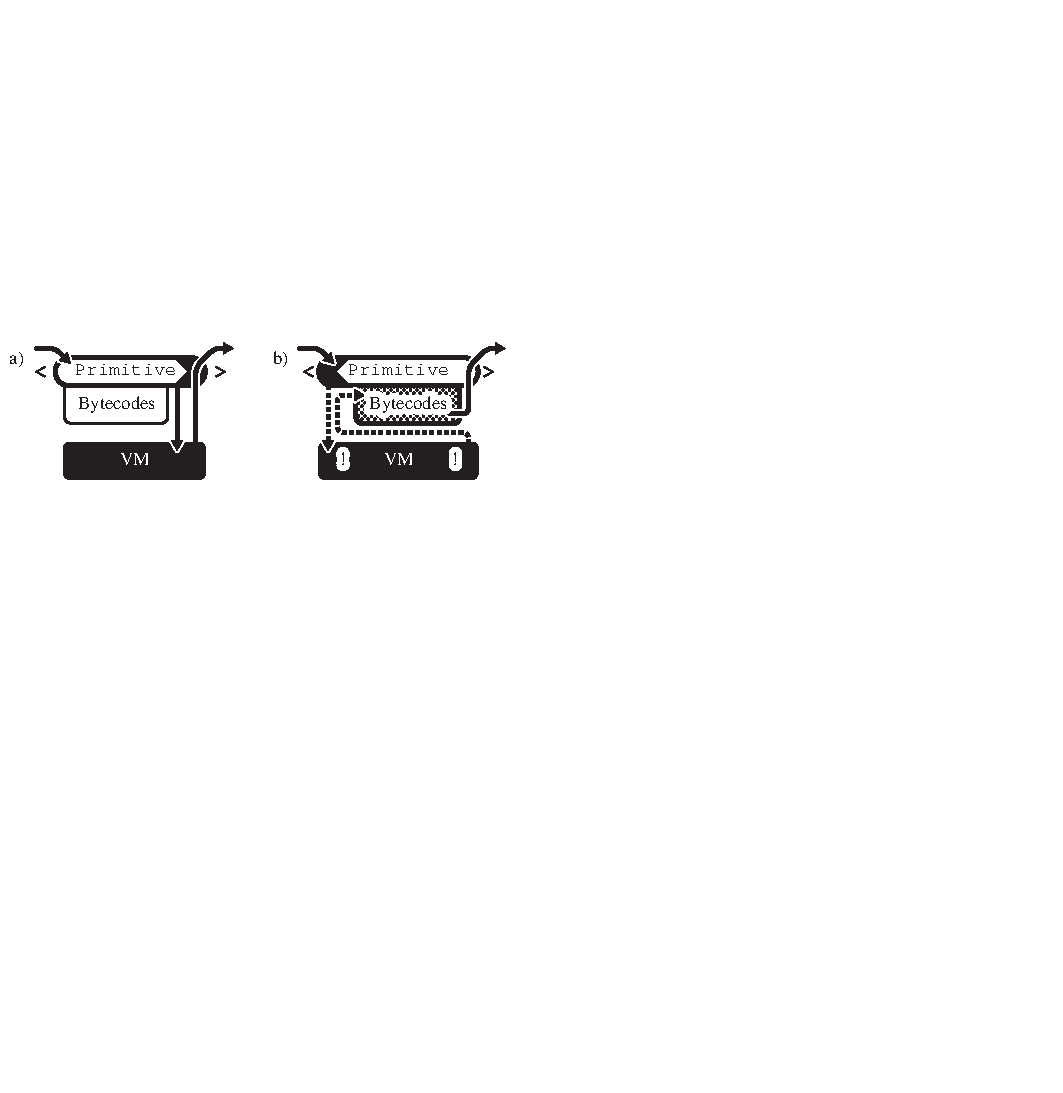
\includegraphics[scale=1.1]{smalltalkPrimitive}
	%\nocaptionrule
	\caption{Generic primitive methods in \PH: a) A primitive completely bypasses the bytecode, b) A failing primitive executes the \ST bytecode as fallback.}
	\figlabel{smalltalkPrimitive}
\end{figure}


\B uses the primitives as a gate to enter the low-level world from the language-side.
Our custom primitive then executes the generated native code and returns to language-side. 
This code is appended inside the compiled method object.
When the primitive is activated, it  accesses the currently executed compiled method via a VM function. Figure \figref{nativeCodeMethod} shows the structure of a \ST compiled method that has native code attached to it.
We see the primitive tag on top, followed by the literal frame which holds references to symbols and classes used in the method.
The subsequent \ST bytecode is the fallback code executed only if the primitive fails. Only then appears the native instructions.
A marker at the end of the compiled method called trailer type is used to flag methods that actually have native code attached to them.
%
\begin{figure}[ht]
	\centering
	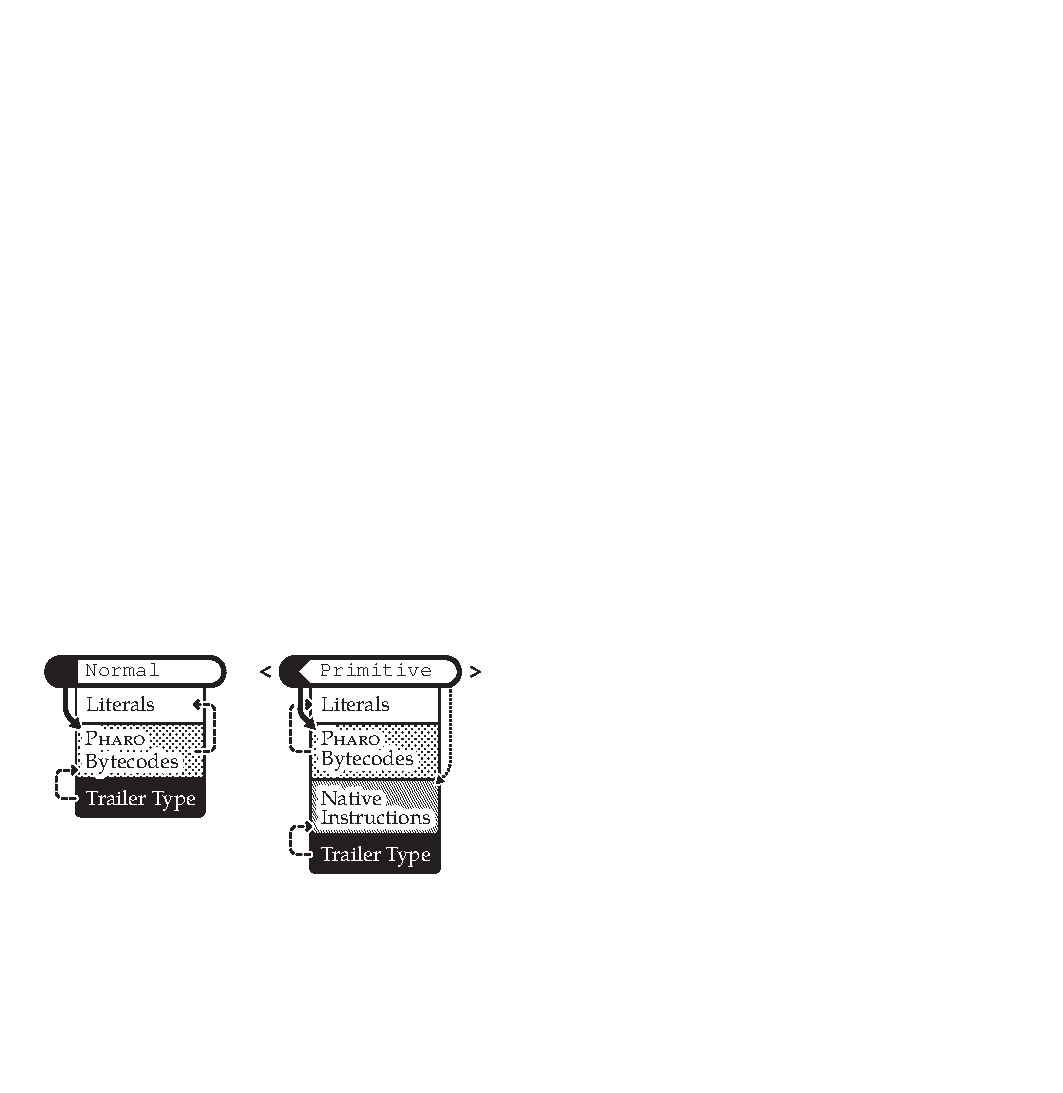
\includegraphics[scale=1.1]{nativeCodeMethod}
	%\nocaptionrule
	\caption{A standard \ST compiled method on the left and a method with appended native instructions generated by \B.}
	\figlabel{nativeCodeMethod}
\end{figure}

Since compiled methods are first-class objects it is possible to modify them at runtime and append the native code.
The primitive \ttt{primitiveNativeCall}, which is implemented by \B, is the responsible of running the native instructions in a \ST method.
The code example \ttt{interrupt3} shows a very basic application of our infrastructure.
In Section \secref{benzo-language-side}, through more detailed examples, we describe how \B uses \ST code to generate the native instructions.
%
\begin{stcode}[label={lst:basic-native-code}, caption={\ST method using \B for very basic low-level debugging.}, escapeinside={@}{@}]{5}
interrupt3
	<primitive: 'primitiveNativeCall' 
	 module: 'BenzoPlugin' >
	Benzo generate: [ :asm | asm int3 ]
\end{stcode}

%----------------------------------------------------------------------------
\paragraph{Native Code Platform Interaction.}
\seclabel{platform-interaction}

To ensure that the code is compatible with the current platform a VM specific marker is expected at the beginning of the native code on the compiled method.
Upon activation \B compares this marker with the one from the current VM.
If they don't match, \B signals a failure that causes the VM to evaluate the fallback \ST code.
With this elegant approach \B regenerates native code lazily on new platforms.
Moreover, it does not have to flush the native code when the application is restarted on the same platform.

%----------------------------------------------------------------------------
\paragraph{Garbage Collector Interaction.}
\seclabel{gc-interaction}
\todo{dig up the older versions of this section with the longer text}

Compiled methods in \PH have a special section, the literal frame, which stores objects referenced in the bytecodes.
Bytecodes then only have indirect access to these objects by indexing into the literal frame.
This simplifies the implementation of the garbage collector as it only has to scan the beginning of each method for possible references to objects. 
So the GC only tracks \ST objects when they are in the method literal frame. 
The moving GC of the VM used for \PH has a significant impact on the low-level code we can generate using \B.
For instance it is not possible to statically refer to language-side objects from native code as object addresses change after each garbage collection.
Modifying the GC to support regions of non-moving objects would solve this problem.
However, we chose to minimize the number of low-level VM modification necessary to run our experiments and opted for a simpler solution.
\B accesses language-side objects through an indirection.
For indirectly accessing objects the Pharo VM already features a special structure, named \emph{external roots}.
This array has a fixed-location in memory which can be used to access moving language-side objects.
The GC updates the addresses in this VM structure after each run.
Hence we have the static address of the external roots object as an entry point to statically access \ST objects.
%
\begin{figure}[ht]
	\centering
	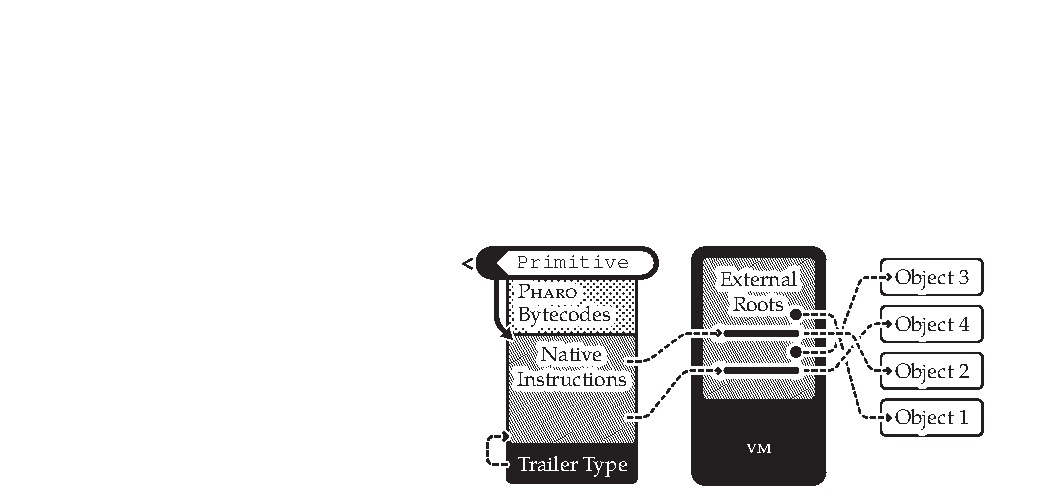
\includegraphics[scale=1.1]{externalRoots}
	%\nocaptionrule
	\caption{Pointers to objects registered as external roots are pinpointed at fixed offset in global VM-level object.
	}
	\figlabel{externalRoots}
\end{figure}
%
Summarizing, for accessing \ST objects within native code we first register it as an external root object and access it only indirectly.
This means that for native code, instead of a method-local literal array we share a global literal array as shown in Figure \figref{externalRoots}. 
\B only adds an \ttt{Array} to the external root objects which is managed from language-side and administers all references.

%\revc{The external roots concept appears here first but the idea of "indirection" has been mentioned. The regular literal frame of compiled methods are discussed heavily; that would suggest that the generated native code could use relative offset from the code location and still be able to "pin-point" the literal slot in the literal frame. What is the downside of this approach? (And how slots in the external roots garbage collected?)}
%\gc{I'm not very interested with the comment above. But perhaps here it is a good place to say that once the native code start executing our VM assures that a GC could not happen}
%----------------------------------------------------------------------------
\paragraph{JIT Interaction.}
\seclabel{jit-interaction}

When the Pharo VM starts the execution of dynamic generated code the execution environment changes slightly.
Similarly, when entering primitives or plugin code, the managed execution mode is left and a normal C-level execution environment is reestablished until the primitive finishes and the VM jumps back to the jitted code. 
To avoid these context changes that imply a considerable performance overhead, we extend the VM to support inlining of native code in the JIT phase following the same strategy as other existing primitives which are inlined at JIT-level.
The \B prologue and epilogue used for managing the low-level stack are replaced by an adapted version for the JIT.
The performance boost of this optimization is further discussed in Section \secref{issues-performance}.

%----------------------------------------------------------------------------
\paragraph{Error Handling.}
\seclabel{error-handling}

\todo{extend with an explicit example}

\B provides an error handling facility that allows to return high-level error messages from the low-level code. 
The native code builder provides a helper method called \ttt{failWithMessage:} 
that generates the proper assembler instructions to return a full error message.
This allows plugins to return clear and meaningful error codes, improving the debugging tasks and enabling a better interaction with users.

%\reve{does a call to "failWithMessage:" result in an exception being thrown, or does it just display an error message. The former would be more useful b/c it would enable language-side code to catch the exception and do something about it, but the paper doesn't make it clear that this is the case.}


%----------------------------------------------------------------------------
\subsection{\B's Language-Side Implementation}
\seclabel{benzo-language-side}
%----------------------------------------------------------------------------
As a key design decision, we determine to keep the interface to the low-level world minimal.
The following describes the features of \B at the high-level language-side.

%----------------------------------------------------------------------------
\paragraph{Code Generation.}
\seclabel{code-generation}

\B delegates native code generation to a full assembler written in \ST. The following example shows how to use the assembler to generate the native code for moving \ttt{1} into the 32-bit register \ttt{EAX}.
%
\begin{stcode}{4}
Benzo x86 generate: [ :asm |
	asm mov: 1 asUImm to: asm EAX ].
\end{stcode}
%
The implementation first creates a slightly more abstract intermediate format.
The abstract operations can be extended by custom operations that may expand to several native instructions. For pragmatic reasons current implementation only supports \textsc{x86} and \textsc{x86-64}.
%
%	\reve{You claim that the "assembler is platform-agnostic", but how so? In the examples, you seem to use instructions that are clearly x86-specific, e.g., MOVs involving EAX. On a related note, you say in the same section that "there are plans to improve the platform independence by implementing a more abstract DSL for NativeBoost."}
%
The full features of the high-level environment are available when generating native code.
Hence complex instruction sequences can easily be delegated to other objects.
In the following example we use a VM helper to instantiate an array. It is worth noting that all are standard message sends:
%
\begin{stcode}{5}
Benzo x86 generate: [ :asm :helper | | register |
	register := helper classArray.
	register := helper 
		instantiateClass: register
		indexableSize: 10
	asm mov: register to: asm resultRegister ].
\end{stcode}
%
The VM helper exposes a basic, low-level interface to access objects and its properties.
Additional methods cover the access to the external roots described in Section \secref{gc-interaction}.
In this case the \ttt{\#instantiateClass:indexableSize:} will generate the proper native code to call to a VM function and make sure that the side-effects of a possible GC run are handled properly.
By default the value in the result register is returned back to the language-side. On \textsc{x86} this defaults to \ttt{EAX}.
In section \secref{usecase} we introduce more substantial applications based on \B.

%----------------------------------------------------------------------------
\paragraph{Code Activation.}
\seclabel{code-activation}
 
A \B primitive is responsible for the native code activation which consists of three main steps:
%
%\begin{itemize}[noitemsep,nolistsep] 
\begin{enumerate}
	\item Check if there is native code in the actual compiled method and if it is compatible with the current platform.
	\item Generate native code if necessary.
	\item Activate the native code for execution.
\end{enumerate}
%
The example in Listing \lstref{basic-native-code} uses \B's generator to create and install the native code which would trigger a low-level interrupt. Behind the scenes \B adds some more information to the code as the already mentioned platform marker. 
For activation \B uses reflective features to restart the method containing the native code.
Upon the second activation, after already generating the native code, \B moves the native code to the end of the compiled method and activates it.
This mechanism is shown in Figure \figref{nativeCodeActivation}.

\begin{figure}[ht]
	\centering
	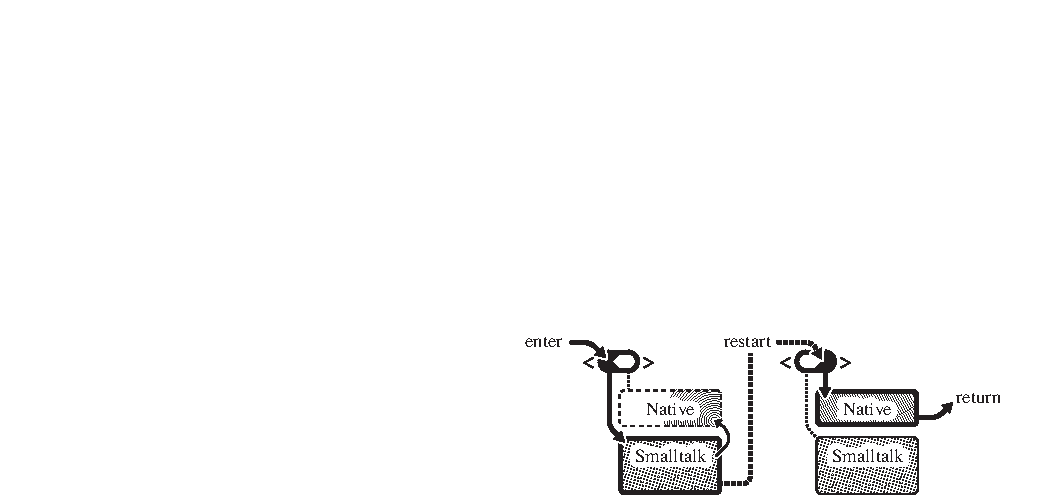
\includegraphics[scale=1.1]{nativeCodeActivation}
	\caption{Native code activation with \B: The first call triggers the code generation. Then the method is restarted and the native code executed.}
	\figlabel{nativeCodeActivation}
\end{figure}

% ===========================================================================
\section{\B in Practice}
\seclabel{usecase}
% ===========================================================================
\todo{keep this section as is and introduce forward pointers to the separate chapters}

In this Section, for illustrating better the contribution of the solution proposed, we will present different dynamic language-side applications and tools based on \B.
%These implementations, a FFI, dynamic primitives and a language-side JIT, are typically done at VM-level.
%We show that \B is a competitive solution.

%----------------------------------------------------------------------------
\subsection{\NB: \B-based Foreign Function Interface}
\seclabel{ffi}
%----------------------------------------------------------------------------

%\begin{figure*}[t]
%\centering
%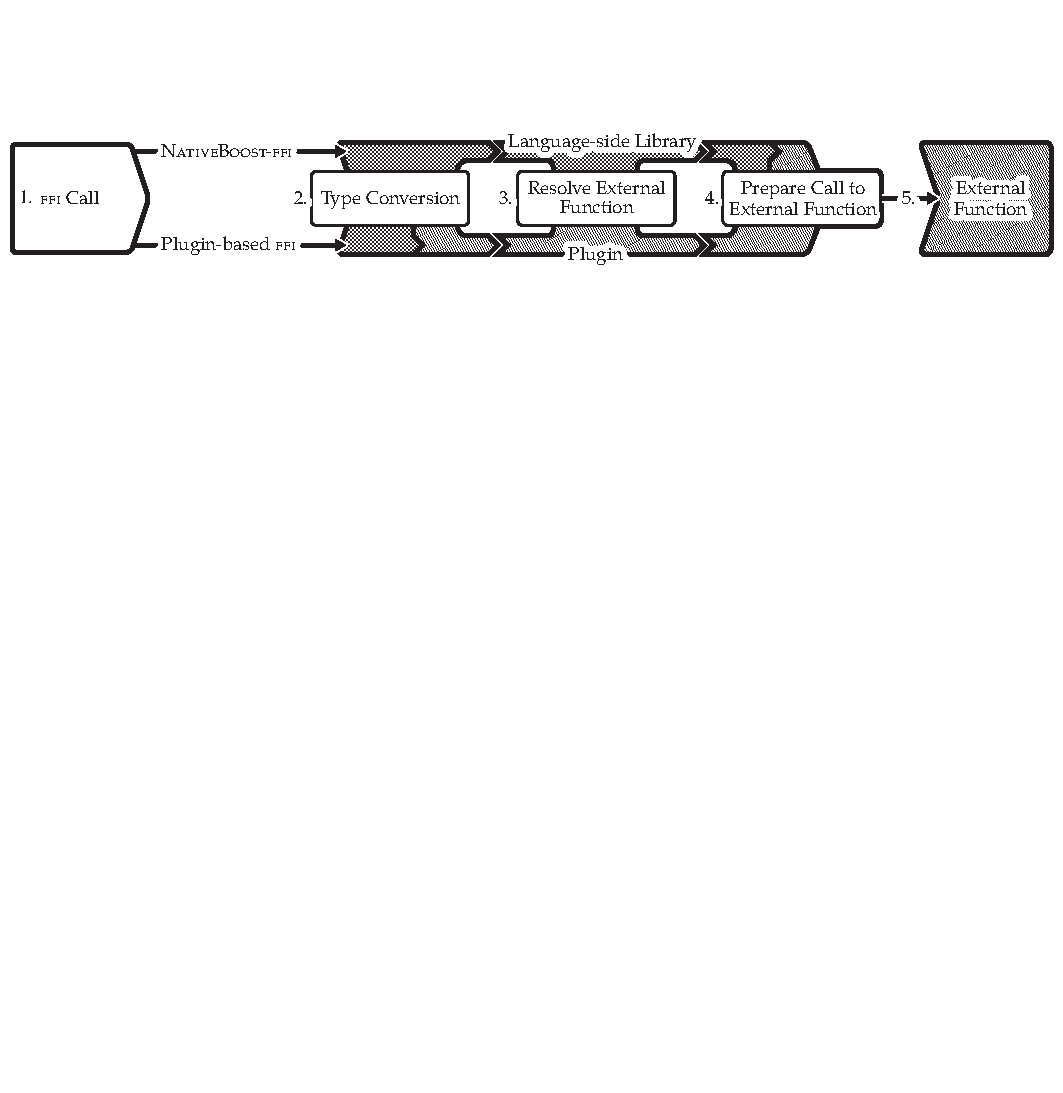
\includegraphics[width=\linewidth]{ffiOverview}
%\caption{\NB Overview: Unlike typical FFI implementations \NB only resorts to the VM-level when actually calling the external function in step 4. Typical implementations already cross the low-level barrier during the type conversions at step 2.}
%\figlabel{ffi}
%\end{figure*}

FFIs enable a programmer to call external functions without the need to implement additional VM extensions.
\NB \cite{Brun13a} is a production-ready FFI for \PH, developed on top of \B.
An FFI implementation consists of two main parts: calling external functions and converting data between the two environments.
Typically a big percentage of these two parts are implemented at VM-level with statically defined bindings.
Relying on \B's capability to dynamically generate and execute native code we developed a complete FFI at language-side.
This way the VM no longer requires to have a specific FFI extension.

%----------------------------------------------------------------------------
%\paragraph{FFI at Language-side.} 
%
%The fact that via FFI we can call external functions makes it a perfect option to replace VM extensions defined at low-level side since FFI relies only on one generic low-level extension: the language-side has to be able to generate and subsequently call native instructions. 
%A VM with a well-defined plugin infrastructure enforces the same level of separation.
%However, unlike plugins, FFI bindings are implemented without crossing a language barrier. 
%Most code for FFI bindings can be written at language-side in already existing familiar infrastructure.
%
%\revc{One sentence says "without crossing' but then the next sentence says: "Most code".}
%Furthermore, compared to a low-level plugin, a language-side library is easier to evolve and maintain. 
%\revc{Yes, writing FFI in a higher-level language has merits. A sure way of inspecing (perhaps in the Smalltalk debugger) the constructed stack frame would be great.}
%
%FFI-based language extensions also provide a certain level of portability.
%Often the only artifact that has to be ported is the FFI plugin for the VM.
%In the optimal case the high-level FFI code is completely compatible.
%If the platform does not provide the same signature for the function, only the language-side code requires changes.
%This is preferable since the language-side part of the FFI code relies on better abstractions and infrastructure for debugging.
%\NB does not even depend on a specific VM plugin but on the generic infrastructure provided by \B.
%All the FFI is implemented at high-level language-side. 
%\del{Figure \figref{ffi} shows how only the last step in calling an external function relies on low-level VM interaction.}
%Section \secref{ffi-low-level} explains the execution component details.
%Via reflection techniques \NB provides a simple yet powerful marshalling library which is further described in Section \secref{ffi-symbiosis}.
%
%----------------------------------------------------------------------------
%\subsubsection{\NB in a Nutshell.}
%\seclabel{ffi-nutshell}
%----------------------------------------------------------------------------
A very simple example to illustrate the functionality of \NB is to access the current environment variables with the \ttt{getenv} C function.
\ttt{getenv} takes a name as single argument and returns the value of that environment variable as a string:
%
\begin{stcode}{4}
getenv: name
    ^ FFI call: 'String getenv(String name)'
\end{stcode}
%
In this example \NB automatically detects, using reflection, that the argument for the \PH method corresponds to the one of the low-level C function.
The most important aspect about this example is that it is written with standard \ST code, a property that extends to almost the complete implementation.
\NB, additionally to the native code activation, relies on two simple primitives provided by \B to retrieve addresses of external functions (\ttt{dlsym}) and to load external libraries (\ttt{dlopen}).

\NB generates the glue code to call external functions dynamically at run time.
It relies on \B's features presented in Section~\secref{benzo-language-side} to generate and activate native code at runtime.
This gives \NB a significant advantage over static approaches: the generated native code is specific to the callout.
For instance in the \ttt{getenv} example, the marshalling code for converting from the internal \PH strings to C strings is written a small assembler routine.
In this specific context, the assembler code is faster than any language-side code.
Yet \NB is very flexible since all these conversion routines are defined at language-side. 
Each language-side library can define its own highly efficient conversion routines for types that are used in FFI callouts, which is not directly possible to do with a VM extension.

\cb{fill the page...}

%----------------------------------------------------------------------------
\subsection{Reflective Primitives}
\seclabel{waterfall}
%----------------------------------------------------------------------------
\todo{move most of this subsection to separate section in the validation chapter}
The Pharo VM (Cog) is developed in a language that is a subset of \ST, known as Slang, which is transformed to C and then compiled using a standard C compiler.  
Slang basically has the same syntax as \ST but is semantically constrained to expressions that can be resolved statically at compilation or code generation time and are compatible with C.
Hence Slang's semantics are closer to C than to \ST. 

The primitives of the VM are written in Slang and that is why even in a highly reflective languages such as \ST, where almost every aspect of the language is available for inspection and modification \cite{Denk10a}, primitives can not be changed at runtime. They can only be intercepted with reflective techniques with considerable performance overheads.
This is an important limitation since primitives are, in general, performance demanding components.
Waterfall~\cite{Char13a,Waterfall} is a tool that allows developers to change the code written in Slang for primitives and translate it to native code at runtime.
This replaces the indirection via C that is used in the default compilation process.
Given that Slang source code can be modified at runtime as any other \ST method, Waterfall fosters primitives to be dynamically adapted without imposing the common pure reflective techniques performance degradation.

From a high-level point of view Waterfall provides two services which work transparently: 
%
\begin{enumerate}
	\item Compilation of Slang code on demand (lazily).
	\item A clear interface for executing, at runtime and from language-side, the native code generated.
\end{enumerate}
%
The first item allows to change the code of primitives at language-side and generate the corresponding native code when needed. 
It also provides the possibility to write methods or functionalities with the same Smalltalk syntax but with a static semantic. 
It consists essentially of a transformation toolchain that uses the AST that is generated by the standard \PH compiler harnessing that Slang and \ST have the same syntax. 
Then this AST representation is translated to native code enforcing C-like Slang semantics. The current prototype has only three fully implemented stages: Slang to AST, AST to an IR (between TAC and SSA) and finally AST or IR to native. The design is open for future additions at any level. One typical enhancement missing is having different levels of intermediate representations with various techniques on code optimization and register allocation strategies as modern compilers propose \cite[Ch.\ 1]{Appe98a}. 
The second item enables the execution of the dynamically generated native code.
This includes for instance the finding of addresses of VM internal symbols and all the effort to link the two worlds, \ST and native.
Waterfall relies on \B for most of this low-level functionalities.
In particular \NB, the \B-based FFI presented in Section~\secref{ffi}, is used for interfacing with C libraries (\ttt{dlsym}). 

\paragraph{Primitives in Smalltalk.}
As already partially explained, whenever a method is compiled with the \ttt{primitive} pragma as shown in Section \secref{vm-interaction} a flag is set on the \ttt{CompiledMethod}. 
If the VM tries to activate such a method, instead of interpreting the bytecodes it calls the corresponding function at VM-level~\cite{Gold83a}.
%The binding between primitives and numbers is described in a table indexed by number.
Smalltalk distinguishes two types of primitives: essential and non-essential primitives.
Essential primitives are required for the bootstrapping and the essential operations of the language, such as creating a new object or activating a block.
The second category of primitives are mainly used for optimization purposes.

\paragraph{Dynamically Interchangeable Primitives.}
Waterfall uses \B's mechanism for replacing primitive methods with customized versions that are nativized dynamically as described in Section~\secref{benzo}.
The loophole described there is exploited by Waterfall to enable dynamic modification of VM behavior and hence bring primitives to life at language-side.


%----------------------------------------------------------------------------
\paragraph{Benefits} 
We identified two main benefits of changing VM primitives at runtime:

\begin{enumerate}
	\item Reducing VM complexity by implementing non-essential primitives reflectively at language-side.
	\item Dynamic instrumentation of primitives.
\end{enumerate}

\paragraph{Reducing VM Complexity.}
VM extensions are only justified in the presence of strong performance requirements (see Section~\secref{related}).
All non-essential primitives fall into this category.
Using Waterfall, these primitives can be implemented at language-side.
This means that these primitives become first-class citizens of the high-level environment and thus evolve with less effort.

\paragraph{Essential Primitives.}
For essential primitives the previous argument does not hold since a static version is needed for a correct startup of the system.
These primitives can not be fully replace by a language-side implementation using Waterfall.
For instance, essential primitives are required for system startup.
They would trigger an endless recursion when booting up the system and trying to generate them using Waterfall at the same time.
However, nothing prevents from replacing essential primitives at runtime with customized versions, once the system startup is completed. 

\paragraph{Why do we need better instrumentation?}
Instrumentation of essential primitives from language side is an error-prone task falling in many cases in non-termination due to recursive loops. 
An example of this behavior, can be observed when changing the essential \ttt{basicNew} primitive, which is responsible for instantiating new objects.
Even a very simple instrumentation task such as printing the address in memory of the created object is problematic.
If during the printing process another object is created the very same instrumented \ttt{basicNew} primitive would be triggered.
Using reflective techniques it is possible to avoid this loop, however, with a considerable overhead.
With Waterfall we can forget about these issues since the instrumentation code will be implemented at the lowest level.
On section \secref{wf-performance} we show how Waterfall, the \B based approach for generating primitives on the fly, outperforms the reflective solutions for primitives instrumentation. 


%----------------------------------------------------------------------------
\paragraph{Waterfall Future.}
\todo{move to separate section in the validation chapter}
Currently Waterfall reimplements all Slang arithmetic essential operations statically as native code templates.
The existing JIT of the Pharo VM does exactly the same for performance reasons.
This is code duplication and should be avoided.
With the language-side JIT compiler described on next section we can reuse the same code. Another plan for Waterfall is to use it for disconnecting most plugins defined at Slang side from the VM compilation process and dynamically nativize them on a lazy approach.
Finally, adding stages to the compiler with different levels of intermediate representations and applying optimizations to each would bring its performance closer to completely low-level optimized primitives.


%----------------------------------------------------------------------------
\subsection{Nabujito JIT Compiler}
\seclabel{nabujito}
%----------------------------------------------------------------------------
In this section we present Nabujito, a \B-based approach for a language-side JIT compiler.
Nabujito goes even further than Waterfall using almost the same techniques.
However, instead of focusing on primitives, Nabujito generates native executable code for standard \ST methods.
Primitives tend to be more low-level, whereas Nabujito focuses on high-level \ST code. 


%----------------------------------------------------------------------------
\paragraph{The JIT of the Pharo VM.}
The \PH VM (Cog) already comes with a JIT that translates bytecodes to native instructions.
It transforms \ST methods into slightly optimized native code at runtime.
The main speed improvement comes from avoiding bytecode dispatching and by inlining certain known operations and primitives \cite{Ayco03a}.
The most complex logic of the JIT infrastructure deals with the dynamic nature of the \ST environment.
Methods and classes can be changed at runtime and that has to be addressed by the JIT infrastructure.
The JIT compiler, by which we refer in this context to the transformation of bytecodes to native code, represents a small part of the whole infrastructure.
There exists more important stages as an additional register allocation pass to reduce the number of stack operations \cite{Mira99a,Mira11a}.
The existing JIT infrastructure is implemented in Slang \cite[Ch.\ 5]{Blac09a} as the rest of the VM.

%----------------------------------------------------------------------------
\paragraph{Limitations of VM-level JIT Compilers.}
In the context of Nabujito we separate a JIT infrastructure into separate parts.
The major part is to have a VM that uses stack-mapping.
In the case of a bytecode-based interpreter, we assume that the VM provides routines to switch between a bytecode interpretation context and a low-level native execution context.
With Nabujito we move the JIT compiler,the part that generates native code at runtime, from the VM to the image.%, the part that generates native code at runtime, typically from bytecodes.
 Since the JIT compiler is quite decoupled from the rest of the JIT infrastructure we believe that a hard-coded static and low-level implementation is not optimal for several reasons:

%\begin{itemize}[noitemsep]
\begin{itemize}
	\item Optimizing \ST code requires strong interactions with the dynamic environment.
	\item Accessing language-side properties from the VM-side is hard.
	\item Changing the JIT compiler requires changes at VM-level.
	\item The JIT reimplements primitives for optimization reasons resulting in code duplication.
\end{itemize}

\paragraph{Optimization Limitations for \PH.}
In \ST methods tend to be very small and it is considered good practice to delegate behavior to other objects.
This implies that several common optimization techniques for static languages do not work well.
Dynamic method activation does not provide enough context for a static compiler to optimize methods.
Hence after inline caches and register allocation the next optimization technique is inlining.
However, inlining in a dynamic context is difficult and requires hooks at VM-level to invalidate native code when the language-side changes.
Since in \PH, compiling a method to bytecode is handled completely with language-side code most of the infrastructure to get notified about method changes is already present.

\paragraph{Primitives in the Existing JIT.}
The existing JIT reimplements the most used primitives at VM-level.
This guarantees that the VM stays as long as possible in the JIT context (see Section~\secref{jit-interaction}). Additionally this enables new performance optimizations that for instance are hard to achieve with standard compliant C code.
A typical example is the integer addition which has to deal with overflow checks and conversion of tagged integers.
In Section \secref{waterfall} we describe how Waterfall suffers a similar constraint. Waterfall manually defines such primitives in terms of native assembler instructions through the language-side \B interface.
Nabujito reuses the same optimized primitives so we rely on a single optimized definition which is shared amongst all native code libraries.

%----------------------------------------------------------------------------
\paragraph{Implementing Nabujito.}
Nabujito is an experimental JIT implementation which replaces the bytecode to native code translation of the existing JIT infrastructure with a dynamic language-side implementation.
Nabujito is implemented mainly with a visitor strategy over the existing intermediate bytecode representation. 
Additionally we reimplemented vital native routines for the JIT which are not directly exported by the VM using \B. 
Nabujito relies on the following VM-level infrastructure to manage and run native code for any \PH method:

%\begin{itemize}[noitemsep]
\begin{itemize}
	\item Fixed native code memory segments.
	\item Routines for switching contexts.
	\item Native stack management.
\end{itemize}

\paragraph{Dynamic Code Generation.}
%To simplify the implementation we decide to manually trigger JIT compilation.
%For primitives known by Waterfall we rely on that infrastructure to generate the native code.
For standard methods Nabujito takes the bytecodes and transforms them to native code.
It also applies optimizations such as creating low-level branches for \ST level branching operations like \ttt{ifTrue:}.
Optimizations for additional methods are all implemented flexibly at language-side.
Wherever possible, we reimplement the same behavior as the existing native JIT compiler.
Eventually the native code is ready and \B attaches it to the existing compiled method.
When the language-side jitted code is activated \B ensures that we do not have to leave the JIT execution mode, and thus we can call methods at the same speed as the existing JIT.
%The benchmarks of section \secref{nabujito-performance} show the empirical results.

%----------------------------------------------------------------------------
\paragraph{Outlook.}
\todo{move to separate section in the validation chapter}
One major performance optimization missing in both, the original \PH VM-level JIT and Nabujito, is inlining. 
By inlining we are able to create methods that are potentially big enough for optimizations.
However, inlining is a difficult task in a highly dynamic language such as \ST or Self \cite{Cham89a}. 
Efficient inlining can only be performed with sufficient knowledge of the system. 
Accessing this high-level information from within the VM is cumbersome and requires duplication of language-side reflective features.
The JIT lives on the same level as the information it needs relying on the already present reflective features of Smalltalk.


%----------------------------------------------------------------------------
\section{Performance}
\seclabel{issues-performance}
%----------------------------------------------------------------------------

\todo{Shorten this section and put forward pointers to the real validation chapters yet to come}
\B allows the generation of speficic and thus efficient native code.
In Section~\secref{benzo} we explained how \B causes only a one-time overhead for native code generation. 
Thereafter it is cached for later activations.
The three usecase presented in Section~\secref{usecase} heavily benefit from this fact.
Even though the code generation at language-side is generally slower than a C-level implementation, the overhead can mostly be neglected.
Even better, for instance the \B-based FFI implementation presented in Section~\secref{ffi} outperforms a VM-level FFI-plugin due to a more flexible language-side implementation. 
These results are shown in the following Table \tabref{ffi-performance-simple}.

The rest of this section discusses in more details the performance of our three \B-base usecases: an FFI, dynamic primitives and a language-side JIT compiler.
%Unless stated otherwise, the performance evaluation is based on using SMark\, a benchmarking framework which measures 

% ---------------------------------------------------------------------------
\subsection{\B-based FFI}
% ---------------------------------------------------------------------------
\seclabel{nb-performance}

Compared to a static plugin-based FFI implementation \NB has only a one-time startup overhead with its numbers shown in Section~\secref{issues-performance}.
Generating the native code at language-side is substantially slower than directly setting up all the conversions and calling the external functions from C code. 
In some cases the penalty for some compilation effort on \NB is as high as a factor of 100 compared to classic approaches.
Under the assumption that the method is called several times this overhead may be considered negligible.
An in-depth evaluation of NativeBoost comparing against other solutions, is presented in a separate paper~\cite{Brun13a}.
The following table contains a performance comparison of three different FFI implementations for \PH that represents the typical showcase.

\begin{table}[!ht]
    \centering
    \begin{tabular}{rlr}
                    & Call Time                        & Relative Time \\\midrule
        \NB         & \ttt{10.53} $\pm$ \ttt{0.35} ms  &  $1.0\times$ \\
        Alien       & \ttt{31.09} $\pm$ \ttt{0.94} ms  & $\approx 3.0\times$ \\
        FFI         & \ttt{19.55} $\pm$ \ttt{0.64} ms  & $\approx 1.9\times$
    \end{tabular}
    \caption{Different FFI implementations in \PH evaluating 
    \ttt{abs(int)}. Alien does marshalling at language-side while FFI does everything in C.}
    \tablabel{ffi-performance-simple}
\end{table}

Table \tabref{ffi-performance-simple} measures the accumulative time of 100'000 FFI calls.
Included in these numbers is at least one additional \ST message send to activate the \NB method containing the actual call to the C function.
Each benchmark itself is run 1000 times and the average and standard deviation is taken.
We also measured calls with more complex type conversions where the performance boost against Alien pronounced even more because \NB's language-side marshalling is nativized.
The JIT interaction described in Section \secref{jit-interaction} is also an important optimization factor especially when calling out small helper routines where the context switch from jitted mode is not negligible.



% ---------------------------------------------------------------------------
\subsection{\B-based Dynamic Primitives}
% ---------------------------------------------------------------------------
\seclabel{wf-performance}

For comparing performance we implement a very simple integer operation primitive (\ttt{$>$}) using three different approaches.
The first approach is the implementation with Waterfall.
The second is to run the language-side implementation that is triggered whenever the standard primitive failed.
Finally the fast standard primitive provided by the VM.
We run the three approaches by measuring the cumulative time over one million primitive activations averaged over 100 runs.
The absolute numbers are less important than the relative factor between them.
We present the results of this experiment in Table~\tabref{waterfall-performance}.
%
\begin{table}[!ht]
    \centering
    \begin{tabular}{rrr}
					& Running Time 						& Relative Time \\\midrule
		VM			& \ttt{  6.4}  $\pm$ \ttt{0.14} ms & $1.0\times$\\
		Waterfall	& \ttt{ 22.8}  $\pm$ \ttt{0.17} ms & $\approx3.6\times$\\
        Reflective	& \ttt{195.0}  $\pm$ \ttt{0.16} ms & $\approx30.0\times$
    \end{tabular}
    \caption{Comparing running time of different implementations of integer arithmetic primitive.}
    \tablabel{waterfall-performance}
\end{table}
%
As expected Waterfall's solution outperforms pure reflective one by factor $9$ to $10$.
Waterfall clearly outperforms a purely reflective solution since all the meta programming overhead for the intercession mechanism is avoided. This results thus makes a whole new set of runtime extensions feasible that were previously limited by their strong performance penalty.
Furthermore the performance penalty over a completely optimized VM solution that has extreme optimization techniques, such as inlining and register allocation, is less than a factor of $4$.
Applying standard optimization techniques, not yet implemented in Waterfall, will almost sure improve these numbers even more.
A more detailed analysis of Waterfall is available separately \cite{Char13a}.

% ---------------------------------------------------------------------------
\subsection{\B-based JIT compiler}
% ---------------------------------------------------------------------------
\seclabel{nabujito-performance}

The performance evaluation for our \B-based JIT compiler is focused on the language-side code-generation part.
Nabujito essentially generates the same native code as the VM-level JIT, hence there is no performance difference at evaluation time.
However, Nabujito is clearly slower during the warm-up phase.
Compilation of the native instructions will take considerably more time compared to the VM-level implementation of the same bytecode to assembler transformation.
The cost of transforming the bytecodes to native code at VM-level can be measured in native instructions, whereas the unit at language-side is bytecodes.
However, we point out again, that this is a one-time overhead.
From the in-production experience of NativeBoost, the \B-based FFI (see Section~\secref{nb-performance}), we know that these costs amortized, especially for long-term applications.
Instead of focusing on the final performance of the generated code, we present the compilation time compared to the normal \PH bytecode compiler, which also resides at language-side.

\begin{table}[!ht]
    \centering
    \begin{tabular}{rll}
                      & Compilation Time \\\midrule
        \PH Compiler  & \ttt{71} $\pm$ \ttt{1} ms   \\
        Nabujito      & \ttt{73} $\pm$ \ttt{1} ms
    \end{tabular}
    \caption{Compilation efforts of the standard \ST compiler in \PH and Nabujito for the a simple method returning the constant \ttt{nil}.}
    \tablabel{nabujito-performance-small}
\end{table}

In Table \tabref{nabujito-performance-small} we compare the compilation speed of the standard \PH compiler and Nabujito.
We measure the accumulated time spent to compile the method 1000 times.
The average and deviation are taken over 100 runs. 
The \PH compiler takes source code as input and outputs \ST bytecodes.
Nabujito takes bytecodes as input and outputs native code.

We see that in the simple case displayed in Table \tabref{nabujito-performance-small} Nabujito's compilation speed lies within the same range as the standard \ST compiler.
We expect that in the future we apply more low-level optimizations and thus increase the compilation time of Nabujito.
However, we have shown in the performance evaluation for \NB, the \B-based FFI, in Section \secref{nb-performance} that even a rather high one-time overhead is quickly amortized.
Furthermore with Smalltalk's image approach the generated native code is persistent over several sessions.
A subsequent restart of the same runtime will not cause the JIT to nativize the same methods it did during the last launch.
Hence our approach is even valid for short-timed script-like applications as most of the methods will already be available in optimized native code from a previous run.


% ===========================================================================
\section{Related Work}
\seclabel{related}
% ===========================================================================
\todo{find older versions with more related work}
\todo{ensure that the FFI related work is not that much}

In the context of \B we have to respect a variety of related work spawning different abstraction levels.
On a more abstract scale \B allows for a new way of extending the complete language runtime, hence we classify the related work according the following categories show in Figure~\figref{extensionComparison}: general language-side extensions, extensions using reflection, VM-level extensions, and hybrid approaches.
%
%We present now an overview of the approaches used to extend a language runtime and expose their limits.
%High-level languages are in general sustained by a VM and a vast set of libraries written in the language itself. 
%Extending or improving the existing language runtimes is a difficult task.
%In most cases the VM is considered as a black box.
%Additionally the VM is written in a completely different language using another abstraction level than the one it supports.
%Typically high-level language VMs are written in C or C++.
%To address extensions in this context there exist some known approaches:
%
%\begin{description}[noitemsep]
%	\item[Language-side Library] based on implementing a new or existing library. 
%	\item[Language-side Reflective Extension] relying on reflective features of the language. 
%	\item[VM Extension] by writing plugins or changing the core of the VM.
%	\item[Hybrid Extension] by accessing external libraries using FFI.  
%\end{description}
%

%The relation between the side concerning the abstraction and implementation levels (VM vs. Language) of these extensions is illustrated in Figure \figref{extensionComparison}.

\begin{figure}
	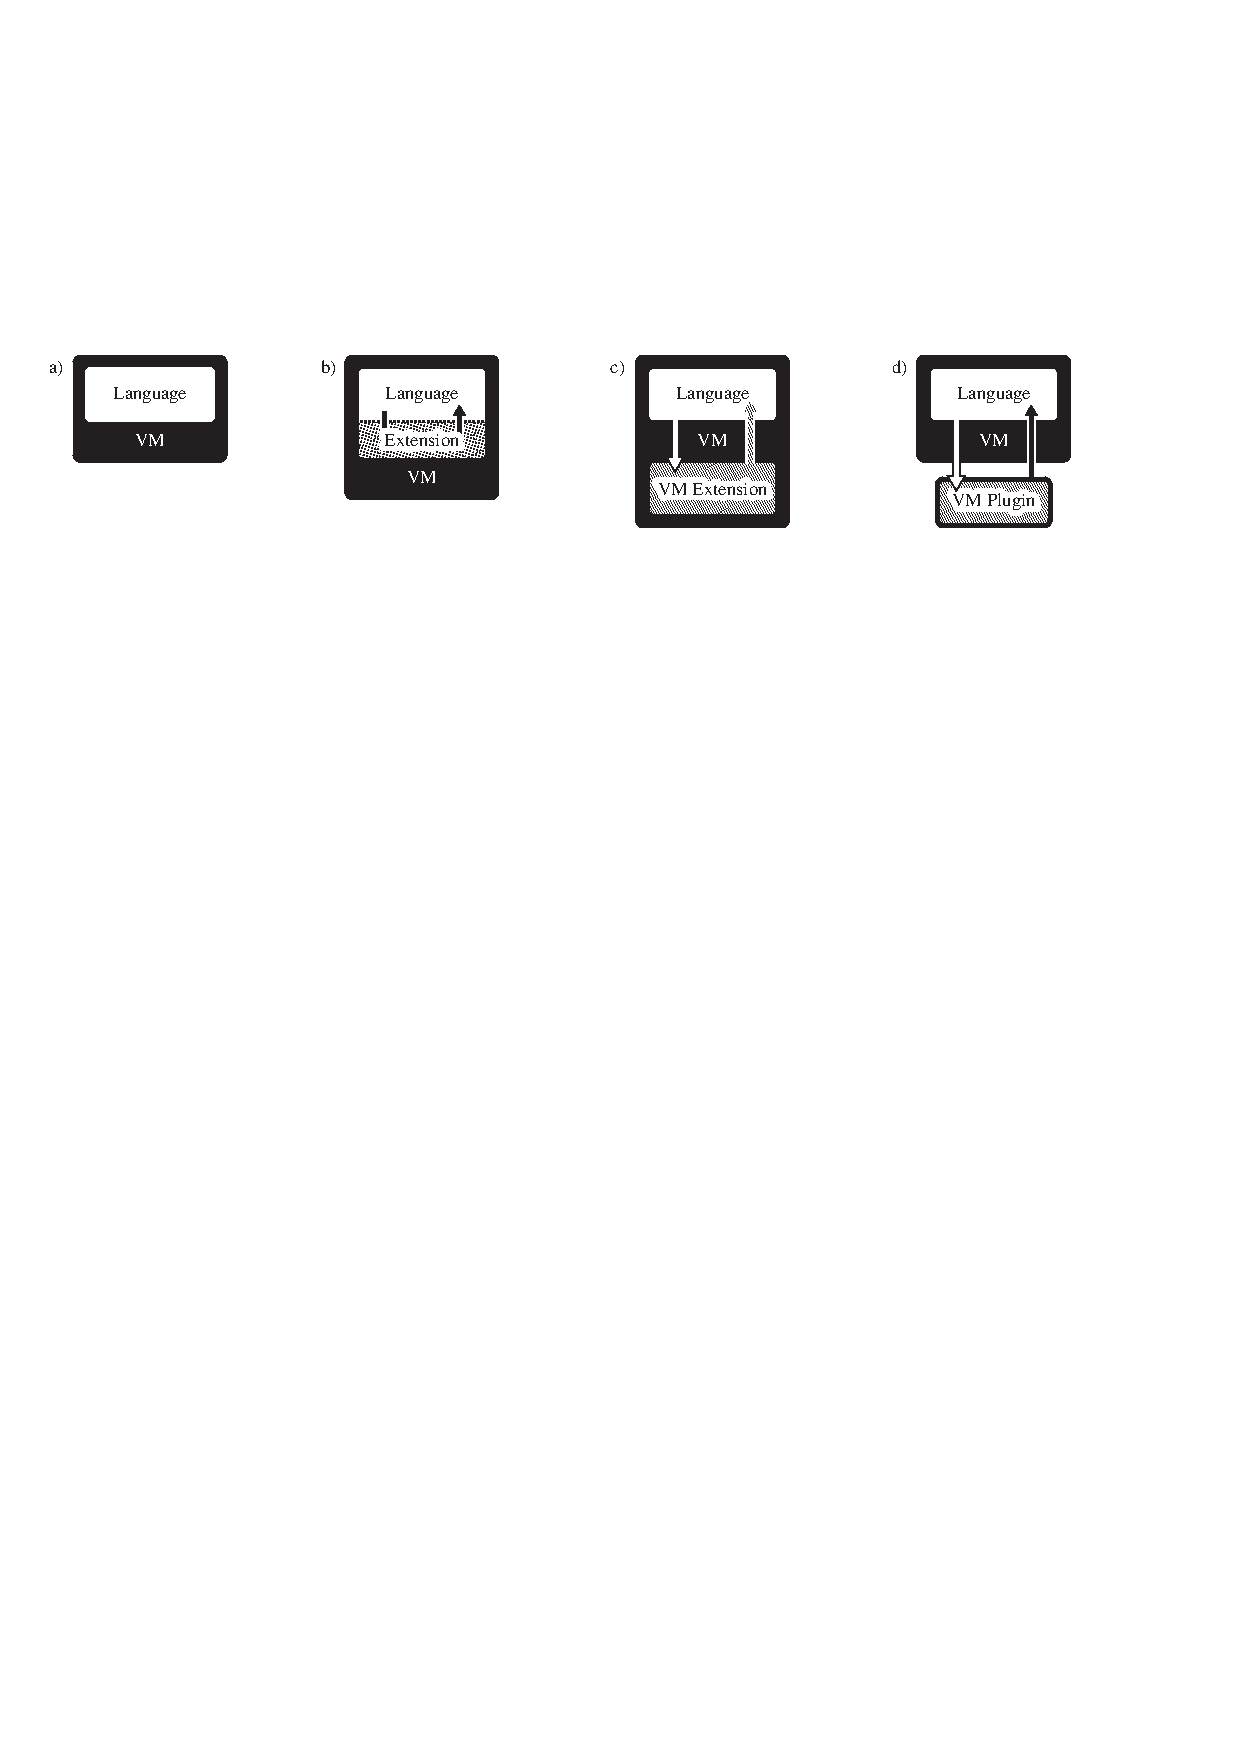
\includegraphics[width=\linewidth]{extensionComparison}
	\caption{Comparing different extension mechanisms: 
		a) language running on a standard VM, 
		b) language-side implementation of an extension
		c) language using features from a VM extension, 
		d) language using features from a separate VM plugin.}
	\figlabel{extensionComparison}
\end{figure}

%----------------------------------------------------------------------------
\subsubsection{Language-side Library.}

The most straight forward solution for extending a language is to write libraries within the language itself. 
This option provides the advantage that the aggregate behavior is accessible and evolvable for any language developer.
However, language-side libraries are constrained by the underlying managed language runtime.
The VM separates the language from the low-level internal details.
As a consequence language-side libraries are not feasible for all feature requirements.
For instance the previously mentioned example of instrumenting the language runtime is not possible as a standard language-side extension without a considerable performance loss.
So, even though we prefer extensions and optimizations at language-side, there are certain limitations of a managed language runtime that can not be circumvented.
If all language-side optimization opportunities have been exhausted it is exposing the need to resort to lower level approaches.
%\\

%\noindent\emph{Language-side libraries are constrained to the capabilities of the underlying VM and thus not general enough. Additionally not all performance bottlenecks can be addressed at language-side.}

%----------------------------------------------------------------------------
\subsubsection{Language-side Reflective Extensions.}

This is a subcase of the previous approach but in the context of reflective environments that expose particular characteristics.
For instance, Meta Object Protocols (MOP) \cite{Kicz91a} based on reflection \cite{Maes87a} are used to define certain control points in the system to change the language.
By composing meta objects it is possible to even modify the semantics of the language. 
Several languages such as Smalltalk, Python, and others provide reflective capabilities with different depths \cite{Ande98a,Flan08a,Van10a}.
However, most modern programming languages only have very limited support for intercession.
Hence the possibilities for dynamically changing language semantics or features are limited. 
Furthermore reflective capabilities are hard to implement efficiently.
Reflection imposes substantial performance penalties on most computations by postponing bindings \cite{Male96a}. 
Nevertheless, there are exceptions for a subset of reflective behavior which are implemented efficiently using a high-level MOP \cite{Vran12a}.
Though these approaches remain as a few exceptions.
In the typical low-level VM it is difficult to gain reflective access to language-side objects.
Similar to the previous case, our goal is to extend language features in a general way and it was shown that this is only partially possible by reflective extensions. 
%\\

%\noindent\emph{Reflective capabilities are not enough for general extensions. Even when suitable, they usually pose a significant performance overhead up to the point where they become unfeasible.}

%----------------------------------------------------------------------------
\subsubsection{VM Extensions.}
\seclabel{vm-extensions}

Another approach is to attach plugins to the VM.
Plugins are direct bindings to external libraries described at VM-side or libraries linked to the VM executable \cite[Ch.\ 5]{Blac09a}. 
They provide a performance boost in comparison to pure language-side solutions.
Using highly optimized native libraries it is straightforward to outperform code written at language-side.
However, plugins are commonly written in the same language as the VM, at a low abstraction level.
Few exceptions are self-hosted languages \cite{Unga05a,Wimm13a,Rigo06a}.
To support a fluent development process, VMs should come with an infrastructure for building extensions at same abstraction level than the language.
Instead they tend to be very complex and to have sluggish building processes. For example, only a few VMs have high-level debugging facilities \cite{Inga97a,Unga05a,Wimm13a}.
Also from a VM maintenance point of view, extensions have to be avoided if possible and should only be used for critical performance issues that can not be properly addressed at language-side.
An example of how the complexity of the VM can affect development efforts is the core of the Self VM \cite{Unga07a}.
After reduced development resources parts of the complex but efficient compiler infrastructure had to be abandoned in favor of a more maintainable code-base.

\todo{properly integrate}
High-level low-level programming \cite{Fram09a} encourage to use high-level languages for system programming.
Frampton et al. present a low-level framework packaged as \textsc{org.vmmagic}, which is used as system interface for Jikes, an experimental Java VM.
Additionally their framework is successfully used in MMTK \cite{Blac04a} which is used independently in several other projects.
The \textsc{org.vmmagic} package is much more elaborate than \B but it is tailored towards Java with static types.
Methods have to be annotated to use low-level functionality.
Additionally the strong separation between low-level code and language-side application does not allow for reflective extensions of the language runtime.
Finally, they do not support the execution nor generation of custom assembly code in the fly.

Other related approaches are VM generation frameworks in general.
They try to abstract away the complexity of the VM and use high-level languages as compiler infrastructure.
A very successful research project is Jikes Research VM \cite{Jikes}.
It uses Java to metacircularly define a Java environment which then generates the final VM.
A similar framework is PyPy \cite{Rigo06a} a VM framework including an efficient JIT. 
PyPy uses a restricted subset of the Python language named RPython which is then translated to various low-level backends such as C or LLVM code.
There exist several different high-level language VM implementations on top of PyPy such as \ST \cite{Bolz08a} or Prolog.
However, its main focus lies on an efficient JIT generator mainly for a Python interpreter, and not on a direct, language-side assembler interface.


%----------------------------------------------------------------------------
\subsubsection{Hybrid Extensions.}
The last approach is to reuse an existing library usually implemented in a foreign language.
The languages interact through a well-defined Foreign Function Interface (FFI).
FFI-based extensions are an hybrid approach between pure language-side extensions and VM-side ones.
Interaction with native libraries is supported by a dedicated VM functionality for calling external functions.
This allows for a smooth interaction of external code and language-side code.
FFI based extensions share the benefits of a maintainable and efficient language-side library with modest implementation efforts.
However, FFI is only a bridge or interface for allowing the interaction of different languages. 
It is not possible to directly synthesize new native features from language-side.
For this purpose we have to interact with a custom-made native library.
From an extension point of view this is close to the VM extensions discussed previously.

Additionally to the interface limitations, there exists a performance overhead in FFI for making the interaction between different languages possible. 
This is due to marshalling arguments and types between both languages \cite{Fish00a,Repp06b}.


Other high-level languages such as Lua leverage FFI performance by using a close interaction with the JIT.
LuaJIT \cite{luaffi} for instance is an efficient Lua implementation that inlines FFI calls directly into the JIT compiled code.
Similar to \B this allows to minimize the constant overhead by generating custom-made native code.
LuaJIT is mainly written in C which has clearly different semantics than Lua itself.
Compared to \ugh{our} approach the efficient VM implementation suffers from the shortcomings described in Section \secref{vm-extensions}. 

Kell and Irwin \cite{Kell11a} take a different look at interacting with external libraries.
They advocate a Python VM that allows for dynamically shared objects with external libraries.
It uses the low-level DWARF debugging information present in the external libraries to gather enough metadata to automatically generate FFIs.
However, they do not focus on the reflective interaction with low-level code and the resulting benefits. 

QUICKTALK \cite{Ball86a} follows a similar approach as Waterfall.
However, Ballard et al. focus mostly on the development of a complex compiler for a new \ST dialect.
Using type annotations QUICKTALK allows for statically typing methods.
By inlining methods and eliminating the bytecode dispatch overhead by generating native code QUICKTALK outperforms interpreted bytecode methods.
Compared to Waterfall QUICKTALK does not allow to leave the language-side environment and interact closely with the VM.
Hence it is not possible to use QUICKTALK to modify essential primitives.

A notable exception to the metacircular VMs mentioned earlier is the Self implementation Klein \cite{Unga05a}.
Unlike typical other metacircular approaches it does not strictly separate compile-time and runtime.
The reified VM concepts are available at runtime, which is a result from implementing the typical VM pieces at language-side.
Compared to our approach, Klein's bridging efforts are much more complete.
However, Klein is built on a completely new VM infrastructure, whereas \B requires only few changes to achieve its functionality.


% ===========================================================================
\section{Problems of Benzo}
\seclabel{problems}
% ===========================================================================
\todo{most problems are related to the missing debugging facilities}


% -----------------------------------------------------------------------------
\subsection{Robustness}
% -----------------------------------------------------------------------------
\todo{show a problematic piece of code}
\todo{sketch an outline for a safe benzo test by forking the main process}
\todo{image + code example}
\todo{possible emulation of the code to highlight very common bugs?}


% -----------------------------------------------------------------------------
\subsection{Low-level Debugging}
% -----------------------------------------------------------------------------
\todo{sketch a possible debugger with ptrace and Co based on the previously forked process}
\todo{outlook to the FFI section (reified structures)}
\todo{hard to debug when only looking at the memory}
\todo{- need full stack view}
\todo{- need register view}
\todo{- need possible view on references to ST objects}

% -----------------------------------------------------------------------------
\subsection{Platform Independence}
% -----------------------------------------------------------------------------
\todo{missing abstraction on the assembler level}
\todo{- outlook to the VirtualCPU}
\todo{- image: mini architecture picture}


% ===========================================================================
\section{Conclusion and Summary}
\seclabel{conclusion}
% ===========================================================================
\todo{Extend to full summary}
We presented \B, an integral approach for reflective high-level low-level programming.
Using \B we efficiently implemented at language-side three distinct language feature extensions that typically reside at VM-level.
\B promotes a smooth and powerful interaction with the low-level world by dynamically generating native code from language-side.
This enables to exploit the underlying platform capabilities only when strongly needed without leaving the development platform and through a high-level programming interface. 
As a result, \B advocates the use of development tools and abstraction level of the high-level language for as much as possible or desired.

By combining high-level reflection capabilities with efficient low-level code we manage to do dynamic primitive instrumentation and reuse the code for primitive operations which is duplicated on the standard JIT approach.
We also show that since \B caches native code transparently at language-side our JIT compiler poses only a one-time overhead when generating native code. 
Finally, we also show how our mature FFI implementation outperforms an existing C-FFI implementation by a factor of 1.5 even though we control every aspect from language-side.


As a final conclusion, \B shows that promoting clear interfaces for controlling low-level code completely from language-side produces efficient solutions for system programming requirements without resorting to pure low-level solutions.
We showed that fostering the abstraction provided by high-level languages and resorting to the system programming capabilities of low-level languages only when completely needed is not only possible but profitable.
Furthermore we manage to considerably reduce complexity and code duplication which results in better maintainability.



% =============================================================================
\ifx\wholebook\relax\else
    \end{document}
\fi
\documentclass[a4paper,12pt,twoside]{../includes/ThesisStyle}
\usepackage[utf8]{inputenc}
\usepackage[T1]{fontenc}

\usepackage[left=1.5in,right=1.3in,top=1.1in,bottom=1.1in,includefoot,includehead,headheight=13.6pt]{geometry}\renewcommand{\baselinestretch}{1.05}


% =============================================================================
%\usepackage[sectionbib]{chapterbib}	% Cross-reference package (Natural BiB)
%\usepackage{bibunits}
%\usepackage{natbib}					% Put References at the end of each chapter
\usepackage{algorithm}
\usepackage{alltt}
\usepackage{amsfonts}
\usepackage{amsmath}
\usepackage{amssymb}
\usepackage{cite}
\usepackage{color}
\usepackage{enumerate}
\usepackage{booktabs} % used for \midrule
\usepackage{fancyhdr}					% Fancy Header and Footer
\usepackage{graphicx}
\usepackage{ifthen}
\usepackage{latexsym}
\usepackage{multirow}
\usepackage{rotating}					% Sideways of figures & tables
\usepackage{stmaryrd}
\usepackage{subfigure}
\usepackage{url}         
\usepackage{xspace}
\usepackage[normalem]{ulem} % for \sout
\usepackage{xcolor}
\usepackage{tablefootnote}
\usepackage{pifont}

% =============================================================================

% Table of contents for each chapter
\usepackage[nottoc, notlof, notlot]{tocbibind}
\usepackage{minitoc}
\setcounter{minitocdepth}{1}
\mtcindent=15pt

\setcounter{secnumdepth}{3}
\setcounter{tocdepth}{2}
  
% =============================================================================
% Fancy Header Style Options

\pagestyle{fancy}                       % Sets fancy header and footer
\fancyfoot{}                            % Delete current footer settings

%\renewcommand{\chaptermark}[1]{         % Lower Case Chapter marker style
%  \markboth{\chaptername\ \thechapter.\ #1}}{}} %

%\renewcommand{\sectionmark}[1]{         % Lower case Section marker style
%  \markright{\thesection.\ #1}}         %

\fancyhead[LE,RO]{\bfseries\thepage}    % Page number (boldface) in left on even
% pages and right on odd pages
\fancyhead[RE]{\bfseries\nouppercase{\leftmark}}      % Chapter in the right on even pages
\fancyhead[LO]{\bfseries\nouppercase{\rightmark}}     % Section in the left on odd pages

\let\headruleORIG\headrule
\renewcommand{\headrule}{\color{black} \headruleORIG}
\renewcommand{\headrulewidth}{1.0pt}
\usepackage{colortbl}
\arrayrulecolor{black}

\fancypagestyle{plain}{
  \fancyhead{}
  \fancyfoot{}
  \renewcommand{\headrulewidth}{0pt}
}


% =============================================================================
% Clear Header Style on the Last Empty Odd pages
\makeatletter

\def\cleardoublepage{\clearpage\if@twoside \ifodd\c@page\else%
  \hbox{}%
  \thispagestyle{empty}%              % Empty header styles
  \newpage%
  \if@twocolumn\hbox{}\newpage\fi\fi\fi}

\makeatother

\newenvironment{maxime}[1]
{
\vspace*{0cm}
\hfill
\begin{minipage}{0.5\textwidth}%
%\rule[0.5ex]{\textwidth}{0.1mm}\\%
\hrulefill $\:$ {\bf #1}\\
%\vspace*{-0.25cm}
\it 
}%
{%

\hrulefill
\vspace*{0.5cm}%
\end{minipage}
}

\let\minitocORIG\minitoc
\renewcommand{\minitoc}{\minitocORIG \vspace{1.5em}}


\renewcommand{\epsilon}{\varepsilon}

% centered page environment
\newenvironment{vcenterpage}
	{\newpage\vspace*{\fill}\thispagestyle{empty}\renewcommand{\headrulewidth}{0pt}}
	{\vspace*{\fill}}
	

%=============================================================================

\usepackage{needspace}
\newcommand{\needlines}[1]{\Needspace{#1\baselineskip}}

\usepackage{xcolor}
\definecolor{source}{gray}{0.95}
% source code formatting
\usepackage{listings}
    % global settings for source code listing package
\lstset{
    basicstyle=\ttfamily\small,
    showspaces=false,
    showstringspaces=false,
    captionpos=b, 
    columns=fullflexible}

\lstdefinelanguage{ST}{
    keywordsprefix=\#,
    morekeywords=[0]{true,false,nil},
    morekeywords=[1]{self,super,thisContext},
    morekeywords=[2]{ifTrue:,ifFalse:,whileTrue:,whileFalse:,and:,or:,xor:,not:,by:,timesRepeat:},
    sensitive=true,
    morecomment=[s]{"}{"},
    morestring=[d]',
    escapechar={!},
    alsoletter={., :, -, =, +, <},
    moredelim=**[is][\itshape]{/+}{+/},
    literate=
        {^}{{$\uparrow$}}1
        {:=}{{$\leftarrow$}}1
        {~}{{$\sim$}}1
        {-}{{\sf -\hspace{-0.13em}-}}1  % the goal is to make - the same width as +
        {+}{\raisebox{0.08ex}{+}}1		% and to raise + off the baseline to match V
        , % Don't forget the comma at the end!
    style=STStyle
}
\lstdefinestyle{STStyle}{
    tabsize=4,
    %frame=leftline,
    % frame=bl,
    %framerule=2pt,
    %rulecolor=\color{gray},
    % backgroundcolor=\color{white},
    %backgroundcolor=\usebeamercolor[bg]{listing},
    basicstyle=\ttfamily\small,
    keywordstyle=\bf\ttfamily,
    % stringstyle=\color{orange},
    stringstyle=\mdseries\slshape,
    commentstyle=\it\rmfamily\color{darkgray}, 
    commentstyle=\mdseries\slshape\color{gray},
    %commentstyle=\mdseries\slshape,
    emphstyle=\bf\ttfamily,
    escapeinside={!}{!},
	%backgroundcolor=\color{source},
    %emphstyle={[2]\color{red}},
    %emphstyle={[3]\color{blue}\bf},
    %emphstyle={[4]\color{blue}},
    keepspaces=true
} 

%\lstnewenvironment{javacode}  [1][]{\lstset{language=java,#1}\needlines{#2}}{} 
%\lstnewenvironment{pythoncode}[2][]{\lstset{language=python,#1}\needlines{#2}}{}
\lstnewenvironment{stcode}    [2][]{\lstset{language=ST,#1}\needlines{#2}}{}
\lstnewenvironment{ccode}     [2][]
    {\lstset{language=C,numbers=left,escapechar=\$,numberstyle=\tiny,#1}\needlines{#2}}{}

% ON: I tried to pass the line number options in as arg #1 but it does not work for me
% I also could net get the line numbers to consistently increase
\lstnewenvironment{numstcode} [2][]
    {\lstset{language=ST,numbers=left,numberstyle=\tiny,numbersep=2pt,#1}\needlines{#2}}{}
\lstnewenvironment{numstcodecont} [2][]
    {\lstset{language=ST,numbers=left,numberstyle=\tiny,numbersep=2pt,firstnumber=last#1}\needlines{#2}}{}

\newcommand{\lst}[1]{{\tt #1}}

% In-line code (literal)

% In-line code (latex enabled)
% Use this only in special situations where \ct does not work
% (within Section headings ...):
\newcommand{\lct}[1]{{\textsf{\textup{#1}}}}
% Code environments
\lstnewenvironment{code}{%
	\lstset{%
		% frame=lines,
		frame=single,
		framerule=0pt,
		mathescape=false
	}
}{}

%\renewcommand{\lstlistingname}{Code Example}

% =============================================================================
\newboolean{showcomments}
\setboolean{showcomments}{true}

\ifthenelse{\boolean{showcomments}} {
	\newcommand{\ugh}[1] {\textcolor{red}{\uwave{#1}}}	% please rephrase
	\newcommand{\ins}[1] {\textcolor{blue}{\uline{#1}}}	% please insert
	\newcommand{\del}[1] {\textcolor{red}{\sout{#1}}}	% please delete
	\newcommand{\chg}[2] {								% please change
		\textcolor{red}{\sout{#1}}{\ra}
		\textcolor{blue}{\uline{#2}}}
	\newcommand{\nbc}[3]{								% comment
		{\colorbox{#3}{\bfseries\sffamily\scriptsize\textcolor{white}{#1}}}
		{\textcolor{#3}{\sf\small$\blacktriangleright$\textit{#2}$\blacktriangleleft$}}}

}{
	\newcommand{\ugh}[1]{#1}							% please rephrase
	\newcommand{\ins}[1]{#1}							% please insert
	\newcommand{\del}[1]{}								% please delete
	\newcommand{\chg}[2]{#2}							% please change
	\newcommand{\nbc}[3]{}								% comment
}

% =============================================================================
\usepackage[pagebackref,hyperindex=true]{hyperref}


% Links in pdf
\usepackage{color}
\definecolor{linkcol}{rgb}{0.0, 0.0, 0.0} 
\definecolor{citecol}{rgb}{0.0, 0.0, 0.0} 

% Change this to change the informations included in the pdf file
% See hyperref documentation for information on those parameters
\hypersetup {
	bookmarksopen=true,
	pdftitle="Design and Use of Anatomical Atlases for Radiotherapy",
	pdfauthor="Olivier COMMOWICK", 
	pdfsubject="Creation of atlases and atlas based segmentation", %subject of the document
	%pdftoolbar=false, % toolbar hidden
	pdfmenubar=true, %menubar shown
	pdfhighlight=/O, %effect of clicking on a link
	colorlinks=true,
	pdfpagemode=UseNone,
	pdfpagelayout=SinglePage,
	pdffitwindow=true,
	linkcolor=linkcol,
	citecolor=citecol,
	urlcolor=linkcol
}

% =============================================================================
\newcommand{\figlabel}[1] {\label{fig:#1}}
\newcommand{\chaplabel}[1]{\label{chap:#1}}
\newcommand{\seclabel}[1] {\label{sec:#1}}
\newcommand{\tablabel}[1] {\label{tab:#1}}
\newcommand{\lstlabel}[1] {\label{lst:#1}}

\newcommand{\figref}[1] {Figure~\ref{fig:#1}}
\newcommand{\chapref}[1]{Chapter~\ref{sec:#1}}
\newcommand{\secref}[1] {Section~\ref{sec:#1}}
\newcommand{\tabref}[1] {Table~\ref{tab:#1}}
\newcommand{\lstref}[1] {Listing~\ref{tab:#1}}

\newcommand{\commented}[1]{}

\newcommand{\bs}    {\symbol{'134}} % backslash
\newcommand{\us}    {\symbol{'137}} % underscore
\newcommand{\ttt}[1]{\texttt{#1}}
\newcommand{\ie}    {\emph{i.e.},\xspace}
\newcommand{\eg}    {\emph{e.g.},\xspace}
\newcommand{\etal}  {\emph{et al.}\xspace}
\newcommand{\ns}    {\!\!\!\!} %big negative space
\newcommand{\cnull} {\textbackslash0\xspace}


\newcommand\fix[1]{\nb{FIX}{#1}}
\newcommand\todo[1]{\nb{TO DO}{#1}}
\newcommand\cb[1]{\nbc{CB}{#1}{purple}}
\newcommand\sd[1]{\nbc{SD}{#1}{orange}}
\newcommand\is[1]{\nbc{IS}{#1}{gray}}
\newcommand\gc[1]{\nbc{GC}{#1}{olive}}
\newcommand\ct[1]{\nbc{CT}{#1}{teal}}
\newcommand\md[1]{\nbc{MD}{#1}{blue}}
\newcommand\dc[1]{\nbc{DC}{#1}{green}}

% =============================================================================
\newcommand{\NBFFI}  {Native\-Boost-FFI\xspace}
\newcommand{\NB}  {Native\-Boost\xspace}
\newcommand{\B}   {Benzo\xspace}
\newcommand{\ST}  {Small\-talk\xspace}
\newcommand{\PH}  {Pharo\xspace}
\graphicspath{{.}{../figures/}}

\begin{document}
% ==========================================================================
\chapter{Validation: \FFI}
\chaplabel{ffi}
\minitoc
% ===========================================================================
\introduction
% ===========================================================================
\todo{Intro referring to the benzo chapter}

% ===========================================================================
\newpage
\section{Background}
\seclabel{ffi-background}
% ===========================================================================

\begin{figure*}[ht]
	\centering
	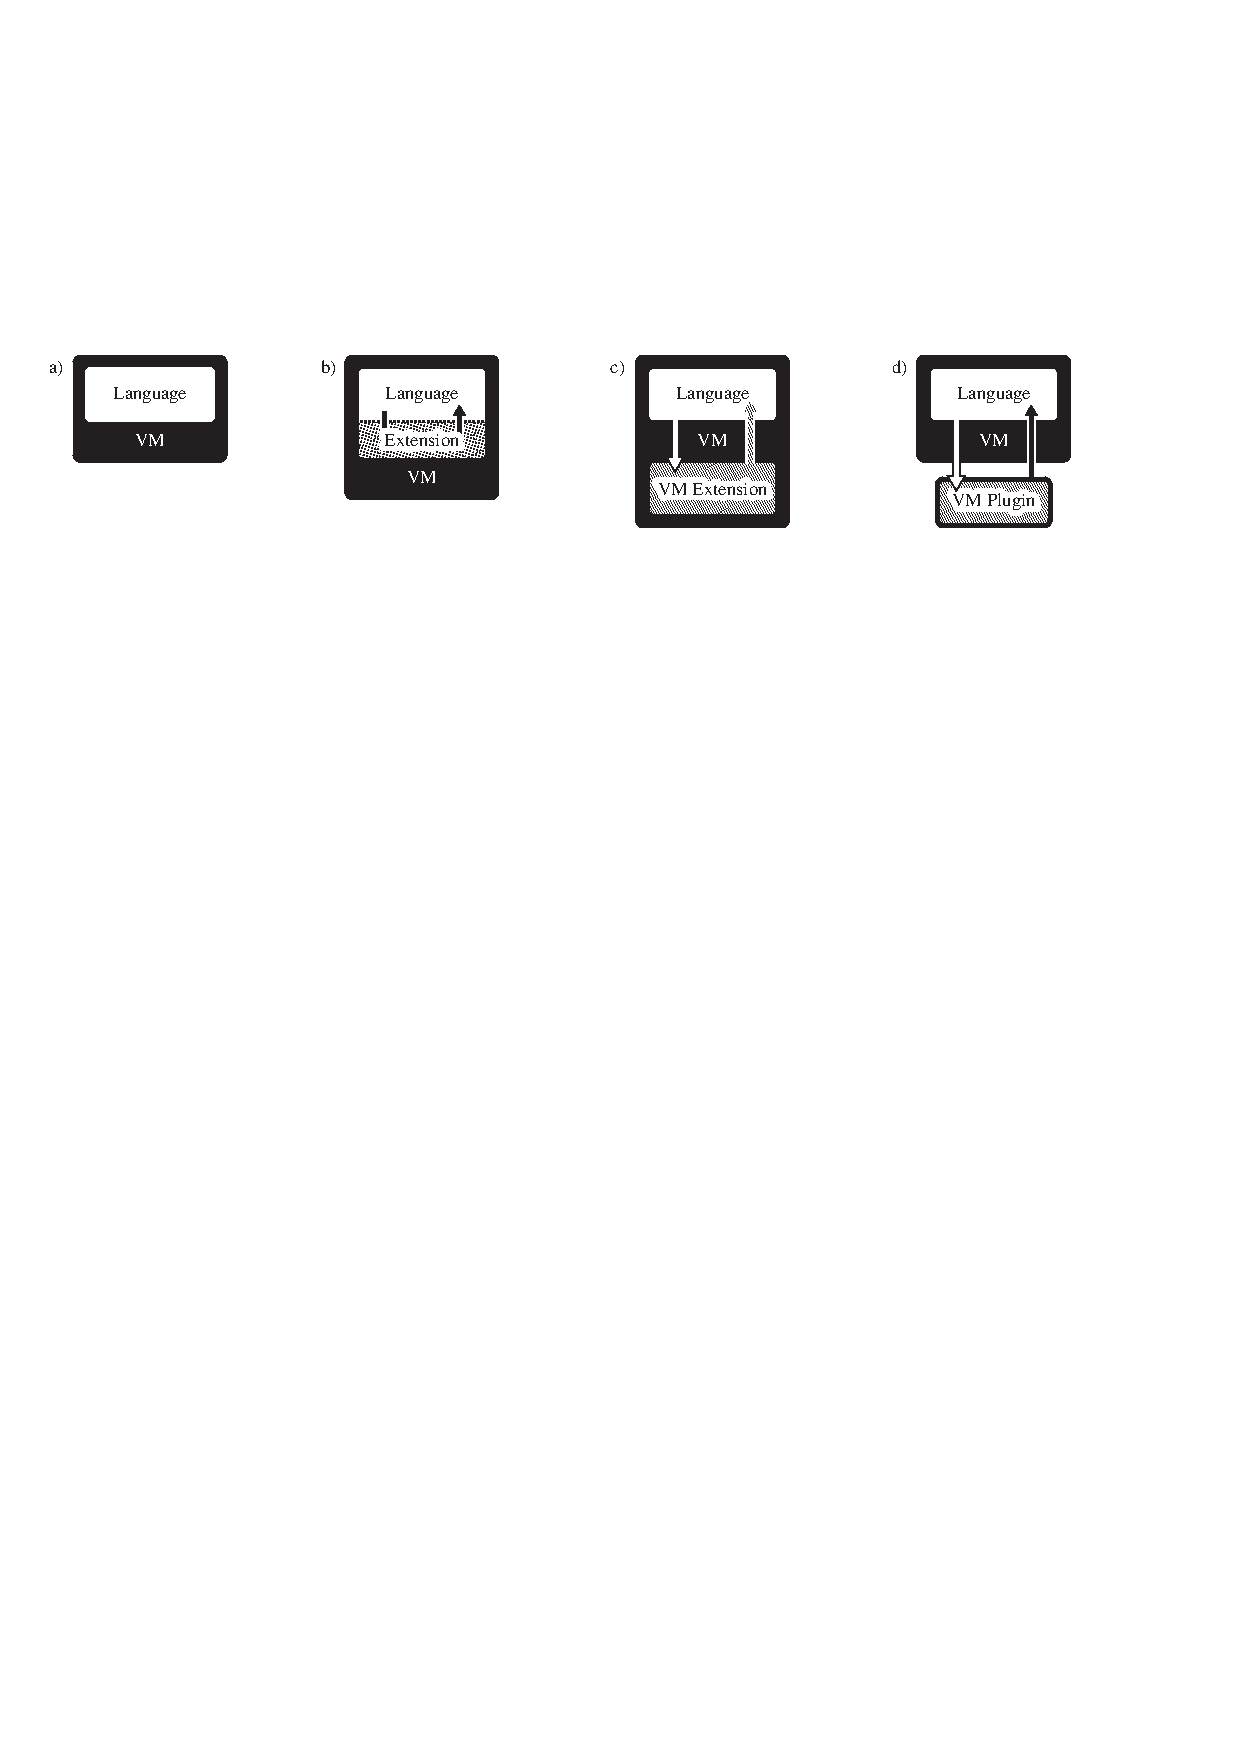
\includegraphics[width=\textwidth]{extensionComparison}
	\caption{\todo{clearly duplicated}Comparing different extension mechanisms: 
		a) library implemented completely at language-side running on a standard \VM,
		b) language using features from a \VM extension,
		c) language using features from a \VM plugin,
		d) language-side implementation of an extension.}
	\figlabel{ffi-extensionComparison}
\end{figure*}

Currently, more and more code is produced and available through reusable libraries such as OpenGL\footnote{\url{http://www.opengl.org/}} or Cairo\footnote{\url{http://cairographics.org/}}.
While working on your own projects using dynamic languages, it is crucial to be able to use such existing libraries with little effort.
Multiple solutions exist to achieve access to an external library from dynamic languages that are executed on the top of a virtual machine (\VM) such as \PH\footnote{\url{http://pharo.org/}}, \Lua\footnote{\url{http://lua.org/}} or \Python\footnote{\url{http://python.org/}}.
\figref{ffi-extensionComparison} depicts four possibilities of dealing with new or external libraries in a high-level language.

\paragraph{Language-side Library.}
One solution is to re-implement a library completely at language-side (cf. \figref{ffi-extensionComparison}.a).
Even though this is the most flexible solution, this is often not an option, neither from the technical point of view (performance penalty), nor from the economic point of view (development time and costs).

\paragraph{\VM Extension.}
The second one (\figref{ffi-extensionComparison}.b) is to do a \emph{\VM extension} providing new primitives that the high-level language uses to access the native external library.
This solution is generally efficient since the external library may be statically compiled within the \VM.
However a tight integration into the \VM also means more dependencies and a different development environment than the final product at language-side.

\paragraph{\VM Plugin.}
The third solution (\figref{ffi-extensionComparison}.c) is similar to the previous one but the extension is factored out of the \VM as a \emph{plugin}.
This solution implies again a lot of low-level development at \VM-level that must be done for each external library we want to use.
Additionally we have to adapt the plugin for all platforms on which the \VM is supposed to run on.

\paragraph{\FFI.}
A higher-level solution is to define \emph{Foreign Function Interfaces} (\FFIs) (cf. \figref{ffi-extensionComparison}.d).
The main advantage of this approach is that once a \VM is \FFI-enabled, only a language extension (no \VM-level code) is needed to provide access to new native libraries.
From the portability point of view, only the generic \FFI \VM-plugin has to be implemented on all platforms.

% Challenges & Goals
Implementing an \FFI library is a challenging task because of its antagonist goals:
\begin{itemize}
    \item it must be flexible enough to easily bind to external libraries and also express complex foreign calls regarding the memory management or the type conversions (marshalling);
    \item it must be well integrated with the language (objects, reflection, garbage collector);
    \item it must be efficient.
\end{itemize}
%
Existing \FFI libraries of dynamic languages all have different designs and implementations because of the trade-offs they made regarding these goals and challenges.
Typical choices are resorting purely to the \VM-level and thus sacrificing flexibility.
The inverse of this approach exists as well: \FFIs can be implemented almost completely at language-side but at a significant performance loss.
Both these pitfalls are presented in more detail in \secref{ffi-evaluation}.


% list shortcomings of typical implementations (C-\FFI vs ALIEN)
% - too low-level (C-\FFI) fast in simple examples, complex calls not possible
% - too high-level (ALIEN) slow in simple examples, quite slow in complex ones
% - missing specific code generation
% - missing \JIT interaction for speed (like LuaJIT, org.vmmagic)

% \Alien and C-\FFI run in the same \PH image as \NB allowing a much closer comparison.
% \Alien \FFI is implemented almost completely at language-side, much like \NB. However, as the following benchmarks will stress, it also suffers from performance loss.
% On the other end there is C-\FFI which is faster than \Alien but by far not as flexible. For instance only primitive types are handled directly.


This paper presents \NBFFI\footnote{\url{http://code.google.com/p/nativeboost}} an \FFI library at language-side for \PH that supports callouts and callbacks, which we present in \secref{ffi-nutshell}.
There are at least two other existing \FFI libraries in \PH worth mentioning: C-\FFI and \Alien.
Nevertheless, they both present shortcomings.
C-\FFI is fast because it is mostly implemented at \VM-level, however it is limited when it comes to do complex calls that involve non-primitive types or when we want to define new data types.
On the opposite, \Alien \FFI is flexible enough to define any kind of data conversion or new types directly at language-side but it is slower than C-\FFI because it is mostly implemented at language-side.
In essence, \NBFFI combines the flexibility and extensibility of \Alien that uses language-side definition for marshalling and the speed of C-\FFI which is implemented at \VM-level.
The main contributions of \NBFFI are:

\begin{description}
	\item[Extensibility.] \NBFFI relies on as few \VM primitives as possible (5 primitives), essentially to call native code. 
	Therefore, most of the implementation resides at language-side, even low-level mechanisms.
	That makes \NBFFI easily extensible because its implementation can be changed at any time, without needing to update the runtime (\VM).
	It also presents a noticeable philosophical shift, how we want to extend our language in future.
	A traditional approach is to implement most low-level features at \VM-side and provide interfaces to the language-side.
	But that comes at cost of less flexibility and longer development and release cycles.
	On the opposite, we argue that extending language features, even low-level ones, should be done at language-side instead.
	This results in higher flexibility and without incurring high runtime costs which usually happen when using high-level languages such as \ST.
	\item[Language-side extension.] Accessing a new external library using \NBFFI involves a reduced amount of work since it is only a matter of writing a language-side extension.
	\item[Performance.] Despite the fact it is implemented mostly at language-side, \NBFFI achieves superior performance compared to other \FFI implementations running \PH.
    This is essentially because it uses automatic and transparent native code generation at language-side for marshalling.
\end{description}

%In the following section we present the language-side code that one should write to achieve to interact with external libraries with \NBFFI.
%We then compare performance of \NBFFI with three other \FFI implementations in \secref{ffi-evaluation}.
%The following \secref{ffi-internals} gives more insights on the \NB.
%After the related work presented in \secref{ffi-relatedWork} and we conclude this paper in \secref{ffi-conclusion}.


% ===========================================================================
\section{\NBFFI: an Introduction}
\seclabel{ffi-nutshell}
% ===========================================================================

This section gives an overview of the code that should be written at language-side
to enable interactions with external libraries.


% ---------------------------------------------------------------------------
\subsection{Simple Callout}
% ---------------------------------------------------------------------------

\lstref{ffi-clock} shows the code of a regular \ST method named \ttt{ticksSinceStart} that defines a callout to the \ttt{clock} function of the \ttt{libc}.
\NB imposes no constraint on the class in which such a binding should be defined.
However, this method must be annotated with a specific pragma (such as \ttt{<primitive:module:>}) which specifies that a native call should be performed using the \NB plugin.

\begin{stcode}[
	label={lst:ffi-clock},
	caption={\NBFFI example of callout declaration to the \ttt{clock} function of the \ttt{libc}}]{0}
ticksSinceStart
	<primitive: #primitiveNativeCall
	 module: #NativeBoostPlugin>
	^ self
		nbCall: #(uint clock ())
		module: NativeBoost CLibrary
\end{stcode}

The external function call is then described using the \ttt{nbCall:module:} message.
The first parameter (\ttt{\#nbCall:}) is an array that describes the signature of C function to callout.
Basically, this array contains the description of a C function prototype, which is very close to normal C syntax.
The return type is first described (\ttt{uint} in this example\footnote{The return type of the \ttt{clock} function is \ttt{clock\_t}, but we deliberately used \ttt{uint} in this first example for the sake of simplicity even if it is possible to define a constant type in \NB.}), then the name of the function (\ttt{clock}) and finally the list of parameters (an empty array in this example since \ttt{clock} does not have any).
The second argument, \ttt{\#module:} is the module name, its full path or its handle if already loaded, where to look up the given function.
This example uses a convenience method of \NB named \ttt{CLibrary} to obtain a handle to the standard C library.

% ---------------------------------------------------------------------------
\subsection{Callout with Parameters}
% ---------------------------------------------------------------------------

% - explain argument detection (match var names)
\figref{ffi-nativeBoostSyntax} presents the general syntax of \NBFFI through an example of a callout to the \ttt{abs} function of the \ttt{libc}.
The \ttt{abs:} method has one argument named \ttt{anInteger} (cf. \ding{182}).
This method uses the pragma \ttt{<primitive:module:error:>} which indicates that the \ttt{\#primitiveNativeCall} of the \ttt{\#NativeBoostPlugin} should be called when this method is executed (cf. \ding{183}).
An \ttt{errorCode} is returned by this primitive if it fails and the regular \ST code below is executed (cf. \ding{184}).
The main difference with the previous example is that the \ttt{abs} function takes one integer parameter.
In this example, the array \ttt{\#(uint abs(int anInteger))} passed as argument to \ttt{\#nbCall:} contains two important information (cf. \ding{185}).
First, the types annotations such as the return type (\ttt{uint} in both examples) and arguments type (\ttt{int} in this example).
These types annotations are then used by \NBFFI to automatically do the marshalling between C and \PH values as illustrated by the next example.
Second, the values to be passed when calling out.
In this example, \ttt{anInteger} refers to the argument of the \ttt{abs} method, meaning that the value of this variable should be passed to the \ttt{abs} C function.
Finally, this \ttt{abs} function is looked up in the \ttt{libc} whose an handle is passed in the \ttt{module:} parameter (cf. \ding{186}).
% A library can be designated either by its file path on disk or its memory address.
% \begin{stcode}[
% 	label={lst:abs},
% 	caption={Example of callout to the \ttt{abs} function}]{0}
% abs: anInteger
% 	<primitive: #primitiveNativeCall
% 	 module: #NativeBoostPlugin>
%
% 	^ self
% 		nbCall: #(uint abs(int anInteger))
% 		module: NativeBoost CLibrary
% \end{stcode}
%
% - explain syntax in picture (line plus arrows)
\begin{figure}[H]
	\centering
	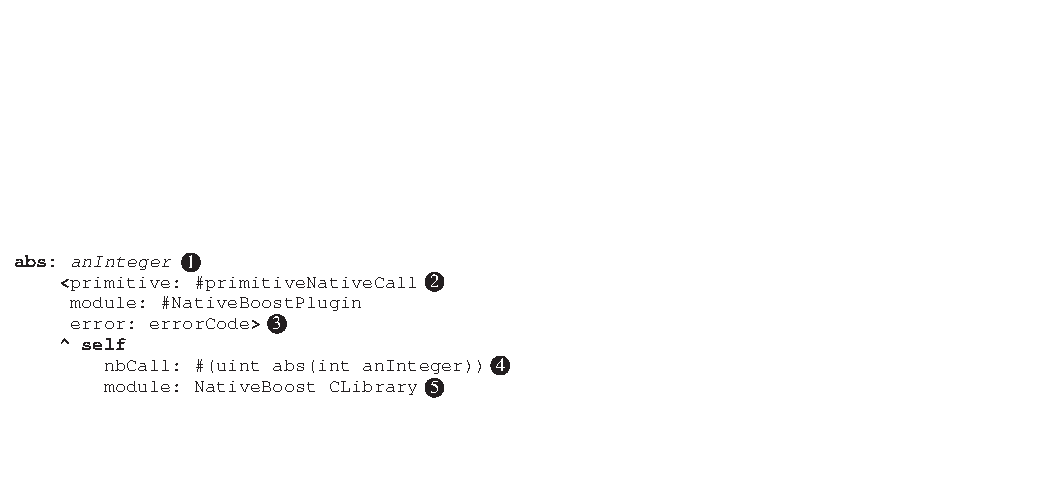
\includegraphics{nativeBoostSyntax}
	\caption[\NB Basic Method]{Example of the general \NBFFI callout syntax}
	\figlabel{ffi-nativeBoostSyntax}
\end{figure}

% ---------------------------------------------------------------------------
\subsection{Automatic Marshalling of Known Types}
% ---------------------------------------------------------------------------

\lstref{ffi-getenv} shows a callout declaration to the \ttt{getenv} function that takes one parameter.
%
\begin{stcode}[
	label={lst:ffi-getenv},
	caption={Example of callout to \ttt{getenv}}]{0}
getenv: name
	<primitive: #primitiveNativeCall
	 module: #NativeBoostPlugin>

	^ self
		nbCall: #(String getenv(String name)
		module: NativeBoost CLibrary
\end{stcode}
%
In this example, the \NB type specified for the parameter is \ttt{String} instead of \ttt{char*} as specified by the standard \ttt{libc} documentation.
This is on purpose because strings in C are sequences of characters (\ttt{char*}) but they must be terminated with the special character: \cnull.
Specifying \ttt{String} in the \ttt{\#nbCall:} array will make \NB to automatically do the arguments conversion from \ST strings to C strings (\cnull terminated \ttt{char*}).
It means that the string passed will be put in an external C \ttt{char} array and a \cnull character will be added to it at the end.
This array will be automatically released after the call returned.
This is an example of automatic memory management of \NB that can also be controlled if needed.
Obviously, the opposite conversion happens for the returned value and the method returns a \ST String.
This example shows that \NBFFI accepts literals, local and instance variable names in callout declarations and it uses their type annotation to achieve the appropriate data conversion.
\tabref{ffi-nbPrimitiveTypes} shows the default and automatic data conversions achieved by \NBFFI.

\begin{table}[hbt]
    \centering
    \begin{tabular}{rll}
        Primitive Type       & \ST Type \\\midrule
        \ttt{uint}   & \ttt{Integer} \\
        \ttt{int}    & \ttt{Integer} \\
        \ttt{String} & \ttt{ByteString} \\
        \ttt{bool}   & \ttt{Boolean} \\
        \ttt{float}  & \ttt{Float} \\
        \ttt{char}   & \ttt{Character} \\
        \ttt{oop}    & \ttt{Object}
    \end{tabular}
    \caption[\NB Primitive Types]{Default \NBFFI mappings between C/primitive types and high-level types.Note that \ttt{oop} is not a real primitive type as no marshalling is applied and the raw pointer is directly exposed to \PH.}
    \tablabel{ffi-nbPrimitiveTypes}
\end{table}
%
\lstref{ffi-setenv} shows another example to callout the \ttt{setenv} function.
The return value will be converted to a \ST \ttt{Boolean}.
The two first parameters are specified as \ttt{String} and will be automatically transformed in \ttt{char*} with an ending \cnull character.
The last parameter is \ttt{1}, a \ST literal value without any type specification and \NB translates it as an \ttt{int} by default.

\begin{stcode}[
	label={lst:ffi-setenv},
	caption={Example of callout to \ttt{setenv}}]{0}
setenv: name value: value
	<primitive: #primitiveNativeCall
	 module: #NativeBoostPlugin>

	^ self
		nbCall: #(Boolean setenv(String name,
								 String value,
								 1)
		module: NativeBoost CLibrary
\end{stcode}

Another interesting example of automatic marshalling is to define the \ttt{abs} method (cf. \figref{ffi-nativeBoostSyntax}) in the \ttt{SmallInteger} class and passing \ttt{self} as argument in the callout.
In such case, \NB automatically converts \ttt{self} (which is a \ttt{SmallInteger}) into an \ttt{int}.
This list of mapping is not exhaustive and \NB also supports the definition of new data types and new conversions into more complex C types such as structures (cf. \secref{ffi-internals}).



% memory alloc & structs
\begin{table}[t]
    \centering
    \begin{tabular}{lcccc}
                    &  Memory 	    & Address  & Marshalling         & Constraint  \\\midrule
C-managed struct 	&  C heap  	    & fixed    & passed by reference & must be freed \\
\PH-managed struct  & Object memory & variable & passed by reference & may move \\
& & & or passed by copy & costly\\
    \end{tabular}
    \caption{Wrapping structures possibilities in \NB}
    \tablabel{ffi-wrappingstruct}
\end{table}


% ---------------------------------------------------------------------------
\subsection{Supporting new types}
\seclabel{ffi-newtypes}
% ---------------------------------------------------------------------------

The strength of language-side \FFIs appears when it comes to do callouts with new data types involved.
\NBFFI supports different possibilities to interact with new types.

\paragraph{Declaring structures.}
For example, the Cairo library\footnote{\url{http://cairographics.org}} provides complex structures such as \ttt{cairo\_surface\_t} and functions to manipulate this data type. % which makes field access useless.
\lstref{ffi-AthensCairoSurface} shows how to write a regular \ST class to wrap a C structure.
\NB only requires a class-side method named \ttt{asNBExternalType:} that describes how to marshall this type back and forth from native code.
In this example, we use existing marshalling mechanism defined in \ttt{NBExternalObjectType} that just copies the structure's pointer and stores it in an instance variable named \ttt{handle}.

\begin{stcode}[
	label={lst:ffi-AthensCairoSurface},
	caption={Example of C structure wrapping in \NB}]{0}
AthensSurface subclass: #AthensCairoSurface
	instanceVariableNames: 'handle'.

AthensCairoSurface class>>asNBExternalType: gen
	"handle iv holds my address (cairo_surface_t)"
	^ NBExternalObjectType objectClass: self
\end{stcode}

\paragraph{Callout with structures.}
\lstref{ffi-calloutOpaqueStruct} shows a callout definition to the \ttt{cairo\_image\_surface\_create} function that returns a \ttt{cairo\_surface\_t*} data type.
In this code example, the return type is \ttt{AthensCairoSurface} directly (not a pointer).
When returning from this callout, \NB creates an instance of \ttt{AthensCairoSurface} and the marshalling mechanism  stores the returned address in the \ttt{handle} instance variable of this object.

\begin{stcode}[
	label={lst:ffi-calloutOpaqueStruct},
	caption={Example of returning a structure by reference}]{0}
primImage: aFormat width: aWidth height: aHeight
	<primitive: #primitiveNativeCall
	 module: #NativeBoostPlugin
     error: errorCode>

	^self nbCall: #(AthensCairoSurface
		cairo_image_surface_create (int aFormat,
									int aWidth,
									int aHeight) )
\end{stcode}

Conversely, passing an \ttt{AthensCairoSurface} object as a parameter in a callout makes its pointer stored in its \ttt{handle} iv (cf. \lstref{ffi-calloutOpaqueStructParameter}) to be passed.
Since the parameter type is \ttt{AthensCairoSurface} in the callout definition, \NB also ensures that the passed object is really an instance of this class.
If it is not, the callout fails before executing the external function because passing it an address on a non-expected data could lead to unpredicted behavior.

\begin{stcode}[
	label={lst:ffi-calloutOpaqueStructParameter},
	caption={Example of passing a structure by reference}]{0}
primCreate: cairoSurface
	<primitive: #primitiveNativeCall
	 module: #NativeBoostPlugin>

	^self nbCall: #(
        AthensCairoCanvas cairo_create (
                  AthensCairoSurface cairoSurface))
\end{stcode}


\paragraph{Accessing structure fields.}
In \NB, one can directly access the fields of a structure if needed, even if it is not a good practice from the data encapsulation point of view.
Nevertheless, it may be mandatory to interact with some native libraries that do not provide all the necessary functions to manipulate the structure.
\lstref{ffi-cairo_c_definition} shows an example of a C struct type definition for \ttt{cairo\_matrix\_t}.

\begin{ccode}[
	label={lst:ffi-cairo_c_definition},
	caption={Example external type to convert back and forth with the Cairo library}]{0}
typedef struct {
    double xx; double yx;
    double xy; double yy;
    double x0; double y0;
} cairo_matrix_t;
\end{ccode}

\noindent \lstref{ffi-AthensCairoMatrix} shows that the \ttt{NBExternalStructure} of \NBFFI can be subclassed to define new types such as \ttt{AthensCairoMatrix}.
The description of the fields (types and names) of this structure is provided by the \ttt{fieldsDesc} method on the class side.
Given this description, \NB lazily generates field accessors on the instance side using the field names.

\begin{stcode}[
	label={lst:ffi-AthensCairoMatrix},
	caption={Example of \NBFFI definition of an \ttt{ExternalStructure}}]{0}
NBExternalStructure
    variableByteSubclass: #AthensCairoMatrix.

AthensCairoMatrix class>>fieldsDesc
	^ #(  double sx; double shx;
		  double shy; double sy;
		  double x; double y;  )
\end{stcode}

\noindent \lstref{ffi-cairoCallouts} shows a callout definition to the
 \ttt{cairo\_matrix\_multiply} function passing \ttt{self} as argument with the type \ttt{AthensCairoMatrix*}.
\NB handles the marshalling of this object to a struct as defined in the \ttt{fieldsDesc}.
% The interesting point is that the called function \ttt{cairo\_matrix\_multiply} stores its result in the first argument i.e. the receiver object.

\begin{stcode}[
	label={lst:ffi-cairoCallouts},
	caption={Example of callouts using \ttt{cairo\_matrix\_t}}]{0}
AthensCairoMatrix>>primMultiplyBy: m
	<primitive: #primitiveNativeCall
	 module: #NativeBoostPlugin
     error: errorCode>

"C signature"
"void cairo_matrix_multiply (
                     cairo_matrix_t *result,
                     const cairo_matrix_t *a,
                     const cairo_matrix_t *b );"
	^self nbCall: #(void   cairo_matrix_multiply
		(AthensCairoMatrix * self,
		AthensCairoMatrix * m ,
		AthensCairoMatrix * self ) )
\end{stcode}


\paragraph{Memory management of structures.}
\tabref{ffi-wrappingstruct} shows a comparison between C-managed and \PH-managed structures.
The first ones are allocated in the C heap.
Their addresses are fixed and they are passed by reference during a callout.
But the programmer must free them by hand when they are not needed.
The second ones are allocated in the \PH object-memory.
Their addresses are variable since their enclosing object may be moved by the garbage collector.
They can either passed by copy which is costly or by reference.
Passing a reference may lead to problems is the C function stores the address and try to access it later on since the address may changed.


% ---------------------------------------------------------------------------
\subsection{Callbacks}
% ---------------------------------------------------------------------------

\NB supports callbacks from native code.
This means it is possible for a C-function to call back into the \PH runtime and activate code.
We will use the simple \ttt{qsort} C-function to illustrate this use-case.
\ttt{qsort} sorts a given array according to the results of a compare function.
Instead of using a C-function to compare the elements we will use a callback to invoke a \PH block which will compare the two arguments.
%
\begin{stcode}[
	label={lst:ffi-calloutWithCallback},
	caption={Example of callout passing a callback for \ttt{qsort}}]{0}
bytes := #[ 120 12 1 15 ].
callback := QSortCallback on: [ :a :b |
				(a byteAt: 0) - (b byteAt: 0) ].

self ffiQSort: bytes
	 length: bytes size
	 compareWith: callback
\end{stcode}
%
Code \lstref{ffi-calloutWithCallback} shows the primary \PH method for invoking \ttt{qsort} with a \ttt{QSortCallback} instance for the compare function.
In this example \ttt{qsort} will invoke run the \PH code inside the callback block to compare the elements in the \ttt{bytes} array.

To define a callback in \NB we have to create a specific subclasses for each callback with different argument types.
%
\begin{stcode}[
	label={lst:ffi-callbackDefinition},
	caption={Example of callback definition}]{0}

NBFFICallback
    subclass: #QSortCallback.

NBFFICallback class>>signature
	^#(int (NBExternalAddress a, NBExternalAddress b))
\end{stcode}
%
Code \lstref{ffi-callbackDefinition} shows \ttt{QSortCallback} which takes two generic external addresses as arguments.
These are the argument types that are being passed to the sort block in Example \lstref{ffi-calloutWithCallback}.
%
\begin{stcode}[
	label={lst:ffi-qsort},
	caption={Example of callout passing a callback}]{0}
ffiQSort: base len: size compare: qsortCallback
	<primitive: #primitiveNativeCall
	 module: #NativeBoostPlugin>

	"C qsort signature"
	"void qsort(
		void *base,
		size_t nel,
		size_t width,
		int (*compar)(const void *, const void *));"

	^ self
		options: #( optMayGC )
		nbCall: #(void qsort (
					NBExternalAddress array,
					ulong size,
					1, "sizeof an element"
					QSortCallback qsortCallback))
		module: NativeBoost CLibrary
\end{stcode}
%
The last missing piece in this example is the callout definition shown in Code \lstref{ffi-qsort}.
The \NB callout specifies the callback arguments by using \ttt{QSortCallback}.

%\begin{enumerate}
%	\item Define a callback by subclassing NBCallback and overriding \ttt{\#fnSpec} method that defines de C signature of the callback
	% Redefining callback signature.
% A callback uses a lazy-initialization scheme to generate a common marshalling code which will be used by all instances of specific callback class.
% So, changing a callback signature (by changing its #fnSpec method) will not have an immediate effect, if you already created at least a single instance of it.
% To make changes take effect, you must restart an image.

%	\item Define a callout as previously but passing a callback as argument using its class name as argument type.

% !!Note!! A special care must be taken for all functions which may make callbacks!
% In the above qsort() example, you can see an additional option for external call - #optMayGC, which tells a code generator to call an external function via call gate (a special stub which handling a code relocation caused by GC). Thats it, for any external functions, which may call the callback you must pass this option.
% Rationale: since most of external functions don't make any callbacks (and so has no chance to trigger GC), using this option by default will be an overkill, which will just spend extra CPU cycles for nothing.
% However, if you omit this option when calling the function(s) which may call back, expect a hard crash(es) to happen.

%	\item instantiate the callback giving it a block.
	% To use callbacks, you must instantiate it first by passing block as an argument:
% mycallback := MyCallback on: someBlock.

% The block is the closure which will be evaluated when callback function get called, so the block must take same number of arguments as specified in #fnSpec method, and its evaluation result must yield a value which can be converted back C type value, which you speficied as a return type of callback function.
% For example, if callback signature is 'int (int foo , float bar )' , we can create a callback with following block closure:

% mycallback := MyCallback on: [:foo :bar |  (foo + bar ) asInteger ].


\paragraph{Callback lifetime.}
Each time a new callback is instantiated it reserves a small amount of external memory which is freed once the callback is no longer used.
This is done automatically using object finalization hooks..


% ===========================================================================
\subsection{Overview of \NBFFI Internals}
% - explain how code is generated in simple steps, not going into details

This section provides an overview of the internal machinery of \NBFFI though it is not mandatory to know it in order to use it as demonstrated by previous examples.

\paragraph{General Architecture.}
\figref{ffi-nbArchitecture} describes the general architecture of \NB.
Most code resides at language-side, nevertheless some generic extensions (primitives) to the \VM are necessary to activate native code.
At language-side, callouts are declared with \NBFFI which processes them and dynamically generates x86 native code using the \ttt{AsmJit} library.
This native code is responsible of the marshalling and calling the external function.
\NB then uses a primitive to activate this native code.

\begin{figure}[h]
	\centering
	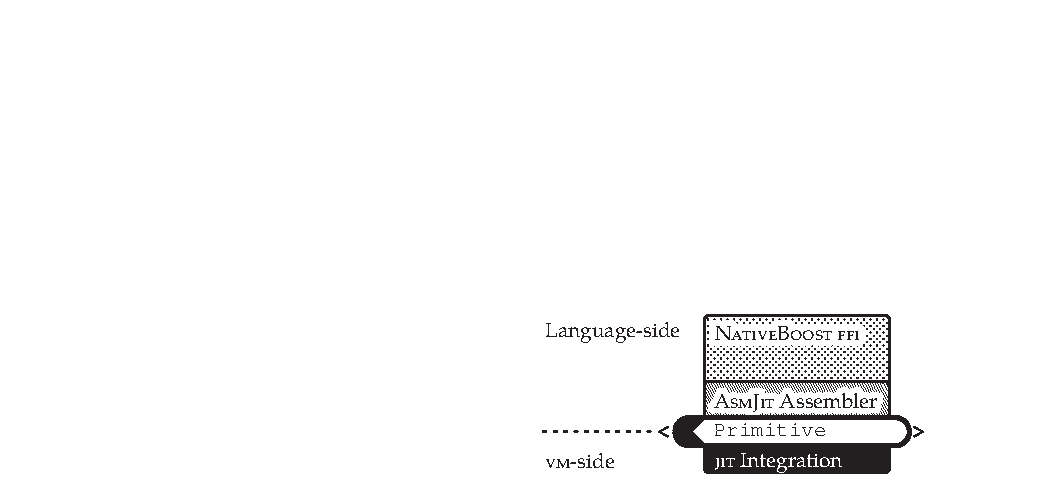
\includegraphics[scale=1.1]{nbArchitecture}
	\caption[\NB Components Layering]{\NB main components that major part of the code resides at language-side.}
	\figlabel{ffi-nbArchitecture}
\end{figure}

% General \FFI overview and difference of NB
\begin{figure*}[t]
	\centering
	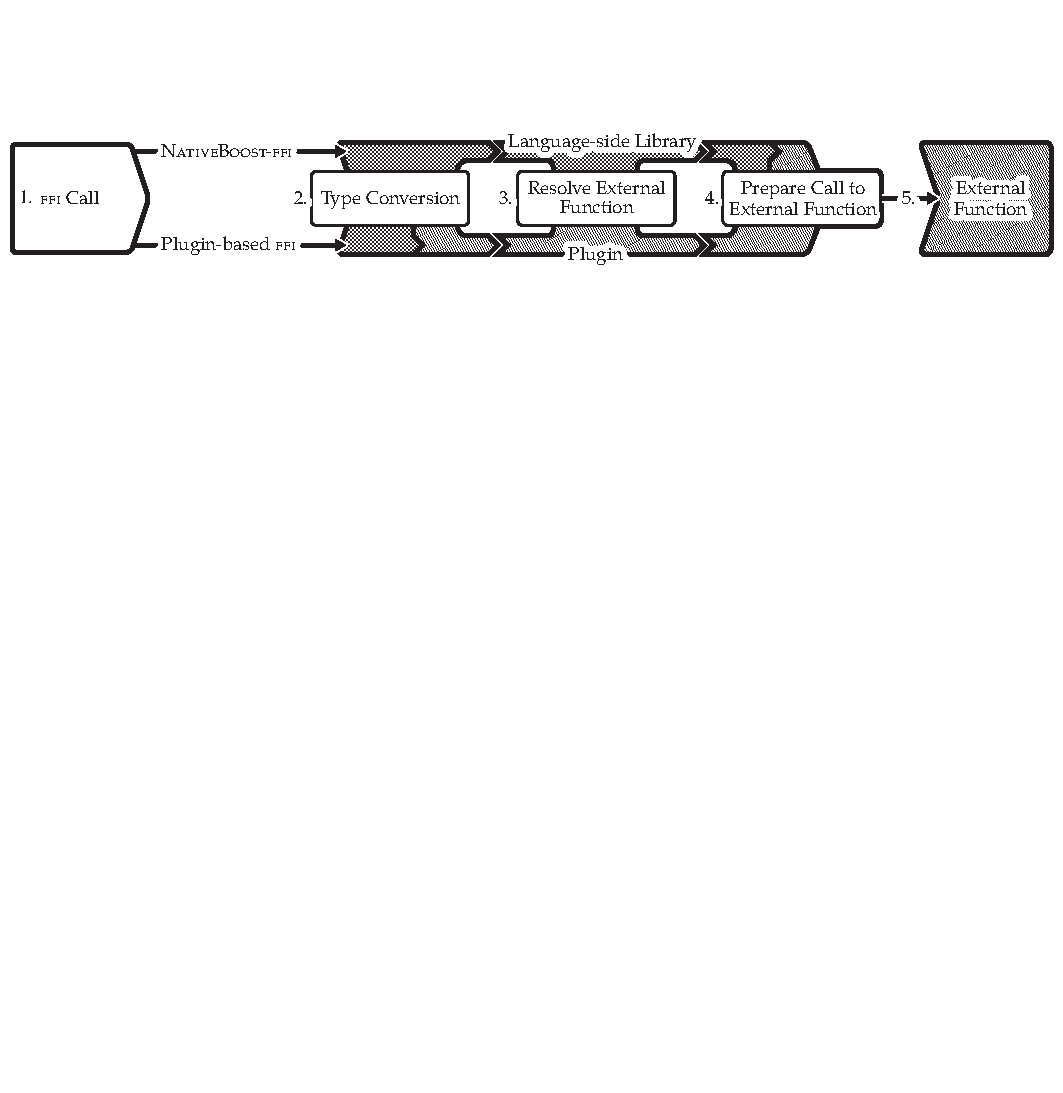
\includegraphics[width=\textwidth]{ffiOverview}
	\caption[\FFI Implementation Comparison]{Comparison of \FFI calls propagation in \NBFFI and a typical \VM plugin-based implementation. \NB resorts to \VM-level only for the native-code activation, whereas typical implementations cross this barrier much earlier.}
	\figlabel{ffi-ffi}
\end{figure*}

\paragraph{Callout propagation.}
\figref{ffi-ffi} shows a comparison of the resolution of a \FFI call both in \NBFFI and a plugin-based \FFI.
At step 1, a \FFI call is emitted.
The \NBFFI call is mostly processed at language-side and it is only during step 4 that a primitive is called and the \VM effectively does the external call by executing the native code.
On the opposite, a plugin-based \FFI call already crossed the low-level frontier in step 2 resulting that part of the type conversion process (marshalling) is already done in the \VM code.
In \NBFFI, doing most of the \FFI call processing at language-side makes easier to keep control, redefine or adapt it if needed.

% ===========================================================================
\section{\NBFFI Evaluation}
\seclabel{ffi-evaluation}
% ===========================================================================

In this section we compare \NB with other \FFI implementations.
\begin{description}
	\item[\Alien \FFI:] An \FFI implementation for Squeak/\PH that focuses on the language-side. All marshalling happens transparently at language-side.
	\item[C-\FFI:] A C based \FFI implementation for Squeak/\PH that performs all marshalling operations at \VM-side.
	\item[\LuaJIT:] A fast \Lua implementation that has a close \FFI integration with \JIT interaction.
\end{description}

\paragraph{Choice of \FFI Implementations.}
To evaluate \NB we explicitly target \FFI implementations running on the same platform, hence we can rule out additional performance differences.
\Alien and C-\FFI run in the same \PH image as \NB allowing a much closer comparison.

\Alien \FFI is implemented almost completely at language-side, much like \NB.
However, as the following benchmarks will stress, it also suffers from performance loss.

On the other end there is C-\FFI which is faster than \Alien but by far not as flexible.
For instance only primitive types are handled directly.

As the third implementation we chose \Lua which is widely used as scripting language in game development.
Hence much care has been taken to closely integrate \Lua into C and C++ environments.
\LuaJIT integrates an \FFI library that generates the native code for marshalling and directly inlines C functions callout in the \JIT-compiled code.

\paragraph{Evaluation Procedure.}
To compare the different \FFI approaches we measure 100 times the accumulative time spent to perform $1'000'000$ callouts of the given function.
From the 100 probes we show the average and the standard deviation for a $68\%$ confidence interval in a gaussian distribution.
To exclude the calling and loop overhead we subtract from each evaluation the time spent in the same setup, but without the \FFI call.
The final deviation displayed is the arithmetic average of the measured deviation of the base and the callout measurement.

The three \ST \FFI solutions (\NB, \Alien, C-\FFI) are evaluated on the very same \PH 1.4 (version 14458) image on a \PH \VM (version of May 5. 2013).
For the \Lua benchmarks we use \LuaJIT 2.0.1.
The benchmarks are performed under the constant conditions on a MacBook Pro.
Even though a standalone machine could improve the performance we are only interested in the relative performance of each implementation.


\paragraph{Choice of Callouts.}
We chose a set of representative C functions to stress different aspects of an \FFI implementation.
We start with simple functions that require little marshalling efforts and thus mainly focus on the activation performance and callout overhead.
Later we measure more complex C functions that return complex types and thus stress the marshalling infrastructure.

% ---------------------------------------------------------------------------
\subsection{Callout Overhead}
% ---------------------------------------------------------------------------

The first set of \FFI callouts show mainly the overhead of the \FFI infrastructure to perform the callout.

For the first \FFI evaluation we measure the execution time for a \ttt{clock()} callout.
The C function takes no argument and returns an integer thus guaranteeing a minimal overhead for marshalling and performing the callout.
%
\begin{table}[H]
    \centering
    \begin{tabular}{rlr}
                    & Call Time                         & Relative Time \\\midrule
        \NB         & \ttt{492.13} $\pm$ \ttt{0.73} ms  & $1.0 \times$ \\
        \Alien       & \ttt{606.6 } $\pm$ \ttt{1.9 } ms  & $\approx 1.2\times$ \\
        C-\FFI       & \ttt{541.77} $\pm$ \ttt{0.88} ms  & $\approx 1.1\times$ \\
        \LuaJIT      & \ttt{343.0 } $\pm$ \ttt{1.2 } ms  & $\approx 0.7\times$
    \end{tabular}
    \caption{Speed comparison of an \ttt{uint clock(void)} \FFI call (see Code~\lstref{ffi-clock}).}
    \tablabel{ffi-performance-clock}
\end{table}
%
\noindent \ttt{abs} is a about the same complexity as the \ttt{clock} function, however accepting a single integer as argument.
%
\begin{table}[h!]
    \centering
    \begin{tabular}{rlr}
                    & Call Time                           & Relative Time \\\midrule
        \NB         & \ttt{ 65.34 } $\pm$ \ttt{0.23 } ms  & $1.00 \times$ \\
        \Alien       & \ttt{175.77 } $\pm$ \ttt{0.31 } ms  & $\approx 2.69\times$ \\
        C-\FFI       & \ttt{148.77 } $\pm$ \ttt{0.21 } ms  & $\approx 2.27\times$ \\
        \LuaJIT\tablefootnote{Downsampled from increased loop size by a factor $100$ to guarantee accuracy.}
                    & \ttt{  }\ttt{  2.035} $\pm$ \ttt{0.015} ms  & $\approx 0.03\times$
    \end{tabular}
    \caption{Speed comparison of an \ttt{int abs(int i)} \FFI call (see \figref{ffi-nativeBoostSyntax}).}
    \tablabel{ffi-performance-abs}
\end{table}


\paragraph{Evaluation.}
For measuring the calling overhead we chose the \ttt{abs} \FFI callout.
This C function is completed in a couple of instructions which in comparison to the conversion and activation effort of the \FFI callout is negligible.
In \tabref{ffi-performance-abs} we see that \NB is at least a factor two faster than the other \ST implementation.
Yet \LuaJIT outperform \NB by an impressive factor 30.
\LuaJIT has a really close integration with the \JIT and this is what makes the impressive \FFI callout results possible.


% ---------------------------------------------------------------------------
\subsection{Marshalling Overhead for Primitive Types}
% ---------------------------------------------------------------------------

The third example calls \ttt{getenv('PWD')} expecting a string as result:  the path of the current working directory.
Both argument and result have to be converted from high-level strings to C-level zero-terminated strings.
%
\begin{table}[h!]
    \centering
    \begin{tabular}{rlr}
                    & Call Time                          & Relative Time \\\midrule
        \NB         & \ttt{ 105.29} $\pm$ \ttt{0.24} ms  & $1.0 \times$ \\
        \Alien      & \ttt{1058.7 } $\pm$ \ttt{2.0 } ms  & $\approx 10.1\times$ \\
        C-\FFI      & \ttt{ 282.94} $\pm$ \ttt{0.24} ms  & $\approx 2.7\times$ \\
        \LuaJIT\tablefootnote{Downsampled from increased loop size by a factor $10$ to guarantee accuracy.}
                    & \ttt{ }\ttt{ 97.3 } $\pm$ \ttt{5.1 } ms  & $\approx 0.9\times$
    \end{tabular}
    \caption{Speed comparison of an \ttt{char * getenv(char *name)} \FFI call (see Code \lstref{ffi-getenv}).}
    \tablabel{ffi-performance-getenv}
\end{table}

\noindent As a last evaluation of simple C functions with \NB, we call \ttt{printf} with a string and two integers as argument.
The marshalling overhead is less than for the previous \ttt{getenv} example.
However, \ttt{printf} is a more complex C function which requires more time to complete: it has to parse the format string, format the given arguments and pipe the results to standard out.
Hence the relative overhead of an \FFI call is reduced.
%
\begin{table}[h!]
    \centering
    \begin{tabular}{rlr}
                    & Call Time                          & Relative Time \\\midrule
        \NB         & \ttt{ 371.03} $\pm$ \ttt{0.51} ms  & $1\times$ \\
        \Alien      & \ttt{1412.37} $\pm$ \ttt{0.79} ms  & $\approx 3.8\times$ \\
        C-\FFI      & \ttt{ 605.02} $\pm$ \ttt{0.23} ms  & $\approx 1.6\times$ \\
        \LuaJIT     & \ttt{ 202.4 } $\pm$ \ttt{2.1 } ms  & $\approx 0.6\times$
    \end{tabular}
    \caption{Speed comparison of an \ttt{int printf(char *name, int num1, int num2)} \FFI call}
    \tablabel{ffi-performance-printf}
\end{table}

\paragraph{Evaluation.}
\tabref{ffi-performance-clock} and \tabref{ffi-performance-abs} call C functions that return integers for which the conversion overhead is comparably low.
However we see that \Alien compares worse in the case of more complex Strings.
\tabref{ffi-performance-getenv} and \tabref{ffi-performance-printf} show this behavior.
For the \ttt{getenv} a comparably long string is returned which causes a factor 10 conversion overhead for \Alien.


% ---------------------------------------------------------------------------
\subsection{Using Complex Structures}
% ---------------------------------------------------------------------------

To evaluate the impact of marshalling complex types, we measure the execution time for a callout to \ttt{cairo\_matrix\_multiply}.
In all cases, the allocation time of the structs is not included in the measurement nor their field assignments.
\tabref{ffi-performance-structs} shows the results.

\begin{table}[h!]
    \centering
    \begin{tabular}{rlr}
                    & Call Time                         & Relative Time \\\midrule
        \NB         & \ttt{ 79.00} $\pm$ \ttt{0.27} ms  & $1.0\times$ \\
        \Alien      & \ttt{753.82} $\pm$ \ttt{0.51} ms  & $\approx 9.5\times$ \\
        C-\FFI      & \ttt{380.8 } $\pm$ \ttt{2.7 } ms  & $\approx 3.6\times$ \\
        \LuaJIT     & \ttt{ }\ttt{ 5.66} $\pm$ \ttt{0.15} ms  & $\approx 0.07\times$
    \end{tabular}
    \caption{Speed comparison of an \ttt{cairo\_matrix\_multiply} \FFI call (cf. \lstref{ffi-cairoCallouts})}
 	\tablabel{ffi-performance-structs}
\end{table}

\paragraph{Evaluation.}
In \tabref{ffi-performance-structs} shows that \NB outperforms the two other \ST implementations.

% ---------------------------------------------------------------------------
\subsection{Callbacks}
% ---------------------------------------------------------------------------

\tabref{ffi-performance-qsort} shows a comparison of \ttt{qsort} callouts passing callbacks.
Callbacks are usually much more slower than callouts.

\begin{table}[H]
    \centering
    \begin{tabular}{rlr}
                    & Call Time                          & Rel. Time \\ \midrule
        \NB         & \ttt{2300.0 } $\pm$ \ttt{1.1 } ms  & $ 1.0 \times$ \\
        \Alien      & \ttt{ 600.83} $\pm$ \ttt{0.35} ms  & $\approx 0.26 \times$ \\
        C-\FFI      & NA                                 & NA \\
        \LuaJIT     & \ttt{ }\ttt{ 46.13} $\pm$ \ttt{0.62} ms  & $\approx 0.02 \times$\\
		\cmidrule(r){2-3}
	\NB \small{with}
	   \small{Native Callbacks}    & \ttt{ }\ttt{ }\ttt{ 4.98} $\pm$ \ttt{0.21} ms  & $\approx 0.002 \times$
    \end{tabular}
    \caption{Speed comparison of a \ttt{qsort} \FFI call (cf. \lstref{ffi-calloutWithCallback})}
 	\tablabel{ffi-performance-qsort}
\end{table}


\paragraph{Evaluation.}
The results show that \NB callbacks are currently slower than \Alien's ones.
This is because \Alien relies on specific \VM support for callbacks making their activation faster (context creation and stack pages integration).
On the opposite, \NB currently uses small support from the \VM side and even do part of the work at image side.
This \ttt{qsort} demonstrates the worst case because it implies a lot of activations of the callback.
For each of these calls, \NB creates a context and make the \VM switch to it.
To really demonstrate that these context switches are the bottleneck, \tabref{ffi-performance-qsort} also shows the result of doing the same benchmark in \NB but using a native callback i.e. containing native code.
We do not argue here that callbacks should be implemented in native code but that \NB support for callback can be optimized to reach \Alien's performance at least.

% ===========================================================================
\section{\NBFFI Implementation Details}
\seclabel{ffi-internals}
% ===========================================================================
\todo{Check that we don't have too much overlap with the Benzo Chapter}

The following subsections will first focus on the high-level, language-side aspects of \NB, such as native code generation and marshalling.
As a second part we describe implementation details of the low-level extensions, such as the \NB primitives and the \JIT interaction.

% ---------------------------------------------------------------------------
\subsection{Generating Native Code}
\seclabel{ffi-generating}
% ---------------------------------------------------------------------------

In \NB all code generation happens transparently at language-side.
The various examples shown in \secref{ffi-nutshell} show how an \FFI callout is defined in a standard method.
Upon first activation the \NB primitive will fail and by default continues to evaluate the following method body.
This is the point where \NB generates native code and attaches it to the compiled method.
\NB then reflectively resends the original message with the original arguments (for instance \ttt{abs:} in the example \figref{ffi-nativeBoostSyntax}).
On the second activation, the native code is present and thus the primitive will no fail but run the native code.
\secref{ffi-nbPrimitive} will give more internal details about the code activation and triggering of code generation.

% ---------------------------------------------------------------------------
\paragraph{Generating Assembler Instructions}

\figref{ffi-nbArchitecture} shows that \NB relies on AsmJit\footnote{\url{http://smalltalkhub.com/\#!/~Pharo/AsmJit}}, a language-side assembler.
AsmJit emerged from an existing C++ implementation\footnote{\url{https://code.google.com/p/asmjit/}} and currently supports the x86 instruction set.

In fact it is even possible to inline custom assembler instructions in \PH when using \NB.
This way it is possible to meet critical performance requirements.
Typically \ST does not excel at algorithmic code since such code does not benefit from dynamic message sends.

% ---------------------------------------------------------------------------
\paragraph{Reflective Symbiosis}

\NB lives in symbiosis with the \PH programming environment.
As shown in the examples in \secref{ffi-nutshell} and in more detail in \figref{ffi-nativeBoostSyntax} \NB detects which method arguments correspond to which argument in the \FFI callout.
To achieve this, \NB inspects the activation context when generating native code.
Through reflective access to the execution context we can retrieve the method's source code and thus the argument names and positions.

% ---------------------------------------------------------------------------
\paragraph{Memory Management}

\todo{strip BENZO duplication}

\NB supports external heap management with explicit allocation and freeing of memory regions.
There are interfaces for \ttt{allocate} and \ttt{free} as well as for \ttt{memcopy}:
%
\begin{stcode}[
	label={lst:ffi-externalHeap},
	caption={Example of external heap management in \NB}]{0}
memory := NativeBoost allocate: 4.
bytes  := #[1 2 3 4].
"Fill the external memory"
NativeBoost memCopy: bytes to: memory size: 4.

"FFI call to fill the external object"
self fillExternalMemory: memory.

"Copy back bytes from the external object"
NativeBoost memCopy: memory to: bytes size: 4.
NativeBoost free: memory.
\end{stcode}

Using the external heap management it is possible to prepare binary blobs and structures for \FFI calls.

In the previous example Code \lstref{ffi-externalHeap} the \ttt{memory} variable holds a wrapper for the static address of the allocated memory.
Hence accessing it from low-level code is straight forward.
However in certain situations it is required to access a high-level object from assembler.
\PH has a moving garbage collector which means that you can not refer directly to a high-level object by a fixed address.

\begin{figure}[h]
	\centering
	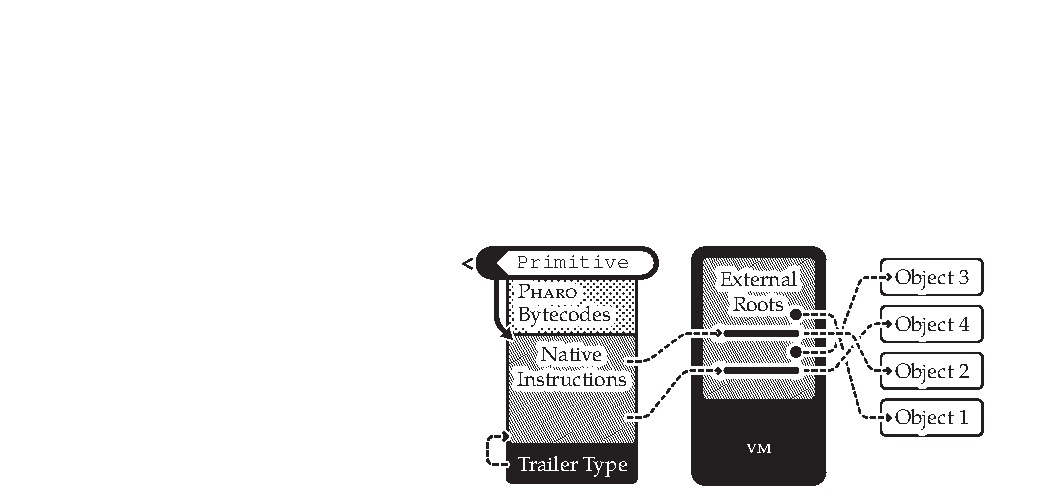
\includegraphics{externalRoots}
	\caption[\NBFFI External Roots]{\todo{duplicate and minor importance here, refer to section in benzo chapter}Pointers in a \ttt{CompiledMethod} to objects registered as external roots are pinpointed at fixed offset in global \VM-level object.}
	\figlabel{ffi-externalRoots}
\end{figure}

To deal with this problem the \VM has a special array at a known address that contains pointers to high-level objects.
The garbage collector keeps this external roots array up to date.
Hence it is possible to statically refer to a \PH object using a double indirection over the external roots.
\figref{ffi-externalRoots} visualizes how native code directly accesses \PH objects through this indirection.


% ---------------------------------------------------------------------------
\subsection{Activating Native Code}
% ---------------------------------------------------------------------------

In this section we present the \VM-level interaction of \NB.
Even though \NB handles most tasks directly at language-side it requires certain changes on \VM level:
\begin{itemize}
	\item executable memory,
	\item activation primitives for native code.
\end{itemize}
%
Since \NB manages native code at language-side there is no special structure or memory region where native code is stored.
Native instructions are appended to compiled methods which reside on the heap.
Hence the heap has to be executable in order to jump to the native instructions.


% ---------------------------------------------------------------------------
\paragraph{The \NB activation Primitive}
\seclabel{ffi-nbPrimitive}

\todo{strip BENZO duplication: see how much overlaps, only put a small summary here and push detailed explanation to the benzo chapter}

In \secref{ffi-generating} we explained how \NB creates \FFI callouts at language-side.
However, so far we left out the part on how the generated native code is activated.

The examples in \secref{ffi-nutshell}, especially \figref{ffi-nativeBoostSyntax} show that each \NBFFI callout requires a special primitive.
\figref{ffi-nativeCodeActivation} shows how a \NB method is activated.


\begin{figure}[h]
	\centering
	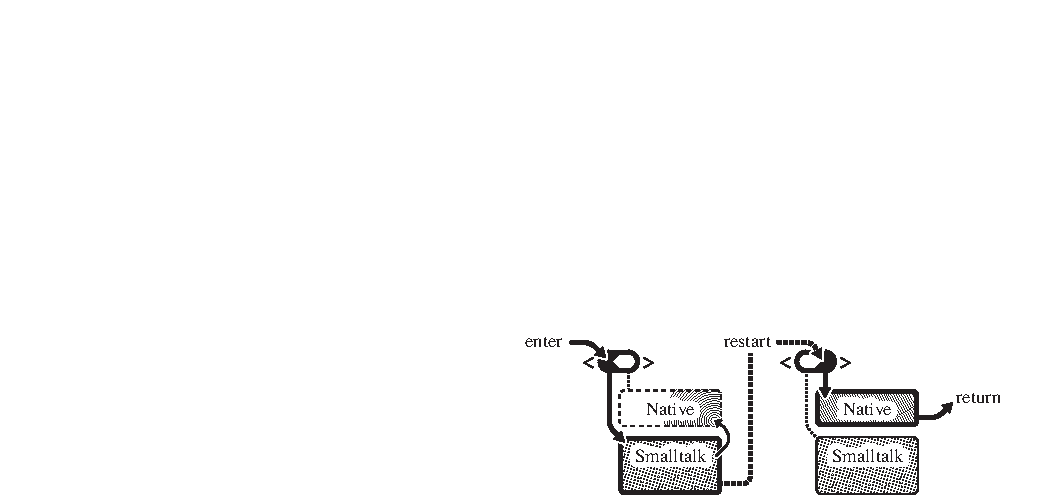
\includegraphics[scale=1.1]{nativeCodeActivation}
	\caption[\NB Native Code Activation]{\todo{Add Primitive Failure Arrow + link to NB code generation}Native code activation. The first call triggers the code generation. Then the method is restarted and the native code executed.}
	\figlabel{ffi-nativeCodeActivation}
\end{figure}

\begin{itemize}
\item In the first step (cf. \ding{182}) the \NB callout primitive is activated.
	The primitive checks if the compiled method actually contains native code.
\item On the first activation there is no native code available yet.
	Hence the primitive will fail and the \ST body (cf. \ding{183}) of the \NB method gets evaluated.
	This is where \NB prepares the native code for the \FFI callout.
\item After installing the native code in the method trailer, the \NB method is reactivated with the original arguments (cf. \ding{184}).
\item Again we end up in the \NB activation primitive (cf. \ding{185}).
	However, this time there is native code (cf. \ding{186}) available and thus the primitive jumps to the native code instead.
\end{itemize}

% ===========================================================================
\section{Related Work}
\seclabel{ffi-relatedWork}
% ===========================================================================
\todo{only show \FFI related work here! all the abstract implementations are covered in the Benzo secrtion}

% other less related approaches: Python ctypes ? SWIG ?

Typical \ST system are isolated from the low-level world and provide only limited interoperability with C libraries.
However there are notable exceptions: \textsc{Étoilé} and \ST/X.

Chisnall presents the Pragmatic \ST Compiler \cite{Chis12a}, part of the \textsc{Étoilé} project, which focuses on close interaction with the C world.
The main goal of this work is to reuse existing libraries and thus reduce duplicated effort.
The author highlights the expressiveness of \ST to support this goal.
In this \ST implementation multiple languages can be mixed efficiently.
It is possible to mix Objective-C, \ST code.
All these operations can be performed dynamically at runtime.
Unlike our approach, \textsc{Étoilé} aims at a complete new style of runtime environment without a \VM.
Compared to that, \NB is a very lightweight solution.


Other dynamic high-level languages such as \Lua leverage \FFI performance by using a close interaction with the \JIT.
\LuaJIT\footnote{\url{https://github.com/jmckaskill/luaffi}} for instance is an efficient \Lua implementation that inlines \FFI calls directly into the \JIT compiled code.
Similar to \NB this allows one to minimize the constant overhead by generating custom-made native code.
The \LuaJIT runtime is mainly written in C which has clearly different semantics than \Lua itself.


On a more abstract level, high-level low-level programming \cite{Fram09a} encourage to use high-level languages for system programming.
Frampton et al. present a low-level framework  which is used as system interface for \Jikes, an experimental \Java \VM.
%Additionally their framework is successfully used in MMTK \cite{Blac04a} which is used independently in several other projects.
%The \ttt{org.vmmagic} package is much more elaborate than \NB but it is tailored towards Java with static types.
However their approach focuses on a static solution.
Methods have to be annotated to use low-level functionality.
Additionally the strong separation between low-level code and runtime does not allow for reflective extensions of the runtime.
Finally, they do not support the execution and not even generation of custom assembly code on the fly.


Kell and Irwin \cite{Kell11a} take a different look at interacting with external libraries.
They advocate a Python \VM that allows for dynamically shared objects with external libraries.
It uses the low-level \textsc{dwarf} debugging information present in the external libraries to gather enough metadata to automatically generate \FFIs.

% ===========================================================================
\section{Problems}
\seclabel{ffi-problems}
% ===========================================================================
\todo{most problems overlap with the problems mentioned in the Benzo chapter} \\
\todo{address problems on a more high-level view}


\subsection{Difficult Debug Cycles}
\todo{debugging facility (on a higher level than Benzo, see invisible \VMs)} \\
\todo{resolve C symbols} \\
\todo{show C source code?} \\
\todo{Compare with luajit-ffi}


\subsection{Platform Independence}
\todo{general / direct dependence on assembler which is not good} \\
\todo{partial platform indepencen with platform-id is guaranteed}
\todo{low-level platform independence solved by Benzo (link to future reference to VirtualCPU)} \\
\todo{platform independence on function level (see OSEnvironment as an Example)} \\
\todo{	- requires explicit subclasses} \\
\todo{	- manual maintenance + singletons} \\
\todo{missing support for multi-platform code definition in a single method}


\subsection{Limited Expressiveness}
\todo{fork example is hard to achieve (vm is not directly forkable)} \\
\todo{current design makes it difficult to perform more C-like operations in one run} \\
\todo{adopt benzo-level abstractions on VirtualCPU}


\subsection{Bootstrap Recursion}
\todo{What happens when using \FFI in bootstrap critical applications?}

% ===========================================================================
\section{Future Work}
\seclabel{ffi-futurework}
% ===========================================================================
Even though \NB shows good overall performance when it comes to callbacks it does not keep up with other \ST-based solutions.
In the current development phase not much attention was payed to callback performance as it is not a common use case for \FFI callouts.
Fast callbacks require close interaction and specific modifications at \VM-level.
However, initially \NB kept the modifications to the \VM at a minimum.
We assume that we can reach the same performance as \Alien relying on the same low-level implementation.

As a second issue we would like to address the callout overhead by using an already existing \JIT integration of \NB.
Currently the \VM has to leave from \JIT-mode to standard interpretation mode when it activates an \NB method.
This context switch introduces an unnecessary overhead for an \FFI callout.
A current prototype directly inlines the native code of a \NB method in the \JIT.
Hence the cost for the context switch plus the cost of activating the \NB callout primitive can be avoided.
% \lf{This modification aims at better integrating \NB and the \JIT such as it is done in LuaJIT.}



% ===========================================================================
\section{Conclusion}
\seclabel{ffi-conclusion}
% ===========================================================================
\todo{make proper summary}
In this paper we presented \NB a novel approach to foreign function interfaces.
Our approach relies only on a very generic extension of the \VM to allow for language-side code to directly call native instructions.

Using a in depth evaluation of \NB comparing against two other \ST \FFI implementations and \LuaJIT we showed in \secref{ffi-evaluation} that our language-side approach is competitive.
\NB reduces the callout overhead by more than a factor two compared to the two closest \ST solutions.

Compared to \LuaJIT there is still space for improvements.
We measured a factor 30 lower calling overhead due to a close \JIT integration.
However for typical \FFI calls the absolute time difference between \NB and \Lua is roughly $30\%$.
With a partial solution ready to integrate \NB closer with the \JIT we expect to come close to \Lua's performance.

Furthermore we showed that \NB essentially combines \VM-level performance with language-side flexibility when it comes to marshal complex types.
New structures are defined practically at language-side and conversion optimizations are added transparently.

% =============================================================================
\ifx\wholebook\relax\else
    \end{document}
\fi

\documentclass[a4paper,12pt,twoside]{../includes/ThesisStyle}
\usepackage[utf8]{inputenc}
\usepackage[T1]{fontenc}

\usepackage[left=1.5in,right=1.3in,top=1.1in,bottom=1.1in,includefoot,includehead,headheight=13.6pt]{geometry}\renewcommand{\baselinestretch}{1.05}


% =============================================================================
%\usepackage[sectionbib]{chapterbib}	% Cross-reference package (Natural BiB)
%\usepackage{bibunits}
%\usepackage{natbib}					% Put References at the end of each chapter
\usepackage{algorithm}
\usepackage{alltt}
\usepackage{amsfonts}
\usepackage{amsmath}
\usepackage{amssymb}
\usepackage{cite}
\usepackage{color}
\usepackage{enumerate}
\usepackage{booktabs} % used for \midrule
\usepackage{fancyhdr}					% Fancy Header and Footer
\usepackage{graphicx}
\usepackage{ifthen}
\usepackage{latexsym}
\usepackage{multirow}
\usepackage{rotating}					% Sideways of figures & tables
\usepackage{stmaryrd}
\usepackage{subfigure}
\usepackage{url}         
\usepackage{xspace}
\usepackage[normalem]{ulem} % for \sout
\usepackage{xcolor}
\usepackage{tablefootnote}
\usepackage{pifont}

% =============================================================================

% Table of contents for each chapter
\usepackage[nottoc, notlof, notlot]{tocbibind}
\usepackage{minitoc}
\setcounter{minitocdepth}{1}
\mtcindent=15pt

\setcounter{secnumdepth}{3}
\setcounter{tocdepth}{2}
  
% =============================================================================
% Fancy Header Style Options

\pagestyle{fancy}                       % Sets fancy header and footer
\fancyfoot{}                            % Delete current footer settings

%\renewcommand{\chaptermark}[1]{         % Lower Case Chapter marker style
%  \markboth{\chaptername\ \thechapter.\ #1}}{}} %

%\renewcommand{\sectionmark}[1]{         % Lower case Section marker style
%  \markright{\thesection.\ #1}}         %

\fancyhead[LE,RO]{\bfseries\thepage}    % Page number (boldface) in left on even
% pages and right on odd pages
\fancyhead[RE]{\bfseries\nouppercase{\leftmark}}      % Chapter in the right on even pages
\fancyhead[LO]{\bfseries\nouppercase{\rightmark}}     % Section in the left on odd pages

\let\headruleORIG\headrule
\renewcommand{\headrule}{\color{black} \headruleORIG}
\renewcommand{\headrulewidth}{1.0pt}
\usepackage{colortbl}
\arrayrulecolor{black}

\fancypagestyle{plain}{
  \fancyhead{}
  \fancyfoot{}
  \renewcommand{\headrulewidth}{0pt}
}


% =============================================================================
% Clear Header Style on the Last Empty Odd pages
\makeatletter

\def\cleardoublepage{\clearpage\if@twoside \ifodd\c@page\else%
  \hbox{}%
  \thispagestyle{empty}%              % Empty header styles
  \newpage%
  \if@twocolumn\hbox{}\newpage\fi\fi\fi}

\makeatother

\newenvironment{maxime}[1]
{
\vspace*{0cm}
\hfill
\begin{minipage}{0.5\textwidth}%
%\rule[0.5ex]{\textwidth}{0.1mm}\\%
\hrulefill $\:$ {\bf #1}\\
%\vspace*{-0.25cm}
\it 
}%
{%

\hrulefill
\vspace*{0.5cm}%
\end{minipage}
}

\let\minitocORIG\minitoc
\renewcommand{\minitoc}{\minitocORIG \vspace{1.5em}}


\renewcommand{\epsilon}{\varepsilon}

% centered page environment
\newenvironment{vcenterpage}
	{\newpage\vspace*{\fill}\thispagestyle{empty}\renewcommand{\headrulewidth}{0pt}}
	{\vspace*{\fill}}
	

%=============================================================================

\usepackage{needspace}
\newcommand{\needlines}[1]{\Needspace{#1\baselineskip}}

\usepackage{xcolor}
\definecolor{source}{gray}{0.95}
% source code formatting
\usepackage{listings}
    % global settings for source code listing package
\lstset{
    basicstyle=\ttfamily\small,
    showspaces=false,
    showstringspaces=false,
    captionpos=b, 
    columns=fullflexible}

\lstdefinelanguage{ST}{
    keywordsprefix=\#,
    morekeywords=[0]{true,false,nil},
    morekeywords=[1]{self,super,thisContext},
    morekeywords=[2]{ifTrue:,ifFalse:,whileTrue:,whileFalse:,and:,or:,xor:,not:,by:,timesRepeat:},
    sensitive=true,
    morecomment=[s]{"}{"},
    morestring=[d]',
    escapechar={!},
    alsoletter={., :, -, =, +, <},
    moredelim=**[is][\itshape]{/+}{+/},
    literate=
        {^}{{$\uparrow$}}1
        {:=}{{$\leftarrow$}}1
        {~}{{$\sim$}}1
        {-}{{\sf -\hspace{-0.13em}-}}1  % the goal is to make - the same width as +
        {+}{\raisebox{0.08ex}{+}}1		% and to raise + off the baseline to match V
        , % Don't forget the comma at the end!
    style=STStyle
}
\lstdefinestyle{STStyle}{
    tabsize=4,
    %frame=leftline,
    % frame=bl,
    %framerule=2pt,
    %rulecolor=\color{gray},
    % backgroundcolor=\color{white},
    %backgroundcolor=\usebeamercolor[bg]{listing},
    basicstyle=\ttfamily\small,
    keywordstyle=\bf\ttfamily,
    % stringstyle=\color{orange},
    stringstyle=\mdseries\slshape,
    commentstyle=\it\rmfamily\color{darkgray}, 
    commentstyle=\mdseries\slshape\color{gray},
    %commentstyle=\mdseries\slshape,
    emphstyle=\bf\ttfamily,
    escapeinside={!}{!},
	%backgroundcolor=\color{source},
    %emphstyle={[2]\color{red}},
    %emphstyle={[3]\color{blue}\bf},
    %emphstyle={[4]\color{blue}},
    keepspaces=true
} 

%\lstnewenvironment{javacode}  [1][]{\lstset{language=java,#1}\needlines{#2}}{} 
%\lstnewenvironment{pythoncode}[2][]{\lstset{language=python,#1}\needlines{#2}}{}
\lstnewenvironment{stcode}    [2][]{\lstset{language=ST,#1}\needlines{#2}}{}
\lstnewenvironment{ccode}     [2][]
    {\lstset{language=C,numbers=left,escapechar=\$,numberstyle=\tiny,#1}\needlines{#2}}{}

% ON: I tried to pass the line number options in as arg #1 but it does not work for me
% I also could net get the line numbers to consistently increase
\lstnewenvironment{numstcode} [2][]
    {\lstset{language=ST,numbers=left,numberstyle=\tiny,numbersep=2pt,#1}\needlines{#2}}{}
\lstnewenvironment{numstcodecont} [2][]
    {\lstset{language=ST,numbers=left,numberstyle=\tiny,numbersep=2pt,firstnumber=last#1}\needlines{#2}}{}

\newcommand{\lst}[1]{{\tt #1}}

% In-line code (literal)

% In-line code (latex enabled)
% Use this only in special situations where \ct does not work
% (within Section headings ...):
\newcommand{\lct}[1]{{\textsf{\textup{#1}}}}
% Code environments
\lstnewenvironment{code}{%
	\lstset{%
		% frame=lines,
		frame=single,
		framerule=0pt,
		mathescape=false
	}
}{}

%\renewcommand{\lstlistingname}{Code Example}

% =============================================================================
\newboolean{showcomments}
\setboolean{showcomments}{true}

\ifthenelse{\boolean{showcomments}} {
	\newcommand{\ugh}[1] {\textcolor{red}{\uwave{#1}}}	% please rephrase
	\newcommand{\ins}[1] {\textcolor{blue}{\uline{#1}}}	% please insert
	\newcommand{\del}[1] {\textcolor{red}{\sout{#1}}}	% please delete
	\newcommand{\chg}[2] {								% please change
		\textcolor{red}{\sout{#1}}{\ra}
		\textcolor{blue}{\uline{#2}}}
	\newcommand{\nbc}[3]{								% comment
		{\colorbox{#3}{\bfseries\sffamily\scriptsize\textcolor{white}{#1}}}
		{\textcolor{#3}{\sf\small$\blacktriangleright$\textit{#2}$\blacktriangleleft$}}}

}{
	\newcommand{\ugh}[1]{#1}							% please rephrase
	\newcommand{\ins}[1]{#1}							% please insert
	\newcommand{\del}[1]{}								% please delete
	\newcommand{\chg}[2]{#2}							% please change
	\newcommand{\nbc}[3]{}								% comment
}

% =============================================================================
\usepackage[pagebackref,hyperindex=true]{hyperref}


% Links in pdf
\usepackage{color}
\definecolor{linkcol}{rgb}{0.0, 0.0, 0.0} 
\definecolor{citecol}{rgb}{0.0, 0.0, 0.0} 

% Change this to change the informations included in the pdf file
% See hyperref documentation for information on those parameters
\hypersetup {
	bookmarksopen=true,
	pdftitle="Design and Use of Anatomical Atlases for Radiotherapy",
	pdfauthor="Olivier COMMOWICK", 
	pdfsubject="Creation of atlases and atlas based segmentation", %subject of the document
	%pdftoolbar=false, % toolbar hidden
	pdfmenubar=true, %menubar shown
	pdfhighlight=/O, %effect of clicking on a link
	colorlinks=true,
	pdfpagemode=UseNone,
	pdfpagelayout=SinglePage,
	pdffitwindow=true,
	linkcolor=linkcol,
	citecolor=citecol,
	urlcolor=linkcol
}

% =============================================================================
\newcommand{\figlabel}[1] {\label{fig:#1}}
\newcommand{\chaplabel}[1]{\label{chap:#1}}
\newcommand{\seclabel}[1] {\label{sec:#1}}
\newcommand{\tablabel}[1] {\label{tab:#1}}
\newcommand{\lstlabel}[1] {\label{lst:#1}}

\newcommand{\figref}[1] {Figure~\ref{fig:#1}}
\newcommand{\chapref}[1]{Chapter~\ref{sec:#1}}
\newcommand{\secref}[1] {Section~\ref{sec:#1}}
\newcommand{\tabref}[1] {Table~\ref{tab:#1}}
\newcommand{\lstref}[1] {Listing~\ref{tab:#1}}

\newcommand{\commented}[1]{}

\newcommand{\bs}    {\symbol{'134}} % backslash
\newcommand{\us}    {\symbol{'137}} % underscore
\newcommand{\ttt}[1]{\texttt{#1}}
\newcommand{\ie}    {\emph{i.e.},\xspace}
\newcommand{\eg}    {\emph{e.g.},\xspace}
\newcommand{\etal}  {\emph{et al.}\xspace}
\newcommand{\ns}    {\!\!\!\!} %big negative space
\newcommand{\cnull} {\textbackslash0\xspace}


\newcommand\fix[1]{\nb{FIX}{#1}}
\newcommand\todo[1]{\nb{TO DO}{#1}}
\newcommand\cb[1]{\nbc{CB}{#1}{purple}}
\newcommand\sd[1]{\nbc{SD}{#1}{orange}}
\newcommand\is[1]{\nbc{IS}{#1}{gray}}
\newcommand\gc[1]{\nbc{GC}{#1}{olive}}
\newcommand\ct[1]{\nbc{CT}{#1}{teal}}
\newcommand\md[1]{\nbc{MD}{#1}{blue}}
\newcommand\dc[1]{\nbc{DC}{#1}{green}}

% =============================================================================
\newcommand{\NBFFI}  {Native\-Boost-FFI\xspace}
\newcommand{\NB}  {Native\-Boost\xspace}
\newcommand{\B}   {Benzo\xspace}
\newcommand{\ST}  {Small\-talk\xspace}
\newcommand{\PH}  {Pharo\xspace}
\graphicspath{{.}{../figures/}}

\begin{document}
% ===========================================================================

\chapter{\B Prototype Application Validation}
\chaplabel{validation}
\minitoc
% ===========================================================================
\introduction
% ===========================================================================

In \chapref{ffi} we presented \NB, a mature language-side \FFI implementation that makes heavy use of \B's infrastructure.
\NB is only one of three applications that are based on \B that were initially outlined in \secref{benzo-usecase}.
While \NB is considered stable, the two other applications are currently only prototypes: dynamic primitives and a language-side \JIT.
Hence we will present the two solutions combined in this chapter.

As first we will present \WF, dynamic primitives based on \B.
\WF takes advantage of the metacircular approach of \PH's \VM and makes the primitive definition available at runtime.
This is a step forward from the typical metacircular approach where the whole reflective power of the host environment can only be used at compile-time.
Once the \VM is compiled, all the high-level definitions that existed at compilation time are no longer accessible from language-side.
\WF tries to make a fraction of the original compile-time definitions accessible.

\todo{probably retrofit to the final results of \NBJ}\enlargethispage{\baselineskip}
The second prototype, \NB a language-side \JIT compiler takes the core idea of \WF even further.
\WF is capable of defining new primitives at runtime which are not reentrant: it is not possible to activate \PH methods from within primitives.
However, this is what happens in jitted methods: it is possible to switch seamlessly between native methods and standard \PH methods using bytecode evaluation.
Much like the primitives, the \JIT can not be changed from language-side and this is where we bring \NBJ into play.
\NBJ reimplements the \VM-level \JIT compiler at language-side and uses \B to install the native code.


% ===========================================================================
%\newpage
\section{\WF: Dynamic Primitives}
\seclabel{val-waterfall}
% ===========================================================================

\begin{figure}[h]
	\centering
	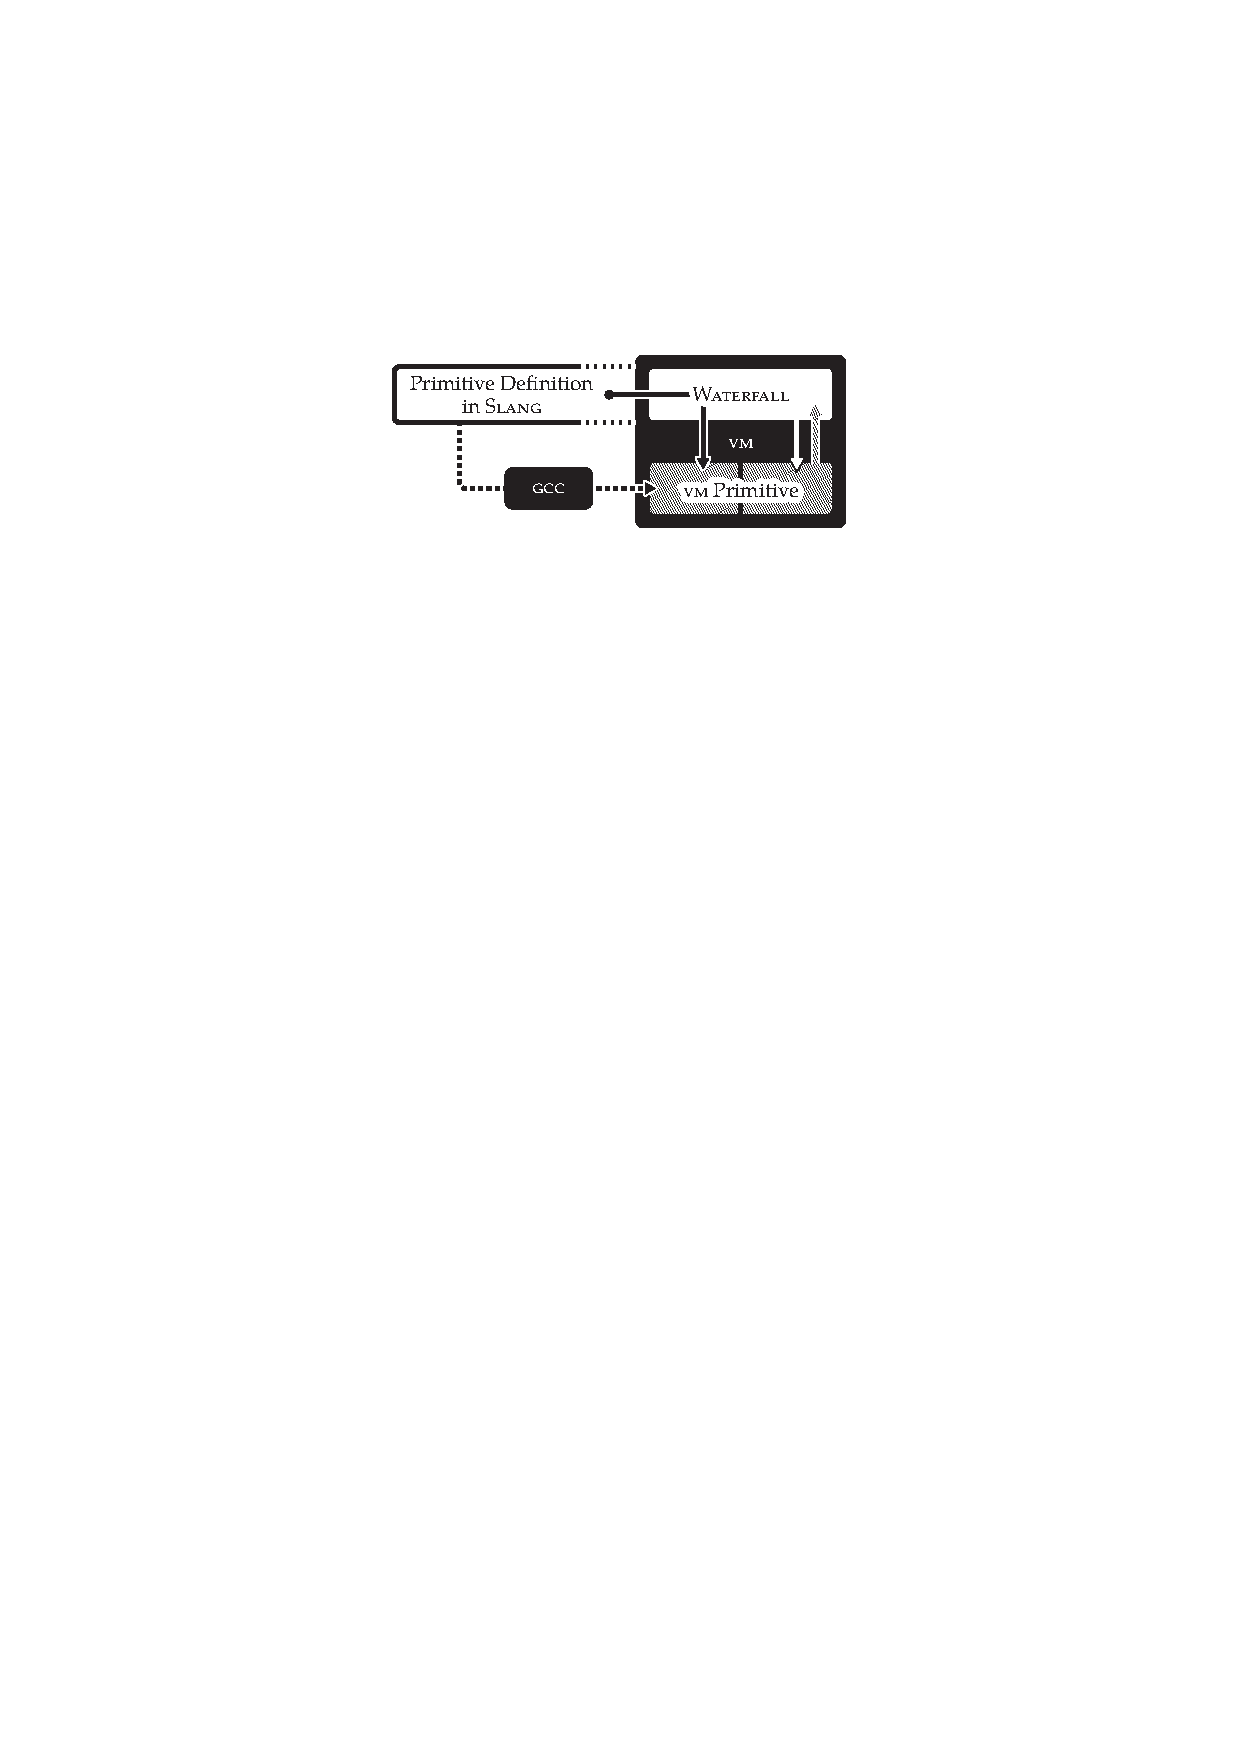
\includegraphics[scale=\imagescale]{waterfall-overview}
	\caption{\WF Overview}
	\figlabel{val-waterfall-overview}
\end{figure}

\noindent In this section we present \WF, a compiler toolchain that allows primitives to be changed dynamically from language-side.
We successfully use \WF to change and recompile whole \VM plugins such as the file plugin as we show in the following \secref{val-waterfall-plugins}.

% -----------------------------------------------------------------------------
\subsection{Background}
\seclabel{val-waterfall-background}
% -----------------------------------------------------------------------------

\WF is our second application on top of \B after \NB, the complete \FFI library previously presented in \chapref{ffi}.
\NB uses \B to generate the glue code between \PH and the external library.
Even though \NB is extendable it is not used to directly synthesize new functionality, the main functionality is defined the external libraries typically written in a low-level language such as C.
Interestingly, the \NB methods containing the callouts behave almost like the existing primitive methods of \PH.
These primitives define a hook into \VM-level native functionality.
In \PH the same mechanism is also used to activate plugins which are again similar to an \FFI callout from language-side.
However, primitives and plugins are statically defined and modifications happen outside \PH.
This is where the domain of \WF begins.

\WF provides infrastructure to dynamically compile and install primitives on top of the \B infrastructure at language-side in \PH.
As we will describe in more detail in the following sections, the \PH \VM is written in a metacircular fashion.
Hence the definition of plugins and primitives can be loaded in standard \PH.
Typically this happens only at compile-time of the \VM, where these definitions are exported to C and compiled to the \VM binary.
Once compiled, the original high-level description of primitives and plugins is no longer accessible from \PH.
As a consequence, existing primitives or plugins can not be changed at runtime.

\WF brings the static primitive definitions to live again.
Just loading the original definitions in \PH does not bring them back to live, even though we can now inspect the definition and browse the sources.
\WF compiles these definitions to native code and installs them with \B as new primitives.
With this infrastructure primitive and plugin modifications are not limited to \VM compilation time.

\paragraph{A Metacircular \VM Written in \Slang}

\WF is implemented in \PH which uses the \urlfootnote{\Cog \VM}{http://www.mirandabanda.org/cogblog/}, originating from the \Squeak \VM\cite{Inga97a}.
The \VM itself is written in a dialect of \ST called \Slang that is essentially limited to the functionality that can be expressed with standard C code.
\Slang serves for two purposes: a high-level C preprocessor, a interactive simulator of the \VM.
The first point has severe consequences.
\Slang basically has the same syntax as \ST but is semantically constrained to expressions that can be resolved statically at compilation or code generation time and are compatible with C.
Hence \Slang's semantics are closer to C than to \ST.
This fact is also visible in the simulator for the \VM.
If \Slang were \ST, separate parts of the \VM could be directly evaluated.
However, since \Slang is bound to C expressions, the simulator sets up a byte array as memory.
The simulated \VM then accesses this byte array as if it were the native memory.

In conclusion we see that the \PH \VM has an abstract representation of the \VM available for simulation.
This abstract representation is then used to generate C sources, already lowering the abstraction level.
After compiling the C sources the original representation of the \VM is not directly accessible anymore.
For instance, even debug symbols are usually stripped from the final binary for performance reasons.
Of course this implies that the \VM can not be changed nor directly inspected from language-side.


\paragraph{Primitives in \PH}
\PH is a highly reflective environment where classes and methods can be changed at runtime, even the current execution context is accessible.
For instance this is used to implement an exception mechanism purely at language-side in \PH.
However, some features can not be implemented at language-side.
\PH uses primitive methods, that instead of evaluating \PH-code switch to a \VM routine.
As already partially explained in \secref{benzo-vm-interaction}, whenever a method is compiled with the \ttt{primitive} pragma as shown a flag is set on the \ttt{CompiledMethod}. 
If the \VM tries to activate such a method, instead of interpreting the bytecodes it calls the corresponding function at \VM-level~\cite{Gold83a}.
We distinguish three categories of primitives based on their functionality: certain parts of the language semantics, \OS-level functionality that can not be implemented in \PH itself and a third less important category where performance is critical.

As we mentioned in the previous paragraph, these primitives are bound to the \VM and can not be changed at runtime.
However, for a certain subset of these primitives we can write language-side substitutes in pure \PH-code.
These primitives are called non-essential and are mainly used for optimization purposes. 
In contrast there are essential primitives which are for instance used during start up of the \PH environment.
Two prominent examples of essential primitives are the ones used for creating new objects or activating a block.

\paragraph{Instrumenting Primitives}
In the context of \WF we are interested in which parts of the system we can modify and thus we draw our attention to these essential primitives.
The only way to modify these primitives is by creating wrappers but that brings a new problem.
Imagine that we wrap around the primitive which creates a new object.
What happens now if the additional wrapper code needs a new object?
It will call the very same primitive that we just wrapped, without protection this causes infinite recursion.
Since technically the wrapper code should live at a different abstraction level than the original primitive we have find our selves mixing meta-levels.

The most radical approach to avoid this meta-recursion is to change the primitive externally.
In the case of \PH this means changing the \Slang sources, exporting and compiling the primitive and restarting the \PH environment on top of this changed \VM.
However, this approach stands in contrast to the reflective nature of \PH where most functionality can be changed at runtime.
Also it is not always suitable to restart the \PH process to modify a small part of the system.

%----------------------------------------------------------------------------
\subsection{\WF's Contribution}
Following the implementation overview of the \PH \VM and the differentiation of different primitives we identify two main benefits of changing \VM primitives at runtime with \WF:

\begin{enumerate}
	\item Reducing \VM complexity by implementing non-essential primitives reflectively at language-side.
	\item Dynamic instrumentation of primitives.
\end{enumerate}

\paragraph{Reducing \VM Complexity}
Low-level \VM extensions are only justified in the presence of strong performance requirements (see \secref{benzo-related}).
All non-essential primitives fall into this category since these primitives can be implemented in \PH without restrictions.
However, in certain cases for performance a language-side implementation is unsuitable.
Additionally we already know that these primitives are available as \Slang code at \VM generation time.
Using \WF, these primitives can be implemented at language-side based on the unmodified \Slang sources.
This means that these primitives become first-class citizens of the high-level environment and thus evolve with less effort.
Thus, \WF opens new possibilities of changing \PH that were previously possible only with significant overhead.

\paragraph{Essential Primitives}
For essential primitives the previous argument does not hold since a static version is needed for a correct startup of the system.
These primitives can not be directly replaced by a language-side implementation using \WF.
Even though \WF itself avoids meta-recursion by generating low-level code with \B.
However, \B itself relies on essential primitives as it is written in \PH.
This imposes certain restrictions how and when these essential primitives can be modified with \WF during system startup.
These restrictions are more related to the underlying \B infrastructure than \WF.
For instance already exposed similar limitations with the \B-based \FFI when used during startup (see \secref{ffi-startup-recursion}).
Nevertheless, nothing prevents from replacing essential primitives at runtime with customized versions, once the system startup is completed. 

\paragraph{Extended Primitive Instrumentation}
Instrumentation of essential primitives from lan\-guage-side is an error-prone task falling in many cases in non-termination due to previously described meta-recursion. 
An example of this behavior, can be observed when changing the essential \ttt{basicNew} primitive, which is responsible for instantiating new objects.
Only very limited instrumentation is possible at language-side, for instance counting how many instances have been created.
This only works since the \VM internally does not represent small integers as full objects.
However, this is only true up to some extent.
Small integers bigger than $2^{30}$ are transformed to a more expensive object representation since they no longer fit in a machine word of the 32-bit \VM. 
These big integers will use the \ttt{basicNew} primitive again as they are not implement in the \VM but in at language-side.
Thus, we are back the original problem of running into meta-recursion.
So even this very simple example has unwanted side-effects that are not directly visible.
More complex instructions tasks will inevitably suffer from the same problems.

Using reflective techniques it is possible to escape from this meta-recursion, however, with a considerable overhead.
\WF avoids these issues since the instrumentation code for primitives will be implemented at the lowest level on top of \B.
In \secref{val-waterfall-performance} we show how \WF, the \B based approach for generating primitives on the fly, outperforms the reflective solutions for primitives instrumentation. 


% -----------------------------------------------------------------------------
\subsection{\WF Implementation}
\seclabel{val-waterfall-implementation}
% -----------------------------------------------------------------------------
\WF uses \B's mechanism for replacing primitive methods with customized versions that are nativized dynamically as described in \chapref{benzo}.
The loophole described there is exploited by \WF to enable dynamic modification of \VM behavior and hence bring primitives to life at language-side.
From a high-level point of view \WF provides two services which work transparently: 

\begin{enumerate}
	\item Compilation of \Slang code on demand (lazily).
	\item A clear interface for executing, at runtime and from language-side, the native code generated.
\end{enumerate}

\noindent The first item allows to change the code of primitives at language-side and generate the corresponding native code when needed. 
It also provides the possibility to write methods or functionality with the same \ST syntax but with a static semantic. 
It consists essentially of a transformation toolchain that transforms the \Slang sources to native code using a \B-based compilation toolchain.

The second item enables the execution of the dynamically generated native code.
This includes for instance the finding of addresses of \VM internal symbols and all the effort to link the two worlds, \ST and native.
\WF relies on \B for most of this low-level functionality.
In particular \NB, the \B-based \FFI presented in \chapref{ffi}, is used for interfacing with C libraries (\ttt{dlsym}). 

% -----------------------------------------------------------------------------
\paragraph{Architecture Overview}
The \WF infrastructure is mainly divided in the following two parts: 
\begin{itemize}[nolistsep,noitemsep]
	\item the installed \Slang sources,
	\item a \B-based compilation toolchain.
\end{itemize}
The \WF compiler transforms the \Slang sources to native code through various transformation steps as show in \figref{waterfall-architecture}.
In order to work properly \WF needs the complete \Slang sources for compilation unit (primitive or plugin) to be loaded upfront.
Once loaded in the \PH image the \AST of the \Slang sources are available which form the input for the \WF compiler.
This means that it is possible to write custom plugins in \PH and transform them using \WF as long as the written \PH code uses the restricted \Slang subset.
As mentioned earlier, the major difference to normal \PH code is the lack of real polymorphism since \Slang is more like C with a \ST syntax.

Technically the \WF compiler takes over the part of the \Slang to C converter and of \GCC in the normal \VM compilation process.
\WF, much like the \Slang to C converter, has to take care of certain type information present in the \Slang sources.
For instance we extract from the type information if arguments are used by value or reference.
With this information we generate native code using a simple stack based strategy for temporary variables.
As for the part of \GCC, \WF in its current state is of course far less complex and the resulting the native code is inferior to \GCC's optimized output.
To simplify the prototype \WF only uses a simple stack strategy instead of register allocation for temporaries.
Additionally \WF does not use intermediate representations (\IR) such as static single assignment (\SSA) to perform elaborate optimizations \cite[Ch.\ 1]{Appe98a}.


% -----------------------------------------------------------------------------
\paragraph{Compilation Steps}
As shown in \figref{waterfall-architecture} the \WF compiler transforms the \AST of the \Slang input to \PH primitives.

\begin{figure}[h]
	\centering
	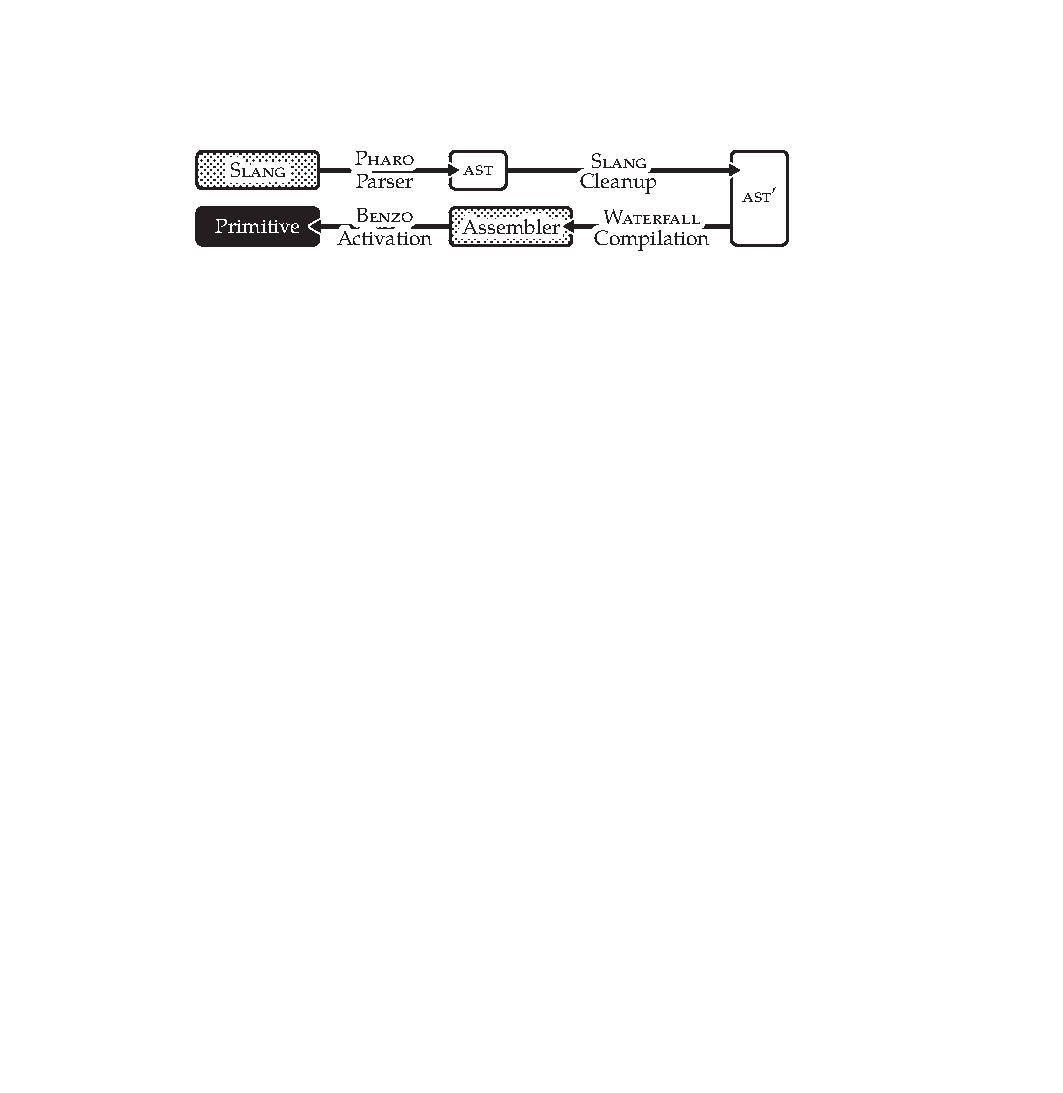
\includegraphics[scale=\imagescale]{waterfall-architecture}
	\caption{\WF Compilation Steps}
	\figlabel{waterfall-architecture}
\end{figure}

\noindent We divide the \WF compiler into four distinct steps:
\begin{description}
\item[\Slang to \AST:] The first step is to access the \AST of the \Slang source method which happens automatically by loading the \Slang code in the \PH image.
At this stage \WF also recursively collects the set of reachable \Slang methods.


\item[\AST Purification:] In a second step certain expressions of the original \Slang \AST are transformed into custom \WF expressions that can be easier transformed later on.
For instance \WF converts C macros that are supported in \Slang which of course only make sense when using a standard C compiler.

\item[\AST to \ASM:] The real native compilation happens in the third step where an \AST-visitor creates assembler instructions using \B's \AsmJIT.
At this point external symbols are statically resolved and directly inlined in the final \ASM code.

\item[\ASM to Primitive] Although not strictly part of the compilation, in the fourth step the final native instructions are installed as a primitive methods using \B (see \secref{benzo-benzo} for more details).
\end{description}


% -----------------------------------------------------------------------------
\paragraph{Dynamically Replacing Primitives}
After explaining the general architecture and the different compilation steps of \WF we shed some light on how the primitives are actually installed.
In reality we rely 100\% on \B for this feature.
Once the native code is generated we transform the target method to a special \B-enabled method that contains the native code.
This procedure is explained in detail in \secref{benzo-benzo} where we show the implementation details of \B.

From a user point-of-view we only have to make sure that the corresponding \Slang sources are available and then hand over that source method to \WF to compile and install it.
Once the installation is complete, the resulting \B-enabled method will contain behave like a \Slang primitive compiled with the original approach using \GCC.

% -----------------------------------------------------------------------------
\paragraph{Dynamically Replacing Plugins}
In \PH there is no real distinction between primitives and plugins as we illustrate with the following code snippets.
The first one depicts an essential primitive to allocate new objects.
The second code example shows the a plugin primitive to open a new file stream.
%
\begin{stcode}[
	caption={\ttt{Object>>\#basicNew} Primitive},
	label={lst:validation-basicnew}]{3}
basicNew
  <primitive: 70>
  OutOfMemory signal.
\end{stcode}
%
\begin{stcode}[caption={\ttt{FilePlugin>>\#open:writeable:} Plugin Primitive}]{5}
open: pathString writable: writableFlag
  "Open a file at the given pathString, and return
   the file ID obtained."
  <primitive: 'primitiveFileOpen' module: 'FilePlugin'>
  ^ nil
\end{stcode}
%
The main difference between primitives and plugins is only how they are distributed.
Primitives are inlined in the \VM and can not be loaded at runtime, while plugins can be loaded dynamically and are bundled separately.
That also means that there is no difference in handling plugins for \WF, the compilation and installation process is exactly the same.

% -----------------------------------------------------------------------------
\subsection{\WF Validation}
\seclabel{val-waterfall-performance}
% -----------------------------------------------------------------------------
After explaining the implementation details of \WF we would like to present a thorough evaluation of the \WF infrastructure.
We split up the validation in two parts following the outlined applications of \WF in the introduction.
The first part describes the performance of \WF when used for instrumenting primitives.
This is the major field of application for \WF as it stresses its dynamic nature.
In contrast to that we evaluate the performance of a \WF compiled plugin in the second part of the validation.
Evaluating a whole plugin puts more stress on the quality of the generated code than the fact that we can dynamically modify primitives.
A more detailed analysis of \WF is also available separately \cite{Char13a}.


% -----------------------------------------------------------------------------
\subsubsection*{Validation of Dynamic Primitives}

In this first part of the \WF validation we compare the performance of \WF generated primitives in \PH.
In the first part we simply measure the speed of a dynamically replaced primitive, while in the second we add instrumentation overhead.
For the simple replacement we choose the simple integer operation "greater than" (\ttt{$>$}) and for instrumentation the more complex \ttt{basicNew} primitive.

\paragraph{Simple Dynamic Primitives}
In this first validation we compare the speed of the \WF generated code on a simple "greater than" primitive.
The primitive is rather simple as it only works on small integers arguments and delegates the functionality for other types to its superclass.
The code for the \ttt{Smallinteger} operation looks as follows.
%
\begin{stcode}{3}
> aNumber
	<primitive: 4>
	^super > aNumber
\end{stcode}
%
The fallback code at the end of the method triggers a slower "greater than" implementation on the super class \ttt{Integer} which mostly deals with the multitude of possible arguments to \ttt{>}.

\begin{stcode}{1}
> aNumber
	aNumber isInteger 
		ifFalse:[
			^ aNumber 
				adaptToInteger: self andCompare: #> ]
	self negative == aNumber negative
		ifFalse: [ ^ aNumber negative ].
	self negative
		ifTrue: [ ^(self digitCompare: aNumber) < 0 ]
		ifFalse: [ ^(self digitCompare: aNumber) > 0 ].
\end{stcode}


\noindent For comparing performance of the "greater than" primitive we use three different approaches:
\begin{enumerate}[noitemsep,nolistsep]
	\item the standard primitive provided by the \VM,
	\item the fallback language-side implementation that is triggered whenever the standard primitive failed,
	\item the reimplementation with \WF (not instrumented).
\end{enumerate}
%
We run the three approaches by measuring the cumulative time over one million primitive activations averaged over $100$ runs.
The absolute numbers are less important than the relative factor between them.
We present the results of this experiment in ~\tabref{val-waterfall-performance}.
%
\begin{table}[H]
    \centering
    \begin{tabular}{rSS}
					& {Running Time [ms]} & {Relative Time} \\\midrule
		Unmodified	&   6.4(14)           & 1.0\\
		Fallback	& 195.0(16)           & \approx30.0 \\
		\WF	        &  22.8(17)           & \approx3.6
    \end{tabular}
    \caption[\WF Speed Comparison: Large Integer]{Comparing running time of different implementations of integer arithmetic primitive.}
    \tablabel{val-waterfall-performance}
\end{table}

\noindent As expected \WF's solution outperforms pure reflective one by factor $9$ to $10$.
\WF clearly outperforms a purely reflective solution since all the meta programming overhead for the intercession mechanism is avoided.
This results thus makes a whole new set of runtime extensions feasible that were previously limited by their strong performance penalty.
Furthermore the performance penalty over a completely optimized \VM solution that has extreme optimization techniques, such as inlining and register allocation, is less than a factor of $4$.

\paragraph{Essential Primitive Instrumentation}
As a second validation target for primitives we chose to instrument \ttt{basicNew} which is a critical primitive for object allocation.
Like the previous "greater than" primitive this belongs to the set of essential primitives that are used during startup of the image.
For instrumentation \ttt{basicNew} is again a rather tricky target as wrong code easily leads to infinite recursion.
However, this can be avoided with a rather costly recursion guard.
We chose a rather simple instrumentation method by simply printing the address of the allocated object to the standard output stream.
We validate the four flavors of the \ttt{basicNew} primitive:
\begin{enumerate}[noitemsep,nolistsep]
	\item the unmodified primitive,
	\item a reflectively instrumented primitive with a recursion guard written in \PH,
	\item a \WF generated and instrumented version,
	\item a \WF generated version without instrumentation.
\end{enumerate}

\noindent We measure again with the same setup as for the previous validation of the "greater than" primitive.
The outcome of this validation is shown in \tabref{val-waterfall-basicnew}.
%
\begin{table*}[h]
    \centering
    \begin{tabular}{rSS}
					                      & {Time [ms]} & {Relative Time} \\\midrule
        Unmodified                        &  0.28(16)           &          1 \\
        Secure reflective instrumentation & 27.72(40)           & \approx 99 \\
        \WF-based instrumentation         &  7.72(27)           & \approx 28 \\
        \WF-based non-instrumentation     &  7.08(23)           & \approx 25 \\
    \end{tabular}
    \caption[\WF Speed Comparison: \ttt{basicNew}]{Slowdown comparison for instrumentation of the  essential primitive \ttt{basicNew}.}
    \tablabel{val-waterfall-basicnew}
\end{table*}
%
Again the results present a similar picture as for the "greater than" validation.
However, since we added instrumentation this time, the reflective \PH is significantly slower than the unmodified version of the primitive.
This proves our theory that in certain performance critical cases reflective solutions are not sufficient.
While we were able to circumvent the recursion problem rather elegantly, the recursion guard is simply too slow to be used by default.
Compared to that, the \WF-based instrumentation is a factor $3$ faster than the reflective solution.
We see that the instrumentation overhead compared to the non-instrumented \WF version is in the range of only $0.7$ms whereas in the \PH version the overhead is several magnitudes higher.
Unlike for the simpler "greater than" primitive \WF is slower: factor $25$ instead of only a factor $3.6$ previously.
This shows that there is certainly room for performance improvements for \WF.

% -----------------------------------------------------------------------------
\subsubsection*{Validation of Dynamic Plugins}
\seclabel{val-waterfall-plugins}

In this second part of the \WF performance evaluation we focus on whole plugins.
Even so we already mentioned that from a language-side point of view there is no difference in plugins and primitives there typically is a significant difference in code size.
While primitives tend to be small and do simple tasks very efficiently (like arithmetic operations) plugins follow a different approach where larger more complex tasks are solved externally.
 
\paragraph{\WF Compiled File Plugin}
\paragraph{\WF Compiled ??? Plugin}
\todo{Write about the File Plugin Validation}\\
\todo{Possibly Validate other plugin}


% -----------------------------------------------------------------------------
\subsection{Problems and Outlook}
% -----------------------------------------------------------------------------

\WF is still a research prototype and thus there are several issues that problems that require attention with the most obvious one being performance.
We have shown that \WF is fast enough to compete against dynamic primitive instrumentation written at language-side, but when compared to native solutions we are still up to two magnitudes slower.
For simplicity \WF currently does not apply any optimizations which still leaves room for improvements.
For instance we do not apply register allocation yet.
However, in our eyes it does not make sense to implement a specific register allocator for \WF itself.
Instead, we envision to use a future platform independent intermediate representation of \B that we presented in \secref{benzo-problems-platform-independence}.
This way most optimizations only require one implementation from which all \B applications benefit.
Using this new \IR would have very little impact on the current \WF compiler infrastructure as we would only have to replace the \AST to \ASM compilation step.
Instead of generating the \ASM we use the \B \IR and let \B generate the native code for the primitives.

\WF is currently only a research prototype that is not used in production.
Also we have seen that there is a significant overlap with the \NB \FFI.
For example, many plugins wrap around existing external libraries and thus are perfect candidates for \NB.
Even though \WF would add a lot of flexibility for such plugins, we believe that \NB is more intention revealing and less confusing that dealing with the semantic differences of \Slang code over \PH code.
Nevertheless, this still leaves the big field of instrumentation open for \WF.
Additionally, for documentation purposes it makes sense to load the \Slang definition of all the essential primitives into the \PH image.
In this case \WF would be a perfect way to bring these primitives to live for exploration purposes.

\todo{better \JIT interaction (leading to the following \NBJ section)}

% ===========================================================================
\newpage
\section{\NBJ: Language-side \JIT Prototype}
\seclabel{val-nabujito}
% ===========================================================================

\begin{figure}[h]
	\centering
	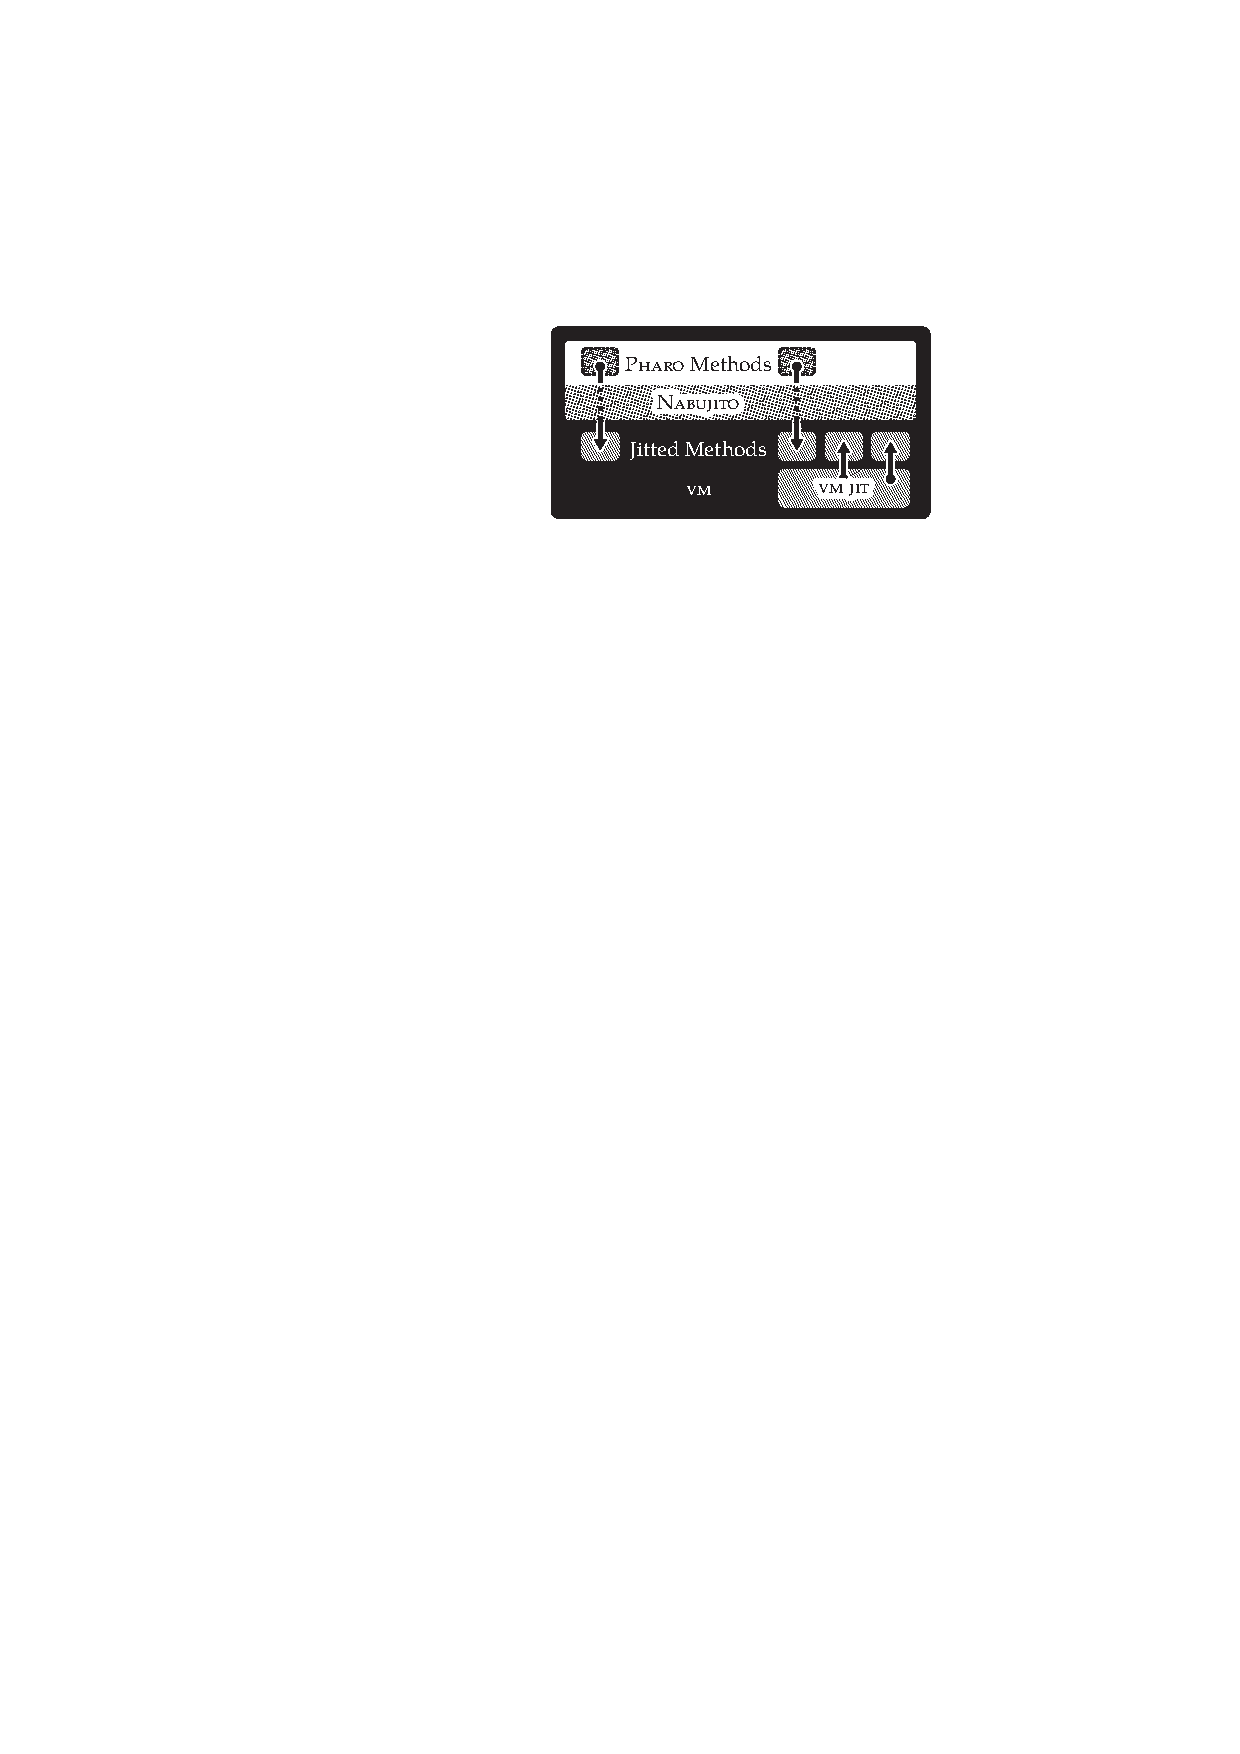
\includegraphics[scale=\imagescale]{nabujito-overview}
\end{figure}

\noindent In this section we present \NBJ, a \B-based approach for a language-side \JIT compiler.
\todo{Introduction}

% ---------------------------------------------------------------------------
\subsection{Background}
\seclabel{val-nabujito-background}
% ---------------------------------------------------------------------------

\NBJ goes even further than \WF using almost the same techniques.
However, instead of focusing on primitives, \NBJ generates native executable code for standard \ST methods.
Primitives tend to be more low-level, whereas \NBJ focuses on high-level \ST code. 


%----------------------------------------------------------------------------
\paragraph{The \JIT of the \PH \VM}
The \PH \VM (Cog) already comes with a \JIT that translates bytecodes to native instructions.
It transforms \ST methods into slightly optimized native code at runtime.
The main speed improvement comes from avoiding bytecode dispatching and by inlining certain known operations and primitives \cite{Ayco03a}.
The most complex logic of the \JIT infrastructure deals with the dynamic nature of the \ST environment.
Methods and classes can be changed at runtime and that has to be addressed by the \JIT infrastructure.
The \JIT compiler, by which we refer in this context to the transformation of bytecodes to native code, represents a small part of the whole infrastructure.
There exists more important stages as an additional register allocation pass to reduce the number of stack operations \cite{Mira99a,Mira11a}.
The existing \JIT infrastructure is implemented in \Slang \cite[Ch.\ 5]{Blac09a} as the rest of the \VM.

To understand the upcoming implementation issues of \NBJ we have to dive into the details of \PH's \JIT.
\PH uses a flavor of the \Cog \VM which evolved in several steps from a simple bytecode interpreter.
A successful and fast \JIT implies a \VM that uses the native stack.

The original \ST-80 blue book implementation foresees a spa\-ghet\-ti-stack where all contexts are normal objects on the heap.
This design simplifies the \VM implementation significantly since there is no special treatment necessary for blocks.
Also this makes it rather easy to implement \PH's feature to access the current context using the special \ttt{thisContext} variable.
However, the obvious down side of this implementation is the massive stress on the \GC.
For each message send a new context has to be allocated and on each return contexts have to be reclaimed.
It would naturally be more efficient to use the native stack which allows for cheap allocation and precise reclaiming of method context.
While this mapping can be done rather easily there are three properties of \PH that make this hard: blocks, non-local returns and the mentioned \ttt{thisContext}.
Eliot Miranda eventually succeeded to implement an efficient mapping scheme for the \Cog \VM that is based on the original work done by Peter Deutsch and Allan Schiffman \cite{Deut84a}.

Even so the basic concepts of the native stack mapping are easy to understand the final implementation is tricky details.
Real closures that outlive their outer method activation context make the mapping difficult.
At the same time all the reflective capabilities to modified the stack from within \PH have to be supported.
This, in return limits the optimization opportunities.
\Cog chose a path in between where most reflective modifications of the stack are permitted.
However, in certain exotic edge cases the \VM does not support the operation.

After supporting the native stack the next optimization in line is the real \JIT infrastructure where the \VM generates native code on the fly.
In \Cog there is a bytecode compiler that generates a simple intermediate representation which then is used to generate the final native instructions.
The \IR makes it easier to support new platforms next to the default 32-bit x86 implementation.
\Cog applies minor optimizations like a simple register allocation strategy to lower the stress on stack usage.
The most underestimated optimization is the fact that all the native code for the jitted methods is stored in a compact separate memory region.
This lowers the chances of cache misses, an ever growing problem on modern \CPU architectures.

\figref{cog-memory} gives and overview of the memory separation used by \Cog.
%
\begin{figure}[h]
	\centering
	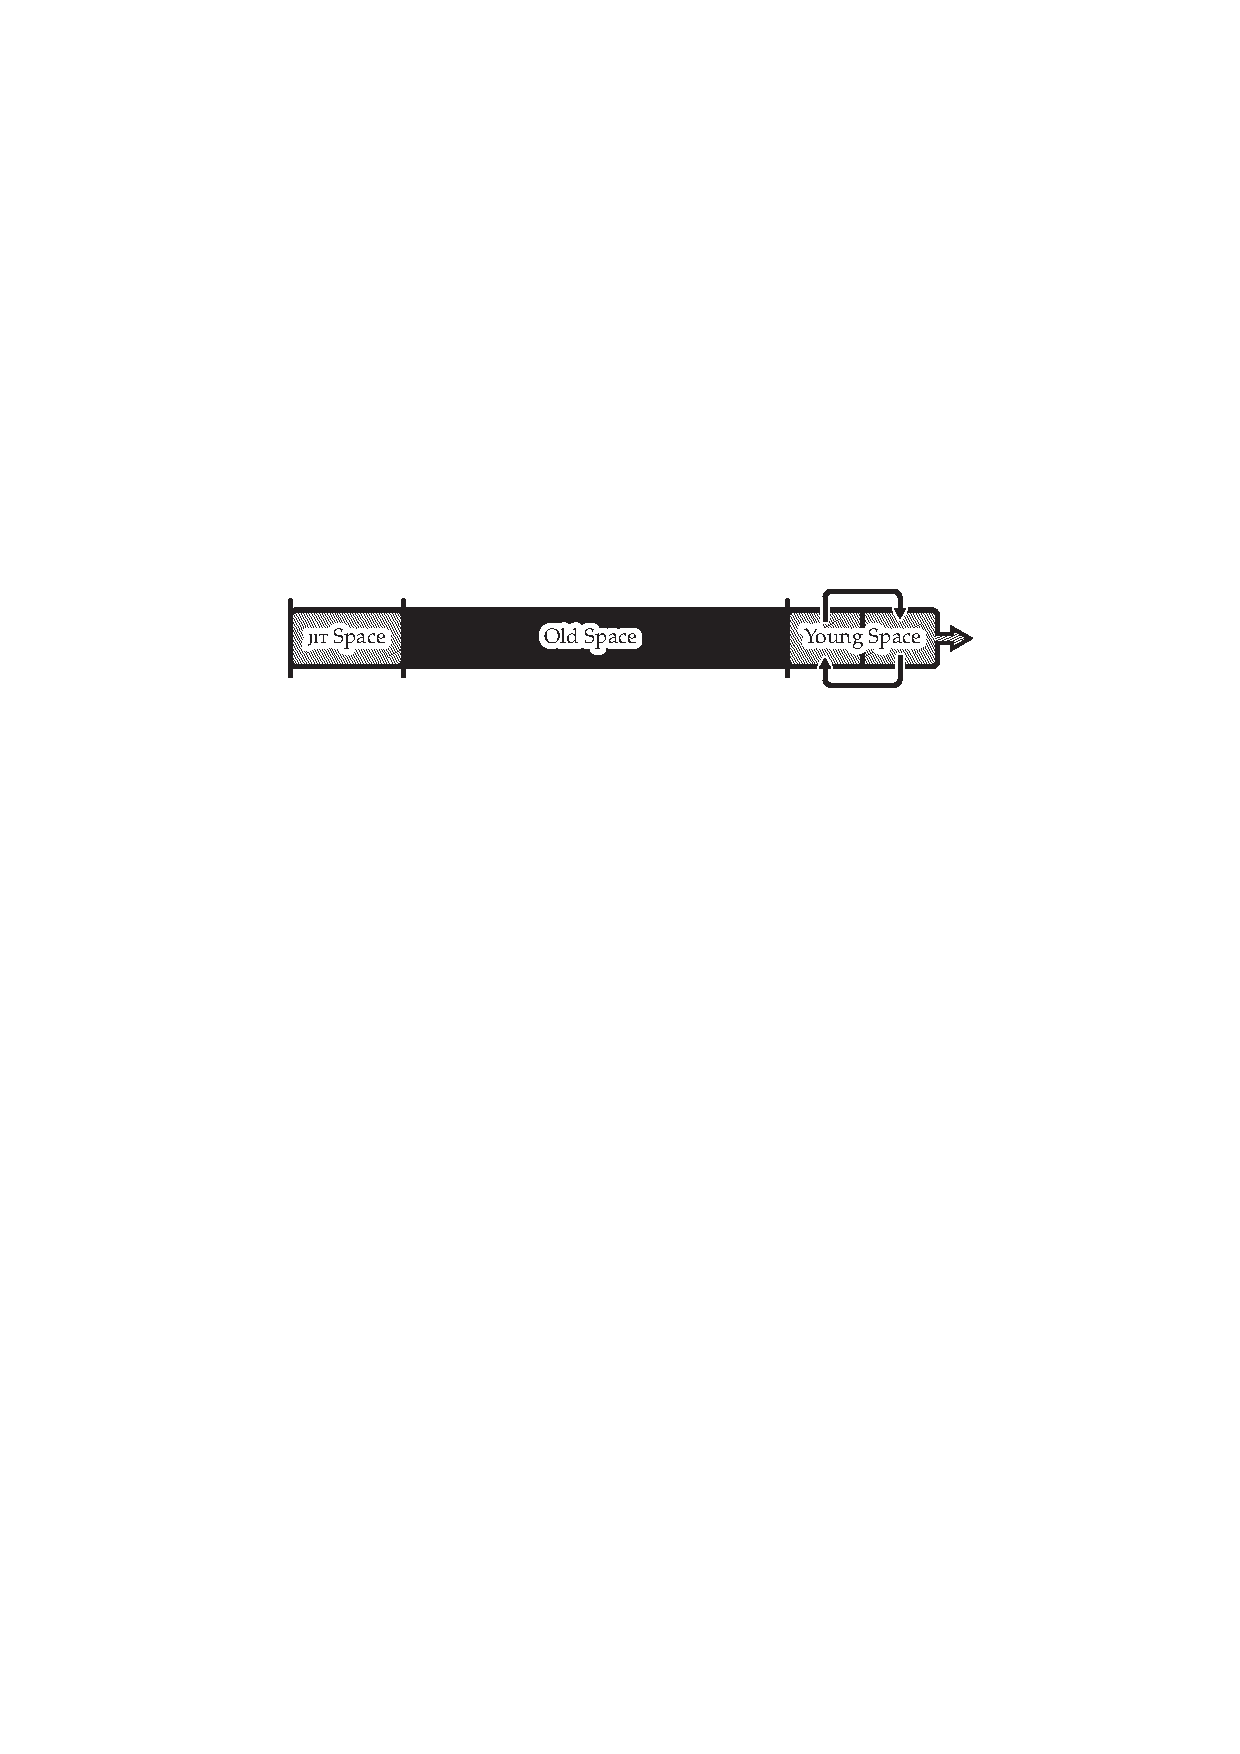
\includegraphics[scale=\imagescale]{cog-memory}
	\caption[\Cog Memory Model Overview]{\Cog Memory Model Overview: Fixed-sized \JIT space, slow changing old space and fast young space.}
	\figlabel{cog-memory}
\end{figure}
%
New objects are allocated in the young space which uses a fast semispace \GC with frequent reclaiming.
Objects that survive a \GC pass move to the old space where infrequent reclaims happen.
Separated from the two memory regions where normal \PH objects reside is the \JIT space dedicated for native code.
In \Cog the \JIT space has its own \GC strategy tailored to native code which is stored in a structure called \CogMethod.
Each jitted \PH method has a corresponding \CogMethod with native code which resides in the \JIT space.
The \CogMethod caches certain information such as the selector or number of arguments.
Again this improves code locality as all the frequently accessed information resides in the \JIT space.
\figref{cog-method} gives an overview of the \CogMethod.
We see that additionally to the cached meta information there is relocation information (method map) attached to the \CogMethod.
This is used to update object reference, typically to selectors, form the native code in sync with the objects that were moved in a \GC pass.
The same information is also used to update jumps to other native code in the \JIT space if the dedicated \JIT \GC performs a compaction.
%
\begin{figure}[h]
	\centering
	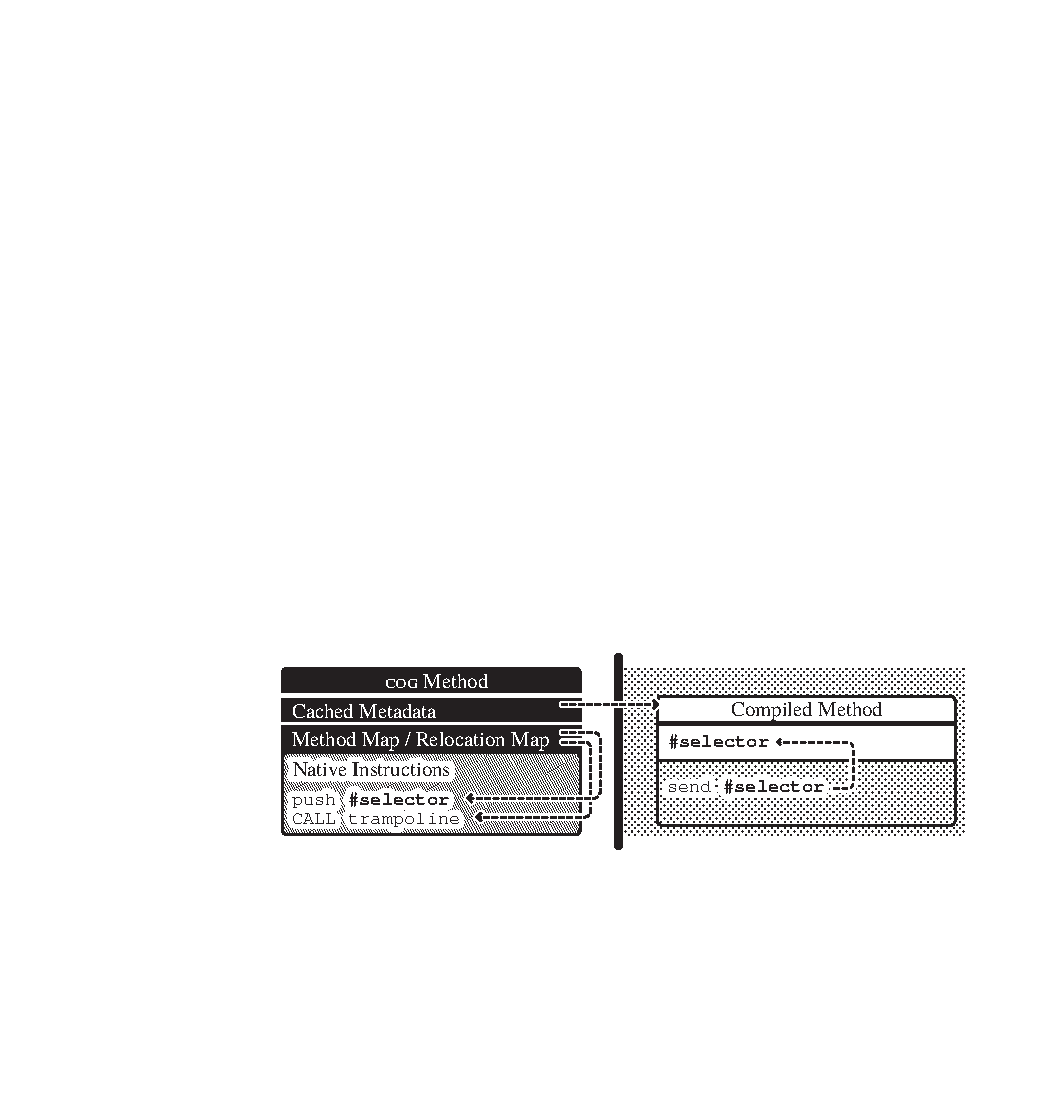
\includegraphics[scale=\imagescale]{cog-method}
	\caption[\Cog Method]{\Cog Method: Compiled method representation at \JIT-level residing in the \JIT memory space.}
	\figlabel{cog-method}
\end{figure}

\noindent So far we explained how \Cog uses native stack mapping for performance reasons and how the basic \JIT compiler works.
The limit the stress on the \CPU cache only the most used methods are jitted.
\Cog uses a hierarchy of inline caches to avoid the costly method lookup and checks if a method is already jitted or not.
Message sends from one jitted method to another hence happen with a very low overhead.
However, due to the limited size of the \JIT space that still means that infrequently used methods are evaluated using the existing bytecode interpreter.
\cb{the previous paragraph might be a bit dense, depending on the knowledge of the reader}



\todo{Step 3: Trampolines to jump back and forth between native activated scheme and bytecode interpreter based approach}\\

%----------------------------------------------------------------------------
\paragraph{Limitations of \VM-level \JIT Compilers}
In the context of \NBJ we separate a \JIT infrastructure into separate parts.
The major part is to have a \VM that uses stack-mapping.
In the case of a bytecode-based interpreter, we assume that the \VM provides routines to switch between a bytecode interpretation context and a low-level native execution context.
With \NBJ we move the \JIT compiler,the part that generates native code at runtime, from the \VM to the image.%, the part that generates native code at runtime, typically from bytecodes.
 Since the \JIT compiler is quite decoupled from the rest of the \JIT infrastructure we believe that a hard-coded static and low-level implementation is not optimal for several reasons:

\begin{itemize}
	\item Optimizing \ST code requires strong interactions with the dynamic environment.
	\item Accessing language-side properties from the \VM-side is hard.
	\item Changing the \JIT compiler requires changes at \VM-level.
	\item The \JIT reimplements primitives for optimization reasons resulting in code duplication.
\end{itemize}

\paragraph{Optimization Limitations for \PH}
In \ST methods tend to be very small and it is considered good practice to delegate behavior to other objects.
This implies that several common optimization techniques for static languages do not work well.
Dynamic method activation does not provide enough context for a static compiler to optimize methods.
Hence after inline caches and register allocation the next optimization technique is inlining.
However, inlining in a dynamic context is difficult and requires hooks at \VM-level to invalidate native code when the language-side changes.
Since in \PH, compiling a method to bytecode is handled completely with language-side code most of the infrastructure to get notified about method changes is already present.

\paragraph{Primitives in the Existing \JIT}
The existing \JIT reimplements the most used primitives at \VM-level.
This guarantees that the \VM stays as long as possible in the \JIT context (see \secref{benzo-jit-interaction} on page~\pageref{sec:benzo-jit-interaction}).
Additionally this enables new performance optimizations that for instance are hard to achieve with standard compliant C code.
A typical example is the integer addition which has to deal with overflow checks and conversion of tagged integers.
In \secref{val-waterfall} we describe how \WF suffers a similar constraint.
\WF manually defines such primitives in terms of native assembler instructions through the language-side \B interface.
\NBJ reuses the same optimized primitives so we rely on a single optimized definition which is shared among all native code libraries.

%----------------------------------------------------------------------------
\subsection{\NBJ Implementation}
\seclabel{val-nabujito-implementation}
%----------------------------------------------------------------------------
\NBJ is an experimental \JIT implementation which replaces the bytecode to native code translation of the existing \JIT infrastructure with a dynamic language-side implementation.
\NBJ is implemented mainly with a visitor strategy over the existing intermediate bytecode representation. 
Additionally we reimplemented vital native routines for the \JIT which are not directly exported by the \VM using \B. 
\cb{not sure if better to put down next to the \JIT limitation paragraphs...}
Nabujito relies on the following \VM-level infrastructure to manage and run native code for any \PH method:

\begin{itemize}[noitemsep,nolistsep]
	\item native stack management,
	\item routines for switching contexts,
	\item \JIT-level memory management for code segments.
\end{itemize}

\noindent The native stack mapping is an implicit requirement for an efficient \JIT.
Since this feature requires deep changes at \VM-level we can not alter or reimplement this at language-side.
However, the routines for switching between \JIT and non-\JIT execution context can be mostly reimplemented at language-side.
We only chose to implement a small subset of them with \B that were directly required for performing message sends.
Some of the helper routines' C-level addresses are easily accessible from language-side using \ttt{dlsym}.
Hence we reuse these for simplicity and only reimplemented the ones that are "hidden".
The last item we reuse, \JIT-level memory management, poses certain problems as we have little to no control over this from language-side.
There is no well-defined interface to interact with the \JIT from language-side in \PH.
However, to properly interact with the \JIT we have to tell it where references to language-side objects are located in the native code.
To overcome this limitation we chose to hack the current \VM to better interact with the \JIT.
More details on this topic follow in the following paragraphs.

\paragraph{\NBJ Dynamic Code Generation}
\NB mainly consists of a visitor over the bytecode-level \IR that is provided by the \PH compiler.
Additionally we reimplemented some of the aforementioned helper routines to switch execution context in the \VM.
The main difficulty of the \NBJ compiler is the missing interface to the \JIT.
For instance we did not have direct control on which methods in \PH are jitted or not, or to force-\JIT a method.
We added one additional primitive to be able to manually trigger \JIT compilation.

For standard methods \NBJ takes the bytecodes and transforms them with a visitor to native code.
It also applies simple optimizations such as creating low-level branches for \PH-level branching operations such as \ttt{ifTrue:}.
Optimizations for additional methods are all implemented flexibly at language-side.
Wherever possible, we reimplement the same behavior as the existing native \JIT compiler.

Eventually the native code is ready and \B attaches it to the existing compiled method.
At this point we benefit from the \JIT integration of \B itself.
As a reminder, we have shown in \secref{benzo-benzo} how \B-enabled methods are treated like normal primitive methods.
The \VM triggers a \B primitive which itself then jumps to the native code attached to the \B-enabled method.
By default the \Cog \JIT can only directly inline the native code for a known set of primitives.
As we have shown in \secref{benzo-jit-interaction} that the \Cog's \JIT was made aware of the special behavior of the \B primitive.
Hence, whenever a \B-enabled method is jitted its native code is directly accessible to the \JIT and inlined.
Thus we essentially remove the overhead of activating \B-enabled methods since we do not have to leave the \JIT execution mode.
As a result we call \B-enabled methods at the same speed as the existing \JIT.


\paragraph{Talking to the \JIT}
After the initial promising progress on building \NBJ on top of \B we soon realized that is does not suffice to just generate the equivalent native code as the \VM internal \JIT.
The first goal was to compile a simple method that just returns a constant integer.
Even at this stage it became apparent that there is a missing interface to the \JIT.
To explain that we have a look at the standard stack frame setup of a jitted method in \Cog shown in \lstref{val-nabujito-cog-frame}.
%
\begin{numstcode}[
	caption={\Cog \JIT Stackframe Setup},
	label={lst:val-nabujito-cog-frame}]{7}
push EBP
mov  EBP, ESP
push 0x1f452b00<CogMethod>
mov  EBX, 0x1f500004<nil>
push EBX
push EBX
\end{numstcode} 
%
After finishing executing these setup instructions the stack frame looks as depicted in \figref{val-nabujito-cog-stack-frame}.
%
\begin{figure}[h]
	\centering
	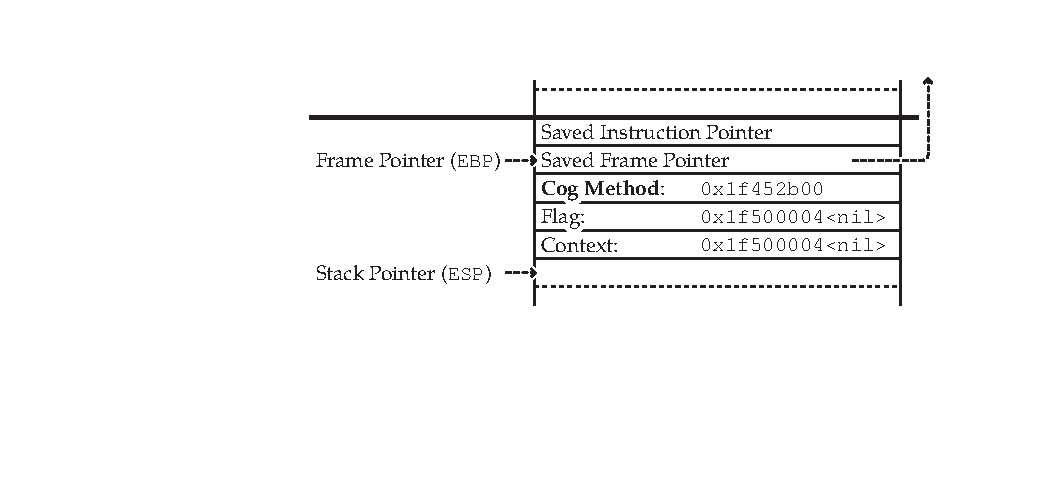
\includegraphics[scale=\imagescale]{cog-stack-frame}
	\caption{\Cog Stack Frame Header}
	\figlabel{val-nabujito-cog-stack-frame}
\end{figure}
%
As we can see there are already two references to \ttt{nil} in the stack frame header.
Already these two references pose a problem in a simple \NBJ setup, but for now we focus on the reference to the \CogMethod.
As we explained earlier the \CogMethod is a meta object at \JIT-level to make certain information of \PH methods faster accessible.
The \VM currently keeps a pointer to the class, the selector or the number of arguments cached in there.
Having the information there improves locality and make the assembler code required for the frequent querying simpler.
Going back to the native code in \lstref{val-nabujito-cog-frame} we see that we need the final address of the \CogMethod for the frame setup.
However, at the moment where \NBJ generates the native code the target method is not yet jitted.
This again implies that the corresponding \CogMethod has not yet been allocated by the \JIT.
And since the native code has to be installed in the \JIT we inevitably have to wait for \NBJ to finish compilation, we are stuck.

Instead of directly putting the absolute address of the meta-object in the native code we add a call to a helper routine which will patch the original code on the first activation.
We can do so since we know the following things:
\begin{itemize}[noitemsep,nolistsep]
	\item \CogMethod has a fixed size known upfront,
	\item we know the relative offset of the jitted method's instruction to the start of its \CogMethod,
	\item we can access the instruction pointer with a helper routine.
\end{itemize}
%
\noindent With this information we modify \NBJ to generate the modified frame setup show in \lstref{val-nabujito-frame-setup}.
%
\begin{numstcode}[
	caption={\NBJ Stack Frame Setup},
	label={lst:val-nabujito-frame-setup}]{7}
push EBP
mov  EBP, ESP

mov  EAX, 0x643d02e<pushCogMethodHelper>
call EAX
\end{numstcode}
%
In the \ttt{pushCogMethodHelper} we access the instruction pointer from where the call happened in the stack frame setup and deduce the start of the \CogMethod.
Once the address of the \CogMethod is retrieved the \ttt{pushCogMethodHelper} patches the \ttt{MOV} and \ttt{CALL} instruction in the jitted method.
The result is shown in \lstref{val-nabujito-patched-frame-setup}.
%
\begin{numstcode}[
	caption={\NBJ Patched Stack Frame Setup},
	label={lst:val-nabujito-patched-frame-setup}]{7}
push EBP
mov  EBP, ESP

push 0x1f452b00<CogMethod>
nop
\end{numstcode}
%
By using this indirection we circumvent the missing interface to the \JIT.
The helper routine only imposes a one-time overhead, however we slow down the final execution of the \NBJ method by a single \ttt{NOP} instruction.
Yet, looking at the \Cog stack frame in \figref{val-nabujito-cog-stack-frame} we only dealt with finding the reference to the \CogMethod.
So far we left out the \GC interaction at \JIT-level, which leads us to the following paragraph.

\paragraph{Overcoming the \GC Missing \VM Interface for the \JIT}
\Cog embeds references to normal \PH objects in its jitted methods.
Most often this is the case for the symbols used as selectors in message sends.
This is different from the indirection approach used in compiled methods for the bytecode interpreter.
There all objects used in the method are stored in a separate literal array and referenced by an index.
Hence the bytecode can stay very compact and more importantly does not have to be updated on each \GC pass.
While for space consumption was the only concern on the early \ST implementation the only thing the \JIT focuses on is performance and thus avoiding as many indirections possible.

\todo{explain the proplem of object relocation vs. native code}

% -----------------------------------------------------------------------------
\subsection{\NBJ Validation}
\seclabel{val-nabujito-performance}
% -----------------------------------------------------------------------------

\todo{missing intro}

% -----------------------------------------------------------------------------
\subsubsection*{Compilation Time}


The performance evaluation for our \B-based \JIT compiler is focused on the language-side code-generation part.
\NBJ essentially generates the same native code as the \VM-level \JIT, hence there is no performance difference at evaluation time.
However, \NBJ is clearly slower during the warm-up phase.
Compilation of the native instructions will take considerably more time compared to the \VM-level implementation of the same bytecode to assembler transformation.
The cost of transforming the bytecodes to native code at \VM-level can be measured in native instructions, whereas the unit at language-side is bytecodes.
However, we point out again, that this is a one-time overhead.
From the in-production experience of \NB, the \B-based \FFI (see \secref{ffi-evaluation}), we know that these costs amortized, especially for long-term applications.
Instead of focusing on the final performance of the generated code, we present the compilation time compared to the normal \PH bytecode compiler, which also resides at language-side.

\begin{table}[!ht]
    \centering
    \begin{tabular}{rS}
                      & {Compilation Time [ms]} \\\midrule
        \PH Compiler  & 71(1) \\
        \NBJ          & 73(1)
    \end{tabular}
    \caption[\NBJ Compilation Speed]{Compilation efforts of the standard \ST compiler in \PH and \NBJ for the a simple method returning the constant \ttt{nil}.}
    \tablabel{val-nabujito-performance-small}
\end{table}

\noindent In \tabref{val-nabujito-performance-small} we compare the compilation speed of the standard \PH compiler and \NBJ.
We measure the accumulated time spent to compile the method 1000 times.
The average and deviation are taken over 100 runs. 
The \PH compiler takes source code as input and outputs \ST bytecodes.
\NBJ takes bytecodes as input and outputs native code.

We see that in the simple case displayed in \tabref{val-nabujito-performance-small} \NBJ's compilation speed lies within the same range as the standard \ST compiler.
We expect that in the future we apply more low-level optimizations and thus increase the compilation time of \NBJ.
However, we have shown in the performance evaluation for \NB, the \B-based \FFI, in \secref{ffi-evaluation} that even a rather high one-time overhead is quickly amortized.
Furthermore with \ST's image approach the generated native code is persistent over several sessions.
A subsequent restart of the same runtime will not cause the \JIT to nativize the same methods it did during the last launch.
Hence our approach is even valid for short-timed script-like applications as most of the methods will already be available in optimized native code from a previous run.

% -----------------------------------------------------------------------------
\subsubsection*{Per Method Comparison}
\todo{choose simple enough methods that we can compile with nabujito: currently only + works}


% -----------------------------------------------------------------------------
\subsection{Problems}
\seclabel{val-nabujito-problems}
% -----------------------------------------------------------------------------
\paragraph{Hidden \VM Internals}
\todo{backref to patch methods}\\
\todo{maintenance problem: \NBJ harcodes the \VM interaction} \\
\todo{unsuited \VM architecture for a feasible real-world \JIT} \\
\todo{focusing on a future version on SISTA}


\paragraph{Debugging Cycle}
\todo{Missing tools to directly interact with benzo / the real vm} \\
\todo{missing small assembler tests} \\
\todo{reactivate the VM simulator infrastructure} \\
\todo{missing \VM development tools under \PH (mainly disassembler)}

\paragraph{Missing Optimizations}
One major performance optimization missing in both, the original \PH \VM-level \JIT and \NBJ, is inlining. 
By inlining we are able to create methods that are potentially big enough for optimizations.
However, inlining is a difficult task in a highly dynamic language such as \ST or \Self \cite{Cham89a}. 
Efficient inlining can only be performed with sufficient knowledge of the system. 
Accessing this high-level information from within the \VM is cumbersome and requires duplication of language-side reflective features.
The \JIT lives on the same level as the information it needs relying on the already present reflective features of \ST.


% ===========================================================================
\section{Outlook}
% ===========================================================================

\todo{Common problem: missing debugging infrastructure} \\
\todo{\WF and \NBJ share the same problems} \\
\todo{For speed a proper \JIT interface is missing } \\
\todo{SISTA} \\
\todo{better intermediate format (VCPU) from \B}

% ===========================================================================
\section{Summary}
% ===========================================================================


% =============================================================================
\ifx\wholebook\relax\else
    \end{document}
\fi
\documentclass[a4paper,12pt,twoside]{../includes/ThesisStyle}
\usepackage[utf8]{inputenc}
\usepackage[T1]{fontenc}

\usepackage[left=1.5in,right=1.3in,top=1.1in,bottom=1.1in,includefoot,includehead,headheight=13.6pt]{geometry}\renewcommand{\baselinestretch}{1.05}


% =============================================================================
%\usepackage[sectionbib]{chapterbib}	% Cross-reference package (Natural BiB)
%\usepackage{bibunits}
%\usepackage{natbib}					% Put References at the end of each chapter
\usepackage{algorithm}
\usepackage{alltt}
\usepackage{amsfonts}
\usepackage{amsmath}
\usepackage{amssymb}
\usepackage{cite}
\usepackage{color}
\usepackage{enumerate}
\usepackage{booktabs} % used for \midrule
\usepackage{fancyhdr}					% Fancy Header and Footer
\usepackage{graphicx}
\usepackage{ifthen}
\usepackage{latexsym}
\usepackage{multirow}
\usepackage{rotating}					% Sideways of figures & tables
\usepackage{stmaryrd}
\usepackage{subfigure}
\usepackage{url}         
\usepackage{xspace}
\usepackage[normalem]{ulem} % for \sout
\usepackage{xcolor}
\usepackage{tablefootnote}
\usepackage{pifont}

% =============================================================================

% Table of contents for each chapter
\usepackage[nottoc, notlof, notlot]{tocbibind}
\usepackage{minitoc}
\setcounter{minitocdepth}{1}
\mtcindent=15pt

\setcounter{secnumdepth}{3}
\setcounter{tocdepth}{2}
  
% =============================================================================
% Fancy Header Style Options

\pagestyle{fancy}                       % Sets fancy header and footer
\fancyfoot{}                            % Delete current footer settings

%\renewcommand{\chaptermark}[1]{         % Lower Case Chapter marker style
%  \markboth{\chaptername\ \thechapter.\ #1}}{}} %

%\renewcommand{\sectionmark}[1]{         % Lower case Section marker style
%  \markright{\thesection.\ #1}}         %

\fancyhead[LE,RO]{\bfseries\thepage}    % Page number (boldface) in left on even
% pages and right on odd pages
\fancyhead[RE]{\bfseries\nouppercase{\leftmark}}      % Chapter in the right on even pages
\fancyhead[LO]{\bfseries\nouppercase{\rightmark}}     % Section in the left on odd pages

\let\headruleORIG\headrule
\renewcommand{\headrule}{\color{black} \headruleORIG}
\renewcommand{\headrulewidth}{1.0pt}
\usepackage{colortbl}
\arrayrulecolor{black}

\fancypagestyle{plain}{
  \fancyhead{}
  \fancyfoot{}
  \renewcommand{\headrulewidth}{0pt}
}


% =============================================================================
% Clear Header Style on the Last Empty Odd pages
\makeatletter

\def\cleardoublepage{\clearpage\if@twoside \ifodd\c@page\else%
  \hbox{}%
  \thispagestyle{empty}%              % Empty header styles
  \newpage%
  \if@twocolumn\hbox{}\newpage\fi\fi\fi}

\makeatother

\newenvironment{maxime}[1]
{
\vspace*{0cm}
\hfill
\begin{minipage}{0.5\textwidth}%
%\rule[0.5ex]{\textwidth}{0.1mm}\\%
\hrulefill $\:$ {\bf #1}\\
%\vspace*{-0.25cm}
\it 
}%
{%

\hrulefill
\vspace*{0.5cm}%
\end{minipage}
}

\let\minitocORIG\minitoc
\renewcommand{\minitoc}{\minitocORIG \vspace{1.5em}}


\renewcommand{\epsilon}{\varepsilon}

% centered page environment
\newenvironment{vcenterpage}
	{\newpage\vspace*{\fill}\thispagestyle{empty}\renewcommand{\headrulewidth}{0pt}}
	{\vspace*{\fill}}
	

%=============================================================================

\usepackage{needspace}
\newcommand{\needlines}[1]{\Needspace{#1\baselineskip}}

\usepackage{xcolor}
\definecolor{source}{gray}{0.95}
% source code formatting
\usepackage{listings}
    % global settings for source code listing package
\lstset{
    basicstyle=\ttfamily\small,
    showspaces=false,
    showstringspaces=false,
    captionpos=b, 
    columns=fullflexible}

\lstdefinelanguage{ST}{
    keywordsprefix=\#,
    morekeywords=[0]{true,false,nil},
    morekeywords=[1]{self,super,thisContext},
    morekeywords=[2]{ifTrue:,ifFalse:,whileTrue:,whileFalse:,and:,or:,xor:,not:,by:,timesRepeat:},
    sensitive=true,
    morecomment=[s]{"}{"},
    morestring=[d]',
    escapechar={!},
    alsoletter={., :, -, =, +, <},
    moredelim=**[is][\itshape]{/+}{+/},
    literate=
        {^}{{$\uparrow$}}1
        {:=}{{$\leftarrow$}}1
        {~}{{$\sim$}}1
        {-}{{\sf -\hspace{-0.13em}-}}1  % the goal is to make - the same width as +
        {+}{\raisebox{0.08ex}{+}}1		% and to raise + off the baseline to match V
        , % Don't forget the comma at the end!
    style=STStyle
}
\lstdefinestyle{STStyle}{
    tabsize=4,
    %frame=leftline,
    % frame=bl,
    %framerule=2pt,
    %rulecolor=\color{gray},
    % backgroundcolor=\color{white},
    %backgroundcolor=\usebeamercolor[bg]{listing},
    basicstyle=\ttfamily\small,
    keywordstyle=\bf\ttfamily,
    % stringstyle=\color{orange},
    stringstyle=\mdseries\slshape,
    commentstyle=\it\rmfamily\color{darkgray}, 
    commentstyle=\mdseries\slshape\color{gray},
    %commentstyle=\mdseries\slshape,
    emphstyle=\bf\ttfamily,
    escapeinside={!}{!},
	%backgroundcolor=\color{source},
    %emphstyle={[2]\color{red}},
    %emphstyle={[3]\color{blue}\bf},
    %emphstyle={[4]\color{blue}},
    keepspaces=true
} 

%\lstnewenvironment{javacode}  [1][]{\lstset{language=java,#1}\needlines{#2}}{} 
%\lstnewenvironment{pythoncode}[2][]{\lstset{language=python,#1}\needlines{#2}}{}
\lstnewenvironment{stcode}    [2][]{\lstset{language=ST,#1}\needlines{#2}}{}
\lstnewenvironment{ccode}     [2][]
    {\lstset{language=C,numbers=left,escapechar=\$,numberstyle=\tiny,#1}\needlines{#2}}{}

% ON: I tried to pass the line number options in as arg #1 but it does not work for me
% I also could net get the line numbers to consistently increase
\lstnewenvironment{numstcode} [2][]
    {\lstset{language=ST,numbers=left,numberstyle=\tiny,numbersep=2pt,#1}\needlines{#2}}{}
\lstnewenvironment{numstcodecont} [2][]
    {\lstset{language=ST,numbers=left,numberstyle=\tiny,numbersep=2pt,firstnumber=last#1}\needlines{#2}}{}

\newcommand{\lst}[1]{{\tt #1}}

% In-line code (literal)

% In-line code (latex enabled)
% Use this only in special situations where \ct does not work
% (within Section headings ...):
\newcommand{\lct}[1]{{\textsf{\textup{#1}}}}
% Code environments
\lstnewenvironment{code}{%
	\lstset{%
		% frame=lines,
		frame=single,
		framerule=0pt,
		mathescape=false
	}
}{}

%\renewcommand{\lstlistingname}{Code Example}

% =============================================================================
\newboolean{showcomments}
\setboolean{showcomments}{true}

\ifthenelse{\boolean{showcomments}} {
	\newcommand{\ugh}[1] {\textcolor{red}{\uwave{#1}}}	% please rephrase
	\newcommand{\ins}[1] {\textcolor{blue}{\uline{#1}}}	% please insert
	\newcommand{\del}[1] {\textcolor{red}{\sout{#1}}}	% please delete
	\newcommand{\chg}[2] {								% please change
		\textcolor{red}{\sout{#1}}{\ra}
		\textcolor{blue}{\uline{#2}}}
	\newcommand{\nbc}[3]{								% comment
		{\colorbox{#3}{\bfseries\sffamily\scriptsize\textcolor{white}{#1}}}
		{\textcolor{#3}{\sf\small$\blacktriangleright$\textit{#2}$\blacktriangleleft$}}}

}{
	\newcommand{\ugh}[1]{#1}							% please rephrase
	\newcommand{\ins}[1]{#1}							% please insert
	\newcommand{\del}[1]{}								% please delete
	\newcommand{\chg}[2]{#2}							% please change
	\newcommand{\nbc}[3]{}								% comment
}

% =============================================================================
\usepackage[pagebackref,hyperindex=true]{hyperref}


% Links in pdf
\usepackage{color}
\definecolor{linkcol}{rgb}{0.0, 0.0, 0.0} 
\definecolor{citecol}{rgb}{0.0, 0.0, 0.0} 

% Change this to change the informations included in the pdf file
% See hyperref documentation for information on those parameters
\hypersetup {
	bookmarksopen=true,
	pdftitle="Design and Use of Anatomical Atlases for Radiotherapy",
	pdfauthor="Olivier COMMOWICK", 
	pdfsubject="Creation of atlases and atlas based segmentation", %subject of the document
	%pdftoolbar=false, % toolbar hidden
	pdfmenubar=true, %menubar shown
	pdfhighlight=/O, %effect of clicking on a link
	colorlinks=true,
	pdfpagemode=UseNone,
	pdfpagelayout=SinglePage,
	pdffitwindow=true,
	linkcolor=linkcol,
	citecolor=citecol,
	urlcolor=linkcol
}

% =============================================================================
\newcommand{\figlabel}[1] {\label{fig:#1}}
\newcommand{\chaplabel}[1]{\label{chap:#1}}
\newcommand{\seclabel}[1] {\label{sec:#1}}
\newcommand{\tablabel}[1] {\label{tab:#1}}
\newcommand{\lstlabel}[1] {\label{lst:#1}}

\newcommand{\figref}[1] {Figure~\ref{fig:#1}}
\newcommand{\chapref}[1]{Chapter~\ref{sec:#1}}
\newcommand{\secref}[1] {Section~\ref{sec:#1}}
\newcommand{\tabref}[1] {Table~\ref{tab:#1}}
\newcommand{\lstref}[1] {Listing~\ref{tab:#1}}

\newcommand{\commented}[1]{}

\newcommand{\bs}    {\symbol{'134}} % backslash
\newcommand{\us}    {\symbol{'137}} % underscore
\newcommand{\ttt}[1]{\texttt{#1}}
\newcommand{\ie}    {\emph{i.e.},\xspace}
\newcommand{\eg}    {\emph{e.g.},\xspace}
\newcommand{\etal}  {\emph{et al.}\xspace}
\newcommand{\ns}    {\!\!\!\!} %big negative space
\newcommand{\cnull} {\textbackslash0\xspace}


\newcommand\fix[1]{\nb{FIX}{#1}}
\newcommand\todo[1]{\nb{TO DO}{#1}}
\newcommand\cb[1]{\nbc{CB}{#1}{purple}}
\newcommand\sd[1]{\nbc{SD}{#1}{orange}}
\newcommand\is[1]{\nbc{IS}{#1}{gray}}
\newcommand\gc[1]{\nbc{GC}{#1}{olive}}
\newcommand\ct[1]{\nbc{CT}{#1}{teal}}
\newcommand\md[1]{\nbc{MD}{#1}{blue}}
\newcommand\dc[1]{\nbc{DC}{#1}{green}}

% =============================================================================
\newcommand{\NBFFI}  {Native\-Boost-FFI\xspace}
\newcommand{\NB}  {Native\-Boost\xspace}
\newcommand{\B}   {Benzo\xspace}
\newcommand{\ST}  {Small\-talk\xspace}
\newcommand{\PH}  {Pharo\xspace}
\graphicspath{{.}{../figures/}}

\begin{document}
% =============================================================================
\chapter{Future Work}
\chaplabel{future}
\minitoc
% =============================================================================
\introduction
% =============================================================================

In \chapref{background} we gave an overview of different concepts of reflection focusing on the main distinction between language-side and \VM-side reflection.
While language-side reflection is very well described in research and rather wide-spread in dynamic languages, the \VM-side counterpart is not.
Compile-time reflection is the center of many popular \VM generation frameworks, but they usually exclude the dynamic reflection aspect of the final binary.
Nevertheless, it is always possible to introspect (structural reflection) the \VM at a very basic level.
Additionally, there are tools like \DTrace which provide a simple way to instrument a binary with little prior setup required.
Thus a limited form of intercession is possible on the binary executable themselves.
However, this still does not make the internal structural information of the \VM accessible that were available at compilation time.
And the restrictions are even more severe when it comes to \VM-level intercession.
It is foreseen for languages to dynamically influence the underlying \VM.

In the course of this thesis we presented tools that try to enter the field of \VM-level reflection -- all based on \B, a common framework to activate native code from language-side.

\WF's dynamic primitives are a first step towards modifying \VM behavior from language-side in a rather controlled way.
By bringing the metacircular \VM sources alive in \PH we connect the former static definition to the running artifact.
Modification happen not by injecting basic native instructions but at high-level by modifying and dynamically compiling primitives.

In contrast to \WF we developed \NBJ, a \JIT compiler prototype, that moves the original \VM component to the language-side.
While \NBJ is defined as language-side compiler using familiar coding patterns, its interaction with the \VM is not clean.
Unlike the plugins and primitives defined by \WF the \JIT generates native code that is heavily depending on the low-level and internal execution model of the \VM.
Unlike \WF \NBJ requires a modified \VM to add a basic interface for manually injecting \JIT code.

In this chapter we present possible solutions and an early prototype \VM that addresses the limitations we encountered while developing \NB, the \B-based \FFI, \WF and \NBJ.
We start by listing possible improvements for the language-side part of the \B infrastructure such as providing a well-defined high-level intermediate format.
This will lead to a description of required \VM-level improvements to make applications such as \WF or \NBJ feasible outside a research context.
\todo{recheck to be in sync with the chapter structure}

% =============================================================================
\section{Background and Related Work}
\seclabel{future-related-work}
\seclabel{future-background}
% =============================================================================
The improvements to the existing infrastructure \B and possible future work is influenced by two research projects we described already in detail in \secref{background-reified-vms}: the \P \VM and the \Klein \VM.
For this chapter we present a small summary of these two metacircular \VMs with the focus on two things: their own limitations compare to \B and their influence on improvements and future work.


% -----------------------------------------------------------------------------
\subsection{\P \VM}
% -----------------------------------------------------------------------------

The \P \VM \cite{Verw11a} presented in \secref{background-pinocchio} is a direct predecessor of the work presented in this thesis.
The knowledge gained while participating on \P had a great influence on the development direction of \B and its applications.

Unlike \PH running on the \Cog \VM the \P research \VM has no bytecode interpreter.
The only execution base is native code which is directly generated by the language-side compiler.
At the current stage of development \P has not yet support for a separate image as in \PH.
The runtime image is currently defined by the bootstrap process where classes, objects and methods are exported into binary images and linked together with a primitive kernel to a final executable.

\paragraph{Going Native}
We took from \P that language-side native code generation is not more complex than generating bytecodes.
Instead we directly embrace the native world.
This means that in the core \P already uses many concepts that are only introduced by the \JIT in the \Cog \VM.
Hence, \P does no longer distinct between \JIT mode and interpreter mode.
Here the gain for \P are twofold: we could boost the performance of the language-runtime and simplify the design by not needing a dual compilation pipeline for the \JIT and the bytecode.

\paragraph{Going Meta}
Even so \P directly uses native code as core execution mode we avoided to directly write native code if possible.
For instance the method lookup in \Cog is statically implemented at \VM-side using \Slang.
We described in \secref{background-pinocchio} in detail how \P uses language-side code instead for the lookup.
Using the combination of low-level code to flatten out meta recursion we still have full language-side control over the lookup while maintaining good performance.

\paragraph{Missing Low-level Reification}
The most obvious shortcoming of \P was the lack of its own garbage collector.
Instead of investing time into a separate well-defined \GC \P relies on the conservative \urlfootnote{Boehm \GC}{http://www.hpl.hp.com/personal/Hans_Boehm/gc/} built for C programs.
The Boehm \GC is sufficiently fast to run \P as a prototype, however, due to its generic nature it is not as efficient as a specific \GC.
However, \P lacked the necessary reification at level of the object layout to properly implement a \GC.
All the notion about the object layout in memory are hard-coded in the compiler in several places.

\paragraph{Missing C Independence:}
The second negative point of \P is its dependence from C.
During the course of the \P development we greatly reduced the quantity of C code.
However, for simplicity we relied on a small C Kernel for the complete bootstrap of the language.
Additionally some crucial primitives that required system calls were implemented in C.

% -----------------------------------------------------------------------------
\subsection{MIST: A C-less \ST Implementation}
% -----------------------------------------------------------------------------
\urlfootnote{\MIST}{http://mist-project.org/} is another prototype \ST \VM that follows similar goals as the \P \VM.
It not longer uses bytecode interpreter but only relies on native code.
However, it goes one step further than \P by not relying on any C-based infrastructure.
\MIST implements its own linker to build the final executable.
And unlike \P it does not require kernel primitives written in C.
\MIST brings its own implementation to directly perform system calls from within the language.


% -----------------------------------------------------------------------------
\subsection{\Maxine \VM}
% -----------------------------------------------------------------------------
\Maxine is a metacircular \Java \VM \cite{Wimm13a} focused on an efficient developer experience.
The \Maxine \VM stands out as it truly focuses on productivity and developer interaction.
\Maxine uses abstract and high-level representations of \VM-level concepts and consistently exposes them throughout the development process.
Inspectors at multiple abstraction levels are readily available while debugging, giving insights to the complete \VM state.
\Maxine provides and excellent navigation for generated native code by providing links back to language-side objects as well as other native code and symbols.

Compared to \Maxine, the \B infrastructure currently lacks the debugging tools which would enable a truly seamless interaction with the low-level world.
Namely, \B does not support low-level debugging and does not support facilities to inspect low-level native code directly.
However, \Maxine focuses on \Java, a language with inferior reflective capabilities compared to \PH.
Hence the live interaction with the \VM is only possible during the development phase and not exposed to the language-side.

% -----------------------------------------------------------------------------
\subsection{\Klein \VM}
% -----------------------------------------------------------------------------
\urlfootnote{\Klein}{http://kleinvm.sourceforge.net/} is a metacircular \VM for the \Self programming language that has no separation into \VM and language \cite{Unga05a}.
The \VM is entirely written in \Self but takes the concept of metacircular beyond the compile-time.
For instance, unlike many other metacircular \VMs, including \Cog and \Squeak, \Klein does not use an intermediate low-level language to bootstrap the system.
It generates directly a binary image, much like the aforementioned \P or \MIST \VM.
However, it is important to note that the \VM-level structures and objects are not compiled away as it is usually the case.
Instead the \VM structures are represented as real \Self objects.
Hence the \Klein \VM supports true \VM-level reflection since there is only a single code base.

Additionally to the advances in reflection and metacircularity, \Klein focuses on fast compilation turnarounds to allow for a responsive development process.
Which is unlike the \Squeak \VM where a full \VM bootstrap takes a order of minutes on modern hardware.
\Klein also supports advanced mirror-based debugging tools to inspect and modify a remote \VM.

Development on the \Klein \VM seized in 2009 and left the \Klein \VM in fairly usable state.
However, up to now it lacks a proper \GC which essentially limits its real-world application.
Yet, it proved that it is possible and build a language-runtime without a proper separation of the language-side and the \VM or base-level.
From the literature presented about the \Klein project we see a strong focus on the improvements of the development tools.
The fact that the language-runtime allows \VM-level reflection to change the \VM dynamically is not directly mentioned in the literature.
While we see the practical limitations of changing the \VM at runtime we would like to open the doors to this new form of reflection.

% =============================================================================


% =============================================================================
%\newpage
\section{Language-side Improvements}
\seclabel{future-language}
% =============================================================================
In this section we present the suggestion for improvements related mostly tied to the language-side part of \B.
Most of the solutions have been presented in the separate chapters of \B in \secref{benzo-problems}, \NB \FFI in \secref{ffi-problems} and the \B application prototypes (\secref{validation-waterfall-problems} and \secref{validation-nabujito-problems}).

% -----------------------------------------------------------------------------
\subsection{Improved Domain Specific Inspectors}
% -----------------------------------------------------------------------------
Domain specific inspectors are important for an efficient development as we pointed out in \secref{reification-inspectors}.
Similar to the \JIT approach we have to optimize the frequent tasks during development and provide a seamless integration.
This becomes even more important when working with low-level code and data that does not come with existing first-class structures.
We noticed that using \B for \NBJ and \WF that it is more convenient to rely on an existing low-level text-based debugger such as \ttt{gdb} to inspect C-level structures.

We have seen excellent use of inspectors in the \VM development of the \Cog \VM itself.
The original simulator supports inspecting objects in simulated raw memory.
\Cog added additional inspectors including disassembled instructions for the \JIT development.
However, with the recent changes the advanced simulator does not yet run in \PH and requires attention.

Lately we have seen a very similar approach for the \Maxine research \VM \cite{Wimm13a}.
It provides excellent low-level debugging interaction, switching seamlessly between low-level assembler views and high-level object inspectors.
We believe that it is an imperative requirement for a \VM development \IDE to support customizable inspectors that span from high-level to low-level.
Even though existing C-focused \IDEs provide more and more support for integrated inspectors the \VM domain has different needs.
C inspectors are tailored towards fixed-sized objects whose types can be statically inferred.
Whereas, for \VMs we only have a handful types of object layouts and the real type is only implicitly available.
For instance in certain \VMs the class is encoded in the header of an object instead of a simple full pointer to the class object.
This means that a minor interpretation pass is necessary to retrieve such information.
Which is why most C-focused \IDEs are only partially sufficient for an efficient \VM development.


% -----------------------------------------------------------------------------
\subsection{Virtual \CPU an Assembler \DSL}
% -----------------------------------------------------------------------------
\todo{relink}
\todo{read and weave in \cite{Lin12b} (ll DSL for high-level low-level programming)}\\
\B uses \AsmJIT as assembler backend which is currently limited to x86 instruction set.
This choice is aligned with \PH's main development focus for the most common operating systems.
However, this choice of architecture already excludes mobile devices which currently focus on \ARM-based architectures.
To support this new architecture we have to extend the assembler backend in \AsmJIT.
While the implementation effort for a new \AsmJIT architecture is an implicit requirement the implications on \B-based applications are more severe.
For instance we already mentioned in \secref{ffi-problems-platform} how the \NB \FFI would suffer from code duplication.
Essentially each newly added \CPU architecture has ripple-effects up to the final \B-based applications.
Each \B application has to duplicate all native usage in and create internally separate generates for each platform.
We believe that this approach is not the right path as it forces \B users into code duplication.

A much better solution is to provide a more abstract and platform independent low-level intermediate format at \B-level.
Ideally we can push the platform specific code generation fully to the native backends in \B itself.
\B-based applications only have to focus on a single low-level instruction format reducing the development effort.

We also noticed that for actual testing the native instruction set is not optimal.
For instance the x86 instruction with all its modifier codes and variable width instructions makes it tedious to implement a proper simulator.
Writing bindings for an existing simulator such as \urlfootnote{\Bochs}{http://bochs.sourceforge.net/} is a better choice.
However, even with a proper simulator ready for x86 we can not provide a very fluent debugging process.
For instance, the way assembler instructions are written in \B require them to be fully generated before they can be interpreted.
We are used from \PH that any code snipped is executable, a property that we would like to bring to the low-level development as well.

\paragraph{\VCPU: A Low-level Intermediate Format}
To reduce the aforementioned platform dependency of \B we developed a intermediate low-level representation called \VCPU.
It is based on a three-address-code (\TAC) to simplify the adoption of optimizations such as static single assignment (\SSA) \cite{Cytr91a}.
Additionally we chose to postpone register allocation to the final code generation phase.
By using a \TAC-based format and rewiring the internals we are even able to make the \VCPU code directly executable in \PH.

Before we go into the implementation details of \VCPU we show it is used.
\VCPU is based on \TAC instruction which take the following form:
%
\begin{stcode}{}
result := argument1 OP argument2
\end{stcode}
%
There are three operands involved, \ttt{result}, \ttt{argument1} and \ttt{argument2}, from which the name of this \TAC format originates.
Based on this assumption, each standard \VCPU instruction returns a temporary variable which can be used for further operations.
This makes the information-flow much more consistent.
For instance the x86 instructions which sometimes have a predefined result register and sometimes not.

The following code example outlines the basic usage of \VCPU:
%
\begin{stcode}[
	label={lst:future-benzo-problem-vcpu}, 
	caption={Basic \VCPU Example}
]{}
Benzo vcpu x86 generate: [ :cpu | | temp1 temp2 |
	temp1 := cpu memoryAt: 16r12345.
	temp2 := cpu uint: 2.
	cpu return: temp1 + temp1 ]
\end{stcode}
%
Which corresponds to the same functionality expressed in the following x86 instructions:
%
\begin{stcode}{}
Benzo x86 generate: [ :asm |
	asm mov: 16r12345 ptr to: asm EAX.
	asm add: asm EAX with: 2.
	asm return ]
\end{stcode}
%
For this basic example we see that the two formats do not differ very much.
Though, already on the example of the \ttt{return} instruction it becomes obvious that the \TAC-based solution is more explicit.
When using more complex control structures the difference is apparent:
\begin{stcode}{}
Benzo vcpu x86 generate: [ :cpu || a b c |
	a := cpu uint: 1.
	b := cpu uint: 2.
	c := cpu uint: 3.
	(a = b and: b = c) 
		ifTrue:  [ c value: 5  ] 
		ifFalse: [ c value: 10 ] ]
\end{stcode}
%
\VCPU benefits from using explicit instruction objects to add a \PH-like \DSL on top.
The previous example looks fairly similar in plain \PH code:
%
\begin{stcode}{}
| a b c |
a := 1.
b := 2.
c := 3.
(a = b and: b = c) 
	ifTrue:  [ c := 5  ] 
	ifFalse: [ c := 10 ].
\end{stcode}
%
The \DSL is transparently implemented by adding \PH methods on the corresponding \VCPU instructions.
Under the hood \VCPU will lower the \TAC instructions to low-level \ASM instructions for the \AsmJIT backend.

\paragraph{\VCPU Implementation Overview}
So far we presented the external interface of the \VCPU format which works similar to the existing \B assembler format.
We will now shed lights on the internal implementation details of \VCPU which is divided in three classes of objects: \CPUs, low-level objects and instructions.
The relationship between these main classes are shown in \figref{future-vcpu-overview}.
\todo{renamed to Machine Objects}
%
\begin{figure}[h]
	\centering
	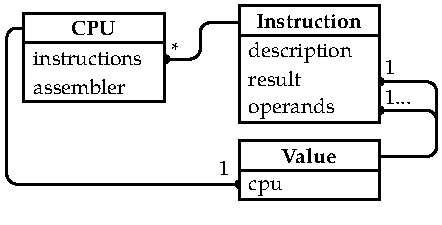
\includegraphics[scale=\imagescale]{vcpu-overview}
	\caption{\VCPU Overview}
	\figlabel{future-vcpu-overview}
\end{figure}
%
\begin{description}
	\item[\CPUs:] Source for values named \ttt{cpu} in the previous examples.
	The \CPU object will contain the list of instructions and for which backend it should generate the native code.
	Additionally we provide specialized \CPU objects for debugging purposes or even immediate evaluation.
	
	\item[Low-level Objects or Values:] A category of values or helper objects.
	For example \ttt{cpu uint: 1} will create low-level word that contains the value \ttt{1}.
	The corresponding high-level equivalent would be a variable.
	In the final native code such a value object might be mapped to a register or stack location.
	Another example is the special low-level object that is the result of a comparison, for instance created by \ttt{a = b}.
	This object holds the result of the comparison and implements the known boolean messages such as \ttt{ifTrue:ifFalse:} or \ttt{and:}.
			
	\item[Instructions:] Encapsulates an instruction type, operands and result value according to the \TAC format.
	Much like in \PH the programmer will almost never directly interact with instructions but with the yielded value. 
	For example \ttt{temp1 + temp1} yields a new \VCPU value and internally records an add instruction in the \CPU object that created the value in \ttt{temp1}.
\end{description}

\noindent In \VCPU the main responsibility for the programming interface lies on the machine objects.
In contrast to that we see that in \AsmJit the full interface is defined on the \ASM itself.
The intermediate values are almost never used, and even registers only play the role of spectators.
Hence, \VCPU takes full advantage of the different types of values to define a simple \DSL.
This way we are able to for instance create branches and loops following \PH semantics rather low-level jumps and labels. 

\paragraph{\CPU Types}
Typically, the \VCPU programmer will only directly interact with the machine objects.
\VCPU instructions are tracked in the related \CPU object, but usually not accessed directly.
However, the \CPU objects play an important role in the development process.
By default each operation on machine objects is dispatched over the corresponding \CPU object as shown in the following code example for the \ttt{+} operation.
%
\begin{stcode}{4}
MachineObject >> + machineObject
	^ cpu add: self with: machineObject
\end{stcode}
%
So, in the example \ttt{c := a + b}, the result object \ttt{c} is created in the \CPU object by invoking the \ttt{add:with:} method.
This allows us to easily customize the behavior of the \CPU objects.
Currently, we have two types of \CPU objects in use:
\begin{description}
	\item[Generating \CPU:] This \CPU delegates the addition to a low-level builder which keeps track of the corresponding \TAC operation.
	After completing a routine, it will compile the \TAC instruction to native code using the specific \ASM backend.
	
	\item[Evaluating \CPU:] This \CPU object does not keep track of the \TAC operations but directly evaluates them.
	Typically we use this \CPU type for debugging purposes.
	The current setup includes a byte array simulating the native memory.
	The evaluating \CPU gives us a \PH-like debugging behavior with very little additional implementation costs.
\end{description}


\paragraph{\VCPU Optimizations}
To get to the final native instructions the \VCPU infrastructure compiles the high-level \TAC instructions to the specific backend.
The current compiler is divided into the following passes:
%
\begin{itemize}[noitemsep]
	\item Platform Specific Transformation
	\item Register Allocation
	\item Superfluous Assignment Remover
	\item Platform Specific Assembler
\end{itemize}
%
\noindent Currently \VCPU does not include more aggressive optimization techniques such as constant folding or subexpression elimination that are associated with a  \TAC \IR.
The, idea is to move the existing \B applications to this new \VCPU format and share the improvements across all tools.
\todo{It is easy to add SSA and thus simplify certain other implementations like register allocation \cite{Wimm10a}}

\paragraph{Custom Machine Objects}
Using first-class machine objects during for the native code format in \VCPU has a secondary application that is not immediately visible.
At code generation time we can use other machine object than the ones described so far.
This finds a direct application in the \NB \FFI when working with structs.
Instead of manually delegating the code generation for accessing fields of a struct to a mirror object we can use it naturally inside \VCPU code.
The following code example outlines this idea.
\begin{stcode}{}
Benzo vcpu x86 generate: [ :cpu |
	| address struct fieldValue |
	address    := cpu address: 16r1234.
	struct     := MyStructure pointer: address.
	fieldValue := struct field1 ]
\end{stcode}
In this example the \ttt{struct field1} message will create several instructions hidden from the user.
Typically, this involves dereferencing the pointer and masking out the corresponding bits of \ttt{field1} from the memory location. 
The only visible artifact from the outside is the returned result.

\todo{missing conclusion}


% -----------------------------------------------------------------------------
\subsection{Barrier-free Low-level Interaction}
% -----------------------------------------------------------------------------
Shifting from \VM development to the final language-runtime we see a similar issue when it comes to tools that span abstraction levels.
It is not directly possible to inspect low-level objects from language-side.
Focusing the on the \B architecture what comes closes to inspecting low-level objects is the \ttt{struct} support for the \NB \FFI library described in \secref{ffi-newtypes}.
We already use this approach for the \NBJ project to inspect \VM internal meta objects for debugging purposes.
It is important to note that giving access to the \VM internal objects is not permitted in most languages.
The previously mentioned \VM generation frameworks usually have first-class objects for all the \VM internal objects or provide mirror-like facilities to access objects from raw memory.
Usually, none of this structural information survives the \VM compilation phase.
Essentially this leaves the final \VM binary with little or no means for introspection. Of course the same restrictions apply then for language-side tools like \B that want to interact with the \VM internals.

\paragraph{Customized \VM \MOP}
We have seen in \secref{validation-nabujito-problems} for \NBJ that the only way to circumvent such issues is by creating modified \VMs which enable specific interaction points.
There are other \PH-based research projects \cite{Arna13a,Lien08b} that took the same path and created a modified \VM.
We, believe that with an extended low-level \MOP the focus for research projects could shift from the \VM to the language-side.
The final extreme is to have a system that works like the described \Klein \VM where there is no longer a clear distinction of what is \VM-level and what is language-side.

\paragraph{Anticipated Debugging}
For \B we have more modest intermediate goals.
The major drawback for a seamless developer experience is the lack of a dedicate low-level debugging infrastructure.
At this point, \B developers have to rely on 3rd-party C-centric tools for debugging.
Hence, a developer has to decide upfront at which abstraction level the debugging should occur.
Either at high-level without the possibility to deal with low-level errors, or at low-level losing all the inspection capabilities.
Besides the shortcomings that either side of the decision will bring, already the fact that the debugging direction has to be anticipated is inappropriate.

We outlined in \secref{benzo-problems-debugging} already several ways to improve the current debugging situation for \B.
The most important focus is on reducing the cases where the programmer has to anticipate the debugging tool.
Since we have to deal with two very distinct abstraction levels we can not only rely on a pure language-side solution to provide different debuggers \cite{Chis13a}.
The major problem is the serious implications of a low-level error.
Unlike user-level errors they are not well-defined or even contained.
It is astonishingly simple to corrupt the \VM memory while writing low-level code and thus breaking any contract with the \VM code.
However, it is more common to access protected memory due to a wrongly dereferenced pointer.
Hence, the \B should focus on this most common bug by following the solution outlined in \figref{future-benzo-debugger}.
%
\begin{figure}[h]
	\centering
	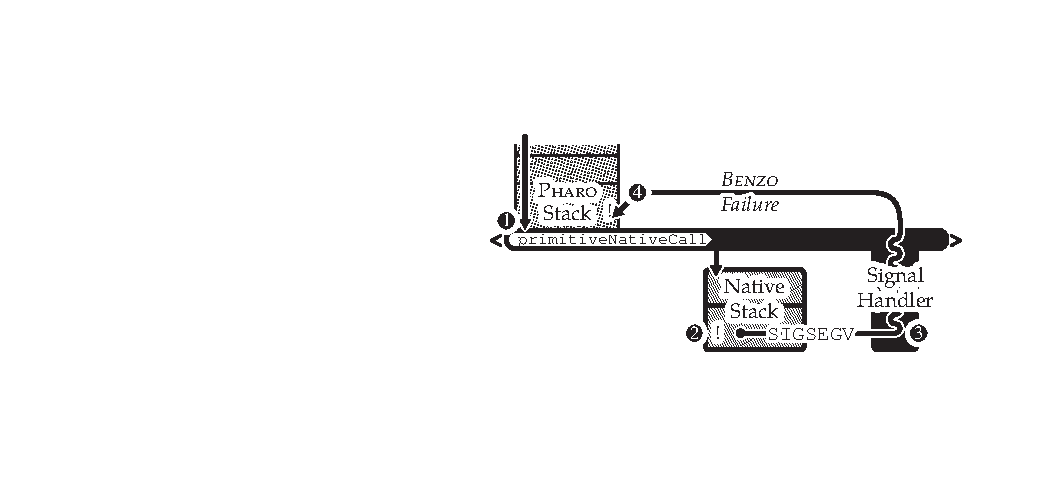
\includegraphics[scale=\imagescale]{benzo-debugger}
	\caption{\B Debugger Outline}
	\figlabel{future-benzo-debugger}
\end{figure}
%
\begin{enumerate}
	\item Standard \PH method activating a \B-enabled method through the \ttt{primitiveNativeCall} primitive.
	\item Native code causing a memory access violation (for example \ttt{SIGSEV}) which can not be handled by \PH directly.
	\item Low-level signal handler is activated by the operating system and tries to walk back the native stack up to the \ttt{primitiveNativeCall} activation.
	\item After successfully finding the \ttt{primitiveNativeCall} the signal handler sends a \B failure back to \PH.
\end{enumerate}

\paragraph{Missing Barrier-free Debugging}
After proposing a solution to improve \B's bug recovery behavior we immediately encounter a second problem.
How do we debug low-level code?
With the aforementioned solution we are able to recover from certain low-level errors and signal them properly at language-side.
In a \ST-like environment the debugger will pop up on the location causing the error and thus allowing a programmer to inspect stack and variables.
To provide the same facility for \B we have to plug into the existing low-level debugging utilities such as \ttt{ptrace} to enable stepping over native instructions.
The following \figref{future-benzo-crossover-debugger} outlines the basics of a debugger that crosses the high-level / low-level barrier.
%
\begin{figure}[h]
	\centering
	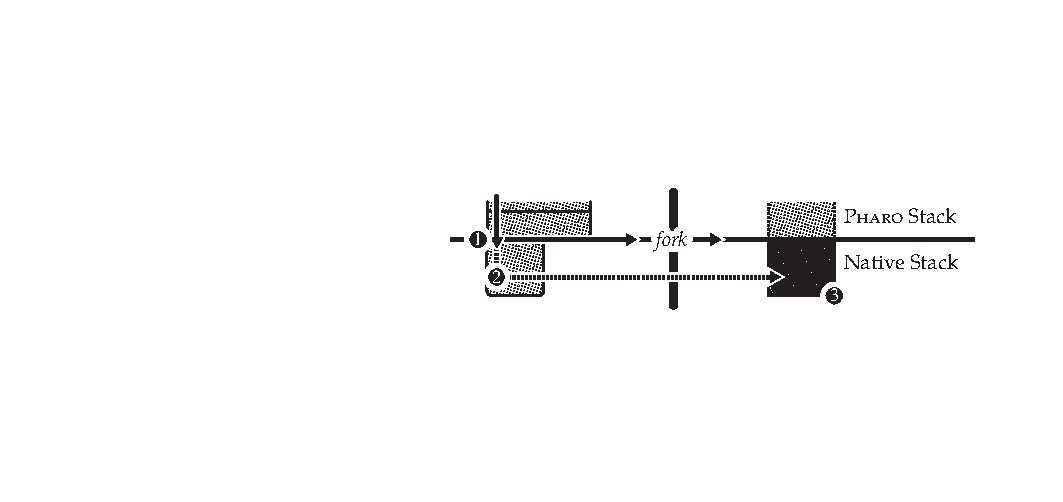
\includegraphics[scale=\imagescale]{benzo-crossover-debugger}
	\caption{\B Crossover Debugger Outline}
	\figlabel{future-benzo-crossover-debugger}
\end{figure}
%
\begin{enumerate}
	\item Point where a \B initiates a native call and the debugger switches from a high-level \PH stack to the low-level native stack.
To properly use low-level debugging tools we fork the complete \VM process.
	\item The low-level debugger in \PH switches the underlying debugging interface.
Instead of directly interacting with first-class \PH context we communicate to the the forked process with tools like \ttt{ptrace}.
	\item The forked process is updated according to the actions initiated from the \PH side.
\end{enumerate}

\noindent The outlined debugger will not work in certain cases where the native code directly interacts with the outer image.
The forked debugger process provides security from the main \PH image by isolating it.
However, for many \B applications such as the \FFI implementation this limitation would not apply.


% =============================================================================
\newpage
\section{\VM-level Improvements}
\seclabel{future-vm}
% =============================================================================
We have presented solutions to improve the code quality and the development experience when working with \B that are focused on the language-side.
We concluded the previous section with the \VCPU intermediate format brings a certain level of platform independence to native code written on the \B.
At even higher-level, we pointed out how the lack of domain specific inspectors prevents a seamless development experience.
The last of the three points present was barrier-free low-level interaction from the language-side point of view.
We mainly focused on the debugger interaction when working with low-level \B code.
One part included the fact that most debugging actions have to be anticipated when working with \B.
This is counter-intuitive to the default \PH development workflow.
However, the solution we presented already required certain \VM-level support to become feasible.

It becomes obvious that a more powerful \B implementation also requires modification at \VM-level.
We explored the limitations of \B with \NBJ the \B-based \JIT compiler presented in \secref{val-nabujito}.
I is not possible to build a \JIT compiler purely on top of \B, instead we had to fall back on a customized \VM with the necessary modifications.
The goal of this section is to outline \VM-level improvements to push the envelope on dynamic changes that extend down to the \VM.
We mainly focus on the reification of \VM-level structure beyond compilation time.
In this sense we follow the findings presented for the \Klein \VM discussed in the related work \secref{future-related-work} of this chapter.
\todo{make obivious that this is the path towards a barrier-free \VM / accessing the 4th quadrant}.
\todo{Tools (NBJ) need access to \VM structures => }\\
\todo{VM structures have to be fully present (conter example is the lack thereof in \P)} \\
\todo{Reifications have to made available to the runtime (introspection / mirror-like)} \\
\todo{Enable dynamic \VM-level intercession by enabling the 4th quadrant} \\
\todo{hand ober FULL control, means that we have to go native at language-side}

\todo{this has to link back to the introduction / problem statement}\\

% -----------------------------------------------------------------------------
\subsection{VM-level Reification}
% -----------------------------------------------------------------------------
\B is a compatible approach to make the low-level power accessible to the language-side.
Yet, it only provides access to native code execution.
Even though this is the basis for generic interaction with the \VM it is too unstructured.

\todo{use the findings from \VM generation frameworks => limits reflection to compilation time => next subsection}\\

\todo{Resulting from the first law of Inspectors, all VM-level objects are reified} \\
\todo{List of typical objects that don't have a reification in COG} \\
\todo{make concepts explicit and first-class} \\
\todo{List advantages: ??? see Klein Paper}\\
\todo{limit the use of raw memory access and string-based programming} \\

% -----------------------------------------------------------------------------
\subsection{Runtime Reification / Dual Objects}
% -----------------------------------------------------------------------------
\todo{Learn from the limitiations of \VM generation frameworks} \\
\todo{Reuse the same objects for the bootstrap and at runtime inspectors/mirrors} \\
\todo{goes further than the sheer compile-time reification of most VM generation frameworks} \\
\todo{accessible from language-side => leads to the following MOP}

% -----------------------------------------------------------------------------
\subsection{Mate Object Model and Runtime MOP}
% -----------------------------------------------------------------------------
\todo{consequence of the runtime reification of the VM introspection => intercession}\\
\todo{Rough Overview of all the Objects currently present in Mate (UMLish)}

% -----------------------------------------------------------------------------
\subsection{Be Native}
% -----------------------------------------------------------------------------
\todo{out of the intercession capabilities follows that we need native support at runtime (see \B)}\\
\todo{that means we need to have decent / better infrasrtucture for native code}\\
\todo{need to be able to achieve what \NBJ didn't manage: compile native methods and hand them over to the \VM}\\
\todo{step towards our implementation in \Mate}


% =============================================================================
\section{\Mate a Reflective \VM Prototype}
\seclabel{mate}
% =============================================================================

\begin{figure*}[h]
	\begin{adjustwidth}{-10.0in}{-10.0in}
		\centering
		
\includegraphics[width=1.02\textwidth]{mate-logo}
	\end{adjustwidth}
\end{figure*}

\todo{introduction: protoype based on the conclusions presented in the previous sections}\\
\todo{for reasearch mainly but possible long term solution to our \VM problems}

% -----------------------------------------------------------------------------
\subsection{Mate Compiler Outline}
\seclabel{future-mate-compiler}
% -----------------------------------------------------------------------------
\todo{Small Intro: Reuse the bootstrap infrastrucutre at runtime (FFI, JIT...)}

\begin{figure}[H]
\centering
	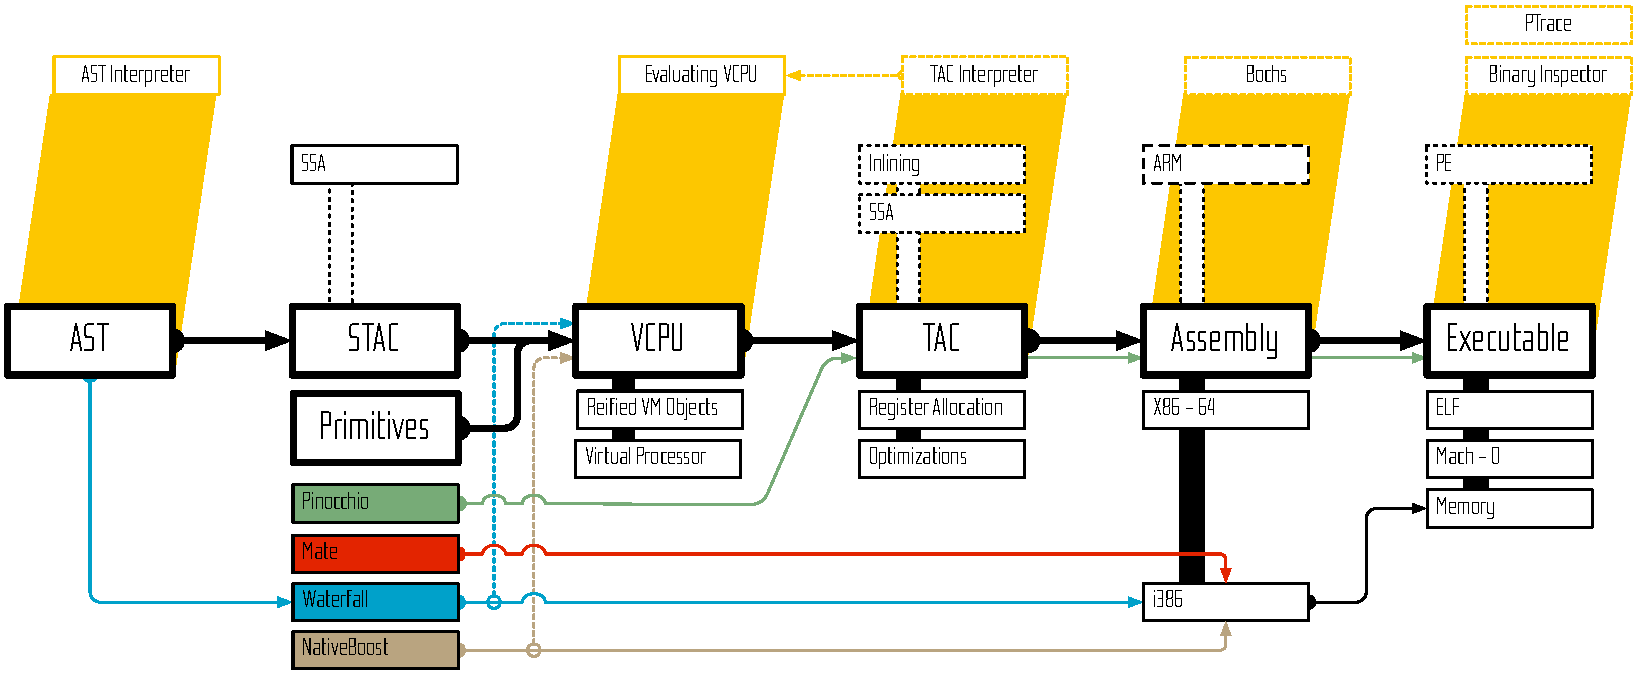
\includegraphics[width=\textwidth]{mate-compilation-toolchain}
\end{figure}

% -----------------------------------------------------------------------------
\subsection{Mate Bootstrap Outline}
\todo{Small Intro: Why Bootstrap and how to use the reified objects}\\
\todo{Compare to Pinocchio (manual approach)}\\
\todo{Work in Progress: Envision the trace-based Bootstrap}


% -----------------------------------------------------------------------------
\subsection{Mate Towards Complete Reflection}
\todo{list possible paths between the 4 quadrants of reflection}\\
\todo{usecase: dynamic gc change}\\
\todo{usecase: dynamic object format influence}\\
\todo{usecase: optimize partial behavior reflection (immutability, proxies)}\\

% =============================================================================
\section{SISTA: Language-side Adaptive Recompilation}
% =============================================================================

\todo{do we put this in a separate section?}\\
\todo{related to \NBJ, but more real-world approach}

% =============================================================================
\section{Reflective Future}
% =============================================================================
% NEW concepts
\todo{Check with GUIDO} \\
\todo{List 3 to 4 different Examples entering the 4th quadrant:}

% -----------------------------------------------------------------------------
\subsection{Accessible VM Components}
% -----------------------------------------------------------------------------
\todo{Access GC Statistics} \\
\todo{Access JIT Statistics for Type Annotations / Tooling}

% -----------------------------------------------------------------------------
\subsection{Interchangeable VM Components}
% -----------------------------------------------------------------------------
\todo{Change GC strategy} \\
\todo{Change JIT Strategy}

% -----------------------------------------------------------------------------
\subsection{Interchangeable Language Semantics}
% -----------------------------------------------------------------------------
\todo{Up to which extent can this be supported?} \\
\todo{Related to VM MOP: How much should be changeable? When?}


% -----------------------------------------------------------------------------
\subsection{Efficient Reflection}
% -----------------------------------------------------------------------------
\todo{Reflectivity at VM-level} \\
\todo{Flatten but don't freeze Reflection/Abstraction}


% =============================================================================
\section{Summary}
% =============================================================================

\todo{a lot of work on the engineering level to get a \VM with reflective properties}\\
\todo{- limited resources focused on maintaining the current infrastructure} \\
\todo{for research we have already sufficient tools at hand to experiment} \\
\todo{- outline some stuff for guido} \\
\todo{possiblity to split up off tools to be used by \PH} \\
\todo{- VCPU IR} \\
\todo{- improved FFI}\\

\todo{link to next section}


% =============================================================================
\ifx\wholebook\relax\else
    \end{document}
\fi
\documentclass[a4paper,12pt,twoside]{../includes/ThesisStyle}
\usepackage[utf8]{inputenc}
\usepackage[T1]{fontenc}

\usepackage[left=1.5in,right=1.3in,top=1.1in,bottom=1.1in,includefoot,includehead,headheight=13.6pt]{geometry}\renewcommand{\baselinestretch}{1.05}


% =============================================================================
%\usepackage[sectionbib]{chapterbib}	% Cross-reference package (Natural BiB)
%\usepackage{bibunits}
%\usepackage{natbib}					% Put References at the end of each chapter
\usepackage{algorithm}
\usepackage{alltt}
\usepackage{amsfonts}
\usepackage{amsmath}
\usepackage{amssymb}
\usepackage{cite}
\usepackage{color}
\usepackage{enumerate}
\usepackage{booktabs} % used for \midrule
\usepackage{fancyhdr}					% Fancy Header and Footer
\usepackage{graphicx}
\usepackage{ifthen}
\usepackage{latexsym}
\usepackage{multirow}
\usepackage{rotating}					% Sideways of figures & tables
\usepackage{stmaryrd}
\usepackage{subfigure}
\usepackage{url}         
\usepackage{xspace}
\usepackage[normalem]{ulem} % for \sout
\usepackage{xcolor}
\usepackage{tablefootnote}
\usepackage{pifont}

% =============================================================================

% Table of contents for each chapter
\usepackage[nottoc, notlof, notlot]{tocbibind}
\usepackage{minitoc}
\setcounter{minitocdepth}{1}
\mtcindent=15pt

\setcounter{secnumdepth}{3}
\setcounter{tocdepth}{2}
  
% =============================================================================
% Fancy Header Style Options

\pagestyle{fancy}                       % Sets fancy header and footer
\fancyfoot{}                            % Delete current footer settings

%\renewcommand{\chaptermark}[1]{         % Lower Case Chapter marker style
%  \markboth{\chaptername\ \thechapter.\ #1}}{}} %

%\renewcommand{\sectionmark}[1]{         % Lower case Section marker style
%  \markright{\thesection.\ #1}}         %

\fancyhead[LE,RO]{\bfseries\thepage}    % Page number (boldface) in left on even
% pages and right on odd pages
\fancyhead[RE]{\bfseries\nouppercase{\leftmark}}      % Chapter in the right on even pages
\fancyhead[LO]{\bfseries\nouppercase{\rightmark}}     % Section in the left on odd pages

\let\headruleORIG\headrule
\renewcommand{\headrule}{\color{black} \headruleORIG}
\renewcommand{\headrulewidth}{1.0pt}
\usepackage{colortbl}
\arrayrulecolor{black}

\fancypagestyle{plain}{
  \fancyhead{}
  \fancyfoot{}
  \renewcommand{\headrulewidth}{0pt}
}


% =============================================================================
% Clear Header Style on the Last Empty Odd pages
\makeatletter

\def\cleardoublepage{\clearpage\if@twoside \ifodd\c@page\else%
  \hbox{}%
  \thispagestyle{empty}%              % Empty header styles
  \newpage%
  \if@twocolumn\hbox{}\newpage\fi\fi\fi}

\makeatother

\newenvironment{maxime}[1]
{
\vspace*{0cm}
\hfill
\begin{minipage}{0.5\textwidth}%
%\rule[0.5ex]{\textwidth}{0.1mm}\\%
\hrulefill $\:$ {\bf #1}\\
%\vspace*{-0.25cm}
\it 
}%
{%

\hrulefill
\vspace*{0.5cm}%
\end{minipage}
}

\let\minitocORIG\minitoc
\renewcommand{\minitoc}{\minitocORIG \vspace{1.5em}}


\renewcommand{\epsilon}{\varepsilon}

% centered page environment
\newenvironment{vcenterpage}
	{\newpage\vspace*{\fill}\thispagestyle{empty}\renewcommand{\headrulewidth}{0pt}}
	{\vspace*{\fill}}
	

%=============================================================================

\usepackage{needspace}
\newcommand{\needlines}[1]{\Needspace{#1\baselineskip}}

\usepackage{xcolor}
\definecolor{source}{gray}{0.95}
% source code formatting
\usepackage{listings}
    % global settings for source code listing package
\lstset{
    basicstyle=\ttfamily\small,
    showspaces=false,
    showstringspaces=false,
    captionpos=b, 
    columns=fullflexible}

\lstdefinelanguage{ST}{
    keywordsprefix=\#,
    morekeywords=[0]{true,false,nil},
    morekeywords=[1]{self,super,thisContext},
    morekeywords=[2]{ifTrue:,ifFalse:,whileTrue:,whileFalse:,and:,or:,xor:,not:,by:,timesRepeat:},
    sensitive=true,
    morecomment=[s]{"}{"},
    morestring=[d]',
    escapechar={!},
    alsoletter={., :, -, =, +, <},
    moredelim=**[is][\itshape]{/+}{+/},
    literate=
        {^}{{$\uparrow$}}1
        {:=}{{$\leftarrow$}}1
        {~}{{$\sim$}}1
        {-}{{\sf -\hspace{-0.13em}-}}1  % the goal is to make - the same width as +
        {+}{\raisebox{0.08ex}{+}}1		% and to raise + off the baseline to match V
        , % Don't forget the comma at the end!
    style=STStyle
}
\lstdefinestyle{STStyle}{
    tabsize=4,
    %frame=leftline,
    % frame=bl,
    %framerule=2pt,
    %rulecolor=\color{gray},
    % backgroundcolor=\color{white},
    %backgroundcolor=\usebeamercolor[bg]{listing},
    basicstyle=\ttfamily\small,
    keywordstyle=\bf\ttfamily,
    % stringstyle=\color{orange},
    stringstyle=\mdseries\slshape,
    commentstyle=\it\rmfamily\color{darkgray}, 
    commentstyle=\mdseries\slshape\color{gray},
    %commentstyle=\mdseries\slshape,
    emphstyle=\bf\ttfamily,
    escapeinside={!}{!},
	%backgroundcolor=\color{source},
    %emphstyle={[2]\color{red}},
    %emphstyle={[3]\color{blue}\bf},
    %emphstyle={[4]\color{blue}},
    keepspaces=true
} 

%\lstnewenvironment{javacode}  [1][]{\lstset{language=java,#1}\needlines{#2}}{} 
%\lstnewenvironment{pythoncode}[2][]{\lstset{language=python,#1}\needlines{#2}}{}
\lstnewenvironment{stcode}    [2][]{\lstset{language=ST,#1}\needlines{#2}}{}
\lstnewenvironment{ccode}     [2][]
    {\lstset{language=C,numbers=left,escapechar=\$,numberstyle=\tiny,#1}\needlines{#2}}{}

% ON: I tried to pass the line number options in as arg #1 but it does not work for me
% I also could net get the line numbers to consistently increase
\lstnewenvironment{numstcode} [2][]
    {\lstset{language=ST,numbers=left,numberstyle=\tiny,numbersep=2pt,#1}\needlines{#2}}{}
\lstnewenvironment{numstcodecont} [2][]
    {\lstset{language=ST,numbers=left,numberstyle=\tiny,numbersep=2pt,firstnumber=last#1}\needlines{#2}}{}

\newcommand{\lst}[1]{{\tt #1}}

% In-line code (literal)

% In-line code (latex enabled)
% Use this only in special situations where \ct does not work
% (within Section headings ...):
\newcommand{\lct}[1]{{\textsf{\textup{#1}}}}
% Code environments
\lstnewenvironment{code}{%
	\lstset{%
		% frame=lines,
		frame=single,
		framerule=0pt,
		mathescape=false
	}
}{}

%\renewcommand{\lstlistingname}{Code Example}

% =============================================================================
\newboolean{showcomments}
\setboolean{showcomments}{true}

\ifthenelse{\boolean{showcomments}} {
	\newcommand{\ugh}[1] {\textcolor{red}{\uwave{#1}}}	% please rephrase
	\newcommand{\ins}[1] {\textcolor{blue}{\uline{#1}}}	% please insert
	\newcommand{\del}[1] {\textcolor{red}{\sout{#1}}}	% please delete
	\newcommand{\chg}[2] {								% please change
		\textcolor{red}{\sout{#1}}{\ra}
		\textcolor{blue}{\uline{#2}}}
	\newcommand{\nbc}[3]{								% comment
		{\colorbox{#3}{\bfseries\sffamily\scriptsize\textcolor{white}{#1}}}
		{\textcolor{#3}{\sf\small$\blacktriangleright$\textit{#2}$\blacktriangleleft$}}}

}{
	\newcommand{\ugh}[1]{#1}							% please rephrase
	\newcommand{\ins}[1]{#1}							% please insert
	\newcommand{\del}[1]{}								% please delete
	\newcommand{\chg}[2]{#2}							% please change
	\newcommand{\nbc}[3]{}								% comment
}

% =============================================================================
\usepackage[pagebackref,hyperindex=true]{hyperref}


% Links in pdf
\usepackage{color}
\definecolor{linkcol}{rgb}{0.0, 0.0, 0.0} 
\definecolor{citecol}{rgb}{0.0, 0.0, 0.0} 

% Change this to change the informations included in the pdf file
% See hyperref documentation for information on those parameters
\hypersetup {
	bookmarksopen=true,
	pdftitle="Design and Use of Anatomical Atlases for Radiotherapy",
	pdfauthor="Olivier COMMOWICK", 
	pdfsubject="Creation of atlases and atlas based segmentation", %subject of the document
	%pdftoolbar=false, % toolbar hidden
	pdfmenubar=true, %menubar shown
	pdfhighlight=/O, %effect of clicking on a link
	colorlinks=true,
	pdfpagemode=UseNone,
	pdfpagelayout=SinglePage,
	pdffitwindow=true,
	linkcolor=linkcol,
	citecolor=citecol,
	urlcolor=linkcol
}

% =============================================================================
\newcommand{\figlabel}[1] {\label{fig:#1}}
\newcommand{\chaplabel}[1]{\label{chap:#1}}
\newcommand{\seclabel}[1] {\label{sec:#1}}
\newcommand{\tablabel}[1] {\label{tab:#1}}
\newcommand{\lstlabel}[1] {\label{lst:#1}}

\newcommand{\figref}[1] {Figure~\ref{fig:#1}}
\newcommand{\chapref}[1]{Chapter~\ref{sec:#1}}
\newcommand{\secref}[1] {Section~\ref{sec:#1}}
\newcommand{\tabref}[1] {Table~\ref{tab:#1}}
\newcommand{\lstref}[1] {Listing~\ref{tab:#1}}

\newcommand{\commented}[1]{}

\newcommand{\bs}    {\symbol{'134}} % backslash
\newcommand{\us}    {\symbol{'137}} % underscore
\newcommand{\ttt}[1]{\texttt{#1}}
\newcommand{\ie}    {\emph{i.e.},\xspace}
\newcommand{\eg}    {\emph{e.g.},\xspace}
\newcommand{\etal}  {\emph{et al.}\xspace}
\newcommand{\ns}    {\!\!\!\!} %big negative space
\newcommand{\cnull} {\textbackslash0\xspace}


\newcommand\fix[1]{\nb{FIX}{#1}}
\newcommand\todo[1]{\nb{TO DO}{#1}}
\newcommand\cb[1]{\nbc{CB}{#1}{purple}}
\newcommand\sd[1]{\nbc{SD}{#1}{orange}}
\newcommand\is[1]{\nbc{IS}{#1}{gray}}
\newcommand\gc[1]{\nbc{GC}{#1}{olive}}
\newcommand\ct[1]{\nbc{CT}{#1}{teal}}
\newcommand\md[1]{\nbc{MD}{#1}{blue}}
\newcommand\dc[1]{\nbc{DC}{#1}{green}}

% =============================================================================
\newcommand{\NBFFI}  {Native\-Boost-FFI\xspace}
\newcommand{\NB}  {Native\-Boost\xspace}
\newcommand{\B}   {Benzo\xspace}
\newcommand{\ST}  {Small\-talk\xspace}
\newcommand{\PH}  {Pharo\xspace}
\graphicspath{{.}{../figures/}}

\begin{document}
% =============================================================================

\chapter{Conclusion}
\chaplabel{conclusion}
\minitoc

% =============================================================================

% =============================================================================
\section{Contributions}
% =============================================================================
\todo{detection of VM level reflectivity => reification?}
\todo{identification of tools that cross vm boundaries}
\todo{identification of partial solution of these tools using benzo}
\todo{identification of the restrictions of a benzo-based tool}
The main contributions of this thesis are:
\begin{enumerate}
	\item Description of the properties of an open and reflective language runtime.
	\item Implementation of 3 main software artifacts to show the feasibility of an open VM.
	\item A roadmap for the future, bottom-up implementation of an open language runtime.
\end{enumerate}

\todo{some prose text}

% =============================================================================
\section{Published Papers}
% =============================================================================
\todo{make subsection + summary (abstract)}
\todo{state to which chapter the papers contributed}
\todo{put all papers with links}
% -----------------------------------------------------------------------------
\subsection{Flexible object layouts: enabling lightweight language extensions by intercepting slot access}
% -----------------------------------------------------------------------------

\todo{write a small intro to describe for which chapter the paper was used}
\begin{description}
	\item[Abstract:] \emph{
Programming idioms, design patterns and application libraries often introduce cumbersome and repetitive boilerplate code to a software system.
Language extensions and external {DSLs} (domain specific languages) are sometimes introduced to reduce the need for boilerplate code, but they also complicate the system by introducing the need for language dialects and inter-language mediation.
To address this, we propose to extend the structural reflective model of the language with object layouts, layout scopes and slots.
Based on the new reflective language model we can 1) provide behavioral hooks to object layouts that are triggered when the fields of an object are accessed and 2) simplify the implementation of state-related language extensions such as stateful traits.
By doing this we show how many idiomatic use cases that normally require boilerplate code can be more effectively supported.
We present an implementation in Smalltalk, and illustrate its usage through a series of extended examples.}

	\item[Authors:] Toon Verwaest, Camillo Bruni, David Gurtner, Adrian Lienhard and Oscar Nierstrasz. 
	\item[Revenue:] In Onward! 2011, Reno/Tahoe, Nevada, USA, 2011.
\end{description}

% -----------------------------------------------------------------------------
\subsection{Language-side Foreign Function Interfaces with NativeBoost}
% -----------------------------------------------------------------------------
\todo{write a small intro to describe for which chapter the paper was used}
\begin{description}
	\item[Abstract:] \emph{
Foreign-Function-Interfaces (FFIs) are a prerequisite for close system integration of a high-level language.
With FFIs the high-level environment interacts with low-level functions allowing for a unique combination of features.
This duality has a strong impact on the implementation of the FFI: it has to be flexible and fast at the same time.
We propose NativeBoost a language-side approach to FFIs that only requires minimal changes to the VM.
NativeBoost directly creates specific native code at language-side and thus combines the flexibility of a language-side library with the performance of a native plugin.}

	\item[Authors:]  Camillo Bruni, Luc Fabresse, Stéphane Ducasse and Igor Stasenko. 
	\item[Revenue:] In International Workshop on Smalltalk Technologies, Annecy, France, 2013.
\end{description}



% =============================================================================
\section{Software Artifacts}
% =============================================================================
\todo{make proper subsections/paragraphs} 
\todo{make sure there is a proper link (arxiv.org... figshare) for each artifact}
\begin{description}
	\item[Collaboration on First-class Layouts and Slots:]
In a collaboration with Toon Verwaest (SCG, Switzerland) we built a first implementation of first-class layouts and slots in a Smalltalk system \cite{Verw11a}.
In Collaboration with Martin Días (RMoD, INRIA) this initial version was ported to Pharo\footnote{\url{}}and is now used in the current release candidate Pharo 3.0\footnote{\url{http://files.pharo.org/image/30}}.

	\item[AsmJIT 64-bit Assembler:]
To reuse the original research compilation pipeline built with Pinocchio \cite{Verw10a, Brun11a} a 64-bit extension was necessary to the initial AsmJit implementation for Pharo\footnote{\url{http://smalltalkhub.com/\#!/~Pharo/AsmJit}}.
The extension is included in the current stable Pharo release 2.0\footnote{\url{http://files.pharo.org/image/20}}.

	\item[Collaboration on the Waterfall Dynamic Primitives:]
We collaborated on the Waterfall Dynamic Primitive compiler together with Guido Chari (UBA, Argentina), which resulted in paper currently under submission\cite{Char13a}.
The implementation is a prototype and is not used in production.

	\item[Collaboration on the Mate VM Prototype:]
In collaboration with Guido Chari (UBA, Argentina), Javier Pímas (UBA, Argentina) and Clement Bera (RMoD, INRIA) several stages of a prototype VM were built.
The implementation mainly follows the concept of an dynamic language runtime which controls every aspect at language-side.
The current language runtime is in a early prototype phase that allows us to explore new VM and language concepts, however it is not production ready.
Guido Chari will further explore new concepts of Mate in his PhD.
Clement Bera, after finishing his engineering contract at RMoD, will continue to work as a PhD on the same system.

	\item[VirtualCPU Compilation Toolchain:]
In collaboration with Clement Bera (RMoD, INRIA) and Igor Stasenko (RMoD, INRIA) we built a prototype compilation toolchain based on the original work of Pinocchio.
The current implementation is a working prototype.
Plans exist to integrate a streamlined version into Pharo to server as a platform independent backend to our Benzo-based FFI implementation used in Pharo.

	\item[Nabujito Language-side JIT Compiler:]
As a third case study for the Benzo framework we implemented a language-side JIT compiler. 
The current implementation is a prototype that is capable of directly transforming simple methods to executable code.
Unlike its VM-level counterpart it is based as a simple visitor over the intermediate bytecode format already present at language-side.

	\item[Inspector Framework for Pharo:] 
An important part of reifying concepts is the possibility to inspect and manipulate these objects.
We wrote a new inspector framework which is used in the latest Pharo release.
It allows to quickly define new views on domain objects, an indispensable requirement for interacting with complex data objects.
Next to the everyday usage in Pharo it is actively used for the Mate VM prototype where we need transparent access to internal structures of the VM.

	\item[Command Line Test Interface for Pharo:]
In order to perform continuous integration in a maintainable fashion we developed a new modular command line interface for Pharo. 
It is used in production on the Pharo build server\footnote{\url{http://ci.inria.fr/pharo/}} alongside with simple installer scripts\footnote{\url{http://get.pharo.org/}}.
\end{description}


% =============================================================================
\section{Future Work}
% =============================================================================
% - go back to all the difficulties identified
% 	 -
% - write possible outline for a future thesis


% =============================================================================
\ifx\wholebook\relax\else
    \end{document}
\fi


% =============================================================================
\appendix
%\include{appendix/def}
% =============================================================================

\bibliographystyle{include/cami}
\bibliography{local}

% =============================================================================
\include{chapter/cv}
\thispagestyle{empty}
% =============================================================================
\end{document}